\documentclass{style}
\usepackage{lipsum}
%定义页面背景色
\definecolor{mycolor01}{RGB}{255, 255, 255}%银河白
\definecolor{mycolor02}{RGB}{250, 249, 222}%杏仁黄
\definecolor{mycolor03}{RGB}{255, 242, 226}%秋叶褐
\definecolor{mycolor04}{RGB}{253, 230, 224}%胭脂红
\definecolor{mycolor05}{RGB}{227, 237, 205}%青草绿
\definecolor{mycolor06}{RGB}{220, 226, 241}%海天蓝
\definecolor{mycolor07}{RGB}{233, 235, 254}%葛巾紫
\definecolor{mycolor08}{RGB}{234, 234, 239}%极光灰
\definecolor{mycolor09}{RGB}{199, 237, 204}%豆沙绿

%设置背景颜色
\pagecolor{mycolor01}	% mycolor01 - mycolor09

\newcommand{\checkpagenumber}{
  \ifodd\thepage
    \newpage\hbox{}
  \else
    % 当前页是偶数页,无需插入空白页
  \fi
}

\begin{document}

%设置说明

% \TiGanSpace 题干说明和题目之间的间距
% \cloze 完型填空
% \fourchoices 选择题
% \lineread 阅读理解横线
% \linefill 新题型横线
% listmatch 新题型列表环境
% \transnum 翻译标号
% listwrite 作文列表环境

%\newlinespread{1.3}{内容} 手动调整行间距

%大写罗马字母 \lmd{2}
%小写罗马字母 \lmx{2}

%封面


\pagestyle{empty}
\rule{0pt}{1pt}
\vfil
\begin{center}
	\heiti \zihao{3}
	   全国硕士研究生入学考试 \\ 
	   英语(一)2001--2023 年真题集 
\end{center}

\vfil


%说明





\chapter*{说 \quad 明}
\thispagestyle{empty}




\rule{2em}{0pt}一年的时光已然匆匆,于此感谢各位小伙伴的帮助和分享。
各年份的真题,可能存在一些拼写错误、标点符号错误等。
这些问题,有待各位共同发现修改。
当各位在用此真题集时,若能顺手,发现错误,指出来,或提交到码云,或者直接拿此源文件修改后分享出来,鄙人不胜感激。愿:
\begin{center}
	\kaishu 
	“古今共栽树,天下齐乘凉”
\end{center}
\begin{center}
	\flushright
	\begin{tabular}{c}
		水   \\
		\today
	\end{tabular}	
\end{center}

\vfil
\noindent
\textcolor{red}{本文档使用 \LaTeX 编写而成,源码地址 \url{https://gitee.com/ylxdxx/EN201-kaoyan}  }
\vfil

\pagestyle{fancy}




%一年一份
%从2013年开始实体书和网络上流传的真题开始不一样
%主要是选项的顺序不一样(包含所有的选择部分)
%选项的顺序应该被人为的修改过,对答案的时候需注意
%后期把答案做进去后,就基本无影响


\bta{2001}

\section{Use of English}

\noindent
\textbf{Directions:}\\
For each numbered blank in the following passage, there are four
	choices marked A, B,
	C. and
	D.  Choose the best
	one and mark your answer on ANSWER SHEET 1 by blackening the
	corresponding letter in the brackets with a pencil. (10 points)


\TiGanSpace

The government is to ban payments to witnesses by newspapers seeking to
buy up people involved in prominent cases \cloze the trial of
Rosemary West.

In a significant \cloze of legal controls over the press, Lord
Irvine, the Lord Chancellor, will introduce a \cloze bill that
will propose making payments to witnesses \cloze and will
strictly control the amount of \cloze that can be given to a case
\cloze a trial begins.

In a letter to Gerald Kaufman, chairman of the House of Commons media
select committee, Lord Irvine said he \cloze with a committee
report this year which said that self regulation did not \cloze
sufficient control.

\cloze of the letter came two days after Lord Irvine caused a
\cloze of media protest when he said the \cloze of
privacy controls contained in European legislation would be left to
judges \cloze to Parliament.

The Lord Chancellor said introduction of the Human Rights Bill, which
\cloze the European Convention on Human Rights legally
\cloze in Britain, laid down that everybody was \cloze
to privacy and that public figures could go to court to protect
themselves and their families.

``Press freedoms will be in safe hands \cloze our British
judges,'' he said.

Witness payments became an \cloze after West was sentenced to 10
life sentences in 1995. Up to 19 witnesses were \cloze to have
received payments for telling their stories to newspapers. Concerns were
raised \cloze witnesses might be encouraged exaggerate their
stories in court to \cloze guilty verdicts.


\newpage
\begin{enumerate}
	%\renewcommand{\labelenumi}{\arabic{enumi}.}
	% A(\Alph) a(\alph) I(\Roman) i(\roman) 1(\arabic)
	%设定全局标号series=example	%引用全局变量resume=example
	%[topsep=-0.3em,parsep=-0.3em,itemsep=-0.3em,partopsep=-0.3em]
	%可使用leftmargin调整列表环境左边的空白长度 [leftmargin=0em]
	\item

\fourchoices
{as to}
{for instance}
{in particular}
{such as}




\item


\fourchoices
{tightening}
{intensifying}
{focusing}
{fastening}




\item


\fourchoices
{sketch}
{rough}
{preliminary}
{draft}




\item


\fourchoices
{illogical}
{illegal}
{improbable}
{improper}




\item


\fourchoices
{publicity}
{penalty}
{popularity}
{peculiarity}




\item


\fourchoices
{since}
{if}
{before}
{as}




\item


\fourchoices
{sided}
{shared}
{complied}
{agreed}




\item


\fourchoices
{present}
{offer}
{manifest}
{indicate}




\item


\fourchoices
{Release}
{Publication}
{Printing}
{Exposure}




\item


\fourchoices
{storm}
{rage}
{flare}
{flash}




\item

\fourchoices
{translation}
{interpretation}
{exhibition}
{demonstration}



\item


\fourchoices
{better than}
{other than}
{rather than}
{sooner than}




\item


\fourchoices
{changes}
{makes}
{sets}
{turns}




\item


\fourchoices
{binding}
{convincing}
{restraining}
{sustaining}




\item


\fourchoices
{authorized}
{credited}
{entitled}
{qualified}




\item


\fourchoices
{with}
{to}
{from}
{by}




\item


\fourchoices
{impact}
{incident}
{inference}
{issue}




\item


\fourchoices
{stated}
{remarked}
{said}
{told}




\item

\fourchoices
{what}
{when}
{which}
{that}




\item


\fourchoices
{assure}
{confide}
{ensure}
{guarantee}

\end{enumerate}

\vfil

\section{ Reading Comprehension}

\noindent
\textbf{Directions:}\\
Each of the passages below is followed by some questions. For
each questions there are four answers marked A, B,
C.
and
D.  Read the passages carefully and choose the best answer to
each of the questions. Then mark your answer on ANSWER SHEET 1 by
blackening the corresponding letter in the brackets with a pencil. (40
points)


\newpage

\subsection{Passage 1}

Specialisation can be seen as a response to the problem of an increasing
accumulation of scientific knowledge. By splitting up the subject matter
into smaller units, one man could continue to handle the information and
use it as the basis for further research. But specialisation was only
one of a series of related developments in science affecting the process
of communication. Another was the growing professionalisation of
scientific activity.

No clear-cut distinction can be drawn between professionals and amateurs
in science: exceptions can be found to any rule. Nevertheless, the word ``amateur'' does carry a connotation that the person concerned is not
fully integrated into the scientific community and, in particular, may
not fully share its values. The growth of specialisation in the
nineteenth century, with its consequent requirement of a longer, more
complex training, implied greater problems for amateur participation in
science. The trend was naturally most obvious in those areas of science
based especially on a mathematical or laboratory training, and can be
illustrated in terms of the development of geology in the United
Kingdom.

A comparison of British geological publications over the last century
and a half reveals not simply an increasing emphasis on the primacy of
research, but also a changing definition of what constitutes an
acceptable research paper. Thus, in the nineteenth century, local
geological studies represented worthwhile research in their own right;
but, in the twentieth century, local studies have increasingly become
acceptable to professionals only if they incorporate, and reflect on,
the wider geological picture. Amateurs, on the other hand, have
continued to pursue local studies in the old way. The overall result has
been to make entrance to professional geological journals harder for
amateurs, a result that has been reinforced by the widespread
introduction of refereeing, first by national journals in the nineteenth
century and then by several local geological journals in the twentieth
century. As a logical consequence of this development, separate journals
have now appeared aimed mainly towards either professional or amateur
readership. A rather similar process of differentiation has led to
professional geologists coming together nationally within one or two
specific societies, whereas the amateurs have tended either to remain in
local societies or to come together nationally in a different way.

Although the process of professionalisation and specialisation was
already well under way in British geology during the nineteenth century,
its full consequences were thus delayed until the twentieth century. In
science generally, however, the nineteenth century must be reckoned as
the crucial period for this change in the structure of science.


\begin{enumerate}[resume]
	%\renewcommand{\labelenumi}{\arabic{enumi}.}
	% A(\Alph) a(\alph) I(\Roman) i(\roman) 1(\arabic)
	%设定全局标号series=example	%引用全局变量resume=example
	%[topsep=-0.3em,parsep=-0.3em,itemsep=-0.3em,partopsep=-0.3em]
	%可使用leftmargin调整列表环境左边的空白长度 [leftmargin=0em]
	\item
The growth of specialisation in the 19th century might be more
clearly seen in sciences such as \lineread.

\fourchoices
{sociology and chemistry}
{physics and psychology}
{sociology and psychology}
{physics and chemistry}



\item
We can infer from the passage that \lineread.


\fourchoices
{there is little distinction between specialisation and professionalisation}
{amateurs can compete with professionals in some areas of science}
{professionals tend to welcome amateurs into the scientific community}
{amateurs have national academic societies but no local ones}



\item
The author writes of the development of geology to demonstrate \lineread.


\fourchoices
{the process of specialisation and professionalisation}
{the hardship of amateurs in scientific study}
{the change of policies in scientific publications}
{the discrimination of professionals against amateurs}



\item
The direct reason for specialisation is \lineread.


\fourchoices
{the development in communication}
{the growth of professionalisation}
{the expansion of scientific knowledge}
{the splitting up of academic societies}

\end{enumerate}

\newpage

\subsection{Passage 2}

A great deal of attention is being paid today to the so-called digital
divide---the division of the world into the info (information) rich and
the info poor. And that divide does exist today. My wife and I lectured
about this looming danger twenty years ago. What was less visible then,
however, were the new, positive forces that work against the digital
divide. There are reasons to be optimistic.

There are technological reasons to hope the digital divide will narrow.
As the Internet becomes more and more commercialized, it is in the
interest of business to universalize access---after all, the more people
online, the more potential customers there are. More and more
governments, afraid their countries will be left behind, want to spread
Internet access. Within the next decade or two, one to two billion
people on the planet will be netted together. As a result, I now believe
the digital divide will narrow rather than widen in the years ahead. And
that is very good news because the Internet may well be the most
powerful tool for combating world poverty that we've ever had.

Of course, the use of the Internet isn't the only way to defeat poverty.
And the Internet is not the only tool we have. But it has enormous
potential.

To take advantage of this tool, some impoverished countries will have to
get over their outdated anti-colonial prejudices with respect to foreign
investment. Countries that still think foreign investment is an invasion
of their sovereignty might well study the history of infrastructure (the
basic structural foundations of a society) in the United States. When
the United States built its industrial infrastructure, it didn't have
the capital to do so. And that is why America's Second Wave
infrastructure---including roads, harbors, highways, ports and so on---were
built with foreign investment. The English, the Germans, the Dutch and
the French were investing in Britain's former colony. They financed
them. Immigrant Americans built them. Guess who owns them now? The
Americans. I believe the same thing would be true in places like Brazil
or anywhere else for that matter. The more foreign capital you have
helping you build your Third Wave infrastructure, which today is an
electronic infrastructure, the better off you're going to be. That
doesn't mean lying down and becoming fooled, or letting foreign
corporations run uncontrolled. But it does mean recognizing how
important they can be in building the energy and telecom infrastructures
needed to take full advantage of the Internet.


\begin{enumerate}[resume]
	%\renewcommand{\labelenumi}{\arabic{enumi}.}
	% A(\Alph) a(\alph) I(\Roman) i(\roman) 1(\arabic)
	%设定全局标号series=example	%引用全局变量resume=example
	%[topsep=-0.3em,parsep=-0.3em,itemsep=-0.3em,partopsep=-0.3em]
	%可使用leftmargin调整列表环境左边的空白长度 [leftmargin=0em]
	\item
Digital divide is something \lineread.


\fourchoices
{getting worse because of the Internet}
{the rich countries are responsible for}
{the world must guard against}
{considered positive today}


\item
 Governments attach importance to the Internet because it \lineread.


\fourchoices
{offers economic potentials}
{can bring foreign funds}
{can soon wipe out world poverty}
{connects people all over the world}


\item
The writer mentioned the case of the United States to justify the
policy of \lineread.


\fourchoices
{providing financial support overseas}
{preventing foreign capital's control}
{building industrial infrastructure}
{accepting foreign investment}



\item
It seems that now a country's economy depands much on \lineread.


\fourchoices
{how well-developed it is electronically}
{whether it is prejudiced against immigrants}
{whether it adopts America's industrial pattern}
{how much control it has over foreign corporations}
	
\end{enumerate}



\newpage
\subsection{Passage 3}

Why do so many Americans distrust what they read in their newspapers?
The American Society of Newspaper Editors is trying to answer this
painful question. The organization is deep into a long self-analysis
known as the journalism credibility project.

Sad to say, this project has turned out to be mostly low-level findings
about factual errors and spelling and grammar mistakes, combined with
lots of head-scratching puzzlement about what in the world those readers
really want.

But the sources of distrust go way deeper. Most journalists learn to see
the world through a set of standard templates (patterns) into which they
plug each day's events. In other words, there is a conventional story
line in the newsroom culture that provides a backbone and a ready-made
narrative structure for otherwise confusing news.

There exists a social and cultural disconnect between journalists and
their readers which helps explain why the ``standard templates''of the
newsroom seem alien to many readers. In a recent survey, questionnaires
were sent to reporters in five middle size cities around the country,
plus one large metropolitan area. Then residents in these communities
were phoned at random and asked the same questions.

Replies show that compared with other Americans, journalists are more
likely to live in upscale neighborhoods, have maids, own Mercedeses, and
trade stocks, and they're less likely to go to church, do volunteer
work, or put down roots in community.

Reporters tend to be part of a broadly defined social and cultural
elite, so their work tends to reflect the conventional values of this
elite. The astonishing distrust of the news media isn't rooted in
inaccuracy or poor reportorial skills but in the daily clash of world
views between reporters and their readers.

This is an explosive situation for any industry, particularly a
declining one. Here is a troubled business that keeps hiring employees
whose attitudes vastly annoy the customers. Then it sponsors lots of
symposiums and a credibility project dedicated to wondering why
customers are annoyed and fleeing in large numbers. But it never seems
to get around to noticing the cultural and class biases that so many
former buyers are complaining about. If it did, it would open up its
diversity program, now focused narrowly on race and gender, and look for
reporters who differ broadly by outlook, values, education, and class.


\begin{enumerate}[resume]
	%\renewcommand{\labelenumi}{\arabic{enumi}.}
	% A(\Alph) a(\alph) I(\Roman) i(\roman) 1(\arabic)
	%设定全局标号series=example	%引用全局变量resume=example
	%[topsep=-0.3em,parsep=-0.3em,itemsep=-0.3em,partopsep=-0.3em]
	%可使用leftmargin调整列表环境左边的空白长度 [leftmargin=0em]
	\item
What is the passage mainly about?


\fourchoices
{Needs of the readers all over the world.}
{Causes of the public disappointment about newspapers.}
{Origins of the declining newspaper industry.}
{Aims of a journalism credibility project.}



\item
The results of the journalism credibility project turned out to be \lineread.


\fourchoices
{quite trustworthy}
{somewhat contradictory}
{very illuminating}
{rather superficial}


\item
The basic problem of journalists as pointed out by the writer lies
in their \lineread.


\fourchoices
{working attitude}
{conventional lifestyle}
{world outlook}
{educational background}


\item
Despite its efforts, the newspaper industry still cannot satisfy the
readers owing to its \lineread.


\fourchoices
{failure to realize its real problem}
{tendency to hire annoying reporters}
{likeliness to do inaccurate reporting}
{prejudice in matters of race and gender}


\end{enumerate}


\newpage
\subsection{Passage 4}

The world is going through the biggest wave of mergers and acquisitions
ever witnessed. The process sweeps from hyperactive America to Europe
and reaches the emerging countries with unsurpassed might. Many in these
countries are looking at this process and worrying: " Won't the wave of
business concentration turn into an uncontrollable anti-competitive
force?"

There's no question that the big are getting bigger and more powerful.
Multinational corporations accounted for less than 20\% of international
trade in 1982. Today the figure is more than 25\% and growing rapidly.
International affiliates account for a fast-growing segment of
production in economies that open up and welcome foreign investment. In
Argentina, for instance, after the reforms of the early 1990 s,
multinationals went from 43\% to almost 70\% of the industrial
production of the 200 largest firms. This phenomenon has created serious
concerns over the role of smaller economic firms, of national
businessmen and over the ultimate stability of the world economy.

I believe that the most important forces behind the massive M\&A wave
are the same that underlie the globalization process: falling
transportation and communication costs, lower trade and investment
barriers and enlarged markets that require enlarged operations capable
of meeting customers' demands. All these are beneficial, not
detrimental, to consumers. As productivity grows, the world's wealth
increases.

Examples of benefits or costs of the current concentration wave are
scanty. Yet it is hard to imagine that the merger of a few oil firms
today could re-create the same threats to competition that were feared
nearly a century ago in the U.S., when the Standard Oil trust was broken
up. The mergers of telecom companies, such as WorldCom, hardly seem to
bring higher prices for consumers or a reduction in the pace of
technical progress. On the contrary, the price of communications is
coming down fast. In cars, too, concentration is increasing---witness
Daimler and Chrysler, Renault and Nissan-but it does not appear that
consumers are being hurt.

Yet the fact remains that the merger movement must be watched. A few
weeks ago, Alan Greenspan warned against the megamergers in the banking
industry. Who is going to supervise, regulate and operate as lender of
last resort with the gigantic banks that are being created? Won't
multinationals shift production from one place to another when a nation
gets too strict about infringements to fair competition? And should one
country take upon itself the role of ``defending competition'' on issues
that affect many other nations, as in the U.S. vs. Microsoft case?


\begin{enumerate}[resume]
	%\renewcommand{\labelenumi}{\arabic{enumi}.}
	% A(\Alph) a(\alph) I(\Roman) i(\roman) 1(\arabic)
	%设定全局标号series=example	%引用全局变量resume=example
	%[topsep=-0.3em,parsep=-0.3em,itemsep=-0.3em,partopsep=-0.3em]
	%可使用leftmargin调整列表环境左边的空白长度 [leftmargin=0em]
	\item
What is the typical trend of businesses today?


\fourchoices
{To take in more foreign funds.}
{To invest more abroad.}
{To combine and become bigger.}
{To trade with more countries.}


\item
According to the author, one of the driving forces behind M\&A wave
is \lineread


\fourchoices
{the greater customer demands.}
{a surplus supply for the market.}
{a growing productivity.}
{the increase of the world's wealth.}


\item
From paragraph 4 we can infer that \lineread.


\fourchoices
{the increasing concentration is certain to hurt consumers}
{WorldCom serves as a good example of both benefits and costs}
{the costs of the globalization process are enormous}
{the Standard Oil trust might have threatened competition}



\item
Toward the new business wave, the writer's attitude can he said to
be \lineread.


\fourchoices
{optimistic}
{objective}
{pessimistic}
{biased}

	
\end{enumerate}



\newpage
\subsection{Passage 5}

When I decided to quit my full time employment it never occurred to me
that I might become a part of a new international trend. A lateral move
that hurt my pride and blocked my professional progress prompted me to
abandon my relatively high profile career although, in the manner of a
disgraced government minister, I covered my exit by claiming ``I wanted
to spend more time with my family''.

Curiously, some two-and-a-half years and two novels later, my experiment
in what the Americans term ``downshifting''has turned my tired excuse
into an absolute reality. I have been transformed from a passionate
advocate of the philosophy of ``having it all'', preached by Linda
Kelsey for the past seven years in the pages of She magazine, into a
woman who is happy to settle for a bit of everything.

I have discovered, as perhaps Kelsey will after her much-publicized
resignation from the editorship of She after a build-up of stress, that
abandoning the doctrine of ``juggling your life'', and making the
alternative move into ``downshifting'' brings with it far greater
rewards than financial success and social status. Nothing could persuade
me to return to the kind of life Kelsey used to advocate and I once
enjoyed: 12-hour working days, pressured deadlines, the fearful strain
of office politics and the limitations of being a parent on ``quality
time''.

In America, the move away from juggling to a simpler, less materialistic
lifestyle is a well-established trend. Downshifting-also known in
America as ``voluntary simplicity''---has, ironically, even bred a new
area of what might be termed anticonsumerism. There are a number of
best-selling downshifting self-help books for people who want to simplify
their lives; there are newsletter's, such as The Tightwad Gazette, that
give hundreds of thousands of Americans useful tips on anything from
recycling their cling-film to making their own soap; there are even
support groups for those who want to achieve the mid- '90s equivalent of
dropping out.

While in America the trend started as a reaction to the economic
decline---after the mass redundancies caused by downsizing in the
late '80s---and is still linked to the politics of thrift, in Britain,
at least among the middle-class downshifters of my acquaintance, we have
different reasons for seeking to simplify our lives.

For the women of my generation who were urged to keep juggling through
the'80 s, downshifting in the mid-'90s is not so much a search for the
mythical good life---growing your own organic vegetables, and risking
turning into one---as a personal recognition of your limitations.

\begin{enumerate}[resume]
	%\renewcommand{\labelenumi}{\arabic{enumi}.}
	% A(\Alph) a(\alph) I(\Roman) i(\roman) 1(\arabic)
	%设定全局标号series=example	%引用全局变量resume=example
	%[topsep=-0.3em,parsep=-0.3em,itemsep=-0.3em,partopsep=-0.3em]
	%可使用leftmargin调整列表环境左边的空白长度 [leftmargin=0em]
	\item
Which of the following is true according to paragraph 1?


\fourchoices
{Full-time employment is a new international trend.}
{The writer was compelled by circumstances to leave her job.}
{``A lateral move'' means stepping out of full-time employment.}
{The writer was only too eager to spend more time with her family.}



\item
The writer's experiment shows that downshifting \lineread


\fourchoices
{enables her to realize her dream}
{helps her mold a new philosophy of life}
{prompts her to abandon her high social status}
{leads her to accept the doctrine of \emph{She} magazine}


\item
``Juggling one's life'' probably means living a life characterized
by \lineread.


\fourchoices
{non-materialistic lifestyle}
{a bit of everything}
{extreme stress}
{anti-consumerism}


\item
According to the passage, downshifting emerged in the U.S. as a
result of \lineread


\fourchoices
{the quick pace of modern life}
{man's adventurous spirit}
{man's search for mythical experiences}
{the economic situation}

	
\end{enumerate}


\newpage
\section{ English-Chinese Translation}

\noindent
\textbf{Directions:}\\
Read the following text carefully and then translate the
underlined segments into Chinese. Your translation should be written
clearly on ANSWER SHEET 2. (15 points)

\TiGanSpace

In less than 30 years' time the \emph{Star Trek} holodeck will be a reality.
Direct links between the brain's nervous system and a computer will also
create full sensory virtual environments, allowing virtual vacations
like those in the film \emph{Total Recall}.



\transnum \uline{There will be television chat shows hosted by robots, and
cars with pollution monitors that will disable them when they offend}.
\transnum \uline{Children will play with dolls equipped with personality
chips, computers with in-built personalities will be regarded as
workmates rather than tools, relaxation will be in front of smell-television, and digital age will have arrived.}

According to BT's futurologist, Ian Pearson, these are among the
developments scheduled for the first few decades of the new
millennium (a period of 1,000 years), when supercomputers will
dramatically accelerate progress in all areas of life.

\transnum \uline{Pearson has pieced together the work of hundreds of
researchers around the world to produce a unique millennium technology
calendar that gives the latest dates when we can expect hundreds of key
breakthroughs and discoveries to take place.} Some of the biggest
developments will be in medicine, including an extended life expectancy
and dozens of artificial organs coming into use between now and 2040.

Pearson also predicts a breakthrough in computer-human links. ``By
linking directly to our nervous system, computers could pick up what we
feel and, hopefully, simulate feeling too so that we can start to
develop full sensory environments, rather like the holidays in \emph{Total Recall} or the \emph{Star Trek} holodeck,'' he says. \transnum \uline{But that,
Pearson points out, is only the start of man-machine integration: ``It
will be the beginning of the long process of integration that will
ultimately lead to a fully electronic human before the end of the next
century}.''

Through his research, Pearson is able to put dates to most of the
breakthroughs that can be predicted. However, there are still no
forecasts for when faster-than-light travel will be available, or when
human cloning will be perfected, or when time travel will be possible.
But he does expect social problems as a result of technological
advances. A boom in neighborhood surveillance cameras will, for example,
cause problems in 2010, while the arrival of synthetic lifelike robots
will mean people may not be able to distinguish between their human
friends and the droids.
\transnum \uline{And home appliances will also become so smart that
controlling and operating them will result in the breakout of a new
psychological disorder---kitchen rage.}




\section{Writing}


\noindent
\textbf{46. Directions:}

Among all the worthy feelings of mankind, love is probably the noblest,
but everyone has his/her own understanding of it.

There has been a discussion recently on the issue in a newspaper. Write
an essay to the newspaper to
\begin{listwrite}
	\item 
show your understanding of the symbolic meaning of the picture below,

\item 
give a specific example, and

\item 
give your suggestion as to the best way to show love.

\end{listwrite}

You should write about 200 words neatly on ANSWER SHEET 2. (20 points)

\begin{figure}[h!]
	\centering
	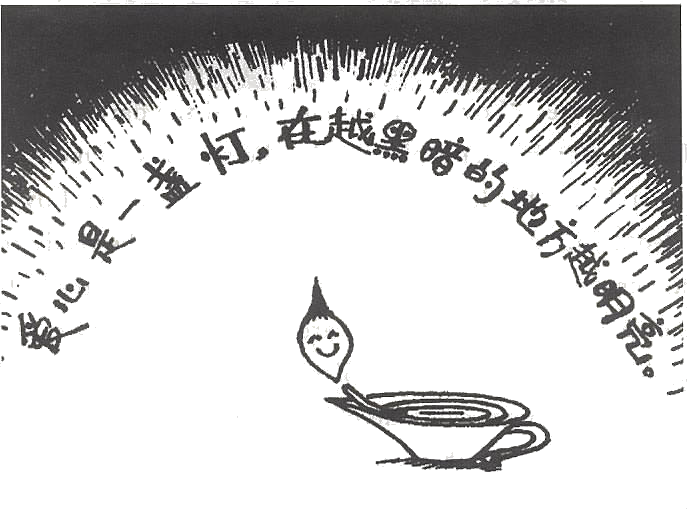
\includegraphics[width=0.5\linewidth]{picture/2001.png}
\end{figure}





\bta{2002}

\section{Use of English}

\noindent
\textbf{Directions:}\\
Read the following text. Choose the best word (s) for each
	numbered blank and mark A, B, C OR D on ANSWER SHEET 1. (10 points)

\TiGanSpace

Comparisons were drawn between the development of television in the 20th
century and the diffusion of printing in the 15th and 16th centuries.
Yet much had happened \cloze. As was discussed before, it was
not \cloze the 19th century that the newspaper became the
dominant pre-electronic \cloze , following in the wake of
the pamphlet and the book and in the \cloze of the periodical. It
was during the same time that the communications revolution
\cloze up, beginning with transport, the railway, and leading
\cloze through the telegraph, the telephone, radio, and motion
pictures \cloze the 20th century world of the
motor car and the air plane. Not everyone sees that Process in
\cloze. It is important to do so.

It is generally recognized, \cloze , that the introduction of the
computer in the early 20th century, \cloze by the invention of
the integrated circuit during the 1960 s, radically changed the process,
\cloze its impact on the media was not immediately
\cloze. As time went by, computers became smaller and more
powerful, and they became ``personal'' too, as well as \cloze ,
with display becoming sharper and storage \cloze increasing.
They were thought of, like people, \cloze generations, with the
distance between generations much \cloze.

It was within the computer age that the term ``information society''
began to be widely used to describe the \cloze within which we
now live. The communications revolution has \cloze both work and
leisure and how we think and feel both about place and time, but there
have been \cloze view about its economic, political, social and
cultural implications. ``Benefits'' have been weighed \cloze
``harmful'' outcomes. And generalizations have proved difficult.


\newpage
\begin{enumerate}
	%\renewcommand{\labelenumi}{\arabic{enumi}.}
	% A(\Alph) a(\alph) I(\Roman) i(\roman) 1(\arabic)
	%设定全局标号series=example	%引用全局变量resume=example
	%[topsep=-0.3em,parsep=-0.3em,itemsep=-0.3em,partopsep=-0.3em]
	%可使用leftmargin调整列表环境左边的空白长度 [leftmargin=0em]
	\item


\fourchoices
{between}
{before}
{since}
{later}




\item


\fourchoices
{after}
{by}
{during}
{until}




\item


\fourchoices
{means}
{method}
{medium}
{measure}




\item


\fourchoices
{process}
{company}
{light}
{form}




\item


\fourchoices
{gathered}
{speeded}
{worked}
{picked}




\item


\fourchoices
{on}
{out}
{over}
{off}




\item


\fourchoices
{of}
{for}
{beyond}
{into}




\item


\fourchoices
{concept}
{dimension}
{effect}
{perspective}




\item


\fourchoices
{indeed}
{hence}
{however}
{therefore}




\item


\fourchoices
{brought}
{followed}
{stimulated}
{characterized}




\item


\fourchoices
{unless}
{since}
{lest}
{although}




\item


\fourchoices
{apparent}
{desirable}
{negative}
{plausible}




\item


\fourchoices
{institutional}
{universal}
{fundamental}
{instrumental}




\item


\fourchoices
{ability}
{capability}
{capacity}
{faculty}




\item


\fourchoices
{by means of}
{in terms of}
{with regard to}
{in line with}





\item


\fourchoices
{deeper}
{fewer}
{nearer}
{smaller}




\item


\fourchoices
{context}
{range}
{scope}
{territory}




\item


\fourchoices
{regarded}
{impressed}
{influenced}
{effected}




\item


\fourchoices
{competitive}
{controversial}
{distracting}
{irrational}




\item


\fourchoices
{above}
{upon}
{against}
{with}

\end{enumerate}

\vfil

\section{Reading Comprehension}






\noindent
\textbf{Part A}\\
\textbf{Directions:}\\
Read the following four texts. Answer the questions below each
	text by choosing A, B, C or
	D. Mark your answers
	on ANSWER SHEET 1. (40 points)

\newpage
\subsection{Text 1}


If you intend using humor in your talk to make people smile, you must
know how to identify shared experiences and problems. Your humor must be
relevant to the audience and should help to show them that you are one
of them or that you understand their situation and are in sympathy with
their point of view. Depending on whom you are addressing, the problems
will be different. If you are talking to a group of managers, you may
refer to the disorganized methods of their secretaries; alternatively if
you are addressing secretaries, you may want to comment on their
disorganized bosses.

Here is an example, which I heard at a nurses' convention, of a story
which works well because the audience all shared the same view of
doctors. A man arrives in heaven and is being shown around by St. Peter.
He sees wonderful accommodations, beautiful gardens, sunny weather, and
so on. Everyone is very peaceful, polite and friendly until, waiting in
a line for lunch, the new arrival is suddenly pushed aside by a man in a
white coat, who rushes to the head of the line, grabs his food and
stomps over to a table by himself. ``Who is that?'' the new arrival
asked St. Peter. ``Oh, that's God,'' came the reply, ``but sometimes he
thinks he's a doctor.''

If you are part of the group which you are addressing, you will be in a
position to know the experiences and problems which are common to all of
you and it'll be appropriate for you to make a passing remark about the
inedible canteen food or the chairman's notorious bad taste in ties.
With other audiences you mustn't attempt to cut in with humor as they
will resent an outsider making disparaging remarks about their canteen
or their chairman. You will be on safer ground if you stick to
scapegoats like the Post Office or the telephone system.

If you feel awkward being humorous, you must practice so that it becomes
more natural. Include a few casual and apparently off-the-cuff remarks
which you can deliver in a relaxed and unforced manner. Often it's the
delivery which causes the audience to smile, so speak slowly and
remember that a raised eyebrow or an unbelieving look may help to show
that you are making a light-hearted remark.

Look for the humor. It often comes from the unexpected. A twist on a
familiar quote ``If at first you don't succeed, give up'' or a play on
words or on a situation. Search for exaggeration and understatement.
Look at your talk and pick out a few words or sentences which you can
turn about and inject with humor.

\begin{enumerate}[resume]
	%\renewcommand{\labelenumi}{\arabic{enumi}.}
	% A(\Alph) a(\alph) I(\Roman) i(\roman) 1(\arabic)
	%设定全局标号series=example	%引用全局变量resume=example
	%[topsep=-0.3em,parsep=-0.3em,itemsep=-0.3em,partopsep=-0.3em]
	%可使用leftmargin调整列表环境左边的空白长度 [leftmargin=0em]
	\item
To make your humor work, you should \lineread.


\fourchoices
{take advantage of different kinds of audience}
{make fun of the disorganized people}
{address different problems to different people}
{show sympathy for your listeners}


\item
The joke about doctors implies that, in the eyes of nurses, they are \lineread.


\fourchoices
{impolite to new arrivals}
{very conscious of their godlike role}
{entitled to some privileges}
{very busy even during lunch hours}


\item
 It can be inferred from the text that public services \lineread.


\fourchoices
{have benefited many people}
{are the focus of public attention}
{are an inappropriate subject for humor}
{have often been the laughing stock}


\item
To achieve the desired result, humorous stories should be delivered \lineread.


\fourchoices
{in well-worded language}
{as awkwardly as possible}
{in exaggerated statements}
{as casually as possible}


\item
The best title for the text may be \lineread.


\fourchoices
{Use Humor Effectively}
{Various Kinds of Humor}
{Add Humor to Speech}
{Different Humor Strategies}

\end{enumerate}


\newpage
\subsection{Text 2}


Since the dawn of human ingenuity, people have devised ever more cunning
tools to cope with work that is dangerous, boring, burdensome, or just
plain nasty. That compulsion has resulted in robotics---the science of
conferring various human capabilities on machines. And if scientists
have yet to create the mechanical version of science fiction, they have
begun to come close.

As a result, the modern world is increasingly populated by intelligent
gizmos whose presence we barely notice but whose universal existence has
removed much human labor. Our factories hum to the rhythm of robot
assembly arms. Our banking is done at automated teller terminals that
thank us with mechanical politeness for the transaction. Our subway
trains are controlled by tireless robot-drivers. And thanks to the
continual miniaturization of electronics and micro-mechanics, there are
already robot systems that can perform some kinds of brain and bone
surgery with submillimeter accuracy---far greater precision than highly
skilled physicians can achieve with their hands alone.

But if robots are to reach the next stage of laborsaving utility, they
will have to operate with less human supervision and be able to make at
least a few decisions for themselves---goals that pose a real challenge.
``While we know how to tell a robot to handle a specific error," says
Dave Lavery, manager of a robotics program at NASA, ``we can't yet give
a robot enough `common sense' to reliably interact with a dynamic
world.''

Indeed the quest for true artificial intelligence has produced very
mixed results. Despite a spell of initial optimism in the 1960s and
1970s when it appeared that transistor circuits and microprocessors
might be able to copy the action of the human brain by the year 2010,
researchers lately have begun to extend that forecast by decades if not
centuries.

What they found, in attempting to model thought, is that the human
brain's roughly one hundred billion nerve cells are much more
talented---and human perception far more complicated---than previously
imagined. They have built robots that can recognize the error of a
machine panel by a fraction of a millimeter in a controlled factory
environment. But the human mind can glimpse a rapidly changing scene and
immediately disregard the 98 percent that is irrelevant, instantaneously
focusing on the monkey at the side of a winding forest road or the
single suspicious face in a big crowd. The most advanced computer
systems on Earth can't approach that kind of ability, and
neuroscientists still don't know quite how we do it.


\begin{enumerate}[resume]
	%\renewcommand{\labelenumi}{\arabic{enumi}.}
	% A(\Alph) a(\alph) I(\Roman) i(\roman) 1(\arabic)
	%设定全局标号series=example	%引用全局变量resume=example
	%[topsep=-0.3em,parsep=-0.3em,itemsep=-0.3em,partopsep=-0.3em]
	%可使用leftmargin调整列表环境左边的空白长度 [leftmargin=0em]
	\item
Human ingenuity was initially demonstrated in \lineread.


\fourchoices
{the use of machines to produce science fiction}
{the wide use of machines in manufacturing industry}
{the invention of tools for difficult and dangerous work}
{the elite's cunning tackling of dangerous and boring work}


\item
 The word ``gizmos'' (line 1, paragraph 2) most probably
means \lineread.



\fourchoices
{programs}
{experts}
{devices}
{creatures}




\item
According to the text, what is beyond man's ability now is to design
a robot that can \lineread.


\fourchoices
{fulfill delicate tasks like performing brain surgery}
{interact with human beings verbally}
{have a little common sense}
{respond independently to a changing world}


\item
Besides reducing human labor, robots can also \lineread.


\fourchoices
{make a few decisions for themselves}
{deal with some errors with human intervention}
{improve factory environments}
{cultivate human creativity}


\item
The author uses the example of a monkey to argue that robots are \lineread.


\fourchoices
{expected to copy human brain in internal structure}
{able to perceive abnormalities immediately}
{far less able than human brain in focusing on relevant information}
{best used in a controlled environment}

\end{enumerate}


\newpage
\subsection{Text 3}


Could the bad old days of economic decline be about to return? Since
OPEC agreed to supply-cuts in March, the price of crude oil has jumped
to almost \$26 a barrel, up from less than \$10 last December. This
near-tripling of oil prices calls up scary memories of the 1973 oil
shock, when prices quadrupled, and 1979--1980, when they also almost
tripled. Both previous shocks resulted in double-digit inflation and
global economic decline. So where are the headlines warning of gloom and
doom this time?

The oil price was given another push up this week when Iraq suspended
oil exports. Strengthening economic growth, at the same time as winter
grips the northern hemisphere, could push the price higher still in the
short term.

Yet there are good reasons to expect the economic consequences now to be
less severe than in the 1970s. In most countries the cost of crude oil
now accounts for a smaller share of the price of petrol than it did in
the 1970s. In Europe, taxes account for up to four-fifths of the retail
price, so even quite big changes in the price of crude have a more muted
effect on pump prices than in the past.

Rich economies are also less dependent on oil than they were, and so
less sensitive to swings in the oil price. Energy conservation, a shift
to other fuels and a decline in the importance of heavy,
energy-intensive industries have reduced oil consumption. Software,
consultancy and mobile telephones use far less oil than steel or car
production. For each dollar of GDP (in constant prices) rich economies
now use nearly 50\% less oil than in 1973. The OECD estimates in its
latest Economic Outlook that, if oil prices averaged \$22 a barrel for a
full year, compared with \$13 in 1998, this would increase the oil
import bill in rich economies by only 0.25-0.5\% of GDP. That is less
than one-quarter of the income loss in 1974 or 1980. On the other hand,
oil-importing emerging economies---to which heavy industry has
shifted---have become more energy-intensive, and so could be more
seriously squeezed.

One more reason not to lose sleep over the rise in oil prices is that,
unlike the rises in the 1970s, it has not occurred against the
background of general commodity-price inflation and global excess
demand. A sizable portion of the world is only just emerging from
economic decline. The Economist's commodity price index is broadly
unchanging from a year ago. In 1973 commodity prices jumped by 70\%, and
in 1979 by almost 30\%.


\begin{enumerate}[resume]
	%\renewcommand{\labelenumi}{\arabic{enumi}.}
	% A(\Alph) a(\alph) I(\Roman) i(\roman) 1(\arabic)
	%设定全局标号series=example	%引用全局变量resume=example
	%[topsep=-0.3em,parsep=-0.3em,itemsep=-0.3em,partopsep=-0.3em]
	%可使用leftmargin调整列表环境左边的空白长度 [leftmargin=0em]
	\item
 The main reason for the latest rise of oil price is \lineread.

\fourchoices
{global inflation}
{reduction in supply}
{fast growth in economy}
{Iraq's suspension of exports}


\item
It can be inferred from the text that the retail price of petrol
will go up dramatically if \lineread.

\fourchoices
{price of crude rises}
{commodity prices rise}
{consumption rises}
{oil taxes rise}


\item
The estimates in Economic Outlook show that in rich
countries \lineread.


\fourchoices
{heavy industry becomes more energy-intensive}
{income loss mainly results from fluctuating crude oil prices}
{manufacturing industry has been seriously squeezed}
{oil price changes have no significant impact on GDP}


\item
We can draw a conclusion from the text that \lineread.


\fourchoices
{oil-price shocks are less shocking now}
{inflation seems irrelevant to oil-price shocks}
{energy conservation can keep down the oil prices}
{the price rise of crude leads to the shrinking of heavy industry}


\item
 From the text we can see that the writer
seems \lineread.



\fourchoices
{optimistic}
{sensitive}
{gloomy}
{scared}

\end{enumerate}



\newpage
\subsection{Text 4}


The Supreme Court's decisions on physician-assisted suicide carry
important implications for how medicine seeks to relieve dying patients
of pain and suffering.

Although it ruled that there is no constitutional right to
physician-assisted suicide, the Court in effect supported the medical
principle of ``double effect'', a centuries-old moral principle holding
that an action having two effects---a good one that is intended and a
harmful one that is foreseen---is permissible if the actor intends only
the good effect.

Doctors have used that principle in recent years to justify using high
doses of morphine to control terminally ill patients'pain, even though
increasing dosages will eventually kill the patient.

Nancy Dubler, director of Montefiore Medical Center, contends that the
principle will shield doctors who ``until now have very, very strongly
insisted that they could not give patients sufficient medication to
control their pain if that might hasten death''.

George Annas, chair of the health law department at Boston University,
maintains that, as long as a doctor prescribes a drug for a legitimate
medical purpose, the doctor has done nothing illegal even if the patient
uses the drug to hasten death. ``It's like surgery,'' he says. ``We
don't call those deaths homicides because the doctors didn't intend to
kill their patients, although they risked their death. If you're a
physician, you can \emph{risk} your patient's suicide as long as you
don't \emph{intend} their suicide.''

On another level, many in the medical community acknowledge that the
assisted-suicide debate has been fueled in part by the despair of
patients for whom modern medicine has prolonged the physical agony of
dying.

Just three weeks before the Court's ruling on physician-assisted
suicide, the National Academy of Science (NAS) released a two-volume
report, \emph{Approaching Death: Improving Care at the End of Life}. It
identifies the undertreatment of pain and the aggressive use of
``ineffectual and forced medical procedures that may prolong and even
dishonor the period of dying'' as the twin problems of end-of-life care.

The profession is taking steps to require young doctors to train in
hospices, to test knowledge of aggressive pain management therapies, to
develop a Medicare billing code for hospital-based care, and to develop
new standards for assessing and treating pain at the end of life.

Annas says lawyers can play a key role in insisting that these
well-meaning medical initiatives translate into better care. ``Large
numbers of physicians seem unconcerned with the pain their patients are
needlessly and predictably suffering'', to the extent that it
constitutes ``systematic patient abuse''. He says medical licensing
boards ``must make it clear... that painful deaths are presumptively ones
that are incompetently managed and should result in license
suspension''.

\begin{enumerate}[resume]
	%\renewcommand{\labelenumi}{\arabic{enumi}.}
	% A(\Alph) a(\alph) I(\Roman) i(\roman) 1(\arabic)
	%设定全局标号series=example	%引用全局变量resume=example
	%[topsep=-0.3em,parsep=-0.3em,itemsep=-0.3em,partopsep=-0.3em]
	%可使用leftmargin调整列表环境左边的空白长度 [leftmargin=0em]
	\item
From the first three paragraphs, we learn that \lineread.

\fourchoices
{doctors used to increase drug dosages to control their patients' pain}
{it is still illegal for doctors to help the dying end their lives}
{the Supreme Court strongly opposes physician-assisted suicide}
{patients have no constitutional right to commit suicide}


\item
Which of the following statements its true according to the text?


\fourchoices
{Doctors will be held guilty if they risk their patients' death.}
{Modern medicine has assisted terminally ill patients in painless recovery.}
{The Court ruled that high-dosage pain-relieving medication can be prescribed.}
{A doctor's medication is no longer justified by his intentions.}


\item
According to the NAS's report, one of the problems in end-of-life
care is \lineread.


\fourchoices
{prolonged medical procedures}
{inadequate treatment of pain}
{systematic drug abuse}
{insufficient hospital care}


\item
Which of the following best defines the word ``aggressive'' (line 4,
paragraph 7)?



\fourchoices
{Bold.}
{Harmful.}
{Careless.}
{Desperate}




\item
George Annas would probably agree that doctors should be punished if
they \lineread.


\fourchoices
{manage their patients incompetently}
{give patients more medicine than needed}
{reduce drug dosages for their patients}
{prolong the needless suffering of the patients}


\end{enumerate}


\newpage
\noindent
\textbf{Part B}\\
\textbf{Directions:}\\
{Read the following text carefully and then translate the
	underlined segments into Chinese. Your translation should be written
	clearly on ANSWER SHEET 2. (10 points)

\TiGanSpace

Almost all our major problems involve human behavior, and they cannot be
solved by physical and biological technology alone. What is needed is a
technology of behavior, but we have been slow to develop the science
from which such a technology might be drawn. \transnum \uline{One
	difficulty is that almost all of what is called behavioral science
	continues to trace behavior to states of mind, feelings, traits of
	character, human nature, and so on}. Physics and biology once followed
similar practices and advanced only when they discarded them. \transnum \uline{The behavioral sciences have been slow to change partly
	because the explanatory items often seem to be directly observed and
	partly because other kinds of explanations have been hard to find.} The
environment is obviously important, but its role has remained obscure.
It does not push or pull, it selects, and this function is
difficult to discover and analyze. \transnum \uline{The role of natural
	selection in evolution was formulated only a little more than a hundred
	years ago, and the selective role of the environment in shaping and
	maintaining the behavior of the individual is only beginning to be
	recognized and studied.} As the interaction between organism and
environment has come to be understood, however, effects once assigned to
states of mind, feelings, and traits are beginning to be traced to
accessible conditions, and a technology of behavior may therefore become
available. It will not solve our problems, however, until it replaces
traditional prescientific views, and these are strongly entrenched.
Freedom and dignity illustrate the difficulty.  \transnum \uline{They are
	the possessions of the autonomous (self-governing) man of traditional
	theory, and they are essential to practices in which a person is held
	responsible for his conduct and given credit for his achievements.} A
scientific analysis shifts both the responsibility and the achievement
to the environment. It also raises questions concerning ``values''. Who
will use a technology and to what ends?  \transnum \uline{Until these
	issues are resolved, a technology of behavior will continue to be
	rejected, and with it possibly the only way to solve our problems.}



\section{Writing}



\noindent
\textbf{46. Directions:}

Study the following picture carefully and write an essay 
entitled ``Cultures---National and} International''.
In the essay you should
\begin{listwrite}
\item 
 describe the picture and interpret its meaning, and



\item
 give your comment on the phenomenon.
\end{listwrite}

You should write about 200 words neatly on ANSWER SHEET 2. (20 points)

% TODO: \usepackage{graphicx} required
\begin{figure}[h!]
	\centering
	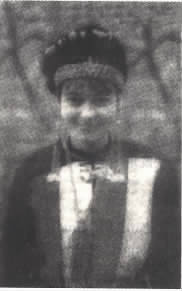
\includegraphics[width=0.3\linewidth]{picture/2002.png}
\end{figure}








\bta{2003}


\section{Use of English}

\noindent
\textbf{Directions:}\\
Read the following text. Choose the best word (s) for each
	numbered blank and mark A, B, C OR D on ANSWER SHEET 1. (10 points)

\TiGanSpace


Teachers need to be aware of the emotional, intellectual, and physical
changes that young adults experience. And they also need to give serious
\cloze to how they can best \cloze such changes. Growing
bodies need movement and \cloze , but not just in ways that
emphasize competition. \cloze they are adjusting to their new
bodies and a whole host of new intellectual and emotional challenges,
teenagers are especially self-conscious and need the \cloze that
comes from achieving success and knowing that their accomplishments are
\cloze by others. However, the typical teenage lifestyle is
already filled with so much competition that it would be \cloze
to plan activities in which there are more winners than losers,
\cloze , publishing newsletters with many student-written book
reviews, \cloze student artwork, and sponsoring book discussion
clubs. A variety of small clubs can provide \cloze opportunities
for leadership, as well as for practice in successful \cloze
dynamics. Making friends is extremely important to teenagers, and many
shy students need the \cloze of some kind of organization with a
supportive adult \cloze visible in the background.

In these activities, it is important to remember that the young teens
have \cloze attention spans. A variety of activities should be
organized \cloze participants can remain active as long as they
want and then go on to \cloze else without feeling guilty and
without letting the other participants \cloze. This does not
mean that adults must accept irresponsibility. \cloze they can
help students acquire a sense of commitment by \cloze for roles
that are within their \cloze and their attention spans and by
having clearly stated rules.


\newpage

\begin{enumerate}
	%\renewcommand{\labelenumi}{\arabic{enumi}.}
	% A(\Alph) a(\alph) I(\Roman) i(\roman) 1(\arabic)
	%设定全局标号series=example	%引用全局变量resume=example
	%[topsep=-0.3em,parsep=-0.3em,itemsep=-0.3em,partopsep=-0.3em]
	%可使用leftmargin调整列表环境左边的空白长度 [leftmargin=0em]
	\item
\fourchoices
{thought}
{idea}
{opinion}
{advice}




\item

\fourchoices
{strengthen}
{accommodate}
{stimulate}
{enhance}



\item


\fourchoices
{care}
{nutrition}
{exercise}
{leisure}




\item


\fourchoices
{If}
{Although}
{Whereas}
{Because}




\item

\fourchoices
{assistance}
{guidance}
{confidence}
{tolerance}



\item


\fourchoices
{claimed}
{admired}
{ignored}
{surpassed}




\item


\fourchoices
{improper}
{risky}
{fair}
{wise}




\item


\fourchoices
{in effect}
{as a result}
{for example}
{in a sense}





\item

\fourchoices
{displaying}
{describing}
{creating}
{exchanging}



\item


\fourchoices
{durable}
{excessive}
{surplus}
{multiple}




\item

\fourchoices
{group}
{individual}
{personnel}
{corporation}



\item


\fourchoices
{consent}
{insurance}
{admission}
{security}




\item

\fourchoices
{particularly}
{barely}
{definitely}
{rarely}



\item


\fourchoices
{similar}
{long}
{different}
{short}




\item


\fourchoices
{if only}
{now that}
{so that}
{even if}




\item

\fourchoices
{everything}
{anything}
{nothing}
{something}


\item


\fourchoices
{off}
{down}
{out}
{alone}




\item

\fourchoices
{On the contrary}
{On the average}
{On the whole}
{On the other hand}


\item


\fourchoices
{making}
{standing}
{planning}
{taking}




\item

\fourchoices
{capability}
{responsibility}
{proficiency}
{efficiency}

\end{enumerate}



\section{Reading Comprehension}

\noindent
\textbf{Part A}\\
\textbf{Directions:}\\
Read the following four texts. Answer the questions below each
	text by choosing A, B, C or
	D. Mark your answers
	on ANSWER SHEET 1. (40 points)

\newpage
\subsection{Text 1}


Wild Bill Donovan would have loved the Inter net. The American spymaster
who built the Office of Strategic Services in the World War \lmd{2} and later
laid the roots for the CIA was fascinated with information. Donovan
believed in using whatever tools came to hand in the ``great game'' of
espionage---spying as a ``profession.'' These days the Net, which has
already re-made such everyday pastimes as buying books and sending mail,
is reshaping Donovan's vocation as well.

The latest revolution isn't simply a matter of gentlemen reading other
gentlemen's e-mail. That kind of electronic spying has been going on for
decades. In the past three or four years, the World Wide Web has given
birth to a whole industry of point-and-click spying. The spooks call it
``open source intelligence,'' and as the Net grows, it is becoming
increasingly influential. In 1995 the CIA held a contest to see who
could compile the most data about Burundi. The winner, by a large
margin, was a tiny Virginia company called Open-Source Solutions, whose
clear advantage was its mastery of the electronic world.

Among the firms making the biggest splash in the new world is
Straitford, Inc. , a private intelligence-analysis firm based in Austin,
Texas. Straitford makes money by selling the results of spying (covering
nations from Chile to Russia) to corporations like energy-services firm
McDermott International. Many of its predictions are available online at \emph{www.straiford.com}.

Straiford president George Friedman says he sees the online world as a
kind of mutually reinforcing tool for both information collection and
distribution, a spymaster's dream. Last week his firm was busy vacuuming
up data bits from the far corners of the world and predicting a crisis
in Ukraine. ``As soon as that report runs, we'll suddenly get 500 new
internet sign-ups from Ukraine,'' says Friedman, a former political
science professor. ``And we'll hear back from some of them.''
Open-source spying does have its risks, of course, since it can be
difficult to tell good information from bad. That's where Straitford
earns its keep.

Friedman relies on a lean staff of 20 in Austin. Several of his staff
members have military-intelligence backgrounds. He sees the firm's
outsider status as the key to its success. Straitford's briefs don't
sound like the usual Washington back-and-forthing, whereby agencies
avoid dramatic declarations on the chance they might be wrong.
Straitford, says Friedman, takes pride in its independent voice.


\begin{enumerate}[resume]
	%\renewcommand{\labelenumi}{\arabic{enumi}.}
	% A(\Alph) a(\alph) I(\Roman) i(\roman) 1(\arabic)
	%设定全局标号series=example	%引用全局变量resume=example
	%[topsep=-0.3em,parsep=-0.3em,itemsep=-0.3em,partopsep=-0.3em]
	%可使用leftmargin调整列表环境左边的空白长度 [leftmargin=0em]
	\item
The emergence of the Net has \lineread.


\fourchoices
{received support from fans like Donovan}
{remolded the intelligence services}
{restored many common pastimes}
{revived spying as a profession}


\item
 Donovan's story is mentioned in the text to \lineread.

\fourchoices
{introduce the topic of online spying}
{show how he fought for the US}
{give an episode of the information war}
{honor his unique services to the CIA}


\item
The phrase ``making the biggest splash'' (line 1, paragraph 3) most
probably means \lineread.


\fourchoices
{causing the biggest trouble}
{exerting the greatest effort}
{achieving the greatest success}
{enjoying the widest popularity}



\item
 It can be learned from paragraph 4 that \lineread.

\fourchoices
{straitford's prediction about Ukraine has proved true}
{straitford guarantees the truthfulness of its information}
{straitford's business is characterized by unpredictability}
{straitford is able to provide fairly reliable information}


\item
Straitford is most proud of its \lineread.


\fourchoices
{official status}
{nonconformist image}
{efficient staff}
{military background}



\end{enumerate}


\newpage
\subsection{Text 2}


To paraphrase 18th-century statesman Edmund Burke,
``all that is needed for the triumph of a misguided cause is that good
people do nothing.'' One such cause now seeks to end biomedical research
because of the theory that animals have rights ruling out their use in
research. Scientists need to respond forcefully to animal rights
advocates, whose arguments are confusing the public and thereby
threatening advances in health knowledge and care. Leaders of the animal
rights movement target biomedical research because it depends on public
funding, and few people understand the process of health care research.
Hearing allegations of cruelty to animals in research settings, many are
perplexed that anyone would deliberately harm an animal.

For example, a grandmotherly woman staffing an animal rights booth at a
recent street fair was distributing a brochure that encouraged readers
not to use anything that comes from or is tested in animals---no meat,
no fur, no medicines. Asked if she opposed immunizations, she wanted to
know if vaccines come from animal research. When assured that they do,
she replied, ``Then I would have to say yes.'' Asked what will happen
when epidemics return, she said, ``Don't worry, scientists will find
some way of using computers.'' Such well-meaning people just don't
understand.

Scientists must communicate their message to the public in a
compassionate, understandable way---in human terms, not in the language
of molecular biology. We need to make clear the connection between
animal research and a grandmother's hip replacement, a father's bypass
operation, a baby's vaccinations, and even a pet's shots. To those who
are unaware that animal research was needed to produce these treatments,
as well as new treatments and vaccines, animal research seems wasteful
at best and cruel at worst.

Much can be done. Scientists could ``adopt'' middle school classes and
present their own research. They should be quick to respond to letters
to the editor, lest animal rights misinformation go unchallenged and
acquire a deceptive appearance of truth. Research institutions could be
opened to tours, to show that laboratory animals receive humane care.
Finally, because the ultimate stakeholders are patients, the health
research community should actively recruit to its cause not only
well-known personalities such as Stephen Cooper, who has made courageous
statements about the value of animal research, but all who receive
medical treatment. If good people do nothing, there is a real
possibility that an uninformed citizenry will extinguish the precious
embers of medical progress.


\begin{enumerate}[resume]
	%\renewcommand{\labelenumi}{\arabic{enumi}.}
	% A(\Alph) a(\alph) I(\Roman) i(\roman) 1(\arabic)
	%设定全局标号series=example	%引用全局变量resume=example
	%[topsep=-0.3em,parsep=-0.3em,itemsep=-0.3em,partopsep=-0.3em]
	%可使用leftmargin调整列表环境左边的空白长度 [leftmargin=0em]
	\item
 The author begins his article with Edmund Burke's words to \lineread.


\fourchoices
{call on scientists to take some actions}
{criticize the misguided cause of animal rights}
{warn of the doom of biomedical research}
{show the triumph of the animal rights movement}


\item
Misled people tend to think that using an animal in research is \lineread.


\fourchoices
{cruel but natural}
{inhuman and unacceptable}
{inevitable but vicious}
{pointless and wasteful}


\item
 The example of the grandmotherly woman is used to show the public's \lineread.


\fourchoices
{discontent with animal research}
{ignorance about medical science}
{indifference to epidemics}
{anxiety about animal rights}


\item
The author believes that, in face of the challenge from animal
rights advocates, scientists should \lineread.


\fourchoices
{communicate more with the public}
{employ hi-tech means in research}
{feel no shame for their cause}
{strive to develop new cures}


\item
From the text we learn that Stephen Cooper is \lineread.


\fourchoices
{a well-known humanist}
{a medical practitioner}
{an enthusiast in animal rights}
{a supporter of animal research}


\end{enumerate}



\newpage
\subsection{Text 3}


In recent years, railroads have been combining with each other, merging
into supersystems, causing heightened concerns about monopoly. As
recently as 1995, the top four railroads accounted for under 70 percent
of the total ton-miles moved by rails. Next year, after a series of
mergers is completed, just four railroads will control well over 90
percent of all the freight moved by major rail carriers.

Supporters of the new supersystems argue that these mergers will allow
for substantial cost reductions and better coordinated service. Any
threat of monopoly, they argue, is removed by fierce competition from
trucks. But many shippers complain that for heavy bulk commodities
traveling long distances, such as coal, chemicals, and grain, trucking
is too costly and the railroads therefore have them by the throat.

The vast consolidation within the rail industry means that most shippers
are served by only one rail company. Railroads typically charge
such``captive''shippers 20 to 30 percent more than they do when another
railroad is competing for the business. Shippers who feel they are being
overcharged have the right to appeal to the federal government's Surface
Transportation Board for rate relief, but the process is expensive, time
consuming, and will work only in truly extreme cases.

Railroads justify rate discrimination against captive shippers on the
grounds that in the long run it reduces everyone's cost. If railroads
charged all customers the same average rate, they argue, shippers who
have the option of switching to trucks or other forms of transportation
would do so, leaving remaining customers to shoulder the cost of keeping
up the line. It's theory to which many economists subscribe, but in
practice it often leaves railroads in the position of determining which
companies will flourish and which will fail. ``Do we really want
railroads to be the \uline{arbiters} of who wins and who loses in the
marketplace?''asks Martin Bercovici, a Washington lawyer who frequently
represents shipper.

Many captive shippers also worry they will soon be hit with a round of
huge rate increases. The railroad industry as a whole, despite its
brightening fortuning fortunes, still does not earn enough to cover the
cost of the capital it must invest to keep up with its surging traffic.
Yet railroads continue to borrow billions to acquire one another, with
Wall Street cheering them on. Consider the \$10.2 billion bid by Norfolk
Southern and CSX to acquire Conrail this year. Conrail's net railway
operating income in 1996 was just \$427 million, less than half of the
carrying costs of the transaction. Who's going to pay for the rest of
the bill? Many captive shippers fear that they will, as Norfolk Southern
and CSX increase their grip on the market.


\begin{enumerate}[resume]
	%\renewcommand{\labelenumi}{\arabic{enumi}.}
	% A(\Alph) a(\alph) I(\Roman) i(\roman) 1(\arabic)
	%设定全局标号series=example	%引用全局变量resume=example
	%[topsep=-0.3em,parsep=-0.3em,itemsep=-0.3em,partopsep=-0.3em]
	%可使用leftmargin调整列表环境左边的空白长度 [leftmargin=0em]
	\item
According to those who support mergers, railway monopoly is unlikely
because \lineread.


\fourchoices
{cost reduction is based on competition}
{services call for cross-trade coordination}
{outside competitors will continue to exist}
{shippers will have the railway by the throat}


\item
What is many captive shippers' attitude towards the consolidation in
the rail industry?


\fourchoices
{Indifferent.}
{Supportive.}
{Indignant.}
{Apprehensive.}


\item
 It can be inferred from paragraph 3 that \lineread.


\fourchoices
{shippers will be charged less without a rival railroad}
{there will soon be only one railroad company nationwide}
{overcharged shippers are unlikely to appeal for rate relief}
{a government board ensures fair play in railway business}

\item
The word ``arbiters''(line 7, paragraph 4) most probably refers to
those \lineread.


\fourchoices
{who work as coordinators}
{who function as judges}
{who supervise transactions}
{who determine the price}


\item
According to the text, the cost increase in the rail industry is
mainly caused by \lineread.


\fourchoices
{the continuing acquisition}
{the growing traffic}
{the cheering Wall Street}
{the shrinking market}


\end{enumerate}


\newpage
\subsection{Text 4}


It is said that in England death is pressing, in Canada inevitable and
in California optional. Small wonder. Americans' life expectancy has
nearly doubled over the past century. Failing hips can be replaced,
clinical depression controlled, cataracts removed in a 30-minute
surgical procedure. Such advances offer the aging population a quality
of life that was unimaginable when I entered medicine 50 years ago. But
not even a great health-care system can cure death---and our failure to
confront that reality now threatens this greatness of ours.

Death is normal; we are genetically programmed to disintegrate and
perish, even under ideal conditions. We all understand that at some
level, yet as medical consumers we treat death as a problem to be
solved. Shielded by third-party payers from the cost of our care, we
demand everything that can possibly be done for us, even if it's
useless. The most obvious example is late-stage cancer care.
Physicians---frustrated by their inability to cure the disease and
fearing loss of hope in the patient---too often offer aggressive
treatment far beyond what is scientifically justified.

In 1950, the US spent \$12.7 billion on health care. In 2002, the cost
will be \$1,540 billion. Anyone can see this trend is unsustainable. Yet
few seem willing to try to reverse it. Some scholars conclude that a
government with finite resources should simply stop paying for medical
care that sustains life beyond a certain age---say 83 or so. Former
Colorado governor Richard Lamm has been quoted as saying that the old
and infirm ``have a duty to die and get out of the way'', so that
younger, healthier people can realize their potential.

I would not go that far. Energetic people now routinely work through
their 60s and beyond, and remain dazzlingly productive. At 78, Viacom
chairman Sumner Redstone jokingly claims to be 53. Supreme Court Justice
Sandra Day O'Connor is in her 70 s, and former surgeon general
C. Everett
Koop chairs an Internet start-up in his 80 s. These leaders are living
proof that prevention works and that we can manage the health problems
that come naturally with age. As a mere 68-year-old, I wish to age as
productively as they have.

Yet there are limits to what a society can spend in this pursuit. As a
physician, I know the most costly and dramatic measures may be
ineffective and painful. I also know that people in Japan and Sweden,
countries that spend far less on medical care, have achieved longer,
healthier lives than we have. As a nation, we may be overfunding the
quest for unlikely cures while underfunding research on humbler
therapies that could improve people's lives.


\begin{enumerate}[resume]
	%\renewcommand{\labelenumi}{\arabic{enumi}.}
	% A(\Alph) a(\alph) I(\Roman) i(\roman) 1(\arabic)
	%设定全局标号series=example	%引用全局变量resume=example
	%[topsep=-0.3em,parsep=-0.3em,itemsep=-0.3em,partopsep=-0.3em]
	%可使用leftmargin调整列表环境左边的空白长度 [leftmargin=0em]
	\item
 What is implied in the first sentence?

\fourchoices
{Americans are better prepared for death than other people.}
{Americans enjoy a higher life quality than ever before.}
{Americans are over-confident of their medical technology.}
{Americans take a vain pride in their long life expectancy.}


\item
The author uses the example of caner patients to show that \lineread.


\fourchoices
{medical resources are often wasted}
{doctors are helpless against fatal diseases}
{some treatments are too aggressive}
{medical costs are becoming unaffordable}


\item
The author's attitude toward Richard Lamm's remark is one of \lineread.


\fourchoices
{strong disapproval}
{reserved consent}
{slight contempt}
{enthusiastic support}



\item
 In contras to the US, Japan and Sweden are funding their medical
care \lineread.


\fourchoices
{more flexibly}
{more extravagantly}
{more cautiously}
{more reasonably}


\item
The text intends to express the idea that \lineread.


\fourchoices
{medicine will further prolong people's lives}
{life beyond a certain limit is not worth living}
{death should be accepted as a fact of life}
{excessive demands increase the cost of health care}


\end{enumerate}



\newpage

\noindent
\textbf{Part B}\\
\textbf{Directions:}\\
{Read the following text carefully and then translate the
	underlined segments into Chinese. Your translation should be written
	clearly on ANSWER SHEET 2. (10 points)


\TiGanSpace



Human beings in all times and places think about their world and wonder
at their place in it. Humans are thoughtful and creative, possessed of
insatiable curiosity. \transnum \uline{Furthermore, humans have the
	ability to modify the environment in which they live, thus subjecting
	all other life forms to their own peculiar ideas and fancies.}
Therefore, it is important to study humans in all their richness and
diversity in a calm and systematic manner, with the hope that the
knowledge resulting from such studies can lead humans to a more
harmonious way of living with themselves and with all other life forms
on this planet Earth.

``Anthropology'' derives from the Greek words \emph{anthropos} ``human''
and \emph{logos} ``the study of.'' By its very name, anthropology
encompasses the study of all humankind.

Anthropology is one of the social sciences. \transnum \uline{Social
	science is that branch of intellectual enquiry which seeks to study
	humans and their endeavors in the same reasoned, orderly, systematic,
	and dispassioned manner that natural scientists use for the study of
	natural phenomena}.

Social science disciplines include geography, economics, political,
science, psychology, and sociology. Each of these social sciences has a
subfield or specialization which lies particularly close to
anthropology.

All the social sciences focus upon the study of humanity. Anthropology
is a field-study oriented discipline which makes extensive use of the
comparative method in analysis. \transnum \uline{The emphasis on data
	gathered first-hand, combined with a cross-cultural perspective brought
	to the analysis of cultures past and present, makes this study a unique
	and distinctly important social science}.

Anthropological analyses rest heavily upon the concept of culture. Sir
Edward Tylor's formulation of the concept of culture was one of the
great intellectual achievements of 19th century
science. \transnum \uline{Tylor defined culture as ``\ldots that complex
	whole which includes belief, art, morals, law, custom, and any other
	capabilities and habits acquired by man as a member of society.''} This
insight, so profound in its simplicity, opened up an entirely new way of
perceiving and understanding human life. Implicit within Tylor's
definition is the concept that culture is learned. shared, and patterned
behavior.

 \transnum \uline{Thus, the anthropological concept of ``culture,'' like
	the concept of ``set'' in mathematics, is an abstract concept which
	makes possible immense amounts of concrete research and understanding.}



\section{Writing}




\noindent
\textbf{46. Directions}

Study the following set of drawings carefully and write an essay
entitled in which you should
\begin{listwrite}
\item 
describe the set of drawings, interpret its meaning, and

\item 
point out its implications in our life.
\end{listwrite}


You should write about 200 words neatly on ANSWER SHEET 2. (20 points)


\begin{figure}[h!]
	\centering
	\includesvg[width=0.67\linewidth]{picture/svg/picture-02}
	\caption*{温室花朵经不起风雨}
\end{figure}





\bta{2004}


\section{Use of English}

\noindent
\textbf{Directions:}\\
Read the following text. Choose the best word (s) for each numbered blank
and mark A, B, C or D on ANSWER SHEET 1. (10 points)


\TiGanSpace


Many theories concerning the causes of juvenile delinquency (crimes
committed by young people) focus either on the individual or on society
as the major contributing influence. Theories \cloze on the
individual suggest that children engage in criminal behavior
\cloze they were not sufficiently penalized for previous misdeeds
or that they have learned criminal behavior through \cloze with
others. Theories focusing on the role of society suggest that children
commit crimes in \cloze to their failure to rise above their
socioeconomic status, \cloze as a rejection of middle-class
values.

Most theories of juvenile delinquency have focused on children from
disadvantaged families, \cloze the fact that children from
wealthy homes also commit crimes. The latter may commit crimes
\cloze lack of adequate parental control. All theories, however,
are tentative and are \cloze to criticism.

Changes in the social structure may indirectly \cloze juvenile
crime rates. For example, changes in the economy that \cloze to
fewer job opportunities for youth and rising unemployment \cloze
make gainful employment increasingly difficult to obtain. The resulting
discontent may in \cloze lead more youths into criminal
behavior.

Families have also \cloze changes these years. More families
consist of one-parent households or two working parents; \cloze , children are likely to have less supervision at home \cloze
was common in the traditional family \cloze. This lack of
parental supervision is thought to be an influence on juvenile crime
rates. Other \cloze causes of offensive acts include
frustration or failure in school, the increased \cloze
of drugs and alcohol, and the growing \cloze of child abuse and
child neglect. All these conditions tend to increase the probability of
a child committing a criminal act, \cloze a direct causal
relationship has not yet been established.


\newpage
\begin{enumerate}
	%\renewcommand{\labelenumi}{\arabic{enumi}.}
	% A(\Alph) a(\alph) I(\Roman) i(\roman) 1(\arabic)
	%设定全局标号series=example	%引用全局变量resume=example
	%[topsep=-0.3em,parsep=-0.3em,itemsep=-0.3em,partopsep=-0.3em]
	%可使用leftmargin调整列表环境左边的空白长度 [leftmargin=0em]
	\item


\fourchoices
{acting}
{relying}
{centering}
{commenting}




\item


\fourchoices
{before}
{unless}
{until}
{because}




\item

\fourchoices
{interaction}
{assimilation}
{cooperation}
{consultation}


\item


\fourchoices
{return}
{reply}
{reference}
{response}




\item
\fourchoices
{or}
{but rather}
{but}
{or else}



\item

\fourchoices
{considering}
{ignoring}
{highlighting}
{discarding}



\item


\fourchoices
{on}
{in}
{for}
{with}




\item


\fourchoices
{immune}
{resistant}
{sensitive}
{subject}




\item


\fourchoices
{affect}
{reduce}
{chock}
{reflect}




\item


\fourchoices
{point}
{lead}
{come}
{amount}




\item


\fourchoices
{in general}
{on average}
{by contrast}
{at length}





\item


\fourchoices
{case}
{short}
{turn}
{essence}




\item

\fourchoices
{survived}
{noticed}
{undertaken}
{experienced}



\item

\fourchoices
{contrarily}
{consequently}
{similarly}
{simultaneously}


\item


\fourchoices
{than}
{that}
{which}
{as}




\item


\fourchoices
{system}
{structure}
{concept}
{heritage}




\item

\fourchoices
{assessable}
{identifiable}
{negligible}
{incredible}


\item

\fourchoices
{expense}
{restriction}
{allocation}
{availability}



\item

\fourchoices
{incidence}
{awareness}
{exposure}
{popularity}



\item


\fourchoices
{provided}
{since}
{although}
{supposing}



\end{enumerate}


\hfil

\section{Reading Comprehension}



\noindent
\textbf{Part A}\\
\textbf{Directions:}\\
Read the following four texts. Answer the questions below each
	text by choosing A, B, C or
	D. Mark your answers
	on ANSWER SHEET 1. (40 points)

\newpage
\subsection{Text 1}


Hunting for a job late last year, lawyer Gant Redmon stumbled across
CareerBuilder, a job database on the Internet. He searched it with no
success but was attracted by the site's ``personal search agent''. It's
an interactive feature that lets visitors key in job criteria such as
location, title, and salary, then E-mails them when a matching position
is posted in the database. Redmon chose the keywords \emph{legal},
	\emph{intellectual property} and \emph{Washington, D.C.} Three weeks later, he
got his first notification of an opening. ``I struck gold,'' says
Redmon, who E-mailed his resume to the employer and won a position as
in-house counsel for a company.

With thousands of career-related sites on the Internet, finding
promising openings can he time-consuming and inefficient. Search agents
reduce the need for repeated visits to the databases. But although a
search agent worked for Redmon, career experts see drawbacks. Narrowing
your criteria, for example, may work against you: ``Every time you
answer a question you eliminate a possibility,'' says one expert.

For any job search, you should start with a narrow concept---what you
think you want to do---then broaden it. ``None of these programs do
that,'' says another expert. ``There's no career counseling implicit in
all of this.'' Instead, the best strategy is to use the agent as a kind
of \uline{tip service} to keep abreast of jobs in a particular
database; when you get E-mail, consider it a reminder to check the
database again. ``I would not rely on agents for finding everything that
is added to a database that might interest me,'' says the author of a
job-searching guide.

Some sites design their agents to tempt job hunters to return. When
CareerSite's agent sends out messages to those who have signed up for
its service, for example, it includes only three potential jobs---those
it considers the best matches. There may be more matches in the
database; job hunters will have to visit the site again to find
them---and they do. ``On the day after we send our messages, we see a
sharp increase in our traffic,'' says Seth Peets, vice president of
marketing for CareerSite.

Even those who aren't hunting for jobs may find search agents
worthwhile. Some use them to keep a close watch on the demand for their
line of work or gather information on compensation to arm themselves
when negotiating for a raise. Although happily employed, Redmon
maintains his agent at CareerBuilder. ``You always keep your eyes
open,'' he says. Working with a personal search agent means having
another set of eyes looking out for you.


\begin{enumerate}[resume]
	%\renewcommand{\labelenumi}{\arabic{enumi}.}
	% A(\Alph) a(\alph) I(\Roman) i(\roman) 1(\arabic)
	%设定全局标号series=example	%引用全局变量resume=example
	%[topsep=-0.3em,parsep=-0.3em,itemsep=-0.3em,partopsep=-0.3em]
	%可使用leftmargin调整列表环境左边的空白长度 [leftmargin=0em]
	\item
How did Redmon find his job?


\fourchoices
{By searching openings in a job database.}
{By posting a matching position in a database.}
{By using a special service of a database.}
{By E-mailing his resume to a database.}


\item
Which of the following can be a disadvantage of search agents?


\fourchoices
{Lack of counseling.}
{Limited number of visits.}
{Lower efficiency.}
{Fewer successful matches.}


\item
The expression ``tip service'' (Line 4, Paragraph 3) most probably
means \lineread.


\fourchoices
{advisory}
{compensation}
{interaction}
{reminder}


\item
Why does CareerSite's agent offer each job hunter only three job
options?


\fourchoices
{To focus on better job matches.}
{To attract more returning visits.}
{To reserve space for more messages.}
{To increase the rate of success.}


\item
Which of the following is true according to the text?

\fourchoices
{Personal search agents are indispensable to job-hunters.}
{Some sites keep E-mailing job seekers to trace their demands.}
{Personal search agents are also helpful to those already}
{Some agents stop sending information to people once they are}


\end{enumerate}

	
\newpage
\subsection{Text 2}
	


Over the past century, all kinds of unfairness and discrimination have
been condemned or made illegal. But one insidious form continues to
thrive: alphabetism. This, for those as yet unaware of such a
disadvantage, refers to discrimination against those whose surnames
begin with a letter in the lower half of the alphabet.

It has long been known that a taxi firm called AAAA cars has a big
advantage over Zodiac cars when customers thumb through their phone
directories. Less well known is the advantage that Adam Abbott has in
life over Zoë Zysman. English names are fairly evenly spread between the
halves of the alphabet. Yet a suspiciously large number of top people
have surnames beginning with letters between A and K.

Thus the American president and vice-president have surnames starting
with B and C respectively; and 26 of George Bush's predecessors
(including his father) had surnames in the first half of the alphabet
against just 16 in the second half. Even more striking, six of the seven
heads of government of the G 7 rich countries are alphabetically
advantaged (Berlusconi, Blair, Bush, Chirac, Chrétien and Koizumi). The
world's three top central bankers (Greenspan, Duisenberg and Hayami) are
all close to the top of the alphabet, even if one of them really uses
Japanese characters. As are the world's five richest men (Gates,
Buffett, Allen, Ellison and Albrecht).

Can this merely be coincidence? One theory, dreamt up in all the spare
time enjoyed by the alphabetically disadvantaged, is that the rot sets
in early. At the start of the first year in infant school, teachers seat
pupils alphabetically from the front, to make it easier to remember
their names. So short-sighted Zysman junior gets stuck in the back row,
and is rarely asked the improving questions posed by those insensitive
teachers. At the time the alphabetically disadvantaged may think they
have had a lucky escape. Yet the result may be worse qualifications,
because they get less individual attention, as well as less confidence
in speaking publicly.

The humiliation continues. At university graduation ceremonies, the ABCs
proudly get their awards first; by the time they reach the Zysmans \uline{most
people are literally having a ZZZ}. Shortlists for job interviews,
election ballot papers, lists of conference speakers and attendees: all
tend to be drawn up alphabetically, and their recipients lose interest
as they plough through them.

\newpage
\begin{enumerate}[resume]
	%\renewcommand{\labelenumi}{\arabic{enumi}.}
	% A(\Alph) a(\alph) I(\Roman) i(\roman) 1(\arabic)
	%设定全局标号series=example	%引用全局变量resume=example
	%[topsep=-0.3em,parsep=-0.3em,itemsep=-0.3em,partopsep=-0.3em]
	%可使用leftmargin调整列表环境左边的空白长度 [leftmargin=0em]
	\item
What does the author intend to illustrate with AAAA cars and Zodiac
cars?


\fourchoices
{A kind of overlooked inequality.}
{A type of conspicuous bias.}
{A type of personal prejudice.}
{A kind of brand discrimination.}

 
\item
 What can we infer from the first three paragraphs?

\fourchoices
{In both East and West, names are essential to success.}
{The alphabet is to blame for the failure of Zoë Zysman.}
{Customers often pay a lot of attention to companies' names.}
{Some form of discrimination is too subtle to recognize.}



\item
The 4th paragraph suggests that \lineread.

\fourchoices
{questions are often put to the more intelligent students}
{alphabetically disadvantaged students often escape from class}
{teachers should pay attention to all of their students}
{students should be seated according to their eyesight}


\item
What does the author mean by ``most people are literally having a
ZZZ'' (Lines 2$ \sim $3, Paragraph 5)?


\fourchoices
{They are getting impatient.}
{They are noisily dozing off.}
{They are feeling humiliated.}
{They are busy with word puzzles.}


\item
Which of the following is true according to the text?

\fourchoices
{People with surnames beginning with N to Z are often ill-treated.}
{VIPs in the Western world gain a great deal from alphabetism.}
{The campaign to eliminate alphabetism still has a long way to go.}
{Putting things alphabetically may lead to unintentional bias.}

\end{enumerate}


\newpage
\subsection{Text 3}



When it comes to the slowing economy, \uline{Ellen Spero isn't biting her nails
just yet}. But the 47-year-old manicurist isn't cutting, filing or
polishing as many nails as she'd like to, either. Most of her clients
spend \$12 to \$50 weekly, but last month two longtime customers
suddenly stopped showing up. Spero blames the softening economy. ``I'm a
good economic indicator,'' she says. ``I provide a service that people
can do without when they're concerned about saving some dollars.'' So
Spero is downscaling, shopping at middle-brow Dillard's department store
near her suburban Cleveland home, instead of Neiman Marcus. ``I don't
know if other clients are going to abandon me, too,'' she says.

Even before Alan Greenspan's admission that America's red-hot economy is
cooling, lots of working folks had already seen signs of the slowdown
themselves. From car dealerships to Gap outlets, sales have been lagging
for months as shoppers temper their spending. For retailers, who last
year took in 24 percent of their revenue between Thanksgiving and
Christmas, the cautious approach is coming at a crucial time. Already,
experts say, holiday sales are off 7 percent from last year's pace. But
don't sound any alarms just yet. Consumers seem only mildly concerned,
not panicked, and many say they remain optimistic about the economy's
long-term prospects even as they do some modest belt-tightening.

Consumers say they're not in despair because, despite the dreadful
headlines, their own fortunes still feel pretty good. Home prices are
holding steady in most regions. In Manhattan, ``there's a new gold rush
happening in \uline{the \$4 million to \$10 million range}, predominantly fed by
Wall Street bonuses,'' says broker Barbara Corcoran. In San Francisco,
prices are still rising even as frenzied overbidding quiets. ``Instead
of 20 to 30 offers, now maybe you only get two or three," says John
Tealdi, a Bay Area real-estate broker. And most folks still feel pretty
comfortable about their ability to find and keep a job.

Many folks see silver linings to this slowdown. Potential home buyers
would cheer for lower interest rates. Employers wouldn't mind a little
fewer bubbles in the job market. Many consumers seem to have been
influenced by stock-market swings, which investors now view as a
necessary ingredient to a sustained boom. Diners might see an upside,
too. Getting a table at Manhattan's hot new Alain Ducasse restaurant
used to be impossible. Not anymore. For that, Greenspan \& Co. may still
be worth toasting.

\begin{enumerate}[resume]
	%\renewcommand{\labelenumi}{\arabic{enumi}.}
	% A(\Alph) a(\alph) I(\Roman) i(\roman) 1(\arabic)
	%设定全局标号series=example	%引用全局变量resume=example
	%[topsep=-0.3em,parsep=-0.3em,itemsep=-0.3em,partopsep=-0.3em]
	%可使用leftmargin调整列表环境左边的空白长度 [leftmargin=0em]
	\item
By ``Ellen Spero isn't biting her nails just yet'' (Line 1,
Paragraph 1), the author means \lineread.


\fourchoices
{Spero can hardly maintain her business}
{Spero is too much engaged in her work}
{Spero has grown out of her bad habit}
{Spero is not in a desperate situation}


\item
How do the public feel about the current economic situation?


\fourchoices
{Optimistic.}
{Confused.}
{Carefree.}
{Panicked.}


\item
 When mentioning ``the \$4 million to \$10 million range'' (Lines 3,
Paragraph 3), the author is talking about \lineread.

\fourchoices
{gold market}
{real estate}
{stock exchange}
{venture investment}


\item
Why can many people see ``silver linings'' to the economic slowdown?


\fourchoices
{They would benefit in certain ways.}
{The stock market shows signs of recovery.}
{Such a slowdown usually precedes a boom.}
{The purchasing power would be enhanced.}


\item
To which of the following is the author likely to agree?


\fourchoices
{A new boom, on the horizon.}
{Tighten the belt, the single remedy.}
{Caution all right, panic not.}
{The more ventures, the more chances.}



\end{enumerate}


\newpage
\subsection{Text 4}


Americans today don't place a very high value on intellect. Our heroes
are athletes, entertainers, and entrepreneurs, not scholars. Even our
schools are where we send our children to get a practical
education---not to pursue knowledge for the sake of knowledge. Symptoms
of pervasive anti-intellectualism in our schools aren't difficult to
find.

``Schools have always been in a society where practical is more
important than intellectual,'' says education writer Diane Ravitch.
``Schools could be a counterbalance.'' Ravitch's latest book. \emph{Left
	Back: A Century of Failed School Reforms}, traces the roots of
anti-intellectualism in our schools, concluding they are anything but a
counterbalance to the American distaste for intellectual pursuits.

But they could and should be. Encouraging kids to reject the life of the
mind leaves them vulnerable to exploitation and control. Without the
ability to think critically, to defend their ideas and understand the
ideas of others, they cannot fully participate in our democracy.
Continuing along this path, says writer Earl Shorris, ``We will become a
second-rate country. We will have a less civil society.''

``Intellect is resented as a form of power or privilege,'' writes
historian and professor Richard Hofstadter in \emph{Anti-intellectualism
	in American Life,} a Pulitzer-Prize winning book on the roots of
anti-intellectualism in US politics, religion, and education. From the
beginning of our history, says Hofstadter, our democratic and populist
urges have driven us to reject anything that smells of elitism.
Practicality, common sense, and native intelligence have been considered
more noble qualities than anything you could learn from a book.

Ralph Waldo Emerson and other Transcendentalist philosophers thought
schooling and rigorous book learning put unnatural restraints on
children: ``We are shut up in schools and college recitation rooms for
10 or 15 years and come out at last with a bellyful of words and do not
know a thing.''Mark Twain's \emph{Huckleberry Finn} exemplified American
anti-intellectualism. Its hero avoids being civilized---going to school
and learning to read---so he can preserve his innate goodness.

Intellect, according to Hofstadter, is different from native
intelligence, a quality we reluctantly admire. Intellect is the
critical, creative, and contemplative side of the mind. Intelligence
seeks to grasp, manipulate, re-order, and adjust, while intellect
examines, ponders, wonders, theorizes, criticizes, and imagines.

School remains a place where intellect is mistrusted. Hofstadter says
our country's educational system is in the grips of people who
``joyfully and militantly proclaim their hostility to intellect and
their eagerness to identify with children who show the least
intellectual promise.''


\begin{enumerate}[resume]
	%\renewcommand{\labelenumi}{\arabic{enumi}.}
	% A(\Alph) a(\alph) I(\Roman) i(\roman) 1(\arabic)
	%设定全局标号series=example	%引用全局变量resume=example
	%[topsep=-0.3em,parsep=-0.3em,itemsep=-0.3em,partopsep=-0.3em]
	%可使用leftmargin调整列表环境左边的空白长度 [leftmargin=0em]
	\item
 What do American parents expect their children to acquire in school?


\fourchoices
{The habit of thinking independently.}
{Profound knowledge of the world.}
{Practical abilities for future career.}
{The confidence in intellectual pursuits.}


\item
We can learn from the text that Americans have a history
of \lineread.


\fourchoices
{undervaluing intellect}
{favoring intellectualism}
{supporting school reform}
{suppressing native intelligence}


\item
The views of Raviteh and Emerson on schooling are \lineread.


\fourchoices
{identical}
{similar}
{complementary}
{opposite}


\item
Emerson, according to the text, is probably \lineread.


\fourchoices
{a pioneer of education reform}
{an opponent of intellectualism}
{a scholar in favor of intellect}
{an advocate of regular schooling}



\item
What does the author think of intellect?


\fourchoices
{It is second to intelligence.}
{It evolves from common sense.}
{It is to be pursued.}
{It underlies power}


\end{enumerate}


\newpage

\noindent
\textbf{Part B}\\
\textbf{Directions:}\\
Read the following text carefully and then translate the
	underlined segments into Chinese. Your translation should be written
	clearly on ANSWER SHEET 2. (10 points)


\TiGanSpace


The relation of language and mind has interested philosophers for many
centuries. \transnum \uline{The Greeks assumed that the structure of
	language had some connection with the process of thought, which took
	root in Europe long before people realized how diverse languages could
	be.}

Only recently did linguists begin the serious study of languages that
were very different from their own. Two anthropologist-linguists, Franz
Boas and Edward Sapir, were pioneers in describing many native languages
of North and South America during the first half of the twentieth
century. \transnum \uline{We are obliged to them because some of these
	languages have since vanished, as the peoples who spoke them died out or
	became assimilated and lost their native languages.} Other linguists in
the earlier part of this century, however, who were less eager to deal
with bizarre data from ``exotic'' language, were not always so grateful.
\transnum \uline{The newly described languages were often so strikingly
	different from the well studied languages of Europe and Southeast Asia
	that some scholars even accused Boas and Sapir of fabricating their
	data.} Native American languages are indeed different, so much so in
fact that Navajo could be used by the US military as a code during World
War II to send secret messages.

Sapir's pupil, Benjamin Lee Whorf, continued the study of American
Indian languages. \transnum \uline{Being interested in the relationship
	of language and thought, Whorf developed the idea that the structure of
	language determines the structure of habitual thought in a society}. He
reasoned that because it is easier to formulate certain concepts and not
others in a given language, the speakers of that language think along
one track and not along another. \transnum \uline{Whorf came to believe
	in a sort of linguistic determinism which, in its strongest form, states
	that language imprisons the mind, and that the grammatical patterns in a
	language can produce far-reaching consequences for the culture of a
	society}. Later, this idea became to be known as the Sapir-Whorf
hypothesis, but this term is somewhat inappropriate. Although both Sapir
and Whorf emphasized the diversity of languages, Sapir himself never
explicitly supported the notion of linguistic determinism.



\section{Writing}


\textbf{46. Directions:}

Study the following drawing carefully and write an essay in
	which you should
\begin{listwrite}
\item 
 describe the drawing,



\item
 interpret its meaning, and



\item
support your view with examples.
\end{listwrite}

You should write about 200 words neatly on ANSWER SHEET 2. (20 points)


\begin{figure}[h!]
	\centering
	\includesvg[width=0.5\linewidth]{picture/svg/picture-03}
	\caption*{终点又是新起点}
\end{figure}




\bta{2005}




\section{Use of English}

\noindent
\textbf{Directions:}\\
{Read the following text. Choose the best word (s) for each
	numbered blank and mark A, B, C or D on ANSWER
	SHEET 1. (10 points)


\TiGanSpace


The human nose is an underrated tool. Humans are often thought to be
insensitive smellers compared with animals, \cloze this is
largely because, \cloze animals, we stand upright. This means that
our noses are \cloze to perceiving those smells which float
through the air, \cloze the majority of smells which stick to
surfaces. In fact, \cloze , we are extremely sensitive to
smells, \cloze we do not generally realize it. Our noses are
capable of \cloze human smells even when these
are \cloze to far below one part in one million.

Strangely, some people find that they can smell one type of flower but
not another, \cloze others are sensitive to the smells of both
flowers. This may be because some people do not have the genes necessary
to generate \cloze smell receptors in the nose. These receptors
are the cells which sense smells and send \cloze to the brain.
However, it has been found that even people insensitive to a certain
smell \cloze can suddenly become sensitive to it
when \cloze to it often enough.

The explanation for insensitivity to smell seems to be that brain finds
it \cloze to keep all smell receptors working all the time but
can \cloze new receptors if necessary. This
may \cloze explain why we are not usually sensitive to our own
smells---we simply do not need to be. We are not \cloze of the
usual smell of our own house, but we \cloze new smells when we
visit someone else's. The brain finds it best to keep smell
receptors \cloze for unfamiliar and emergency
signals \cloze the smell of smoke, which might indicate the
danger of fire.


\newpage

\begin{enumerate}
	%\renewcommand{\labelenumi}{\arabic{enumi}.}
	% A(\Alph) a(\alph) I(\Roman) i(\roman) 1(\arabic)
	%设定全局标号series=example	%引用全局变量resume=example
	%[topsep=-0.3em,parsep=-0.3em,itemsep=-0.3em,partopsep=-0.3em]
	%可使用leftmargin调整列表环境左边的空白长度 [leftmargin=0em]
	\item


\fourchoices
{although}
{as}
{but}
{while}




\item


\fourchoices
{above}
{unlike}
{excluding}
{besides}




\item


\fourchoices
{limited}
{committed}
{dedicated}
{confined}




\item


\fourchoices
{catching}
{ignoring}
{missing}
{tracking}




\item


\fourchoices
{anyway}
{though}
{instead}
{therefore}




\item


\fourchoices
{even if}
{if only}
{only if}
{as if}




\item

\fourchoices
{distinguishing}
{discovering}
{determining}
{detecting}


\item


\fourchoices
{diluted}
{dissolved}
{dispersed}
{diffused}




\item


\fourchoices
{when}
{since}
{for}
{whereas}




\item


\fourchoices
{unusual}
{particular}
{unique}
{typical}




\item


\fourchoices
{signs}
{stimuli}
{messages}
{impulses}




\item


\fourchoices
{at first}
{at all}
{at large}
{at times}




\item


\fourchoices
{subjected}
{left}
{drawn}
{exposed}




\item

\fourchoices
{ineffective}
{incompetent}
{inefficient}
{insufficient}


\item


\fourchoices
{introduce}
{summon}
{trigger}
{create}




\item


\fourchoices
{still}
{also}
{otherwise}
{nevertheless}




\item


\fourchoices
{sure}
{sick}
{aware}
{tired}




\item


\fourchoices
{tolerate}
{repel}
{neglect}
{notice}




\item

\fourchoices
{available}
{reliable}
{identifiable}
{suitable}


\item


\fourchoices
{similar to}
{such as}
{along with}
{aside from}



\end{enumerate}

\vfil

\section{Reading Comprehension}


\noindent
\textbf{Part A}\\
\textbf{Directions:}\\
Read the following four texts. Answer the questions below each
	text by choosing A, B, C or
	D. Mark your answers
	on ANSWER SHEET 1. (40 points)

\newpage
\subsection{Text 1}


Everybody loves a fat pay rise. Yet pleasure at your own can vanish if
you learn that a colleague has been given a bigger one. Indeed, if he
has a reputation for slacking, you might even be outraged. Such
behaviour is regarded as ``all too human'', with the underlying
assumption that other animals would not be capable of this finely
developed sense of grievance. But a study by Sarah Brosnan and Frans de
Waal of Emory University in Atlanta, Georgia, which has just been
published in \emph{Nature}, suggests that  \emph{it is all too monkey}, as well.

The researchers studied the behaviour of female brown capuchin monkeys.
They look cute. They are good-natured, co-operative creatures, and they
share their food readily. Above all, like their female human
counterparts, they tend to pay much closer attention to the value of
``goods and services'' than males.

Such characteristics make them perfect candidates for Dr. Brosnan's and
Dr. de Waal's study. The researchers spent two years teaching their
monkeys to exchange tokens for food. Normally, the monkeys were happy
enough to exchange pieces of rock for slices of cucumber. However, when
two monkeys were placed in separate but adjoining chambers, so that each
could observe what the other was getting in return for its rock, their
behaviour became markedly different.

In the world of capuchins grapes are luxury goods (and much preferable
to cucumbers). So when one monkey was handed a grape in exchange for her
token, the second was reluctant to hand hers over for a mere piece of
cucumber. And if one received a grape without having to provide her
token in exchange at all, the other either tossed her own token at the
researcher or out of the chamber, or refused to accept the slice of
cucumber. Indeed, the mere presence of a grape in the other chamber
(without an actual monkey to eat it) was enough to induce resentment in
a female capuchin.

The researchers suggest that capuchin monkeys, like humans, are guided
by social emotions. In the wild, they are a co-operative, group-living
species. Such co-operation is likely to be stable only when each animal
feels it is not being cheated. Feelings of righteous indignation, it
seems, are not the preserve of people alone. Refusing a lesser reward
completely makes these feelings abundantly clear to other members of the
group. However, whether such a sense of fairness evolved independently
in capuchins and humans, or whether it stems from the common ancestor
that the species had 35 million years ago, is, as yet, an unanswered
question.

\begin{enumerate}[resume]
	%\renewcommand{\labelenumi}{\arabic{enumi}.}
	% A(\Alph) a(\alph) I(\Roman) i(\roman) 1(\arabic)
	%设定全局标号series=example	%引用全局变量resume=example
	%[topsep=-0.3em,parsep=-0.3em,itemsep=-0.3em,partopsep=-0.3em]
	%可使用leftmargin调整列表环境左边的空白长度 [leftmargin=0em]
	\item
In the opening paragraph, the author introduces his topic by \lineread.


\fourchoices
{posing a contrast}
{justifying an assumption}
{making a comparison}
{explaining a phenomenon}


\item
The statement ``it is all too monkey'' (Last line, Paragraph
l) implies that \lineread.


\fourchoices
{monkeys are also outraged by slack rivals}
{resenting unfairness is also monkeys' nature}
{monkeys, like humans, tend to be jealous of each other}
{no animals other than monkeys can develop such emotions}


\item
Female capuchin monkeys were chosen for the research most
probably because they are \lineread.


\fourchoices
{more inclined to weigh what they get}
{attentive to researchers' instructions}
{nice in both appearance and temperament}
{more generous than their male companions}



\item
Dr. Brosnan and Dr. de Waal have eventually found in their
study that the monkeys \lineread.


\fourchoices
{prefer grapes to cucumbers}
{can be taught to exchange things}
{will not be co-operative if feeling cheated}
{are unhappy when separated from others}


\item
What can we infer from the last paragraph?


\fourchoices
{Monkeys can be trained to develop social emotions.}
{Human indignation evolved from an uncertain source.}
{Animals usually show their feelings openly as humans do.}
{Cooperation among monkeys remains stable only in the wild.}

	
\end{enumerate}


\newpage
\subsection{Text 2}


Do you remember all those years when scientists argued that smoking
would kill us but the doubters insisted that we didn't know for sure?
That the evidence was inconclusive, the science uncertain? That the
antismoking lobby was out to destroy our way of life and the government
should stay out of the way? Lots of Americans bought that nonsense, and
over three decades, some 10 million smokers went to early graves.

There are upsetting parallels today, as scientists in one wave after
another try to awaken us to the growing threat of global warming. The
latest was a panel from the National Academy of Sciences, enlisted by
the White House, to tell us that the Earth's atmosphere is definitely
warming and that the problem is largely man-made. The clear message is
that we should get moving to protect ourselves. The president of the
National Academy, Bruce Alberts, added this key point in the preface to
the panel's report: ``Science never has all the answers. But science
does provide us with the best available guide to the future, and it is
critical that our nation and the world base important policies on the
best judgments that science can provide concerning the future
consequences of present actions.''

Just as on smoking, voices now come from many quarters insisting that
the science about global warming is incomplete, that it's OK to keep
pouring fumes into the air until we know for sure. This is a dangerous
game: by the time 100 percent of the evidence is in, it may be too late.
With the risks obvious and growing, a prudent people would take out an
insurance policy now.

Fortunately, the White House is starting to pay attention. But it's
obvious that a majority of the president's advisers still don't take
global warming seriously. Instead of a plan of action, they continue to
press for more research---a classic case of ``\uline{paralysis by analysis}''.

To serve as responsible stewards of the planet, we must press forward on
deeper atmospheric and oceanic research. But research alone is
inadequate. If the Administration won't take the legislative initiative,
Congress should help to begin fashioning conservation measures. A bill
by Democratic Senator Robert Byrd of West Virginia, which would offer
financial incentives for private industry, is a promising start. Many
see that the country is getting ready to build lots of new power plants
to meet our energy needs. If we are ever going to protect the
atmosphere, it is crucial that those new plants be environmentally
sound.


\begin{enumerate}[resume]
	%\renewcommand{\labelenumi}{\arabic{enumi}.}
	% A(\Alph) a(\alph) I(\Roman) i(\roman) 1(\arabic)
	%设定全局标号series=example	%引用全局变量resume=example
	%[topsep=-0.3em,parsep=-0.3em,itemsep=-0.3em,partopsep=-0.3em]
	%可使用leftmargin调整列表环境左边的空白长度 [leftmargin=0em]
	\item
An argument made by supporters of smoking was that \lineread.


\fourchoices
{there was no scientific evidence of the correlation between smoking and death}
{the number of early deaths of smokers in the past decades was insignificant}
{people had the freedom to choose their own way of life}
{antismoking people were usually talking nonsense}


\item
According to Bruce Alberts, science can serve as \lineread.



\fourchoices
{a protector}
{a judge}
{a critic}
{a guide}




\item
What does the author mean by ``paralysis by analysis'' (Last
line, Paragraph 4)?


\fourchoices
{Endless studies kill action.}
{Careful investigation reveals truth.}
{Prudent planning hinders progress.}
{Extensive research helps decision-making.}


\item
According to the author, what should the Administration do
about global warming?


\fourchoices
{Offer aid to build cleaner power plants.}
{Raise public awareness of conservation.}
{Press for further scientific research.}
{Take some legislative measures.}


\item
 The author associates the issue of global warming with that
of smoking because \lineread.


\fourchoices
{they both suffered from the government's negligence}
{a lesson from the latter is applicable to the former}
{the outcome of the latter aggravates the former}
{both of them have turned from bad to worse}


\end{enumerate}



\newpage
\subsection{Text 3}


Of all the components of a good night's sleep, dreams seem to be least
within our control. In dreams, a window opens into a world where logic
is suspended and dead people speak. A century ago, Freud formulated his
revolutionary theory that dreams were the disguised shadows of our
unconscious desires and fears; by the late 1970 s, neurologists had
switched to thinking of them as just ``mental noise''---the random
byproducts of the neural-repair work that goes on during sleep. Now
researchers suspect that dreams are part of the mind's emotional
thermostat, regulating moods while the brain is ``off-line.'' And one
leading authority says that these intensely powerful mental events can
be not only harnessed but actually brought under conscious control, to
help us sleep and feel better. ``It's your dream,'' says Rosalind
Cartwright, chair of psychology at Chicago's Medical Center. ``If you
don't like it, change it.''

Evidence from brain imaging supports this view. The brain is as active
during REM (rapid eye movement) sleep---when most vivid dreams
occur---as it is when fully awake, says Dr. Eric Nofzinger at the
University of Pittsburgh. But not all parts of the brain are equally
involved; the limbic system (the ``emotional brain'') is especially
active, while the prefrontal cortex (the center of intellect and
reasoning) is relatively quiet. ``We wake up from dreams happy or
depressed, and those feelings can stay with us all day.'' says Stanford
sleep researcher Dr. William Dement.

The link between dreams and emotions shows up among the patients in
Cartwright's clinic. Most people seem to have more bad dreams early in
the night, progressing toward happier ones before awakening, suggesting
that they are working through negative feelings generated during the
day. Because our conscious mind is occupied with daily life we don't
always think about the emotional significance of the day's
events---until, it appears, we begin to dream.

And this process need not be left to the unconscious. Cartwright
believes one can exercise conscious control over recurring bad dreams.
As soon as you awaken, identify what is upsetting about the dream.
Visualize how you would like it to end instead; the next time it occurs,
try to wake up just enough to control its course. With much practice
people can learn to, literally, do it in their sleep.

At the end of the day, there's probably little reason to pay attention
to our dreams at all unless they keep us from sleeping or ``we wake up
in a panic,'' Cartwright says. Terrorism, economic uncertainties and
general feelings of insecurity have increased people's anxiety. Those
suffering from persistent nightmares should seek help from a therapist.
For the rest of us, the brain has its ways of working through bad
feelings. Sleep---or rather dream---on it and you'll feel better in the
morning.


\begin{enumerate}[resume]
	%\renewcommand{\labelenumi}{\arabic{enumi}.}
	% A(\Alph) a(\alph) I(\Roman) i(\roman) 1(\arabic)
	%设定全局标号series=example	%引用全局变量resume=example
	%[topsep=-0.3em,parsep=-0.3em,itemsep=-0.3em,partopsep=-0.3em]
	%可使用leftmargin调整列表环境左边的空白长度 [leftmargin=0em]
	\item
Researchers have come to believe that dreams \lineread.


\fourchoices
{can be modified in their courses}
{are susceptible to emotional changes}
{reflect our innermost desires and fears}
{are a random outcome of neural repairs}


\item
By referring to the limbic system, the author intends to
show \lineread.


\fourchoices
{its function in our dreams}
{the mechanism of REM sleep}
{the relation of dreams to emotions}
{its difference from the prefrontal cortex}



\item
The negative feelings generated during the day tend to \lineread.


\fourchoices
{aggravate in our unconscious mind}
{develop into happy dreams}
{persist till the time we fall asleep}
{show up in dreams early at night}


\item
Cartwright seems to suggest that \lineread.


\fourchoices
{waking up in time is essential to the ridding of bad dreams}
{visualizing bad dreams helps bring them under control}
{dreams should be left to their natural progression}
{dreaming may not entirely belong to the unconscious}


\item
What advice might Cartwright give to those who sometimes
have bad dreams?


\fourchoices
{Lead your life as usual.}
{Seek professional help.}
{Exercise conscious control.}
{Avoid anxiety in the daytime.}


	
\end{enumerate}


\newpage
\subsection{Text 4}


Americans no longer expect public figures, whether in speech or in
writing, to command the English language with skill and gift. Nor do
they aspire to such command themselves. In his latest book, \emph{Doing
	Our Own Thing: The Degradation of language and Music and Why We Should,
	Like, Care}, John McWhorter, a linguist and controversialist of mixed
liberal and conservative views, sees the triumph of 1960s
counter-culture as responsible for the decline of formal English.

Blaming the permissive 1960s is nothing new, but this is not yet another
criticism against the decline in education. Mr. McWhorter's academic
speciality is language history and change, and he sees the gradual
disappearance of ``whom'', for example, to be natural and no more
regrettable than the loss of the case-endings of Old English.

But the cult of the authentic and the personal, ``doing our own thing'',
has spelt the death of formal speech, writing, poetry and music. While
even the modestly educated sought an elevated tone when they put pen to
paper before the 1960 s, even the most well regarded writing since then
has sought to capture spoken English on the page. Equally, in poetry,
the highly personal, performative genre is the only form that could
claim real liveliness. In both oral and written English, talking is
triumphing over speaking, spontaneity over craft.

Illustrated with an entertaining array of examples from both high and
low culture, the trend that Mr. McWhorter documents is unmistakable. But
it is less clear, to take the question of his subtitle, why we should,
like, care. As a linguist, he acknowledges that all varieties of human
language, including non-standard ones like Black English, can be
powerfully expressive---there exists no language or dialect in the world
that cannot convey complex ideas. He is not arguing, as many do, that we
can no longer think straight because we do not talk proper.

Russians have a deep love for their own language and carry large chunks
of memorized poetry in their heads, while Italian politicians tend to
elaborate speech that would seem old-fashioned to most English-speakers.
Mr. McWhorter acknowledges that formal language is not strictly
necessary, and proposes no radical education reforms---he is really
grieving over the loss of something beautiful more than useful. We now
take our English ``on paper plates instead of china''. A shame, perhaps,
but probably an inevitable one.


\begin{enumerate}[resume]
	%\renewcommand{\labelenumi}{\arabic{enumi}.}
	% A(\Alph) a(\alph) I(\Roman) i(\roman) 1(\arabic)
	%设定全局标号series=example	%引用全局变量resume=example
	%[topsep=-0.3em,parsep=-0.3em,itemsep=-0.3em,partopsep=-0.3em]
	%可使用leftmargin调整列表环境左边的空白长度 [leftmargin=0em]
	\item
According to McWhorter, the decline of formal English \lineread.


\fourchoices
{is inevitable in radical education reforms}
{is but all too natural in language development}
{has caused the controversy over the counter-culture}
{brought about changes in public attitudes in the 1960s}


\item
The word ``talking'' (Line 6, Paragraph 3) denotes \lineread.

\fourchoices
{modesty}
{personality}
{liveliness}
{informality}



\item
To which of the following statements would McWhorter most
likely agree?

\fourchoices
{Logical thinking is not necessarily related to the way we talk.}
{Black English can be more expressive than standard English.}
{Non-standard varieties of human language are just as entertaining.}
{Of all the varieties, standard English can best convey complex ideas.}



\item
The description of Russians' love of memorizing poetry shows
the author's \lineread.


\fourchoices
{interest in their language}
{appreciation of their efforts}
{admiration for their memory}
{contempt for their old-fashionedness}


\item
 According to the last paragraph, ``paper plates'' is to
``china'' as \lineread.


\fourchoices
{``temporary'' is to ``permanent''}
{``radical'' is to ``conservative''}
{``functional'' is to ``artistic''}
{``humble'' is to ``noble''}
	
\end{enumerate}



\newpage
\noindent
\textbf{Part B}\\
\textbf{Directions:}\\
In the following text, some sentences have been removed. For
	Questions 41-45, choose the most suitable one from the list A-G to fit
	into each of the numbered blanks. There are two extra choices, which do
	not fit in any of the gaps. Mark your answers on ANSWER SHEET 1. (10
	points)
	
\TiGanSpace

Canada's premiers (the leaders of provincial governments), if they have
any breath left after complaining about Ottawa at their late July annual
meeting, might spare a moment to do something, together, to reduce
health-care costs.

They're all groaning about soaring health budgets, the fastest-growing
component of which are pharmaceutical costs.

\linefill.

What to do? Both the Romanow commission and the Kirby committee on
health care---to say nothing of reports from other experts---recommended
the creation of a national drug agency. Instead of each province having
its own list of approved drugs, bureaucracy, procedures and limited
bargaining power, all would pool resources, work with Ottawa, and create
a national institution.

\linefill.

But ``national'' doesn't have to mean that. ``National'' could mean
interprovincial---provinces combining efforts to create one body.

Either way, one benefit of a ``national'' organization would be to
negotiate better prices, if possible, with drug manufacturers. Instead
of having one province---or a series of hospitals within a
province---negotiate a price for a given drug on the provincial list,
the national agency would negotiate on behalf of all provinces.

Rather than, say, Quebec, negotiating on behalf of seven million people,
the national agency would negotiate on behalf of 31 million people.
Basic economics suggests the greater the potential consumers, the higher
the likelihood of a better price.

\linefill.

A small step has been taken in the direction of a national agency with
the creation of the Canadian Co-ordinating Office for Health Technology
Assessment, funded by Ottawa and the provinces. Under it, a Common Drug
Review recommends to provincial lists which new drugs should be
included. Predictably, and regrettably, Quebec refused to join.

A few premiers are suspicious of any federal-provincial deal-making.
They (particularly Quebec and Alberta) just want Ottawa to fork over
additional billions with few, if any, strings attached. That's one
reason why the idea of a national list hasn't gone anywhere, while drug
costskeep rising fast.

\linefill.

Premiers love to quote Mr. Romanow's report selectively, especially the
parts about more federal money. Perhaps they should read what he had to
say about drugs: ``A national drug agency would provide governments more
influence on pharmaceutical companies in order to constrain the
ever-increasing cost of drugs.''

\linefill.

So when the premiers gather in Niagara Falls to assemble their usual
complaint list, they should also get cracking about something in their
jurisdiction that would help their budgets and patients.

\begin{listmatch}
\item 
Quebec's resistance to a national agency is provincialist
ideology. One of the first advocates for a national list was a
researcher at Laval University. Quebec's Drug Insurance Fund has seen
its costs skyrocket with annual increases from 14.3 percent to 26.8 percent!


\item 
Or they could read Mr. Kirby's report: ``The substantial buying
power of such an agency would strengthen the public prescription-drug
insurance plans to negotiate the lowest possible purchase prices from
drug companies.''


\item 
What does ``national'' mean? Roy Romanow and Senator Michael
Kirby recommended a federal-provincial body much like the recently
created National Health Council.


\item 
The problem is simple and stark: health-care costs have been,
are, and will continue to increase faster than government revenues.


\item 
According to the Canadian Institute for Health Information,
prescription drug costs have risen since 1997 at twice the rate of
overall health-care spending. Part of the increase comes from drugs
being used to replace other kinds of treatments. Part of it arises from
new drugs costing more than older kinds. Part of it is higher prices.


\item 
 So, if the provinces want to run the health-care show, they
should prove they can run it, starting with an interprovincial health
list that would end duplication, save administrative costs, prevent one
province from being played off against another, and bargain for better
drug prices.


\item 
Of course, the pharmaceutical companies will scream. They like
divided buyers; they can lobby better that way. They can use the threat
of removing jobs from one province to another. They can hope that, if
one province includes a drug on its list, the pressure will cause others
toinclude it on theirs. They wouldn't like a national agency, but
self-interest would lead them to deal with it.
\end{listmatch}



\noindent
\textbf{Part C}\\
\textbf{Directions:}\\
Read the following text carefully and then translate the
	underlined segments into Chinese. Your translation should be written
	clearly on ANSWER SHEET 2. (10 points)


\TiGanSpace


It is not easy to talk about the role of the mass media in this
overwhelmingly significant phase in European history. History and news
become confused, and one's impressions tend to be a mixture of
skepticism and optimism. \transnum \uline{Television is one of the means
	by which these feelings are created and conveyed---and perhaps never
	before has it served so much to connect different peoples and nations as
	in the recent events in Europe.} The Europe that is now forming cannot
be anything other than its peoples, their cultures and national
identities. With this in mind we can begin to analyze the European
television scene. \transnum \uline{In Europe, as elsewhere, multi-media
	groups have been increasingly successful; groups which bring together
	television, radio, newspapers, magazines and publishing houses that work
	in relation to one another.} One Italian example would be the Berlusconi
group, while abroad Maxwell and Murdoch come to mind.

Clearly, only the biggest and most flexible television companies are
going to be able to compete in such a rich and hotly-contested market.
\transnum \uline{This alone demonstrates that the television business is
	not an easy world to survive in, a fact underlined by statistics that
	show that out of eighty European television networks, no less than 50\%
	took a loss in 1989.}

Moreover, the integration of the European community will oblige
television companies to cooperate more closely in terms of both
production and distribution.

\transnum \uline{Creating a ``European identity'' that respects the
	different cultures and traditions which go to make up the connecting
	fabric of the Old Continent is no easy task and demands a strategic
	choice}---that of producing programs in Europe for Europe. This entails
reducing our dependence on the North American market, whose programs
relate to experiences and cultural traditions which are different from
our own.

In order to achieve these objectives, we must concentrate more on
co-productions, the exchange of news, documentary services and training.
This also involves the agreements between European countries for
thecreation of a European bank for Television Production which, on the
model of the European Investments Bank, will handle the finances
necessary for production costs. \transnum \uline{In dealing with a
	challenge on such a scale, it is no exaggeration to say, ``United we
	stand, divided we fall''}---and if I had to choose a slogan it would be
``Unity in our diversity.'' A unity of objectives that nonetheless
respect the varied peculiarities of each country.



\newpage

\section{Writing}


\noindent
\textbf{Part A}\\
\textbf{51. Directions:}

Two months ago you got a job as an editor for the magazine \emph{Designs
	\& Fashions}. But now you find that the work is not what you expected.
You decide to quit. Write a letter to your boss, Mr. Wang, telling him
your decision, stating your reason (s), and making an apology.

Write your letter with no less than 100 words. Write it neatly on ANSWER
SHEET 2.
 Do not sign your own name at the end of the letter; use ``Li
Ming'' instead. You do not need to write the address. (10 points)


\vspace{2em}

\noindent
\textbf{Part B}\\
\textbf{52. Directions:}

Write an essay of 160-200 words based on the following drawing. In your
essay, you should first describe the drawing, then interpret its
meaning, and give your comment on it.

You should write neatly on ANSWER SHEET 2. (20 points)


\begin{figure}[h!]
	\centering
	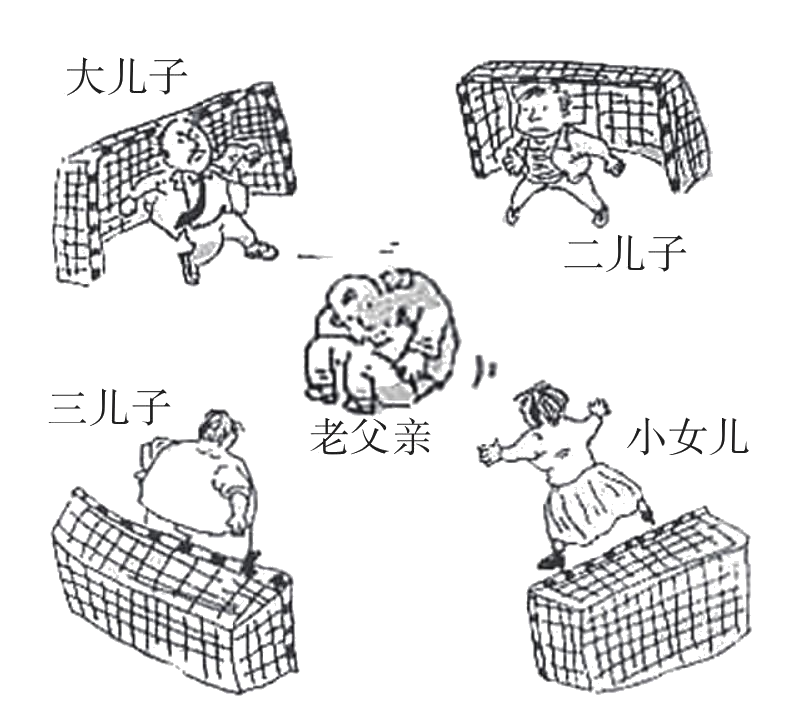
\includegraphics[width=0.56\linewidth]{picture/2005.png}
	\caption*{养老“足球赛”}
\end{figure}


\checkpagenumber







\bta{2006}

\section{Use of English}

\noindent
\textbf{Directions:}\\
Read the following text. Choose the best word (s) for each
	numbered blank and mark A, B, C or D on ANSWER
	SHEET. (10 points)


\TiGanSpace


The homeless make up a growing percentage of America's
population. \cloze , homelessness has reached such proportions
that local governments can't possibly \cloze. To help homeless
people \cloze independence, the federal government must support
job training programs, \cloze the minimum wage, and fund more
low-cost housing.

\cloze everyone agrees on the number of Americans who are
homeless. Estimates \cloze anywhere from 600,000 to 3
million. \cloze the figure may vary, analysts do agree on another
matter: that the number of the homeless is \cloze. One of the
federal government's studies \cloze that the number of the
homeless will reach nearly 19 million by the end of this decade.

Finding ways to \cloze this growing homeless population has
become increasingly difficult. \cloze when homeless individuals
manage to find a \cloze that will give them three meals a day
and a place to sleep at night, a good number still spend the bulk of
each day \cloze the street. Part of the problem is that many
homeless adults are addicted to alcohol or drugs. And a significant
number of the homeless have serious mental disorders. Many
others, \cloze not addicted or mentally ill, simply lack the
everyday \cloze skills needed to turn their
lives \cloze. \emph{Boston Globe} reporter Chris Reidy notes
that the situation will improve only when there
are \cloze programs that address the many needs of the
homeless. \cloze Edward Zlotkowski, director of community
service at Bentley College in Massachusetts, \cloze it, ``There
has to be \cloze of programs. What's needed is a package deal.''


\newpage
\begin{enumerate}
	%\renewcommand{\labelenumi}{\arabic{enumi}.}
	% A(\Alph) a(\alph) I(\Roman) i(\roman) 1(\arabic)
	%设定全局标号series=example	%引用全局变量resume=example
	%[topsep=-0.3em,parsep=-0.3em,itemsep=-0.3em,partopsep=-0.3em]
	%可使用leftmargin调整列表环境左边的空白长度 [leftmargin=0em]
	\item
\fourchoices
{Indeed}
{Likewise}
{Therefore}
{Furthermore}




\item
\fourchoices
{stand}
{cope}
{approve}
{retain}




\item
\fourchoices
{in}
{for}
{with}
{toward}




\item
\fourchoices
{raise}
{add}
{take}
{keep}




\item

\fourchoices
{Generally}
{Almost}
{Hardly}
{Not}




\item

\fourchoices
{cover}
{change}
{range}
{differ}




\item

\fourchoices
{Now that}
{Although}
{Provided}
{Except that}




\item
\fourchoices
{inflating}
{expanding}
{increasing}
{extending}




\item
\fourchoices
{predicts}
{displays}
{proves}
{discovers}




\item
\fourchoices
{assist}
{track}
{sustain}
{dismiss}




\item

\fourchoices
{Hence}
{But}
{Even}
{Only}




\item

\fourchoices
{lodging}
{shelter}
{dwelling}
{house}




\item
\fourchoices
{searching}
{strolling}
{crowding}
{wandering}



\item

\fourchoices
{when}
{once}
{while}
{whereas}




\item

\fourchoices
{life}
{existence}
{survival}
{maintenance}




\item

\fourchoices
{around}
{over}
{on}
{up}




\item
\fourchoices
{complex}
{comprehensive}
{complementary}
{compensating}



\item

\fourchoices
{So}
{Since}
{As}
{Thus}




\item

\fourchoices
{puts}
{interprets}
{assumes}
{makes}




\item
\fourchoices
{supervision}
{manipulation}
{regulation}
{coordination}

\end{enumerate}

\vfil

\section{Reading Comprehension}



\noindent
\textbf{Part A}\\
\textbf{Directions:}\\
Read the following four texts. Answer the questions below each
text by choosing A, B, C, or D  Mark your
answers on ANSWER SHEET. (40 points)



\newpage
\subsection{Text 1}


In spite of  ``endless talk of difference,'' American society is an
amazing machine for homogenizing people. There is ``the democratizing
uniformity of dress and discourse, and the casualness and absence of
deference'' characteristic of popular culture. People are absorbed into
``a culture of consumption'' launched by the 19 th-century department
stores that offered ``vast arrays of goods in an elegant atmosphere.
Instead of intimate shops catering to a knowledgeable elite'' these were
stores ``anyone could enter, regardless of class or background. This
turned shopping into a public and democratic act.'' The mass media,
advertising and sports are other forces for homogenization.

Immigrants are quickly fitting into this common culture, which may not
be altogether elevating but is hardly poisonous. Writing for the
National Immigration Forum, Gregory Rodriguez reports that today's
immigration is neither at unprecedented levels nor resistant to
assimilation. In 1998 immigrants were 9.8 percent of the population; in
1900, 13.6 percent. In the 10 years prior to 1990, 3.1 immigrants
arrived for every 1, 000 residents; in the 10 years prior to 1890, 9.2
for every 1, 000. Now, consider three indices of assimilation---language,
home ownership and intermarriage.

The 1990 Census revealed that ``a majority of immigrants from each of
the fifteen most common countries of origin spoke English `well' or
`very well' after ten years of residence.'' The children of immigrants
tend to be bilingual and proficient in English. ``By the third
generation, the original language is lost in the majority of immigrant
families.'' Hence the description of America as a ``graveyard'' for
languages. By 1996 foreign-born immigrants who had arrived before 1970
had a home ownership rate of 75.6 percent, higher than the 69.8 percent
rate among native-born Americans.

Foreign-born Asians and Hispanics ``have higher rates of intermarriage
than do U.S.-born whites and blacks.'' By the third generation, one
third of Hispanic women are married to non-Hispanics, and 41 percent of
Asian-American women are married to non-Asians.

Rodriguez notes that children in remote villages around the world are
fans of superstars like Arnold Schwarzenegger and Garth Brooks, yet
``some Americans fear that immigrants living within the United States
remain somehow immune to the nation's assimilative power.''

Are there divisive issues and pockets of seething anger in America?
Indeed. It is big enough to have a bit of everything. But particularly
when viewed against America's turbulent past, today's social indices
hardly suggest a dark and deteriorating social environment.



\begin{enumerate}[resume]
	%\renewcommand{\labelenumi}{\arabic{enumi}.}
	% A(\Alph) a(\alph) I(\Roman) i(\roman) 1(\arabic)
	%设定全局标号series=example	%引用全局变量resume=example
	%[topsep=-0.3em,parsep=-0.3em,itemsep=-0.3em,partopsep=-0.3em]
	%可使用leftmargin调整列表环境左边的空白长度 [leftmargin=0em]
	\item
The word ``homogenizing'' (Line 2, Paragraph 1) most
probably means \lineread.

\fourchoices
{identifying}
{associating}
{assimilating}
{monopolizing}



\item
According to the author, the department stores of the 19th
century \lineread.

\fourchoices
{played a role in the spread of popular culture}
{became intimate shops for common consumers}
{satisfied the needs of a knowledgeable elite}
{owed its emergence to the culture of consumption}


\item
The text suggests that immigrants now in the U.S.
\lineread .

\fourchoices
{are resistant to homogenization}
{exert a great influence on American culture}
{are hardly a threat to the common culture}
{constitute the majority of the population}



\item
Why are Arnold Schwarzenegger and Garth Brooks mentioned in
Paragraph 5?

\fourchoices
{To prove their popularity around the world.}
{To reveal the public's fear of immigrants.}
{To give examples of successful immigrants.}
{To show the powerful influence of American culture.}



\item
 In the author's opinion, the absorption of immigrants into
American society is \lineread.

\fourchoices
{rewarding}
{successful}
{fruitless}
{harmful}


\end{enumerate}

\newpage
\subsection{Text 2}


Stratford-on-Avon, as we all know, has only one industry---William
Shakespeare---but there are two distinctly separate and increasingly
hostile branches. There is the Royal Shakespeare Company (RSC), which
presents superb productions of the plays at the Shakespeare Memorial
Theatre on the Avon. And there are the townsfolk who largely live off
the tourists who come, not to see the plays, but to look at Anne
Hathaway's Cottage, Shakespeare's birthplace and the other sights.

The worthy residents of Stratford doubt that the theatre adds a penny
to their revenue. They frankly dislike the RSC's actors, them with their
long hair and beards and sandals and noisiness. It's all deliciously
ironic when you consider that Shakespeare, who earns their living, was
himself an actor (with a beard) and did his share of noise-making.

The tourist streams are not entirely separate. The sightseers who come
by bus---and often take in Warwick Castle and Blenheim Palace on the
side---don't usually see the plays, and some of them are even surprised
to find a theatre in Stratford. However, the playgoers do manage a
little sight-seeing along with their playgoing. It is the playgoers, the
RSC contends, who bring in much of the town's revenue because they spend
the night (some of them four or five nights) pouring cash into the
hotels and restaurants. The sightseers can take in everything and get
out of town by nightfall.

The townsfolk don't see it this way and the local council does not
contribute directly to the subsidy of the Royal Shakespeare Company.
Stratford cries poor traditionally. Nevertheless every hotel in town
seems to be adding a new wing or cocktail lounge. Hilton is building its
own hotel there, which you may be sure will be decorated with Hamlet
Hamburger Bars, the Lear Lounge, the Banquo Banqueting Room, and so
forth, and will be very expensive.

Anyway, the townsfolk can't understand why the Royal Shakespeare Company
needs a subsidy. (The theatre has broken attendance records for three
years in a row. Last year its 1, 431 seats were 94 per cent occupied all
year long and this year they'll do better.) The reason, of course, is
that costs have rocketed and ticket prices have stayed low.

It would be a shame to raise prices too much because it would drive away
the young people who are Stratford's most attractive clientele. They
come entirely for the plays, not the sights. They all seem to look alike
(though they come from all over)---lean, pointed, dedicated faces,
wearing jeans and sandals, eating their buns and bedding down for the
night on the flagstones outside the theatre to buy the 20 seats and 80
standing-room tickets held for the sleepers and sold to them when the
box office opens at 10:30 a.m.


\begin{enumerate}[resume]
	%\renewcommand{\labelenumi}{\arabic{enumi}.}
	% A(\Alph) a(\alph) I(\Roman) i(\roman) 1(\arabic)
	%设定全局标号series=example	%引用全局变量resume=example
	%[topsep=-0.3em,parsep=-0.3em,itemsep=-0.3em,partopsep=-0.3em]
	%可使用leftmargin调整列表环境左边的空白长度 [leftmargin=0em]
	\item
From the first two paragraphs, we learn that \lineread.


\fourchoices
{the townsfolk deny the RSC's contribution to the town's revenue}
{the actors of the RSC imitate Shakespeare on and off stage}
{the two branches of the RSC are not on good terms}
{the townsfolk earn little from tourism}



\item
It can be inferred from Paragraph 3 that \lineread.


\fourchoices
{the sightseers cannot visit the Castle and the Palace separately}
{the playgoers spend more money than the sightseers}
{the sightseers do more shopping than the playgoers}
{the playgoers go to no other places in town than the theater}



\item
By saying ``Stratford cries poor traditionally'' (Line 2,
Paragraph 4), the author implies that \lineread.


\fourchoices
{Stratford cannot afford the expansion projects}
{Stratfordhas long been in financial difficulties}
{the town is not really short of money}
{the townsfolk used to be poorly paid}


\item
 According to the townsfolk, the RSC deserves no subsidy
because \lineread.


\fourchoices
{ticket prices can be raised to cover the spending}
{the company is financially ill-managed}
{the behavior of the actors is not socially acceptable}
{the theatre attendance is on the rise}


\item
From the text we can conclude that the author \lineread.


\fourchoices
{is supportive of both sides}
{favors the townsfolk's view}
{takes a detached attitude}
{is sympathetic to the RSC}



\end{enumerate}


\newpage
\subsection{Text 3}


When prehistoric man arrived in new parts of the world, something
strange happened to the large animals: they suddenly became extinct.
Smaller species survived. The large, slow-growing animals were easy
game, and were quickly hunted to extinction. Now something similar could
be happening in the oceans.

That the seas are being overfished has been known for years. What
researchers such as Ransom Myers and Boris Worm have shown is just how
fast things are changing. They have looked at half a century of data
from fisheries around the world. Their methods do not attempt to
estimate the actual biomass (the amount of living biological matter) of
fish species in particular parts of the ocean, but rather changes in
that biomass over time. According to their latest paper published in
\emph{Nature}, the biomass of large predators (animals that kill and eat
other animals) in a new fishery is reduced on average by 80\% within 15
years of the start of exploitation. In some long-fished areas, it has
halved again since then.

Dr. Worm acknowledges that these figures are conservative. One reason
for this is that fishing technology has improved. Today's vessels can
find their prey using satellites and sonar, which were not available 50
years ago. That means a higher proportion of what is in the sea is being
caught, so the real difference between present and past is likely to be
worse than the one recorded by changes in catch sizes. In the early
days, too, longlines would have been more saturated with fish. Some
individuals would therefore not have been caught, since no baited hooks
would have been available to trap them, leading to an underestimate of
fish stocks in the past. Furthermore, in the early days of longline
fishing, a lot of fish were lost to sharks after they had been hooked.
That is no longer a problem, because there are fewer sharks around now.

Dr. Myers and Dr. Worm argue that their work gives a correct baseline,
which future management efforts must take into account. They believe the
data support an idea current among marine biologists, that of the
``shifting baseline''. The notion is that people have failed to detect
the massive changes which have happened in the ocean because they have
been looking back only a relatively short time into the past. That
matters because theory suggests that the maximum sustainable yield that
can be cropped from a fishery comes when the biomass of a target species
is about 50\% of its original levels. Most fisheries are well below
that, which is a bad way to do business.

\begin{enumerate}[resume]
	%\renewcommand{\labelenumi}{\arabic{enumi}.}
	% A(\Alph) a(\alph) I(\Roman) i(\roman) 1(\arabic)
	%设定全局标号series=example	%引用全局变量resume=example
	%[topsep=-0.3em,parsep=-0.3em,itemsep=-0.3em,partopsep=-0.3em]
	%可使用leftmargin调整列表环境左边的空白长度 [leftmargin=0em]
	\item
The extinction of large prehistoric animals is noted to
suggest that \lineread.


\fourchoices
{large animals were vulnerable to the changing environment}
{small species survived as large animals disappeared}
{large sea animals may face the same threat today}
{slow-growing fish outlive fast-growing ones}


\item
We can infer from Dr. Myers and Dr. Worm's paper that
\lineread.


\fourchoices
{the stock of large predators in some old fisheries has reduced by 90\%}
{there are only half as many fisheries as there were 15 years ago}
{the catch sizes in new fisheries are only 20\% of the original amount}
{the number of large predators dropped faster in new fisheries than in the old}




\item
By saying ``these figures are conservative'' (Line 1,
paragraph 3), Dr. Worm means that \lineread.


\fourchoices
{fishing technology has improved rapidly}
{then catch-sizes are actually smaller than recorded}
{the marine biomass has suffered a greater loss}
{the data collected so far are out of date}



\item
Dr. Myers and other researchers hold that \lineread.


\fourchoices
{people should look for a baseline that can work for a longer time}
{fisheries should keep their yields below 50\% of the biomass}
{the ocean biomass should be restored to its original level}
{people should adjust the fishing baseline to the changing situation}



\item
The author seems to be mainly concerned with most fisheries'
\lineread.


\fourchoices
{management efficiency}
{biomass level}
{catch-size limits}
{technological application}

	
\end{enumerate}





\newpage
\subsection{Text 4}


Many things make people think artists are weird. But the weirdest may be
this: artists' only job is to explore emotions, and yet they choose to
focus on the ones that feel bad.

This wasn't always so. The earliest forms of art, like painting and
music, are those best suited for expressing joy. But somewhere from the
19th century onward, more artists began seeing happiness as meaningless,
phony or, worst of all, boring, as we went from Wordsworth's \emph{daffodils}
to Baudelaire's \emph{flowers of evil}.

You could argue that art became more skeptical of happiness because
modern times have seen so much misery. But it's not as if earlier times
didn't know perpetual war, disaster and the massacre of innocents. The
reason, in fact, may be just the opposite: there is too much damn
happiness in the world today.

After all, what is the one modern form of expression almost completely
dedicated to depicting happiness? Advertising. The rise of anti-happy
art almost exactly tracks the emergence of mass media, and with it, a
commercial culture in which happiness is not just an ideal but an
ideology.

People in earlier eras were surrounded by reminders of misery. They
worked until exhausted, lived with few protections and died young. In
the West, before mass communication and literacy, the most powerful mass
medium was the church, which reminded worshippers that their souls were
in danger and that they would someday be meat for worms. Given all this,
they did not exactly need their art to be a bummer too.

Today the messages the average Westerner is surrounded with are not
religious but commercial, and forever happy. Fast-food eaters, news
anchors, text messengers, all smiling, smiling, smiling. Our magazines
feature beaming celebrities and happy families in perfect homes. And
since these messages have an agenda---to lure us to open our
wallets---they make the very idea of happiness seem unreliable.
``Celebrate!'' commanded the ads for the arthritis drug Celebrex, before
we found out it could increase the risk of heart attacks.

But what we forget---what our economy depends on us forgetting---is that
happiness is more than pleasure without pain. The things that bring the
greatest joy carry the greatest potential for loss and disappointment.
Today, surrounded by promises of easy happiness, we need art to tell us,
as religion once did, \emph{Memento mori}: remember that you will die,
that everything ends, and that happiness comes not in denying this but
in living with it. It's a message even more bitter than a clove
cigarette, yet, somehow, a breath of fresh air.



\begin{enumerate}[resume]
	%\renewcommand{\labelenumi}{\arabic{enumi}.}
	% A(\Alph) a(\alph) I(\Roman) i(\roman) 1(\arabic)
	%设定全局标号series=example	%引用全局变量resume=example
	%[topsep=-0.3em,parsep=-0.3em,itemsep=-0.3em,partopsep=-0.3em]
	%可使用leftmargin调整列表环境左边的空白长度 [leftmargin=0em]
	\item
By citing the examples of poets Wordsworth and Baudelaire,
the author intends to show that \lineread.


\fourchoices
{poetry is not as expressive of joy as painting or music}
{art grows out of both positive and negative feelings}
{poets today are less skeptical of happiness}
{artists have changed their focus of interest}



\item
The word ``bummer'' (Line 5, paragraph 5) most probably
means something \lineread.


\fourchoices
{religious}
{unpleasant}
{entertaining}
{commercial}


\item
In the author's opinion, advertising \lineread.


\fourchoices
{emerges in the wake of the anti-happy art}
{is a cause of disappointment for the general public}
{replace the church as a major source of information}
{creates an illusion of happiness rather than happiness itself}


\item
We can learn from the last paragraph that the author
believes \lineread.


\fourchoices
{happiness more often than not ends in sadness}
{the anti-happy art is distasteful but refreshing}
{misery should be enjoyed rather than denied}
{the anti-happy art flourishes when economy booms}



\item
Which of the following is true of the text?


\fourchoices
{Religion once functioned as a reminder of misery.}
{Art provides a balance between expectation and reality.}
{People feel disappointed at the realities of modern society.}
{Mass media are inclined to cover disasters and deaths.}


\end{enumerate}


\newpage
\noindent
\textbf{Part B}\\
\textbf{Directions:}\\
In the following article, some sentences have been removed. For
Questions 41-45, choose the most suitable one from the list A-G to fit
into each of numbered gaps. There are two extra choices, which you do
not need to use. Mark your answers on ANSWER SHEET. (10 points)



\TiGanSpace


On the north bank of the Ohio River sits Evansville, Ind., home of David
Williams, 52, and of a riverboat casino (a place where gambling games
are played). During several years of gambling in that casino, Williams,
a state auditor earning \$35,000 a year, lost approximately \$175,000.
He had never gambled before the casino sent him a coupon for \$20 worth
of gambling.

He visited the casino, lost the \$20 and left. On his second visit he
lost \$800. The casino issued to him, as a good customer, a ``Fun
Card'', which when used in the casino earns points for meals and drinks,
and enables the casino to track the user's gambling activities. For
Williams, these activities become what he calls ``electronic heroin''.

\linefill. In 1997 he lost \$21,000 to one slot machine in
two days. In March 1997 he lost \$72,186. He sometimes played two slot
machines at a time, all night, until the boat docked at 5 a.m., then
went back aboard when the casino opened at 9 a.m. Now he is suing the
casino, charging that it should have refused his patronage because it
knew he was addicted. It did know he had a problem.

In March 1998 a friend of Williams's got him involuntarily confined to a
treatment center for addictions, and wrote to inform the casino of
Williams's gambling problem. The casino included a photo of Williams
among those of banned gamblers, and wrote to him a ``cease admissions''
letter. Noting the ``medical/psychological'' nature of problem gambling
behavior, the letter said that before being readmitted to the casino he
would have to present medical/psychological information demonstrating
that patronizing the casino would pose no threat to his safety or
well-being.

\linefill.

\emph{The Wall Street Journal} reports that the casino has 24 signs
warning: ``Enjoy the fun... and always bet with your head, not over
it.'' Every entrance ticket lists a toll-free number for counseling from
the Indiana Department of Mental Health. Nevertheless, Williams's suit
charges that the casino, knowing he was ``helplessly addicted to
gambling,'' intentionally worked to ``lure'' him to ``engage in conduct
against his will.''

\linefill.

The fourth edition of \emph{the Diagnostic and Statistical Manual of
	Mental Disorders} says ``pathological gambling'' involves persistent,
recurring and uncontrollable pursuit less of money than of the thrill of
taking risks in quest of a windfall.

\linefill. Pushed by science, or what claims to be science,
society is reclassifying what once were considered character flaws or
moral failings as personality disorders akin to physical disabilities.

\linefill.

Forty-four states have lotteries, 29 have casinos, and most of these
states are to varying degrees dependent on---you might say addicted
to---revenues from wagering. And since the first Internet gambling site
was created in 1995, competition for gamblers' dollars has become
intense. The Oct. 28 issue of \emph{Newsweek} reported that 2 million
gamblers patronize 1,800 virtual casinos every week. With \$3.5
billion being lost on Internet wagers this year, gambling has passed
pornography as the Web's most profitable business.
\begin{listmatch}
	%\renewcommand{\labelenumi}{\arabic{enumi}.}
	% A(\Alph) a(\alph) I(\Roman) i(\roman) 1(\arabic)
	%设定全局标号series=example	%引用全局变量resume=example
	%[topsep=-0.3em,parsep=-0.3em,itemsep=-0.3em,partopsep=-0.3em]
	%可使用leftmargin调整列表环境左边的空白长度 [leftmargin=0em]
	\item
Although no such evidence was presented, the casino's marketing
department continued to pepper him with mailings. And he entered the
casino and used his Fun Card without being detected.


\item 
It is unclear what luring was required, given his compulsive
behavior. And in what sense was his will operative?


\item 
By the time he had lost \$5,000 he said to himself that if he
could get back to even, he would quit. One night he won \$5,500, but he
did not quit.


\item 
 Gambling has been a common feature of American life forever, but
for a long time it was broadly considered a sin, or a social disease.
Now it is a social policy: the most important and aggressive promoter of
gambling in America is the government.


\item 
David Williams's suit should trouble this gambling nation. But
don't bet on it.


\item 
 It is worrisome that society is medicalizing more and more
behavioral problems, often defining as addictions what earlier, sterner
generations explained as weakness of will.


\item 
The anonymous, lonely, undistracted nature of online gambling is
especially conducive to compulsive behavior. But even if the government
knew how to move against Internet gambling, what would be its grounds
for doing so?

\end{listmatch}




\noindent
\textbf{Part C}\\
\textbf{Directions:}\\
Read the following text carefully and then translate the underlined
segments into Chinese. Your translation should be written clearly on
\textbf{ANSWER SHEET}. (10 points)


\TiGanSpace

Is it true that the American intellectual is rejected and considered of
no account in his society? I am going to suggest that it is not true.
Father Bruckberger told part of the story when he observed that it is
the intellectuals who have rejected America. But they have done more
than that. They have grown dissatisfied with the role of the
intellectual. It is they, not America, who have become
anti-intellectual.

First, the object of our study pleads for definition. What is an
intellectual? \transnum \uline{I shall define him as an individual who
	has elected as his primary duty and pleasure in life the activity of
	thinking in a Socratic (苏格拉底) way about moral problems.} He explores
such problems consciously, articulately, and frankly, first by asking
factual questions, then by asking moral questions, finally by suggesting
action which seems appropriate in the light of the factual and moral
information which he has obtained. \transnum \uline{His function is
	analogous to that of a judge, who must accept the obligation of
	revealing in as obvious a matter as possible the course of reasoning
	which led him to his decision.}

This definition excludes many individuals usually referred to as
intellectuals---the average scientist, for one. \transnum \uline{I have
	excluded him because, while his accomplish\-ments may contribute to the
	solution of moral problems, he has not been charged with the task of
	approaching any but the factual aspects of those problems.} Like other
human beings, he encounters moral issues even in the everyday
performance of his routine duties---he is not supposed to cook his
experiments, manufacture evidence, or doctor his reports.
\transnum \uline{But his primary task is not to think about the moral
	code which governs his activity, any more than a businessman is expected
	to dedicate his energies to an exploration of rules of conduct in
	business.} During most of his waking life he will take his code for
granted, as the businessman takes his ethics.

The definition also excludes the majority of teachers, despite the fact
that teaching has traditionally been the method whereby many
intellectuals earn their living. \transnum \uline{They may teach very
	well, and more than earn their salaries, but most of them make little or
	no independent reflections on human problems which involve moral
	judgment.} This description even fits the majority of eminent scholars.
Being learned in some branch of human knowledge is one thing; living in
``public and illustrious thoughts,'' as Emerson would say, is something
else.



\newpage
\section{Writing}


\noindent
\textbf{Part A}\\
\textbf{51. Directions:}

You want to contribute to Project Hope by offering financial aid to a
child in a remote area. Write a letter to the department concerned,
asking them to help find a candidate. You should specify what kind of
child you want to help and how you will carry out your plan.

Write your letter with no less than 100 words. Write it neatly on ANSWER
SHEET.
\textbf{Do not} sign your name at the end of the letter; use ``Li Ming''
instead.
\textbf{Do not} write the address. (10 points)


\vspace{2em}

\noindent
\textbf{Part B}\\
\textbf{52. Directions:}

Study the following photos carefully and write an essay in which you
should
\begin{listwrite}
	\item 
 describe the photos briefly,
\item
interpret the social phenomenon reflected by them, and
\item
give your point of view.
\end{listwrite}

You should write 160-200 words neatly on ANSWER SHEET. (20 points)




\begin{figure}[ht]
	\begin{subfigure}[b]{0.45\linewidth}
		\centering
		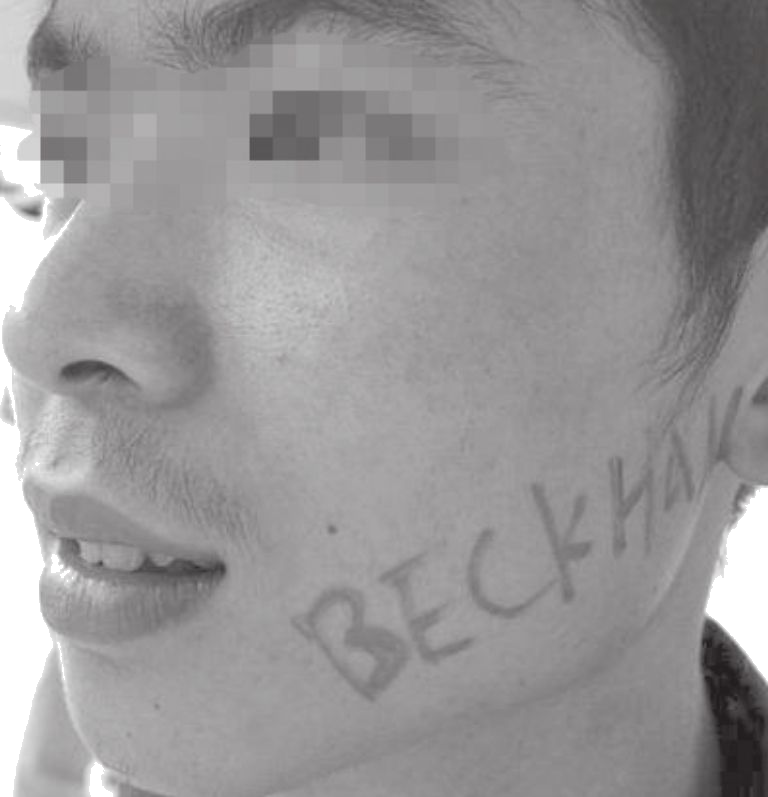
\includegraphics[height=3.5cm]{picture/2006_1.png}
		\caption*{把崇拜写在脸上}
	\end{subfigure}
\hfil
	\begin{subfigure}[b]{0.45\linewidth}
		\centering
		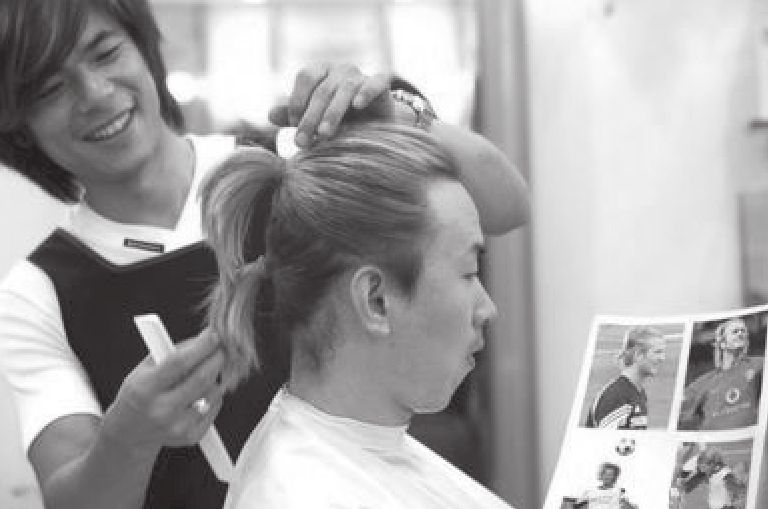
\includegraphics[height=3.5cm]{picture/2006_2.png} 
		\caption*{花300元做个“⼩贝头”}
		\label{fig:2}
	\end{subfigure}
\end{figure}


注:Beckham(贝克汉姆)——英国⾜球明星




%
\bta{2007}






\section{Use of English}

\noindent
\textbf{Directions:}\\
Read the following text. Choose the best word (s) for each numbered blank and mark A, B, C or D on ANSWER SHEET 1. (10 points)



\TiGanSpace


By 1830 the former Spanish and Portuguese colonies had become
independent nations. The roughly 20 million \cloze of these
nations looked \cloze to the future. Born in the crisis of the
old regime and Iberian colonialism, many of the leaders of
independence \cloze the ideals of representative government,
careers \cloze to talent, freedom of commerce and trade,
the \cloze to private property, and a belief in the individual as
the basis of society. \cloze there was a belief that the new
nations should be sovereign and independent states, large enough to be
economically viable and integrated by a \cloze set of laws.

On the issue of \cloze of religion and the position of the
Church, \cloze , there was less agreement \cloze the
leadership. Roman Catholicism had been the state religion and the only
one \cloze by the Spanish crown. \cloze most leaders
sought to maintain Catholicism \cloze the official religion of
the new states, some sought to end the \cloze of other faiths.
The defense of the Church became a rallying \cloze for the
conservative forces.

The ideals of the early leaders of independence were often egalitarian,
valuing equality of everything. Bolivar had received aid from Haiti and
had \cloze in return to abolish slavery in the areas he
liberated. By 1854 slavery had been abolished everywhere except
Spain's \cloze colonies. Early promises to end Indian tribute
and taxes on people of mixed origin came much \cloze because the
new nations still needed the revenue such policies \cloze.
Egalitarian sentiments were often tempered by fears that the mass of the
population was \cloze self-rule and democracy.


\newpage

\begin{enumerate}
	%\renewcommand{\labelenumi}{\arabic{enumi}.}
	% A(\Alph) a(\alph) I(\Roman) i(\roman) 1(\arabic)
	%设定全局标号series=example	%引用全局变量resume=example
	%[topsep=-0.3em,parsep=-0.3em,itemsep=-0.3em,partopsep=-0.3em]
	%可使用leftmargin调整列表环境左边的空白长度 [leftmargin=0em]
	\item
\fourchoices
{natives}
{inhabitants}
{peoples}
{individuals}




\item

\fourchoices
{confusedly}
{cheerfully}
{worriedly}
{hopefully}



\item


\fourchoices
{shared}
{forgot}
{attained}
{rejected}




\item


\fourchoices
{related}
{close}
{open}
{devoted}




\item


\fourchoices
{access}
{succession}
{right}
{return}




\item

\fourchoices
{Presumably}
{Incidentally}
{Obviously}
{Generally}


\item


\fourchoices
{unique}
{common}
{particular}
{typical}




\item


\fourchoices
{freedom}
{origin}
{impact}
{reform}




\item


\fourchoices
{therefore}
{however}
{indeed}
{moreover}




\item


\fourchoices
{with}
{about}
{among}
{by}




\item


\fourchoices
{allowed}
{preached}
{granted}
{funded}




\item


\fourchoices
{Since}
{If}
{Unless}
{While}




\item


\fourchoices
{as}
{for}
{under}
{against}




\item

\fourchoices
{spread}
{interference}
{exclusion}
{influence}




\item


\fourchoices
{support}
{cry}
{plea}
{wish}




\item


\fourchoices
{urged}
{intended}
{expected}
{promised}




\item


\fourchoices
{controlling}
{former}
{remaining}
{original}




\item


\fourchoices
{slower}
{faster}
{easier}
{tougher}




\item

\fourchoices
{created}
{produced}
{contributed}
{preferred}



\item

\fourchoices
{puzzled by}
{hostile to}
{pessimistic about}
{unprepared for}

\end{enumerate}

\vfil

\section{Reading Comprehension}


\noindent
\textbf{Part A}\\
\textbf{Directions:}\\
Read the following four texts. Answer the questions below each
text by choosing A, B, C, or D. . Mark your answers on ANSWER SHEET 1. (40 points)

\newpage
\subsection{Text 1}


If you were to examine the birth certificates of every soccer player in
2006's World Cup tournament, you would most likely find a noteworthy
quirk: elite soccer players are more likely to have been born in the
earlier months of the year than in the late months. If you then examined
the European national youth teams that feed the World Cup and
professional ranks, you would find this strange phenomenon to be ever
more pronounced.

What might account for this strange phenomenon? Here are a few guesses:
a) certain astrological signs confer superior soccer skills; b)
winter-born babies tend to have higher oxygen capacity, which increases
soccer stamina; c) soccer-mad parents are more likely to conceive
children in springtime, at the annual peak of soccer \uline{mania};
d) none of the above.

Anders Ericsson, a 58-year-old psychology professor at Florida State
University, says he believes strongly in ``none of the above.'' Ericsson
grew up in Sweden, and studied nuclear engineering until he realized he
would have more opportunity to conduct his own research if he switched
to psychology. His first experiment, nearly 30 years ago, involved
memory: training a person to hear and then repeat a random series of
numbers. ``With the first subject, after about 20 hours of training, his
digit span had risen from 7 to 20,'' Ericsson recalls. ``He kept
improving, and after about 200 hours of training he had risen to over 80
numbers.''

This success, coupled with later research showing that memory itself is
not genetically determined, led Ericsson to conclude that the act of
memorizing is more of a cognitive exercise than an intuitive one. In
other words, whatever inborn differences two people may exhibit in their
abilities to memorize, those differences are swamped by how well each
person ``encodes'' the information. And the best way to learn how to
encode information meaningfully, Ericsson determined, was a process
known as deliberate practice. Deliberate practice entails more than
simply repeating a task. Rather, it involves setting specific goals,
obtaining immediate feedback and concentrating as much on technique as
on outcome.

Ericsson and his colleagues have thus taken to studying expert
performers in a wide range of pursuits, including soccer. They gather
all the data they can, not just performance statistics and biographical
details but also the results of their own laboratory experiments with
high achievers. Their work makes a rather startling assertion: the trait
we commonly call talent is highly overrated. Or, put another way, expert
performers---whether in memory or surgery, ballet or computer
programming---are nearly always made, not born.


\begin{enumerate}[resume]
	%\renewcommand{\labelenumi}{\arabic{enumi}.}
	% A(\Alph) a(\alph) I(\Roman) i(\roman) 1(\arabic)
	%设定全局标号series=example	%引用全局变量resume=example
	%[topsep=-0.3em,parsep=-0.3em,itemsep=-0.3em,partopsep=-0.3em]
	%可使用leftmargin调整列表环境左边的空白长度 [leftmargin=0em]
	\item
 The birthday phenomenon found among soccer players is
mentioned to \lineread.


\fourchoices
{stress the importance of professional training.}
{spotlight the soccer superstars at the World Cup.}
{introduce the topic of what makes expert performance.}
{explain why some soccer teams play better than others.}


\item
The word ``mania'' (Line 4, Paragraph 2) most probably
means \lineread.



\fourchoices
{fun}
{craze}
{hysteria}
{excitement}




\item
According to Ericsson, good memory \lineread.


\fourchoices
{depends on meaningful processing of information}
{results from intuitive rather than cognitive exercises}
{is determined by genetic rather than psychological factors}
{requires immediate feedback and a high degree of concentration}



\item
Ericsson and his colleagues believe that \lineread.


\fourchoices
{talent is a dominating factor for professional success}
{biographical data provide the key to excellent performance}
{the role of talent tends to be overlooked}
{high achievers owe their success mostly to nurture}



\item
Which of the following proverbs is closest to the message
the text tries to convey?


\fourchoices
{``Faith will move mountains.''}
{``One reaps what one sows.''}
{``Practice makes perfect.''}
{``Like father, like son.''}


\end{enumerate}



\newpage
\subsection{Text 2}


For the past several years, the Sunday newspaper
supplement \emph{Parade} has featured a column called ``Ask Marilyn.''
People are invited to query Marilyn vos Savant, who at age 10 had tested
at a mental level of someone about 23 years old; that gave her an IQ of
228---the highest score ever recorded. IQ tests ask you to complete
verbal and visual analogies, to envision paper after it has been folded
and cut, and to deduce numerical sequences, among other similar tasks.
So it is a bit confusing when vos Savant fields such queries from the
average Joe (whose IQ is 100) as, What's the difference between love and
fondness? Or what is the nature of luck and coincidence? It's not
obvious how the capacity to visualize objects and to figure out
numerical patterns suits one to answer questions that have eluded some
of the best poets and philosophers.

Clearly, intelligence encompasses more than a score on a test. Just what
does it mean to be smart? How much of intelligence can be specified, and
how much can we learn about it from neurology, genetics, computer
science and other fields?

The defining term of intelligence in humans still seems to be the IQ
score, even though IQ tests are not given as often as they used to be.
The test comes primarily in two forms: the Stanford-Binet Intelligence
Scale and the Wechsler Intelligence Scales (both come in adult and
children's version). Generally costing several hundred dollars, they are
usually given only by psychologists, although variations of them
populate bookstores and the World Wide Web. Superhigh scores like vos
Savant's are no longer possible, because scoring is now based on a
statistical population distribution among age peers, rather than simply
dividing the mental age by the chronological age and multiplying by 100.
Other standardized tests, such as the Scholastic Assessment Test (SAT)
and the Graduate Record Exam (GRE), capture the main aspects of IQ
tests.

Such standardized tests may not assess all the important elements
necessary to succeed in school and in life, argues Robert J. Sternberg.
In his article ``How Intelligent Is Intelligence Testing?'', Sternberg
notes that traditional tests best assess analytical and verbal skills
but fail to measure creativity and practical knowledge, components also
critical to problem solving and life success. Moreover, IQ tests do not
necessarily predict so well once populations or situations change.
Research has found that IQ predicted leadership skills when the tests
were given under low-stress conditions, but under high-stress
conditions, IQ was negatively correlated with leadership---that is, it
predicted the opposite. Anyone who has toiled through SAT will testify
that test-taking skill also matters, whether it's knowing when to guess
or what questions to skip.

\begin{enumerate}[resume]
	%\renewcommand{\labelenumi}{\arabic{enumi}.}
	% A(\Alph) a(\alph) I(\Roman) i(\roman) 1(\arabic)
	%设定全局标号series=example	%引用全局变量resume=example
	%[topsep=-0.3em,parsep=-0.3em,itemsep=-0.3em,partopsep=-0.3em]
	%可使用leftmargin调整列表环境左边的空白长度 [leftmargin=0em]
	\item
Which of the following may be required in an intelligence
test?


\fourchoices
{Answering philosophical questions.}
{Folding or cutting paper into different shapes.}
{Telling the differences between certain concepts.}
{Choosing words or graphs similar to the given ones.}



\item
What can be inferred about intelligence testing from
Paragraph 3?


\fourchoices
{People no longer use IQ scores as an indicator of intelligence.}
{More versions of IQ tests are now available on the Internet.}
{The test contents and formats for adults and children may be different.}
{Scientists have defined the important elements of human intelligence.}



\item
People nowadays can no longer achieve IQ scores as high as
vos Savant's because  \lineread.


\fourchoices
{the scores are obtained through different computational procedures}
{creativity rather than analytical skills is emphasized now}
{vos Savant's case is an extreme one that will not repeat}
{the defining characteristic of IQ tests has changed}



\item
We can conclude from the last paragraph that \lineread.


\fourchoices
{test scores may not be reliable indicators of one's ability}
{IQ scores and SAT results are highly correlated}
{testing involves a lot of guesswork}
{traditional tests are out of date}


\item
What is the author's attitude towards IQ tests?


\fourchoices
{Supportive.}
{Skeptical.}
{Impartial.}
{Biased.}


\end{enumerate}



\newpage
\subsection{Text 3}


During the past generation, the American middle-class family that once
could count on hard work and fair play to keep itself financially secure
has been transformed by economic risk and new realities. Now a pink slip,
a bad diagnosis, or a disappearing spouse can reduce a family from
solidly middle class to newly poor in a few months.

In just one generation, millions of mothers have gone to
work, transforming basic family economics. Scholars, policymakers, and
critics of all stripes have debated the social implications of these
changes, but few have looked at the side effect: family risk has risen
as well. Today's families have budgeted to the limits of theirs new
two-paycheck status. As a result, they have lost the parachute they once
had in times of financial setback---a back-up earner (usually Mom) who
could go into the workforce if the primary earner got laid off or fell
sick. This ``added-worker effect'' could support the safety net offered
by unemployment insurance or disability insurance to help families
weather bad times. But today, a disruption to family fortunes can no
longer be made up with extra income from an otherwise-stay-at-home
partner.

During the same period, families have been asked to absorb much more
risk in their retirement income. Steelworkers, airline employees, and
now those in the auto industry are joining millions of families who must
worry about interest rates, stock market fluctuation, and the harsh
reality that they may outlive their retirement money. For much of the
past year, President Bush campaigned to move Social Security to a
savings-account model, with retirees trading much or all of their
guaranteed payments for payments depending on investment returns. For
younger families, the picture is not any better. Both the absolute cost
of healthcare and the share of it borne by families have risen---and
newly fashionable health-savings plans are spreading from legislative
halls to Wal-Mart workers, with much higher deductibles and a large new
dose of investment risk for families' future healthcare. Even
demographics are working against the middle class family, as the odds of
having a weak elderly parent---and all the attendant need for physical
and financial assistance---have jumped eightfold in just one generation.

From the middle-class family perspective, much of this, understandably,
looks far less like an opportunity to exercise more financial
responsibility, and a good deal more like a frightening acceleration of
the wholesale shift of financial risk onto their already overburdened
shoulders. The financial fallout has begun, and the political fallout
may not be far behind.

\begin{enumerate}[resume]
	%\renewcommand{\labelenumi}{\arabic{enumi}.}
	% A(\Alph) a(\alph) I(\Roman) i(\roman) 1(\arabic)
	%设定全局标号series=example	%引用全局变量resume=example
	%[topsep=-0.3em,parsep=-0.3em,itemsep=-0.3em,partopsep=-0.3em]
	%可使用leftmargin调整列表环境左边的空白长度 [leftmargin=0em]
	\item
Today's double-income families are at greater financial risk
in that \lineread.


\fourchoices
{the safety net they used to enjoy has disappeared}
{their chances of being laid off have greatly increased}
{they are more vulnerable to changes in family economics}
{they are deprived of unemployment or disability insurance}



\item
As a result of President Bush's reform, retired people may
have \lineread.


\fourchoices
{a higher sense of security}
{less secured payments}
{less chance to invest}
{a guaranteed future}




\item
According to the author, health-savings plans will \lineread.


\fourchoices
{help reduce the cost of healthcare}
{popularize among the middle class}
{compensate for the reduced pensions}
{increase the families' investment risk}



\item
 It can be inferred from the last paragraph that \lineread.


\fourchoices
{financial risks tend to outweigh political risks}
{the middle class may face greater political challenges}
{financial problems may bring about political problems}
{financial responsibility is an indicator of political status}


\item
Which of the following is the best title for this text?


\fourchoices
{The Middle Class on the Alert}
{The Middle Class on the Cliff}
{The Middle Class in Conflict}
{The Middle Class in Ruins}


\end{enumerate}


\newpage
\subsection{Text 4}


\uline{It never rains but it pours}. Just as bosses and boards have finally
sorted out their worst accounting and compliance troubles, and improved
their feeble corporation governance, a new problem threatens to earn
them---especially in America---the sort of nasty headlines that
inevitably lead to heads rolling in the executive suite: data
insecurity. Left, until now, to odd, low-level IT staff to put right,
and seen as a concern only of data-rich industries such as banking,
telecoms and air travel, information protection is now high on the
boss's agenda in businesses of every variety.

Several massive leakages of customer and employee data this year---from
organizations as diverse as Time Warner, the American defense contractor
Science Applications International Corp and even the University of
California, Berkeley---have left managers hurriedly peering into their
intricate IT systems and business processes in search of potential
vulnerabilities.

``Data is becoming an asset which needs to be guarded as much as any
other asset,'' says Haim Mendelson of Stanford University's business
school. ``The ability to guard customer data is the key to market value,
which the board is responsible for on behalf of shareholders.'' Indeed,
just as there is the concept of Generally Accepted Accounting Principles
(GAAP), perhaps it is time for GASP, Generally Accepted Security
Practices, suggested Eli Noam of New York's Columbia Business School.
``Setting the proper investment level for security, redundancy, and
recovery is a management issue, not a technical one,'' he says.

The mystery is that this should come as a surprise to any boss. Surely
it should be obvious to the dimmest executive that trust, that most
valuable of economic assets, is easily destroyed and hugely expensive to
restore---and that few things are more likely to destroy trust than a
company letting sensitive personal data get into the wrong hands.

The current state of affairs may have been encouraged---though not
justified---by the lack of legal penalty (in America, but not Europe)
for data leakage. Until California recently passed a law, American firms
did not have to tell anyone, even the victim, when data went astray.
That may change fast: lots of proposed data-security legislation is now
doing the rounds in Washington,
D.C. Meanwhile, the theft of information
about some 40 million credit-card accounts in America, disclosed on June
17th, overshadowed a hugely important decision a day
earlier by America's Federal Trade Commission (FTC) that puts corporate
America on notice that regulators will act if firms fail to provide
adequate data security.

\begin{enumerate}[resume]
	%\renewcommand{\labelenumi}{\arabic{enumi}.}
	% A(\Alph) a(\alph) I(\Roman) i(\roman) 1(\arabic)
	%设定全局标号series=example	%引用全局变量resume=example
	%[topsep=-0.3em,parsep=-0.3em,itemsep=-0.3em,partopsep=-0.3em]
	%可使用leftmargin调整列表环境左边的空白长度 [leftmargin=0em]
	\item
The statement ``It never rains but it pours'' is used to
introduce \lineread.


\fourchoices
{the fierce business competition}
{the feeble boss-board relations}
{the threat from news reports}
{the severity of data leakage.}



\item
 According to Paragraph 2, some organizations check their
systems to find out \lineread.


\fourchoices
{whether there is any weak point}
{what sort of data has been stolen}
{who is responsible for the leakage}
{how the potential spies can be located}



\item
In bringing up the concept of GASP the author is making the
point that \lineread.


\fourchoices
{shareholders' interests should be properly attended to}
{information protection should be given due attention}
{businesses should enhance their level of accounting security}
{the market value of customer data should be emphasized}



\item
 According to Paragraph 4, what puzzles the author is that
some bosses fail to \lineread.


\fourchoices
{see the link between trust and data protection}
{perceive the sensitivity of personal data}
{realize the high cost of data restoration}
{appreciate the economic value of trust}



\item
It can be inferred from Paragraph 5 that \lineread.


\fourchoices
{data leakage is more severe in Europe}
{FTC's decision is essential to data security}
{California takes the lead in security legislation}
{legal penalty is a major solution to data leakage}


\end{enumerate}



\newpage

\noindent
\textbf{Part B}\\
\textbf{Directions:}\\
You are going to read a list of headings and a text about what
parents are supposed to do to guide their children into adulthood.
Choose a heading from the list A-G that best fits the meaning of each
numbered part of the text (41-45). The first and last paragraphs of the
text are not numbered. There are two extra headings that you do not need
to use. Mark your answers on ANSWER SHEET 1. (10 points)


\TiGanSpace


\begin{listmatch}
\item 
Set a Good Example for Your Kids


\item 
Build Your Kids' Work Skills


\item 
Place Time Limits on Leisure Activities


\item 
Talk about the Future on a Regular Basis


\item 
Help Kids Develop Coping Strategies


\item 
Help Your Kids Figure Out Who They Are


\item 
 Build Your Kids' Sense of Responsibility
\end{listmatch}



\begin{center}
\textbf{How Can a Parent Help?}
\end{center}


Mothers and fathers can do a lot to ensure a safe landing in early
adulthood for their kids. Even if a job's starting salary seems too
small to satisfy an emerging adult's need for rapid content, the
transition from school to work can be less of a setback if the start-up
adult is ready for the move. Here are a few measures, drawn from my
book \emph{Ready or Not, Here Life Comes}, that parents can take to
prevent what I call ``work-life unreadiness'':


 \begin{tabular}{|c|c|}
 \hline 
41.  &   \hspace{10em}  \\ 
 \hline 
 \end{tabular}



You can start this process when they are 11 or 12. Periodically review
their emerging strengths and weaknesses with them and work together on
any shortcomings, like difficulty in communicating well or
collaborating. Also, identify the kinds of interests they keep coming
back to, as these offer clues to the careers that will fit them best.

 \begin{tabular}{|c|c|}
	\hline 
	42.  &   \hspace{10em}  \\ 
	\hline 
\end{tabular}

Kids need a range of authentic role models---as opposed to members of
their clique, pop stars and vaunted athletes. Have regular dinner-table
discussions about people the family knows and how they got where they
are. Discuss the joys and downsides of your own career and encourage
your kids to form some ideas about their own future. When asked what
they want to do, they should be discouraged from saying ``I have no
idea.'' They can change their minds 200 times, but having only a foggy
view of the future is of little good.

 \begin{tabular}{|c|c|}
	\hline 
	43.  &   \hspace{10em}  \\ 
	\hline 
\end{tabular}

Teachers are responsible for teaching kids how to learn; parents should
be responsible for teaching them how to work. Assign responsibilities
around the house and make sure homework deadlines are met. Encourage
teenagers to take a part-time job. Kids need plenty of practice delaying
gratification and deploying effective organizational skills, such as
managing time and setting priorities.

 \begin{tabular}{|c|c|}
	\hline 
	44.  &   \hspace{10em}  \\ 
	\hline 
\end{tabular}

Playing video games encourages immediate content. And hours of watching
TV shows with canned laughter only teaches kids to process information
in a passive way. At the same time, listening through earphones to the
same monotonous beats for long stretches encourages kids to stay inside
their bubble instead of pursuing other endeavors. All these activities
can prevent the growth of important communication and thinking skills
and make it difficult for kids to develop the kind of sustained
concentration they will need for most jobs.



 \begin{tabular}{|c|c|}
	\hline 
	45.  &   \hspace{10em}  \\ 
	\hline 
\end{tabular}


They should know how to deal with setbacks, stress and feelings of
inadequacy. They should also learn how to solve problems and resolve
conflicts, ways to brainstorm and think critically. Discussions at home
can help kids practice doing these things and help them apply these
skills to everyday life situations.

What about the son or daughter who is grown but seems to be struggling
and wandering aimlessly through early adulthood? Parents still have a
major role to play, but now it is more delicate. They have to be careful
not to come across as disappointed in their child. They should exhibit
strong interest and respect for whatever currently interests their
fledging adult (as naive or ill conceived as it may seem) while becoming
a partner in exploring options for the future. Most of all, these new
adults must feel that they are respected and supported by a family that
appreciates them.

%刷新计数器
\phantom{\linefill.\linefill.\linefill.\linefill.\linefill.}



\noindent
\textbf{Part C}\\
\textbf{Directions:}\\
Read the following text carefully and then translate the
underlined segments into Chinese. Your translation should be written
neatly on \textbf{ANSWER SHEET 2}. (10 points)


The study of law has been recognized for centuries as a basic
intellectual discipline in European universities. However, only in
recent years has it become a feature of undergraduate programs in
Canadian universities. \transnum \uline{Traditionally, legal learning has
been viewed in such institutions as the special preserve of lawyers,
rather than a necessary part of the intellectual equipment of an
educated person.} Happily, the older and more continental view of legal
education is establishing itself in a number of Canadian universities
and some have even begun to offer undergraduate degrees in law.

If the study of law is beginning to establish itself as part and parcel
of a general education, its aims and methods should appeal directly to
journalism educators. Law is a discipline which encourages responsible
judgment. On the one hand, it provides opportunities to analyze such
ideas as justice, democracy and freedom. \transnum \uline{On the other,
it links these concepts to everyday realities in a manner which is
parallel to the links journalists forge on a daily basis as they cover
and comment on the news.} For example, notions of evidence and fact, of
basic rights and public interest are at work in the process of
journalistic judgment and production just as in courts of law.
Sharpening judgment by absorbing and reflecting on law is a desirable
component of a journalist's intellectual preparation for his or her
career.

\transnum \uline{But the idea that the journalist must understand the law
more profoundly than an ordinary citizen rests on an understanding of
the established conventions and special responsibilities of the news
media.} Politics or, more broadly, the functioning of the state, is a
major subject for journalists. The better informed they are about the
way the state works, the better their reporting will be.
\transnum \uline{In fact, it is difficult to see how journalists who do
not have a clear grasp of the basic features of the Canadian
Constitution can do a competent job on political stories.}

Furthermore, the legal system and the events which occur within it are
primary subjects for journalists. While the quality of legal journalism
varies greatly, there is an undue reliance amongst many journalists on
interpretations supplied to them by lawyers. \transnum \uline{While
comment and reaction from lawyers may enhance stories, it is preferable
for journalists to rely on their own notions of significance and make
their own judgments.} These can only come from a well-grounded
understanding of the legal system.




\newpage

\section{Writing}


\noindent
\textbf{Part A}\\
\textbf{51. Directions:}

Write a letter to your university library, making suggestions for
improving its service.

You should write about 100 words on ANSWER SHEET 2.

\textbf{Do not} sign your own name at the end of the letter. Use ``Li
Ming'' instead.

\textbf{Do not} write the address. (10 points)


\vspace{2em}


\noindent
\textbf{Part B}\\
\textbf{52. Directions:}

Write an essay of 160-200 words based on the following drawing. In your
essay, you should
\begin{listwrite}
	\item
 describe the drawing briefly,

\item 
 explain its intended meaning, and then

\item 
 support your view with an example/examples.
\end{listwrite}

You should write neatly on ANSWER SHEET 2. (20 points)

\begin{figure}[h!]
	\centering
	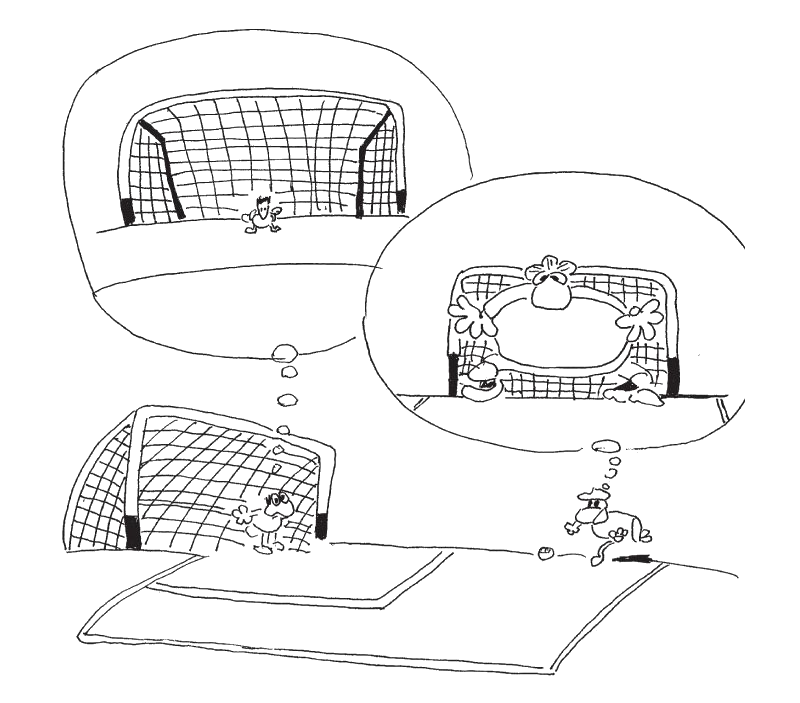
\includegraphics[width=0.56\linewidth]{picture/2007.png}
\end{figure}

\checkpagenumber%




\bta{2008}




\section{Use of English}

\noindent
\textbf{Directions:}\\
Read the following text. Choose the best word (s) for each
	numbered blank and mark A, B, C or D on ANSWER
	SHEET 1. (10 points)
	
	
\TiGanSpace	
	

The idea that some groups of people may be more intelligent than others
is one of those hypotheses that dare not speak its name. But Gregory
Cochran is \cloze to say it anyway. He is
that \cloze bird, a scientist who works
independently \cloze any institution. He helped popularize the
idea that some diseases not \cloze thought to have a bacterial
cause were actually infections, which aroused much controversy when it
was first suggested.

\cloze he, however, might tremble at the \cloze of what he
is about to do. Together with another two scientists, he is publishing a
paper which not only \cloze that one group of humanity is more
intelligent than the others, but explains the process that has brought
this about. The group in \cloze are a particular people originated
from central Europe. The process is natural selection.

This group generally do well in IQ test, \cloze 12-15 points
above the \cloze value of 100, and have
contributed \cloze to the intellectual and cultural life of the
West, as the \cloze of their elites, including several
world-renowned scientists, \cloze. They also suffer more often
than most people from a number of nasty genetic diseases, such as breast
cancer. These facts, \cloze , have previously been thought
unrelated. The former has been \cloze to social effects, such as
a strong tradition of \cloze education. The latter was seen as a(an) \cloze of genetic isolation. Dr. Cochran suggests that the
intelligence and diseases are intimately \cloze. His argument
is that the unusual history of these people has \cloze them to
unique evolutionary pressures that have resulted in
this \cloze state of affairs.



\newpage

\begin{enumerate}
	%\renewcommand{\labelenumi}{\arabic{enumi}.}
	% A(\Alph) a(\alph) I(\Roman) i(\roman) 1(\arabic)
	%设定全局标号series=example	%引用全局变量resume=example
	%[topsep=-0.3em,parsep=-0.3em,itemsep=-0.3em,partopsep=-0.3em]
	%可使用leftmargin调整列表环境左边的空白长度 [leftmargin=0em]
	\item


\fourchoices
{selected}
{prepared}
{obliged}
{pleased}




\item


\fourchoices
{unique}
{particular}
{special}
{rare}




\item


\fourchoices
{of}
{with}
{in}
{against}




\item

\fourchoices
{subsequently}
{presently}
{previously}
{lately}




\item


\fourchoices
{Only}
{So}
{Even}
{Hence}




\item


\fourchoices
{thought}
{sight}
{cost}
{risk}




\item


\fourchoices
{advises}
{suggests}
{protests}
{objects}




\item


\fourchoices
{progress}
{fact}
{need}
{question}




\item


\fourchoices
{attaining}
{scoring}
{reaching}
{calculating}




\item


\fourchoices
{normal}
{common}
{mean}
{total}




\item

\fourchoices
{unconsciously}
{disproportionately}
{indefinitely}
{unaccountably}




\item


\fourchoices
{missions}
{fortunes}
{interests}
{careers}




\item


\fourchoices
{affirm}
{witness}
{observe}
{approve}




\item


\fourchoices
{moreover}
{therefore}
{however}
{meanwhile}




\item


\fourchoices
{given up}
{got over}
{carried on}
{put down}




\item

\fourchoices
{assessing}
{supervising}
{administering}
{valuing}




\item

\fourchoices
{development}
{origin}
{consequence}
{instrument}



\item


\fourchoices
{linked}
{integrated}
{woven}
{combined}




\item


\fourchoices
{limited}
{subjected}
{converted}
{directed}




\item

\fourchoices
{paradoxical}
{incompatible}
{inevitable}
{continuous}


	
\end{enumerate}


\vfil

\section{Reading Comprehension}




\noindent
\textbf{Part A}\\
\textbf{Directions:}\\
Read the following four texts. Answer the questions below each
text by choosing A, B, C or
D. Mark your answers
on ANSWER SHEET 1. (40 points)


\newpage
\subsection{Text 1}


While still catching up to men in some spheres of modern life, women
appear to be way ahead in at least one undesirable category. ``Women are
particularly susceptible to developing depression and anxiety disorders
in response to stress compared to men,'' according to Dr. Yehuda, chief
psychiatrist at New York's Veteran's Administration Hospital.

Studies of both animals and humans have shown that sex hormones somehow
affect the stress response, causing females under stress to produce more
of the trigger chemicals than do males under the same conditions. In
several of the studies, when stressed-out female rats had their ovaries
(the female reproductive organs) removed, their chemical responses
became equal to those of the males.

Adding to a woman's increased dose of stress chemicals, are her
increased ``opportunities'' for stress. ``It's not necessarily that
women don't cope as well. It's just that they have so much more to cope
with,'' says Dr. Yehuda. ``Their capacity for tolerating stress may even
be greater than men's,'' she observes, ``it's just that they're dealing
with so many more things that they become worn out from it more visibly
and sooner.''

Dr. Yehuda notes another difference between the sexes. ``I think that
the kinds of things that women are exposed to tend to be in more of a
chronic or repeated nature. Men go to war and are exposed to combat
stress. Men are exposed to more acts of random physical violence. The
kinds of interpersonal violence that women are exposed to tend to be in
domestic situations, by, unfortunately, parents or other family members,
and they tend not to be one-shot deals. The wear-and-tear that comes
from these longer relationships can be quite devastating.''

Adeline Alvarez married at 18 and gave birth to a son, but was
determined to finish college. ``I struggled a lot to get the college
degree. I was living in so much frustration that that was my escape, to
go to school, and get ahead and do better.'' Later, her marriage ended
and she became a single mother. ``It's the hardest thing to take care of
a teenager, have a job, pay the rent, pay the car payment, and pay the
debt. \uline{I lived from paycheck to paycheck}.''

Not everyone experiences the kinds of severe chronic stresses Alvarez
describes. But most women today are coping with a lot of obligations,
with few breaks, and feeling the strain. Alvarez's experience
demonstrates the importance of finding ways to diffuse stress before it
threatens your health and your ability to function.


\begin{enumerate}[resume]
	%\renewcommand{\labelenumi}{\arabic{enumi}.}
	% A(\Alph) a(\alph) I(\Roman) i(\roman) 1(\arabic)
	%设定全局标号series=example	%引用全局变量resume=example
	%[topsep=-0.3em,parsep=-0.3em,itemsep=-0.3em,partopsep=-0.3em]
	%可使用leftmargin调整列表环境左边的空白长度 [leftmargin=0em]
	\item
 Which of the following is true according to the first two
paragraphs?


A. Women are biologically more vulnerable to stress.


B. Women are still suffering much stress caused by men.


C. Women are more experienced than men in coping with stress.


D. Men and women show different inclinations when faced with
stress.



\item
 Dr. Yehuda's research suggests that women \lineread.


\fourchoices
{need extra doses of chemicals to handle stress}
{have limited capacity for tolerating stress}
{are more capable of avoiding stress}
{are exposed to more stress}




\item
According to Paragraph 4, the stress women confront tends to
be \lineread.


\fourchoices
{domestic and temporary}
{irregular and violent}
{durable and frequent}
{trivial and random}


\item
 The sentence ``I lived from paycheck to paycheck.'' (Line 5,
Para. 5) shows that \lineread.


\fourchoices
{Alvarez cared about nothing but making money}
{Alvarez's salary barely covered her household expenses}
{Alvarez got paychecks from different jobs}
{Alvarez paid practically everything by check}



\item
Which of the following would be the best title for the
text?


\fourchoices
{Strain of Stress: No Way Out?}
{Response to Stress: Gender Difference}
{Stress Analysis: What Chemicals Say?}
{Gender Inequality: Women Under Stress}

\end{enumerate}



\newpage
\subsection{Text 2}


It used to be so straightforward. A team of researchers working together
in the laboratory would submit the results of their research to a
journal. A journal editor would then remove the author's names and
affiliations from the paper and send it to their peers for review.
Depending on the comments received, the editor would accept the paper
for publication or decline it. Copyright rested with the journal
publisher, and researchers seeking knowledge of the results would have
to subscribe to the journal.

No longer. The Internet---and pressure from funding agencies, who are
questioning why commercial publishers are making money from
government--funded research by restricting access to it---is making
access to scientific results a reality. The Organization for Economic
Co-operation and Development (OECD) has just issued a report describing
the far-reaching consequences of this. The report, by John Houghton of
Victoria University in Australia and Graham Vickery of the OECD, makes
heavy reading for publishers who have, so far, made handsome profits.
But it goes further than that. It signals a change in what has, until
now, been a key element of scientific endeavor.

The value of knowledge and the return on the public investment in
research depends, in part, upon wide distribution and ready access. It
is big business. In America, the core scientific publishing market is
estimated at between \$7 billion and \$11 billion. The International
Association of Scientific, Technical and Medical Publishers says that
there are more than 2, 000 publishers worldwide specializing in these
subjects. They publish more than 1.2 million articles each year in some
16, 000 journals.

This is now changing. According to the OECD report, some 75\% of
scholarly journals are now online. Entirely new business models are
emerging; three main ones were identified by the report's authors. There
is the so-called big deal, where institutional subscribers pay for
access to a collection of online journal titles through site-licensing
agreements. There is open-access publishing, typically supported by
asking the author (orhis employer) to pay for the paper to be published.
Finally, there are open-access archives, where organizations such as
universities or international laboratories support institutional
repositories. Other models exist that are hybrids of these three, such
as delayed open-access, where journals allow only subscribers to read a
paper for the first six months, before making it freely available to
everyone who wishes to see it. All this could change the traditional
form of the peer-review process, at least for the publication of papers.

\begin{enumerate}[resume]
	%\renewcommand{\labelenumi}{\arabic{enumi}.}
	% A(\Alph) a(\alph) I(\Roman) i(\roman) 1(\arabic)
	%设定全局标号series=example	%引用全局变量resume=example
	%[topsep=-0.3em,parsep=-0.3em,itemsep=-0.3em,partopsep=-0.3em]
	%可使用leftmargin调整列表环境左边的空白长度 [leftmargin=0em]
	\item
In the first paragraph, the author discusses \lineread.


\fourchoices
{the background information of journal editing}
{the publication routine of laboratory reports}
{the relations of authors with journal publishers}
{the traditional process of journal publication}



\item
Which of the following is true of the OECD report?


\fourchoices
{It criticizes government-funded research.}
{It introduces an effective means of publication.}
{It upsets profit-making journal publishers.}
{It benefits scientific research considerably.}



\item
According to the text, online publication is significant in
that \lineread.


\fourchoices
{it provides an easier access to scientific results}
{it brings huge profits to scientific researchers}
{it emphasizes the crucial role of scientific knowledge}
{it facilitates public investment in scientific research}



\item
With the open-access publishing model, the author of a paper
is required to \lineread.


\fourchoices
{cover the cost of its publication}
{subscribe to the journal publishing it}
{allow other online journals to use it freely}
{complete the peer-review before submission}



\item
 Which of the following best summarizes the text?


\fourchoices
{The Internet is posing a threat to publishers.}
{A new mode of publication is emerging.}
{Authors welcome the new channel for publication.}
{Publication is rendered easily by online service.}


	
\end{enumerate}


\newpage
\subsection{Text 3}


In the early 1960s Wilt Chamberlain was one of the only three players in
the National Basketball Association (NBA) listed at over seven feet. If
he had played last season, however, he would have been one of 42. The
bodies playing major professional sports have changed dramatically over
the years, and managers have been more than willing to adjust team
uniforms to fit the growing numbers of bigger, longer frames.

The trend in sports, though, may be obscuring an unrecognized reality:
Americans have generally stopped growing. Though typically about two
inches taller now than 140 years ago, today's people---especially those
born to families who have lived in the U.S. for many
generations---apparently reached their limit in the early 1960 s. And they
aren't likely to get any taller. ``In the general population today, at
this genetic, environmental level, we've pretty much gone as far as we
can go,'' says anthropologist William Cameron Chumlea of Wright State
University. In the case of NBA players, their increase in height appears
to result from the increasingly common practice of recruiting players
from all over the world.

Growth, which rarely continues beyond the age of 20, demands calories
and nutrients---notably, protein---to feed expanding tissues. At the
start of the 20th century, under-nutrition and childhood infections got
in the way. But as diet and health improved, children and adolescents
have, on average, increased in height by about an inch and a half every
20 years, a pattern known as the secular trend in height. Yet according
to the Centers for Disease Control and Prevention, average height---5'9"
for men, 5'4" for women---hasn't really changed since 1960.

Genetically speaking, there are advantages to avoiding substantial
height. During childbirth, larger babies have more difficulty passing
through the birth canal. Moreover, even though humans have been upright
for millions of years, our feet and back continue to struggle with
bipedal posture and cannot easily withstand repeated strain imposed by
oversize limbs. ``There are some real constraints that are set by the
genetic architecture of the individual organism,'' says anthropologist
William Leonard of Northwestern University.

Genetic maximums can change, but don't expect this to happen soon.
Claire
C. Gordon, senior anthropologist at the Army Research Center in
Natick, Mass., ensures that 90 percent of the uniforms and workstations
fit recruits without alteration. She says that, unlike those for
basketball, the length of military uniforms has not changed for some
time. And if you need to predict human height in the near future to
design a piece of equipment, Gordon says that by and large, ``you could
use today's data and feel fairly confident.''


\begin{enumerate}[resume]
	%\renewcommand{\labelenumi}{\arabic{enumi}.}
	% A(\Alph) a(\alph) I(\Roman) i(\roman) 1(\arabic)
	%设定全局标号series=example	%引用全局变量resume=example
	%[topsep=-0.3em,parsep=-0.3em,itemsep=-0.3em,partopsep=-0.3em]
	%可使用leftmargin调整列表环境左边的空白长度 [leftmargin=0em]
	\item
Wilt Chamberlain is cited as an example to \lineread.


\fourchoices
{illustrate the change of height of NBA players}
{show the popularity of NBA players in the U.S.}
{compare different generations of NBA players}
{assess the achievements of famous NBA players}



\item
Which of the following plays a key role in body growth
according to the text?


\fourchoices
{Genetic modification.}
{Natural environment.}
{Living standards.}
{Daily exercise.}



\item
 On which of the following statements would the author most
probably agree?


\fourchoices
{Non-Americans add to the average height of the nation.}
{Human height is conditioned by the upright posture.}
{Americans are the tallest on average in the world.}
{Larger babies tend to become taller in adulthood.}


\item
 We learn from the last paragraph that in the near future \lineread.


\fourchoices
{the garment industry will reconsider the uniform size}
{the design of military uniforms will remain unchanged}
{genetic testing will be employed in selecting sportsmen}
{the existing data of human height will still be applicable}



\item
The text intends to tell us that \lineread.


\fourchoices
{the change of human height follows a cyclic pattern}
{human height is becoming even more predictable}
{Americans have reached their genetic growth limit}
{the genetic pattern of Americans has altered}

\end{enumerate}


\newpage
\subsection{Text 4}


In 1784, five years before he became president of the United States,
George Washington, 52, was nearly toothless. So he hired a dentist to
transplant nine teeth into his jaw---having extracted them from the
mouths of his slaves.

That's a far different image from the cherry-tree-chopping George most
people remember from their history books. But recently, many historians
have begun to focus on the role slavery played in the lives of the
founding generation. They have been spurred in part by DNA evidence made
available in 1998, which almost certainly proved Thomas Jefferson had
fathered at least one child with his slave Sally Hemings. And only over
the past 30 years have scholars examined history from the bottom up.
Works of several historians reveal the moral compromises made by the
nation's early leaders and the fragile nature of the country's infancy.
More significantly, they argue that many of the Founding Fathers knew
slavery was wrong---and yet most did little to fight it.

More than anything, the historians say, the founders were hampered by
the culture of their time. While Washington and Jefferson privately
expressed distaste for slavery, they also understood that it was part of
the political and economic bedrock of the country they helped to create.

For one thing, the South could not afford to part with its slaves.
Owning slaves was ``like having a large bank account,'' says Wiencek,
author of \emph{An Imperfect God: George Washington, His Slaves, and the
Creation of America}. The southern states would not have signed the
Constitution without protections for the ``peculiar institution,''
including a clause that counted a slave as three fifths of a man for
purposes of congressional representation.

And the statesmen's political lives depended on slavery. The
three-fifths formula handed Jefferson his narrow victory in the
presidential election of 1800 by inflating the votes of the southern
states in the Electoral College. Once in office, Jefferson extended
slavery with the Louisiana Purchase in 1803; the new land was carved
into 13 states, including three slave states.

Still, Jefferson freed Hemings's children---though not Hemings herself
or his approximately 150 other slaves. Washington, who had begun to
believe that all men were created equal after observing the
bravery of the black soldiers during the Revolutionary War, overcame the
strong opposition of his relatives to grant his slaves their freedom in
his will. Only a decade earlier, such an act would have required
legislative approval in Virginia.

\begin{enumerate}[resume]
	%\renewcommand{\labelenumi}{\arabic{enumi}.}
	% A(\Alph) a(\alph) I(\Roman) i(\roman) 1(\arabic)
	%设定全局标号series=example	%引用全局变量resume=example
	%[topsep=-0.3em,parsep=-0.3em,itemsep=-0.3em,partopsep=-0.3em]
	%可使用leftmargin调整列表环境左边的空白长度 [leftmargin=0em]
	\item
George Washington's dental surgery is mentioned to \lineread.


\fourchoices
{show the primitive medical practice in the past}
{demonstrate the cruelty of slavery in his days}
{stress the role of slaves in the U.S. history}
{reveal some unknown aspect of his life}



\item
We may infer from the second paragraph that \lineread.


\fourchoices
{DNA technology has been widely applied to history research}
{in its early days the U.S. was confronted with delicate situations}
{historians deliberately made up some stories of Jefferson's life}
{political compromises are easily found throughout the U.S. history}



\item
What do we learn about Thomas Jefferson?


\fourchoices
{His political view changed his attitude towards slavery.}
{His status as a father made him free the child slaves.}
{His attitude towards slavery was complex.}
{His affair with a slave stained his prestige.}


\item
Which of the following is true according to the text?


\fourchoices
{Some Founding Fathers benefit politically from slavery.}
{Slaves in the old days did not have the right to vote.}
{Slave owners usually had large savings accounts.}
{Slavery was regarded as a peculiar institution.}


\item
Washington's decision to free slaves originated from his \lineread.


\fourchoices
{moral considerations}
{military experience}
{financial conditions}
{political stand}


\end{enumerate}


\newpage

\noindent
\textbf{Part B}\\
\textbf{Directions:}\\
In the following text, some segments have been removed. For
Questions 41-45, choose the most suitable one from the list A-G to fit
into each of the numbered blanks. There are two extra choices, which do
not fit in any of the blanks. Mark your answers on ANSWER SHEET 1. (10
points)


\TiGanSpace


The time for sharpening pencils, arranging your desk, and doing almost
anything else instead of writing has ended. The first draft will appear
on the page only if you stop avoiding the inevitable and sit, stand up,
or lie down to write. \linefill.

Be flexible. Your outline should smoothly conduct you from one point to
the next, but do not permit it to railroad you. If a relevant and
important idea occurs to you now, work it into the draft. \linefill. Grammar, punctuation, and spelling can
wait until you revise. Concentrate on what you are saying. Good writing
most often occurs when you are in hot pursuit of an idea rather than in
a nervous search for errors.

\linefill. Your pages will be easier to keep
track of that way, and, if you have to clip a paragraph to place it
elsewhere, you will not lose any writing on other side.

If you are working on a word processor, you can take advantage of its
capacity to make additions and deletions as well as move entire
paragraphs by making just a few simple keyboard commands. Some software
programs can also check spelling and certain grammatical elements in
your writing. \linefill. These printouts are
also easier to read than the screen when you work on revisions.

Once you have a first draft on paper, you can delete material that is
unrelated to your thesis and add material necessary to illustrate your
points and make your paper convincing. The student who wrote ``The A\&P
as a State of Mind'' wisely dropped a paragraph that questioned whether
Sammy displays chauvinistic attitudes toward women. \linefill.

Remember that your initial draft is only that. You should go through the
paper many times---and then again---working to substantiate and clarify
your ideas. You may even end up with several entire versions of the
paper. Rewrite. The sentences within each paragraph should be related to
a single topic. Transitions should connect one paragraph to the next so
that there are no abrupt or confusing shifts. Awkward or wordy phrasing
or unclear sentences and paragraphs should be mercilessly poked and
prodded into shape.



\begin{listmatch}
	%\renewcommand{\labelenumi}{\arabic{enumi}.}
	% A(\Alph) a(\alph) I(\Roman) i(\roman) 1(\arabic)
	%设定全局标号series=example	%引用全局变量resume=example
	%[topsep=-0.3em,parsep=-0.3em,itemsep=-0.3em,partopsep=-0.3em]
	%可使用leftmargin调整列表环境左边的空白长度 [leftmargin=0em]
	\item
To make revising easier, leave wide margins and extra space
between lines so that you can easily add words, sentences and
corrections. Write on only one side of the paper.


\item 
After you have clearly and adequately developed the body of your
paper, pay particular attention to the introductory and concluding
paragraphs. It's probably best to write the introduction last, after you
know precisely what you are introducing. Concluding paragraphs demand
equal attention because they leave the reader with a final impression.


\item 
 It's worth remembering, however, that though a clean copy fresh
off a printer may look terrific, it will read only as well as the
thinking and writing that have gone into it. Many writers prudently
store their data on disks and print their pages each time they finish a
draft to avoid losing any material because of power failures or other
problems.


\item 
 It makes no difference how you write, just so you do. Now that
you have developed a topic into a tentative thesis, you can assemble
your notes and begin to flesh out whatever outline you have made.


\item 
Although this is an interesting issue, it has nothing to do with
the thesis, which explains how the setting influences Sammy's decision
to quit his job. Instead of including that paragraph, she added one that
described Lengel's crabbed response to the girls so that she could lead
up to the A\&P ``policy'' he enforces.


\item 
 In the final paragraph about the significance of the setting in
``A\&P'' the student brings together the reasons Sammy quit his job by
referring to his refusal to accept Lengel's store policies.


\item 
By using the first draft as a means of thinking about what you
want to say, you will very likely discover more than your notes
originally suggested. Plenty of good writers don't use outlines at all
but discover ordering principles as they write. Do not attempt to
compose a perfectly correct draft the first time around.

\end{listmatch}




\noindent
\textbf{Part C}\\
\textbf{Directions:}\\
Read the following text carefully and then translate the
underlined segments into Chinese. Your translation should be written
neatly on \textbf{ANSWER SHEET 2}. (10 points)



\TiGanSpace


In his autobiography, Darwin himself speaks of his intellectualpowers
with extraordinary modesty. He points out that he always experienced
much difficulty in expressing himself clearly and concisely, but
\transnum \uline{he believes that this very difficulty may have had the
compensating advantage of forcing him to think long and intently about
every sentence, and thus enabling him to detect errors in reasoning and
in his own observations}. He disclaimed the possession of any great
quickness of apprehension or wit, such as distinguished Huxley.
\transnum \uline{He asserted, also, that his power to follow a long and
purely abstract train of thought was very limited, for which reason he
felt certain that he never could have succeeded with mathematics}. His
memory, too, he described as extensive, but hazy. So poor in one sense
was it that he never could remember for more than a few days a single
date or a line of poetry. \transnum \uline{On the other hand, he did not
accept as well founded the charge made by some of his critics that,
while he was a good observer, he had no power of reasoning}. This, he
thought, could not be true, because the ``Origin of Species'' is one
long argument from the beginning to the end, and has convinced many able
men. No one, he submits, could have written it without possessing some
power of reasoning. He was willing to assert that ``I have a fair share
of invention, and of common sense or judgment, such as every fairly
successful lawyer or doctor must have, but not, I believe, in any higher
degree.'' \transnum \uline{He adds humbly that perhaps he was ``superior
to the common run of men in noticing things which easily escape
attention, and in observing them carefully}.''

Writing in the last year of his life, he expressed the opinion that in
two or three respects his mind had changed during the preceding twenty
or thirty years. Up to the age of thirty or beyond it poetry of many
kinds gave him great pleasure. Formerly, too, pictures had given him
considerable, and music very great, delight. In 1881, however, he said:
``Now for many years I cannot endure to read a line of poetry. I have
also almost lost my taste for pictures or music.''
\transnum \uline{Darwin} \uline{was convinced that the loss of these
tastes was not only a loss of happiness, but might possibly be injurious
to the intellect, and more probably to the moral character}.


\newpage

\section{Writing}


\noindent
\textbf{Part A}\\
\textbf{51. Directions:}

You have just come back from Canada and found a music CD
in your luggage that you forgot to return to Bob, your landlord there.
Write him a letter to
\begin{listwrite}
	%\renewcommand{\labelenumi}{\arabic{enumi}.}
	% A(\Alph) a(\alph) I(\Roman) i(\roman) 1(\arabic)
	%设定全局标号series=example	%引用全局变量resume=example
	%[topsep=-0.3em,parsep=-0.3em,itemsep=-0.3em,partopsep=-0.3em]
	%可使用leftmargin调整列表环境左边的空白长度 [leftmargin=0em]
	\item
 make an apology, and

\item 
suggest a solution.
\end{listwrite}

You should write about 100 words on ANSWER SHEET 2.

\textbf{Do not} sign your own name at the end of the letter. Use ``Li
Ming'' instead.

\textbf{Do not} write the address. (10 points)

\vspace{2em}


\noindent
\textbf{Part B}\\
\textbf{52. Directions:}

Write an essay of 160-200 words based on the following drawing. In your
essay, you should
\begin{listwrite}
	%\renewcommand{\labelenumi}{\arabic{enumi}.}
	% A(\Alph) a(\alph) I(\Roman) i(\roman) 1(\arabic)
	%设定全局标号series=example	%引用全局变量resume=example
	%[topsep=-0.3em,parsep=-0.3em,itemsep=-0.3em,partopsep=-0.3em]
	%可使用leftmargin调整列表环境左边的空白长度 [leftmargin=0em]
	\item
 describe the drawing briefly,

\item 
explain its intended meaning, and then

\item 
give your comments.
\end{listwrite}

You should write neatly on ANSHWER SHEET 2. (20 points)



\begin{figure}[h!]
	\centering
	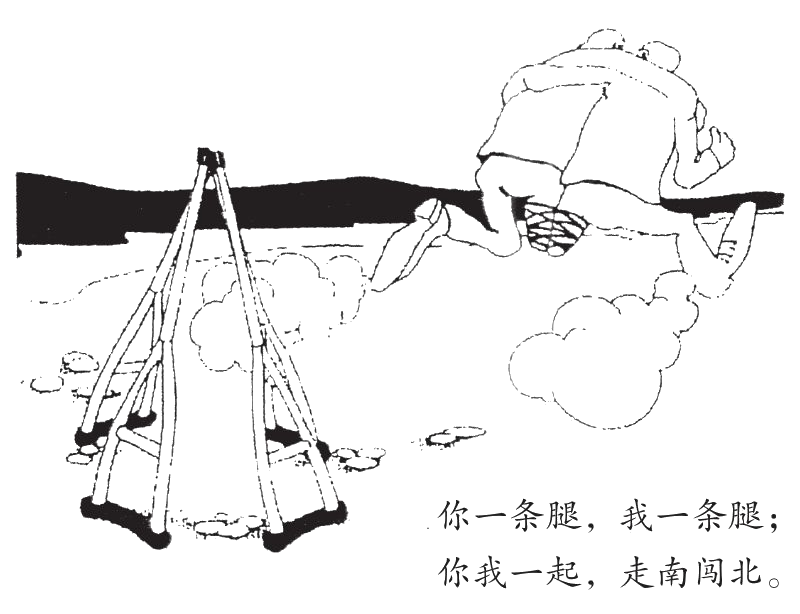
\includegraphics[width=0.54\linewidth]{picture/2008.png}
\end{figure}

%

\bta{2009}




\section{Use of English}

\noindent
\textbf{Directions:}\\
Read the following text. Choose the best word (s) for each numbered blank
and mark A, B, C or D on ANSWER SHEET 1. (10 points)




\TiGanSpace


Research on animal intelligence always makes me wonder just how smart
humans are. \cloze the fruit-fly experiments described by Carl
Zimmer in the \emph{Science Times}. Fruit flies who were taught to be
smarter than the average fruit fly \cloze to live shorter lives.
This suggests that \cloze bulbs burn longer, that there is
a(n) \cloze in not being too bright.


Intelligence, it \cloze , is a high-priced option. It takes more
upkeep, burns more fuel and is slow \cloze the starting line
because it depends on learning --- a(n) \cloze process--- instead
of instinct. Plenty of other species are able to learn, and one of the
things they've apparently learned is when to \cloze.

Is there an adaptive value to \cloze intelligence? That's the
question behind this new research. Instead of casting a wistful
glance \cloze at all the species we've left in the dust
I.Q.-wise, it implicitly asks what the real \cloze of our own
intelligence might be. This is \cloze the mind of every animal
we've ever met.

Research on animal intelligence also makes us wonder what experiments
animals would \cloze on humans if they had the chance. Every cat
with an owner, \cloze , is running a small-scale study in
operant conditioning. We believe that \cloze animals ran the
labs, they would test us to \cloze the limits of our patience,
our faithfulness, our memory for locations. They would try to decide
what intelligence in humans is really \cloze , not merely how
much of it there is. \cloze , they would hope to study
a(n) \cloze question: Are humans actually aware of the world
they live in? \cloze the results are inconclusive.




\newpage


\begin{enumerate}
	%\renewcommand{\labelenumi}{\arabic{enumi}.}
	% A(\Alph) a(\alph) I(\Roman) i(\roman) 1(\arabic)
	%设定全局标号series=example	%引用全局变量resume=example
	%[topsep=-0.3em,parsep=-0.3em,itemsep=-0.3em,partopsep=-0.3em]
	%可使用leftmargin调整列表环境左边的空白长度 [leftmargin=0em]
	\item

\fourchoices
{Suppose}
{Consider}
{Observe}
{Imagine}




\item


\fourchoices
{tended}
{feared}
{happened}
{threatened}




\item


\fourchoices
{thinner}
{stabler}
{lighter}
{dimmer}




\item

\fourchoices
{tendency}
{advantage}
{inclination}
{priority}




\item


\fourchoices
{insists on}
{sums up}
{turns out}
{puts forward}





\item


\fourchoices
{off}
{behind}
{over}
{along}




\item

\fourchoices
{incredible}
{spontaneous}
{inevitable}
{gradual}


\item


\fourchoices
{fight}
{doubt}
{stop}
{think}




\item


\fourchoices
{invisible}
{limited}
{indefinite}
{different}




\item


\fourchoices
{upward}
{forward}
{afterward}
{backward}




\item


\fourchoices
{features}
{influences}
{results}
{costs}




\item


\fourchoices
{outside}
{on}
{by}
{across}




\item


\fourchoices
{deliver}
{carry}
{perform}
{apply}




\item


\fourchoices
{by chance}
{in contrast}
{as usual}
{for instance}





\item


\fourchoices
{if}
{unless}
{as}
{lest}




\item


\fourchoices
{moderate}
{overcome}
{determine}
{reach}




\item


\fourchoices
{at}
{for}
{after}
{with}




\item


\fourchoices
{Above all}
{After all}
{However}
{Otherwise}




\item

\fourchoices
{fundamental}
{comprehensive}
{equivalent}
{hostile}




\item


\fourchoices
{By accident}
{In time}
{So far}
{Better still}



\end{enumerate}


\vfil

\section{Reading Comprehension}



\noindent
\textbf{Part A}\\
\textbf{Directions:}\\
Read the following four texts. Answer the questions below each
text by choosing A, B, C or
D. Mark your answers
on ANSWER SHEET 1. (40 points)


\newpage
\subsection{Text 1}


Habits are a funny thing. We reach for them mindlessly, setting our
brains on auto-pilot and relaxing into the unconscious comfort of
familiar routine. ``Not choice, but habit rules the unreflecting herd,''
William Wordsworth said in the 19th century. In the ever-changing 21 st
century, even the word ``habit'' carries a negative implication.

So it seems paradoxical to talk about habits in the same context as
creativity and innovation. But brain researchers have discovered that
when we consciously develop new habits, we create parallel paths, and
even entirely new brain cells, that can jump our trains of thought onto
new, innovative tracks.

Rather than dismissing ourselves as unchangeable creatures of habit, we
can instead direct our own change by consciously developing new habits.
In fact, the more new things we try --- the more we step outside our
comfort zone --- the more inherently creative we become, both in the
workplace and in our personal lives.

But don't bother trying to kill off old habits; once
those \uline{ruts} of procedure are worn into the brain, they're
there to stay. Instead, the new habits we deliberately press into
ourselves create parallel pathways that can bypass those old roads.

``The first thing needed for innovation is a fascination with wonder,''
says Dawna Markova, author of \emph{The Open Mind}. ``But we are taught
instead to `decide', just as our president calls himself `the Decider.'
'' She adds, however, that ``to decide is to kill off all possibilities
but one. A good innovational thinker is always exploring the many other
possibilities.''

All of us work through problems in ways of which we're unaware, she
says. Researchers in the late 1960s discovered that humans are born with
the capacity to approach challenges in four primary ways: analytically,
procedurally, relationally (or collaboratively) and innovatively. At the
end of adolescence, however, the brain shuts down half of that capacity,
preserving only those modes of thought that have seemed most valuable
during the first decade or so of life.

The current emphasis on standardized testing highlights analysis and
procedure, meaning that few of us inherently use our innovative and
collaborative modes of thought. ``This breaks the major rule in the
American belief system---that anyone can do anything,'' explains M. J.
Ryan, author of the 2006 book \emph{This Year I Will...} and Ms.
Markova's business partner. ``That's a lie that we have perpetuated, and
it fosters commonness. Knowing what you're good at and doing even more
of it creates excellence.'' This is where developing new habits comes
in.


\begin{enumerate}[resume]
	%\renewcommand{\labelenumi}{\arabic{enumi}.}
	% A(\Alph) a(\alph) I(\Roman) i(\roman) 1(\arabic)
	%设定全局标号series=example	%引用全局变量resume=example
	%[topsep=-0.3em,parsep=-0.3em,itemsep=-0.3em,partopsep=-0.3em]
	%可使用leftmargin调整列表环境左边的空白长度 [leftmargin=0em]
	\item
 In Wordsworth's view, ``habits'' is characterized by being \lineread.



\fourchoices
{casual}
{familiar}
{mechanical}
{changeable.}




\item
Brain researchers have discovered that the formation of
habit can be \lineread.



\fourchoices
{predicted}
{regulated}
{traced}
{guided}




\item
The word ``ruts''(Line 1, Paragraph 4) is closest in meaning to \lineread.


\fourchoices
{tracks}
{series}
{characteristics}
{connections}



\item
 Dawna Markova would most probably agree that \lineread.


\fourchoices
{ideas are born of a relaxing mind}
{innovativeness could be taught}
{decisiveness derives from fantastic ideas}
{curiosity activates creative minds}



\item
 Ryan's comments suggest that the practice of standardized
testing \lineread.


\fourchoices
{prevents new habits from being formed}
{no longer emphasizes commonness}
{maintains the inherent American thinking model}
{complies with the American belief system}


\end{enumerate}



\newpage
\subsection{Text 2}


It is a wise father that knows his own child, but today a man can boost
his paternal (fatherly) wisdom---or at least confirm that he's the
kid's dad. All he needs to do is shell out \$30 for paternity testing
kit (PTK) at his local drugstore---and another \$120 to get the
results.

More than 60,000 people have purchased the PTKs since they first become
available without prescriptions last years, according to Doug Fogg,
chief operating officer of Identigene, which makes the over-the-counter
kits. More than two dozen companies sell DNA tests directly to the
public, ranging in price from a few hundred dollars to more than \$2500.

Among the most popular: paternity and kinship testing, which adopted
children can use to find their biological relatives and families can use
to track down kids put up for adoption. DNA testing is also the latest
rage among passionate genealogists---and supports businesses that
offer to search for a family's geographic roots.

Most tests require collecting cells by swabbing saliva in the mouth and
sending it to the company for testing. All tests require a potential
candidate with whom to compare DNA.

But some observers are skeptical. ``There is a kind of false precision
being hawked by people claiming they are doing ancestry testing,'' says
Troy Duster, a New York University sociologist. He notes that each
individual has many ancestors---numbering in the hundreds just a few
centuries back. Yet most ancestry testing only considers a single
lineage, either the Y chromosome inherited through men in a father's
line or mitochondrial DNA, which is passed down only from mothers. This
DNA can reveal genetic information about only one or two ancestors, even
though, for example, just three generations back people also have six
other great-grandparents or, four generations back, 14 other
great-great-grandparents.

Critics also argue that commercial genetic testing is only as good as
the reference collections to which a sample is compared. Databases used
by some companies don't rely on data collected systematically but rather
lump together information from different research projects. This means
that a DNA database may have a lot of data from some regions and not
others, so a person's test results may differ depending on the company
that processes the results. In addition, the computer programs a company
uses to estimate relationships may be patented and not subject to peer
review or outside evaluation.


\begin{enumerate}[resume]
	%\renewcommand{\labelenumi}{\arabic{enumi}.}
	% A(\Alph) a(\alph) I(\Roman) i(\roman) 1(\arabic)
	%设定全局标号series=example	%引用全局变量resume=example
	%[topsep=-0.3em,parsep=-0.3em,itemsep=-0.3em,partopsep=-0.3em]
	%可使用leftmargin调整列表环境左边的空白长度 [leftmargin=0em]
	\item
 In paragraphs 1 and 2, the text shows PTK's \lineread.


\fourchoices
{easy availability}
{flexibility in pricing}
{successful promotion}
{popularity with households}



\item
 PTK is used to \lineread.


\fourchoices
{locate one's birth place}
{promote genetic research}
{identify parent-child kinship}
{choose children for adoption}



\item
Skeptical observers believe that ancestry testing fails
to \lineread.


\fourchoices
{trace distant ancestors}
{rebuild reliable bloodlines}
{fully use genetic information}
{achieve the claimed accuracy}


\item
 In the last paragraph, a problem commercial genetic testing
faces is \lineread.


\fourchoices
{disorganized data collection}
{overlapping database building}
{excessive sample comparison}
{lack of patent evaluation}



\item
An appropriate title for the text is most likely to
be \lineread.


\fourchoices
{Fors and Againsts of DNA Testing}
{DNA Testing and Its Problems}
{DNA Testing Outside the Lab}
{Lies Behind DNA Testing}


\end{enumerate}


\newpage
\subsection{Text 3}

\newlinespread{1.26}{
The relationship between formal education and economic growth in poor
countries is widely misunderstood by economists and politicians alike.
Progress in both areas is undoubtedly necessary for the social,
political, and intellectual development of these and all other
societies; however, the conventional view that education should be one
of the very highest priorities for promoting rapid economic development
in poor countries is wrong. We are fortunate that it is, because
building new educational systems there and putting enough people through
them to improve economic performance would require two or three
generations. The findings of a research institution have consistently
shown that workers in all countries can be trained on the job to achieve
radically higher productivity and, as a result, radically higher
standards of living.

Ironically, the first evidence for this idea appeared in the United
States. Not long ago, with the country entering a recession and Japan at
its pre-bubble peak, the U.S. workforce was derided as poorly educated
and one of primary causes of the poor U.S. economic performance. Japan
was, and remains, the global leader in automotive-assembly productivity.
Yet the research revealed that the U.S. factories of Honda, Nissan, and
Toyota achieved about 95 percent of the productivity of their Japanese
counterparts---a result of the training that U.S. workers received on
the job.

More recently, while examining housing construction, the researchers
discovered that illiterate, non-English-speaking Mexican workers in
Houston, Texas, consistently met best-practice labor productivity
standards despite the complexity of the building industry's work.

What is the real relationship between education and economic
development? We have to suspect that continuing economic growth promotes
the development of education even when governments don't force it. After
all, that's how education got started. When our ancestors were hunters
and gatherers 10, 000 years ago, they didn't have time to wonder much
about anything besides finding food. Only when humanity began to get its
food in a more productive way was there time for other things.

As education improved, humanity's productivity potential increased as
well. When the competitive environment pushed our ancestors to achieve
that potential, they could in turn afford more education. This
increasingly high level of education is probably a necessary, but not a
sufficient, condition for the complex political systems required by
advanced economic performance. Thus poor countries might not be able to
escape their poverty traps without political changes that may be
possible only with broader formal education. A lack of formal education,
however, doesn't constrain the ability of the developing world's
workforce to substantially improve productivity for the foreseeable
future. On the contrary, constraints on improving productivity explain
why education isn't developing more quickly there than it is.


\begin{enumerate}[resume,]
	%\renewcommand{\labelenumi}{\arabic{enumi}.}
	% A(\Alph) a(\alph) I(\Roman) i(\roman) 1(\arabic)
	%设定全局标号series=example	%引用全局变量resume=example
	%[topsep=-0.3em,parsep=-0.3em,itemsep=-0.3em,partopsep=-0.3em]
	%可使用leftmargin调整列表环境左边的空白长度 [leftmargin=0em]
	\item
The author holds in paragraph 1 that the importance of
education in poor countries \lineread.


\fourchoices
{is subject to groundless doubts}
{has fallen victim of bias}
{is conventionally downgraded}
{has been overestimated}



\item
 It is stated in paragraph 1 that the construction of a new
education system \lineread.


\fourchoices
{challenges economists and politicians}
{takes efforts of generations}
{demands priority from the government}
{requires sufficient labor force}



\item
 A major difference between the Japanese and U. S workforces
is that \lineread.


\fourchoices
{the Japanese workforce is better disciplined}
{the Japanese workforce is more productive}
{the U. S workforce has a better education}
{the U. S workforce is more organize}



\item
The author quotes the example of our ancestors to show that
education emerged \lineread.


\fourchoices
{when people had enough time}
{prior to better ways of finding food}
{when people on longer went hungry}
{as a result of pressure on government}



\item
According to the last paragraph, development of education \lineread.


\fourchoices
{results directly from competitive environments}
{does not depend on economic performance}
{follows improved productivity}
{cannot afford political changes}

\end{enumerate}
}


\newpage
\subsection{Text 4}


The most thoroughly studied intellectuals in the history of the New
World are the ministers and political leaders of seventeenth-century New
England. According to the standard history of American philosophy,
nowhere else in colonial America was ``so much importance attached to
intellectual pursuits.'' According to many books and articles, New
England's leaders established the basic themes and preoccupations of an
unfolding, dominant Puritan tradition in American intellectual life.

To take this approach to the New Englanders normally means to start with
the Puritans' theological innovations and their distinctive ideas about
the church---important subjects that we may not neglect. But in keeping
with our examination of southern intellectual life, we may consider the
original Puritans as carriers of European culture, adjusting to New
World circumstances. The New England colonies were the scenes of
important episodes in the pursuit of widely understood ideals of
civility and virtuosity.

The early settlers of Massachusetts Bay included men of impressive
education and influence in England. Besides the ninety or so learned
ministers who came to Massachusetts churches in the decade after 1629,
there were political leaders like John Winthrop, an educated gentleman,
lawyer, and official of the Crown before he journeyed to Boston. These
men wrote and published extensively, reaching both New World and Old
World audiences, and giving New England an atmosphere of intellectual
earnestness.

We should not forget, however, that most New Englanders were less well
educated. While few craftsmen or farmers, let alone dependents and
servants, left literary compositions to be analyzed, it is obvious that their views were less fully intellectualized.
Their thinking often had a traditional superstitious quality. A tailor named John Dane,
who emigrated in the late 1630 s, left an account of his reasons for
leaving England that is filled with signs. Sexual confusion, economic
frustrations, and religious hope-all name together in a decisive moment
when he opened the Bible, told his father that the first line he saw
would settle his fate, and read the magical words: ``Come out from among
them, touch no unclean thing, and I will be your God and you shall be my
people.'' One wonders what Dane thought of the careful sermons
explaining the Bible that he heard in Puritan churches.

Meanwhile, many settles had slighter religious commitments than Dane's,
as one clergyman learned in confronting folk along the coast who mocked
that they had not come to the New World for religion. ``Our main end was
to catch fish.''


\begin{enumerate}[resume]
	%\renewcommand{\labelenumi}{\arabic{enumi}.}
	% A(\Alph) a(\alph) I(\Roman) i(\roman) 1(\arabic)
	%设定全局标号series=example	%引用全局变量resume=example
	%[topsep=-0.3em,parsep=-0.3em,itemsep=-0.3em,partopsep=-0.3em]
	%可使用leftmargin调整列表环境左边的空白长度 [leftmargin=0em]
	\item
 The author notes that in the seventeenth-century New
England \lineread.


\fourchoices
{Puritan tradition dominated political life}
{intellectual interests were encouraged}
{politics benefited much from intellectual endeavors}
{intellectual pursuits enjoyed a liberal environment}



\item
 It is suggested in paragraph 2 that New
Englanders \lineread.


\fourchoices
{experienced a comparatively peaceful early history}
{brought with them the culture of the Old World}
{paid little attention to southern intellectual life}
{were obsessed with religious innovations}



\item
The early ministers and political leaders in Massachusetts
Bay \lineread.


\fourchoices
{were famous in the New World for their writings}
{gained increasing importance in religious affairs}
{abandoned high positions before coming to the New World}
{created a new intellectual atmosphere in New England}



\item
The story of John Dane shows that less well-educated New
Englanders were often \lineread.


\fourchoices
{influenced by superstitions}
{troubled with religious beliefs}
{puzzled by church sermons}
{frustrated with family earnings}


\item
The text suggests that early settlers in New
England \lineread.


\fourchoices
{were mostly engaged in political activities}
{were motivated by an illusory prospect}
{came from different intellectual backgrounds}
{left few formal records for later reference}


\end{enumerate}


\newpage
\noindent
\textbf{Part B}\\
\textbf{Directions}:\\
In the following text, some segments have been removed. For Questions
41-45, choose the most suitable one from the list A-G to fit into each
of the numbered blanks. There are two extra choices, which do not fit in
any of the blanks. Mark your answers on ANSWER SHEET 1. (10 points)



\TiGanSpace


Coinciding with the groundbreaking theory of biological evolution
proposed by British
naturalist Charles Darwin in the 1860s, British social
philosopher Herbert
Spencer put forward his own theory of biological and cultural
evolution. Spencer argued that all worldly phenomena, including human
societies, changed over time, advancing toward perfection. \linefill

American social
scientist Lewis
Henry Morgan introduced another theory of cultural evolution in the
late 1800 s. Morgan helped found modern anthropology---the scientific
study of human societies, customs and beliefs---thus becoming one of the
earliest anthropologists. In his work, he attempted to show how all
aspects of culture changed together in the evolution of societies. \linefill

In the early 1900s in North America, German-born American
anthropologist Franz
Boas developed a new theory of culture known as historical
particularism. Historical particularism, which emphasized the uniqueness
of all cultures, gave new direction to anthropology. \linefill

Boas felt that the culture of any society must be understood as the
result of a unique history and not as one of many cultures belonging to
a broader evolutionary stage or type of culture. \linefill

Historical particularism became a dominant approach to the study of
culture in American anthropology, largely through the influence of many
students of Boas. But a number of anthropologists in the early 1900s
also rejected the particularist theory of culture in favor of
diffusionism. Some attributed virtually every important cultural
achievement to the inventions of a few, especially gifted peoples that,
according to diffusionists, then spread to other cultures. \linefill

Also in the early 1900 s, French
sociologist Emile
Durkheim developed a theory of culture that would greatly influence
anthropology. Durkheim proposed that religious beliefs functioned to
reinforce social solidarity. An interest in the relationship between the
function of society and culture---known as functionalism---became a major theme in European, and
especially British, anthropology.

\begin{listmatch}
	%\renewcommand{\labelenumi}{\arabic{enumi}.}
	% A(\Alph) a(\alph) I(\Roman) i(\roman) 1(\arabic)
	%设定全局标号series=example	%引用全局变量resume=example
	%[topsep=-0.3em,parsep=-0.3em,itemsep=-0.3em,partopsep=-0.3em]
	%可使用leftmargin调整列表环境左边的空白长度 [leftmargin=0em]
	\item
Other anthropologists believed that cultural innovations, such
as inventions, had a single origin and passed from society to society.
This theory was known as diffusionism.


\item 
In order to study particular cultures as completely as possible,
he became skilled
in linguistics,
the study of languages, and in physical anthropology, the study of human
biology and anatomy.


\item 
 He argued that human evolution was characterized by a struggle
he called the ``survival of the fittest,'' in which weaker races and
societies must eventually be replaced by stronger, more advanced races
and societies.


\item 
They also focused on important rituals that appeared to preserve
a people's social structure, such as initiation ceremonies that formally
signify children's entrance into adulthood.


\item 
Thus, in his view, diverse aspects of culture, such as the
structure of families, forms of marriage, categories of kinship,
ownership of property, forms of government, technology, and systems of
food production, all changed as societies evolved.


\item 
Supporters of the theory viewed culture as a collection of
integrated parts that work together to keep a society functioning.


\item 
For example, British anthropologists Grafton Elliot Smith and W.
J. Perry incorrectly suggested, on the basis of inadequate information,
that farming, pottery making, and metallurgy all originated in ancient
Egypt and diffused throughout the world. In fact, all of these cultural
developments occurred separately at different times in many parts of the
world.


\end{listmatch}



\newpage

\noindent
\textbf{Part C}\\
\textbf{Directions:}\\
Read the following text carefully and then translate the underlined
segments into Chinese. Your translation should be written carefully on
\textbf{ANSWER SHEET 2}. (10 points)



\TiGanSpace


There is a marked difference between the education which every one gets
from living with others, and the deliberate educating of the young. In
the former case the education is incidental; it is natural and
important, but it is not the express reason of the association.
\transnum \uline{It may be said that the measure of the worth of any
social institution is its effect in enlarging and improving experience,
but this effect is not a part of its original motive.} Religious
associations began, for example, in the desire to secure the favor of
overruling powers and to ward off evil influences; family life in the
desire to gratify appetites and secure family perpetuity; systematic
labor, for the most part, because of enslavement to others, etc.
\transnum \uline{Only gradually was the by-product of the institution
noted, and only more gradually still was this effect considered as a
directive factor in the conduct of the institution.} Even today, in our
industrial life, apart from certain values of industriousness and
thrift, the intellectual and emotional reaction of the forms of human
association under which the world's work is carried on receives little
attention as compared with physical output.

But in dealing with the young, the fact of association itself as an
immediate human fact, gains in importance. \transnum \uline{While it is
easy to ignore in our contact with them the effect of our acts upon
their disposition, it is not so easy as in dealing with adults.} The
need of training is too evident and the pressure to accomplish a change
in their attitude and habits is too urgent to leave these consequences
wholly out of account. \transnum \uline{Since our chief business with them
is to enable them to share in a commonlife we cannot help considering
whether or not we are forming the powers which will secure this
ability.} If humanity has made some headway in realizing that the
ultimate value of every institution is its distinctively human effect we
may well believe that this lesson has been learned largely through
dealings with the young.

\transnum \uline{We are thus led to distinguish, within the broad
educational process which we have been so far considering, a more formal
kind of education---that of direct tuition or
schooling.} In undeveloped social groups, we find very little formal
teaching and training. These groups mainly rely for instilling needed
dispositions into the young upon the same sort of association which
keeps adults loyal to their group.



\newpage

\section{Writing}


\noindent
\textbf{Part A}\\
\textbf{51. Directions:}

Restrictions on the use of plastic bags have not been so successful in
some regions. ``White Pollution'' is still going on.
Write a letter to the editor (s) of your local newspaper to
\begin{listwrite}
	%\renewcommand{\labelenumi}{\arabic{enumi}.}
	% A(\Alph) a(\alph) I(\Roman) i(\roman) 1(\arabic)
	%设定全局标号series=example	%引用全局变量resume=example
	%[topsep=-0.3em,parsep=-0.3em,itemsep=-0.3em,partopsep=-0.3em]
	%可使用leftmargin调整列表环境左边的空白长度 [leftmargin=0em]
	\item
give your opinions briefly, and

\item 
 make two or three suggestions
\end{listwrite}

You should write about 100 words on ANSWER SHEET 2.

\textbf{Do not} sign your ow name at the end of the letter. Use ``Li Ming'' instead. 

\textbf{Do not} write the
address. (10 points)


\vspace{2em}

\noindent
\textbf{Part B}\\
\textbf{52. Directions:}

Write an essay of 160-200 words based on the following drawing. In your
essay, you should
\begin{listwrite}
	%\renewcommand{\labelenumi}{\arabic{enumi}.}
	% A(\Alph) a(\alph) I(\Roman) i(\roman) 1(\arabic)
	%设定全局标号series=example	%引用全局变量resume=example
	%[topsep=-0.3em,parsep=-0.3em,itemsep=-0.3em,partopsep=-0.3em]
	%可使用leftmargin调整列表环境左边的空白长度 [leftmargin=0em]
	\item
 describe the drawing briefly,

\item 
 explain its intended meaning, and then

\item 
 give your comments.
\end{listwrite}

You should write neatly on ANSHWER SHEET 2. (20 points)


\begin{figure}[h!]
	\centering
	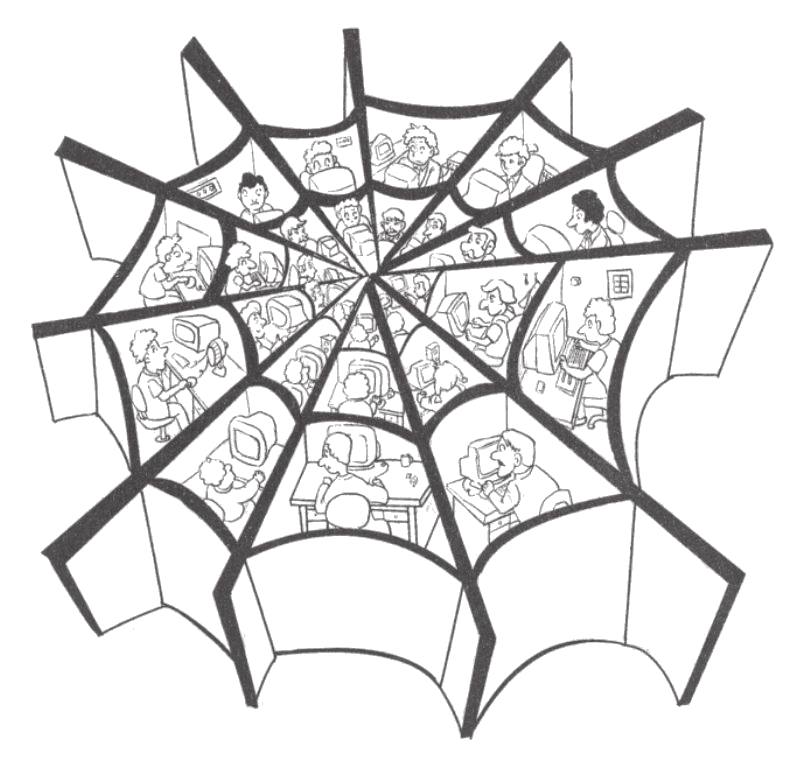
\includegraphics[width=0.32\linewidth]{picture/2009.png}
	\caption*{网络的“近”与“远”}
\end{figure}


\checkpagenumber%

\bta{2010}


\section{Use of English}

\noindent
\textbf{Directions:}\\
Read the following text. Choose the best word (s) for each numbered
blank and mark A, B, C or D on \textbf{ANSWER
	SHEET 1}. (10 points)


\TiGanSpace


In 1924 America's National Research Council sent two engineers to
supervise a series of industrial experiments at a large telephone-parts
factory called the Hawthorne Plant near Chicago. It hoped they would
learn how shop-floor lighting \cloze workers' productivity.
Instead, the studies ended \cloze giving their name to the
``Hawthorne effect'', the extremely influential idea that the very
\cloze of being experimented upon changed subjects' behavior.

The idea arose because of the \cloze behavior of the women in the
Hawthorne plant. According to \cloze of the experiments, their
hourly output rose when lighting was increased, but also when it was
dimmed. It did not \cloze what was done in the experiment;
\cloze something was changed, productivity rose. A(n)
\cloze that they were being experimented upon seemed to be
\cloze to alter workers' behavior \cloze itself.

After several decades, the same data were \cloze to econometric
the analysis. The Hawthorne experiments has another surprise store.
\cloze the descriptions on record, no systematic \cloze
was found that levels of productivity were related to changes in
lighting.

It turns out that peculiar way of conducting the experiments may be have
let to \cloze interpretation of what happened. \cloze ,
lighting was always changed on a Sunday. When work started again on
Monday, output \cloze rose compared with the previous Saturday
and \cloze to rise for the next couple of days. \cloze ,
a comparison with data for weeks when there was no experimentation
showed that output always went up on Monday, Workers \cloze to
be diligent for the first few days of the week in any case, before
\cloze a plateau and then slackening off. This suggests that the
alleged ``Hawthorne effect'' is hard to pin down.


\newpage
\begin{enumerate}
	%\renewcommand{\labelenumi}{\arabic{enumi}.}
	% A(\Alph) a(\alph) I(\Roman) i(\roman) 1(\arabic)
	%设定全局标号series=example	%引用全局变量resume=example
	%[topsep=-0.3em,parsep=-0.3em,itemsep=-0.3em,partopsep=-0.3em]
	%可使用leftmargin调整列表环境左边的空白长度 [leftmargin=0em]
	\item


\fourchoices
{affected}
{achieved}
{extracted}
{restored}




\item


\fourchoices
{at}
{up}
{with}
{off}




\item


\fourchoices
{truth}
{sight}
{act}
{proof}




\item

\fourchoices
{controversial}
{perplexing}
{mischievous}
{ambiguous}


\item

\fourchoices
{requirements}
{explanations}
{accounts}
{assessments}



\item


\fourchoices
{conclude}
{matter}
{indicate}
{work}




\item

\fourchoices
{as far as}
{for fear that}
{in case that}
{so long so}



\item

\fourchoices
{awareness}
{expectation}
{sentiment}
{illusion}


\item


\fourchoices
{suitable}
{excessive}
{enough}
{abundant}




\item


\fourchoices
{about}
{for}
{on}
{by}




\item


\fourchoices
{compared}
{shown}
{subjected}
{conveyed}




\item

\fourchoices
{Contrary to}
{Consistent with}
{Parallel with}
{Peculiar to}



\item


\fourchoices
{evidence}
{guidance}
{implication}
{source}




\item

\fourchoices
{disputable}
{enlightening}
{reliable}
{misleading}



\item

\fourchoices
{In contrast}
{For example}
{In consequence}
{As usual}



\item

\fourchoices
{duly}
{accidentally}
{unpredictably}
{suddenly}



\item


\fourchoices
{failed}
{ceased}
{started}
{continued}




\item

\fourchoices
{Therefore}
{Furthermore}
{However}
{Meanwhile}



\item


\fourchoices
{attempted}
{tended}
{chose}
{intended}




\item


\fourchoices
{breaking}
{climbing}
{surpassing}
{hitting}

\end{enumerate}




\section{Reading Comprehension}



\noindent
\textbf{Part A}\\
\textbf{Directions:}\\
Read the following four texts. Answer the questions below each text by
choosing A, B, C or
D. Mark your answers on
\textbf{ANSWER SHEET 1}. (40 points)



\subsection{Text 1}


Of all the changes that have taken place in English-language newspapers
during the past quarter-century, perhaps the most far-reaching has been
the inexorable decline in the scope and seriousness of their arts
coverage.

It is difficult to the point of impossibility for the average reader
under the age of forty to imagine a time when high-quality arts
criticism could be found in most big-city newspapers. Yet a considerable
number of the most significant collections of criticism published in the
20th century consisted in large part of newspaper
reviews. To read such books today is to marvel at the fact that their
learned contents were once deemed suitable for publication in
general-circulation dailies.

We are even farther removed from the unfocused newspaper reviews
published in England between the turn of the 20th
century and the eve of World War II, at a time when newsprint was
dirt-cheap and stylish arts criticism was considered an ornament to the
publications in which it appeared. In those far-off days, it was taken
for granted that the critics of major papers would write in detail and
at length about the events they covered. Theirs was a serious business,
and even those reviewers who wore their learning lightly, like George
Bernard Shaw and Ernest Newman, could be trusted to know what they were
about. These men believed in journalism as a calling, and were proud to
be published in the daily press. ``So few authors have brains enough or
literary gift enough to keep their own end up in journalism,'' Newman
wrote, ``that I am tempted to define `journalism' as `a term of contempt
applied by writers who are not read to writers who are'.''

Unfortunately, these critics are virtually forgotten. Neville Cardus,
who wrote for the \emph{Manchester Guardian} from 1917 until shortly
before his death in 1975, is now known solely as a writer of essays on
the game of cricket. During his lifetime, though, he was also one of
England's foremost classical-music critics, a stylist so widely admired
that his \emph{Autobiography} (1947) became a best-seller. He was
knighted in 1967, the first music critic to be so honored. Yet only one
of his books is now in print, and his vast body of writings on music is
unknown save to specialists.

Is there any chance that Cardus's criticism will enjoy a revival? The
prospect seems remote. Journalistic tastes had changed long before his
death, and postmodern readers have little use for the richly upholstered
Vicwardian prose in which he specialized. Moreover, the amateur
tradition in music criticism has been in headlong retreat.


\begin{enumerate}[resume]
	%\renewcommand{\labelenumi}{\arabic{enumi}.}
	% A(\Alph) a(\alph) I(\Roman) i(\roman) 1(\arabic)
	%设定全局标号series=example	%引用全局变量resume=example
	%[topsep=-0.3em,parsep=-0.3em,itemsep=-0.3em,partopsep=-0.3em]
	%可使用leftmargin调整列表环境左边的空白长度 [leftmargin=0em]
	\item
It is indicated in Paragraphs 1 and 2 that \lineread.


\fourchoices
{arts criticism has disappeared from big-city newspapers}
{English-language newspapers used to carry more arts reviews}
{high-quality newspapers retain a large body of readers}
{young readers doubt the suitability of criticism on dailies}



\item
 Newspaper reviews in England before World War II were
characterized by \lineread.


\fourchoices
{free themes}
{casual style}
{elaborate layout}
{radical viewpoints}



\item
Which of the following would Shaw and Newman most probably
agree on?


\fourchoices
{It is writers' duty to fulfill journalistic goals.}
{It is contemptible for writers to be journalists.}
{Writers are likely to be tempted into journalism.}
{Not all writers are capable of journalistic writing.}



\item
 What can be learned about Cardus according to the last two
paragraphs?


\fourchoices
{His music criticism may not appeal to readers today.}
{His reputation as a music critic has long been in dispute.}
{His style caters largely to modern specialists.}
{His writings fail to follow the amateur tradition.}



\item
What would be the best title for the text?


\fourchoices
{Newspapers of the Good Old Days}
{The Lost Horizon in Newspapers}
{Mournful Decline of Journalism}
{Prominent Critics in Memory}

\end{enumerate}


\newpage
\subsection{Text 2}


Over the past decade, thousands of patents have been granted for what
are called business methods. Amazon.com received one for its  ``one-click''
online payment system. Merrill Lynch got legal protection for an asset
allocation strategy. One inventor patented a technique for lifting a
box.

Now the nation's top patent court appears completely ready to scale back
on business-method patents, which have been controversial ever since
they were first authorized 10 years ago. In a move that has
intellectual-property lawyers abuzz, the U.S. Court of Appeals for the Federal Circuit said
it would use a particular case to conduct a broad
review of business-method patents.  \emph{In re Bilski}, as the case is
known , is ``a very big deal'', says Dennis
D. Crouch of the University of
Missouri School of Law. It " has the potential to eliminate an entire
class of patents."

Curbs on business-method claims would be a dramatic \uline{about-face}, because
it was the Federal Circuit itself that introduced such patents with is
1998 decision in the so-called State Street Bank case, approving a
patent on a way of pooling mutual-fund assets. That ruling produced an
explosion in business-method patent filings, initially by emerging
Internet companies trying to stake out exclusive rights to specific
types of online transactions. Later, move established companies raced to
add such patents to their files, if only as a defensive move against
rivals that might beat them to the punch. In 2005, IBM noted in a court
filing that it had been issued more than 300 business-method patents,
despite the fact that it questioned the legal basis for granting them.
Similarly, some Wall Street investment films armed themselves with
patents for financial products, even as they took positions in court
cases opposing the practice.

The Bilski case involves a claimed patent on a method for hedging risk
in the energy market. The Federal Circuit issued an unusual order
stating that the case would be heard by all 12 of the court's judges,
rather than a typical panel of three, and that one issue it wants to
evaluate is whether it should ``reconsider'' its State Street Bank ruling.

The Federal Circuit's action comes in the wake of a series of recent
decisions by the Supreme Court that has narrowed the scope of
protections for patent holders. Last April, for example the justices
signaled that too many patents were being upheld for ``inventions'' that
are obvious. The judges on the Federal Circuit are ``reacting to the
anti-patent trend at the Supreme Court'', says Harold C. Wegner, a patent
attorney and professor at George Washington University Law School.


\begin{enumerate}[resume]
	%\renewcommand{\labelenumi}{\arabic{enumi}.}
	% A(\Alph) a(\alph) I(\Roman) i(\roman) 1(\arabic)
	%设定全局标号series=example	%引用全局变量resume=example
	%[topsep=-0.3em,parsep=-0.3em,itemsep=-0.3em,partopsep=-0.3em]
	%可使用leftmargin调整列表环境左边的空白长度 [leftmargin=0em]
	\item
Business-method patents have recently aroused concern
because of \lineread.

\fourchoices
{their limited value to business}
{their connection with asset allocation}
{the possible restriction on their granting}
{the controversy over authorization}



\item
Which of the following is true of the Bilski case?

\fourchoices
{Its ruling complies with the court decisions.}
{It involves a very big business transaction.}
{It has been dismissed by the Federal Circuit.}
{It may change the legal practices in the U.S.}


\item
The word ``about-face'' (Line 1, Para 3) most probably
means \lineread.
\fourchoices
{loss of good will}
{increase of hostility}
{change of attitude}
{enhancement of dignity}



\item
We learn from the last two paragraphs that business-method
patents \lineread.

\fourchoices
{are immune to legal challenges}
{are often unnecessarily issued}
{lower the esteem for patent holders}
{increase the incidence of risks}



\item
Which of the following would be the subject of the text?

\fourchoices
{A looming threat to business-method patents}
{Protection for business-method patent holders}
{A legal case regarding business-method patents}
{A prevailing trend against business-method patents}


\end{enumerate}


\newpage
\subsection{Text 3}


In his book \emph{The Tipping Point}, Malcolm Gladwell argues that ``social
epidemics'' are driven in large part by the acting of a tiny minority of
special individuals, often called influentials, who are unusually
informed, persuasive, or well-connected. The idea is intuitively
compelling, but it doesn't explain how ideas actually spread.

The supposed importance of influentials derives from a
plausible-sounding but largely untested theory called the " two-step
flow of communication": Information flows from the media to the
influentials and from them to everyone else. Marketers have embraced the
two-step flow because it suggests that if they can just find and
influence the influentials, those selected people will do most of the
work for them. The theory also seems to explain the sudden and
unexpected popularity of certain looks, brands, or neighborhoods. In
many such cases, a cursory search for causes finds that some small group
of people was wearing, promoting, or developing whatever it is before
anyone else paid attention. Anecdotal evidence of this kind fits nicely
with the idea that only certain special people can drive trends.

In their recent work, however, some researchers have come up with the
finding that influentials have far less impact on social epidemics than
is generally supposed. In fact, they don't seem to be required at all.

The researchers' argument stems from a simple observing about social
influence: With the exception of a few celebrities like Oprah
Winfrey---whose outsize presence is primarily a function of media, not
interpersonal, influence---even the most influential members of a
population simply don't interact with that many others. Yet it is
precisely these non-celebrity influentials who, according to the
two-step-flow theory, are supposed to drive social epidemics, by
influencing their friends and colleagues directly. For a social epidemic
to occur, however, each person so affected, must then influence his or
her own acquaintances, who must in turn influence theirs, and so on; and
just how many others pay attention to each of \uline{these people} has little to
do with the initial influential. If people in the network just two
degrees removed from the initial influential prove resistant, for
example, the cascade of change won't propagate very far or affect many
people.

Building on the basic truth about interpersonal influence, the
researchers studied the dynamics of social influence by conducting
thousands of computer simulations of populations, manipulating a number
of variables relating to people's ability to influence others and their
tendency to be influenced. They found that the principal requirement for
what is called ``global cascades''---the widespread propagation of
influence through networks---is the presence not of a few influentials
but, rather, of a critical mass of easily influenced people.


\begin{enumerate}[resume]
	%\renewcommand{\labelenumi}{\arabic{enumi}.}
	% A(\Alph) a(\alph) I(\Roman) i(\roman) 1(\arabic)
	%设定全局标号series=example	%引用全局变量resume=example
	%[topsep=-0.3em,parsep=-0.3em,itemsep=-0.3em,partopsep=-0.3em]
	%可使用leftmargin调整列表环境左边的空白长度 [leftmargin=0em]
	\item
By citing the book \emph{The Tipping Point}, the author
	intends to \lineread.


\fourchoices
{analyze the consequences of social epidemics}
{discuss influentials' function in spreading ideas}
{exemplify people's intuitive response to social epidemics}
{describe the essential characteristics of influentials}



\item
 The author suggests that the ``two-step-flow theory'' \lineread.


\fourchoices
{serves as a solution to marketing problems}
{has helped explain certain prevalent trends}
{has won support from influentials}
{requires solid evidence for its validity}


\item 
What the researchers have observed recently shows that \lineread.



\fourchoices
{the power of influence goes with social interactions}
{interpersonal links can be enhanced through the media}
{influentials have more channels to reach the public}
{most celebrities enjoy wide media attention}



\item
The underlined phrase ``these people'' in Paragraph 4 refers
to the ones who \lineread.


\fourchoices
{stay outside the network of social influence}
{have little contact with the source of influence}
{are influenced and then influence others}
{are influenced by the initial influential}


\item
 What is the essential element in the dynamics of social
influence?


\fourchoices
{The eagerness to be accepted.}
{The impulse to influence others.}
{The readiness to be influenced.}
{The inclination to rely on others.}

\end{enumerate}



\newpage
\subsection{Text 4}


Bankers have been blaming themselves for their troubles in public.
Behind the scenes, they have been taking aim at someone else: the
accounting standard-setters. Their rules, moan the banks, have forced
them to report enormous losses, and it's just not fair. These rules say
they must value some assets at the price a third party would pay, not
the price managers and regulators would like them to fetch.

Unfortunately, banks' lobbying now seems to be working. The details may
be unknowable, but the independence of standard-setters, essential to
the proper functioning of capital markets, is being compromised. And,
unless banks carry toxic assets at prices that attract buyers, reviving
the banking system will be difficult.

After a bruising encounter with Congress, America's Financial Accounting
Standards Board (FASB) rushed through rule changes. These gave banks
more freedom to use models to value illiquid assets and more flexibility
in recognizing losses on long-term assets in their income statement. Bob
Herz, the FASB's chairman, cried out against those who ``question our
motives.'' Yet bank shares rose and the changes enhance what one lobby
group politely calls ``the use of judgment by management.''

European ministers instantly demanded that the International Accounting
Standards Board (IASB) do likewise. The IASB says it does not want to
act without overall planning, but the pressure to fold when it completes
it reconstruction of rules later this year is strong. Charlie McCreevy,
a European commissioner, warned the IASB that it did ``not live in a
political vacuum'' but ``'in the real word'' and that Europe could yet
develop different rules.

It was banks that were \uline{on the wrong planet}, with accounts that vastly
overvalued assets. Today they argue that market prices overstate losses,
because they largely reflect the temporary illiquidity of markets, not
the likely extent of bad debts. The truth will not be known for years.
But bank's shares trade below their book value, suggesting that
investors are skeptical. And dead markets partly reflect the paralysis
of banks which will not sell assets for fear of booking losses, yet are
reluctant to buy all those supposed bargains.

To get the system working again, losses must be recognized and dealt
with. America's new plan to buy up toxic assets will not work unless
banks mark assets to levels which buyers find attractive. Successful
markets require independent and even combative standard-setters. The
FASB and IASB have been exactly that, cleaning up rules on stock options
and pensions, for example, against hostility from special interests. But
by giving in to critics now they are inviting pressure to make more
concessions.

\begin{enumerate}[resume]
	%\renewcommand{\labelenumi}{\arabic{enumi}.}
	% A(\Alph) a(\alph) I(\Roman) i(\roman) 1(\arabic)
	%设定全局标号series=example	%引用全局变量resume=example
	%[topsep=-0.3em,parsep=-0.3em,itemsep=-0.3em,partopsep=-0.3em]
	%可使用leftmargin调整列表环境左边的空白长度 [leftmargin=0em]
	\item
Bankers complained that they were forced to \lineread.


\fourchoices
{follow unfavorable asset evaluation rules}
{collect payments from third parties}
{cooperate with the price managers}
{re-evaluate some of their assets}



\item
According to the author, the rule changes of the FASB may
result in \lineread.


\fourchoices
{the diminishing role of management}
{the revival of the banking system}
{the banks' long-term asset losses}
{the weakening of its independence}


\item
According to Paragraph 4, McCreevy objects to the IASB's
attempt to \lineread.


\fourchoices
{keep away from political influences}
{evade the pressure from their peers}
{act on their own in rule-setting}
{take gradual measures in reform}



\item
The author thinks the banks were ``on the wrong planet'' in
that they \lineread.


\fourchoices
{misinterpreted market price indicators}
{exaggerated the real value of their assets}
{neglected the likely existence of bad debts}
{denied booking losses in their sale of assets}



\item
The author's attitude towards standard-setters is one of \lineread.


\fourchoices
{satisfaction}
{skepticism}
{objectiveness}
{sympathy}


\end{enumerate}


\newpage

\noindent
\textbf{Part B}\\
\textbf{Directions:}\\
For Questions 41-45, choose the most suitable paragraphs from the list
A-G and fill them into the numbered boxes to form a coherent text.
Paragraph E has been correctly placed. There is one paragraph which does
not fit in with the text. Mark your answers on \textbf{ANSWER SHEET 1}.
(10 points)

\begin{listmatch}
	%\renewcommand{\labelenumi}{\arabic{enumi}.}
	% A(\Alph) a(\alph) I(\Roman) i(\roman) 1(\arabic)
	%设定全局标号series=example	%引用全局变量resume=example
	%[topsep=-0.3em,parsep=-0.3em,itemsep=-0.3em,partopsep=-0.3em]
	%可使用leftmargin调整列表环境左边的空白长度 [leftmargin=0em]
	\item
The first and more important is the consumer's growing
preference for eating out: the consumption of food and drink in places
other than homes has risen from about 32 percent of total consumption in
1995 to 35 percent in 2000 and is expected to approach 38 percent by
2005. This development is boosting wholesale demand from the food
service segment by 4 to 5 percent a year across Europe, compared with
growth in retail demand of 1 to 2 percent. Meanwhile, as the recession
is looming large, people are getting anxious. They tend to keep a
tighter hold on their purse and consider eating at home a realistic
alternative.


\item 
 Retail sales of food and drink in Europe's largest markets are
at a standstill, leaving European grocery retailers hungry for
opportunities to grow. Most leading retailers have already tried
e-commerce, with limited success, and expansion abroad. But almost all
have ignored the big, profitable opportunity in their own backyard: the
wholesale food and drink trade, which appears to be just the kind of
market retailers need.


\item 
 Will such variations bring about a change in the overall
structure of the food and drink market? Definitely not. The functioning
of the market is based on flexible trends dominated by potential buyers.
In other words, it is up to the buyer, rather than the seller, to decide
what to buy. At any rate, this change will ultimately be acclaimed by an
ever-growing number of both domestic and international consumers,
regardless of how long the current consumer pattern will take hold.


\item 
 All in all, this clearly seems to be a market in which big
retailers could profitably apply their gigantic scale, existing infrastructure
and proven skills in the management of product ranges, logistics, and
marketing intelligence. Retailers that master the intricacies of
wholesaling in Europe may well expect to rake in substantial profits
thereby. At least, that is how it looks as a whole. Closer inspection
reveals important differences among the biggest national markets,
especially in their customer segments and wholesale structures, as well
as the competitive dynamics of individual food and drink categories. Big
retailers must understand these differences before they can identify the
segments of European wholesaling in which their particular abilities
might unseat smaller but entrenched competitors. New skills and
unfamiliar business models are needed too.


\item 
 Despite variations in detail, wholesale markets in the countries
that have been closely examined---France, Germany, Italy, and
Spain---are made out of the same building blocks. Demand comes mainly
from two sources: independent mom-and-pop grocery stores which, unlike
large retail chains, are too small to buy straight from producers, and
food service operators that cater to consumers when they don't eat at
home. Such food service operators range from snack machines to large
institutional catering ventures, but most of these businesses are known
in the trade as ``horeca'': hotels, restaurants, and cafes. Overall,
Europe's wholesale market for food and drink is growing at the same
sluggish pace as the retail market, but the figures, when added
together, mask two opposing trends.


\item 
 For example, wholesale food and drink sales come to \$268
billion in France, Germany, Italy, Spain, and the United Kingdom in
2000---more than 40 percent of retail sales. Moreover, average overall
margins are higher in wholesale than in retail; wholesale demand from
the food service sector is growing quickly as more Europeans eat out
more often; and changes in the competitive dynamics of this fragmented
industry are at last making it feasible for wholesalers to consolidate.


\item 
 However, none of these requirements should deter large retailers
(and even some large food producers and existing wholesalers) from
trying their hand, for those that master the intricacies of wholesaling
in Europe stand to reap considerable gains.
\end{listmatch}


\[ 
\begin{tabular}{|c|c|}
	\hline
	41. &  \hspace{1.5em} \\
	\hline
\end{tabular}
\rightarrow
\begin{tabular}{|c|c|}
	\hline
	42. &  \hspace{1.5em} \\
	\hline
\end{tabular}
\rightarrow
\begin{tabular}{|c|c|}
	\hline
	43. &  \hspace{1.5em} \\
	\hline
\end{tabular}
\rightarrow
\begin{tabular}{|c|c|}
	\hline
	44. &  \hspace{1.5em} \\
	\hline
\end{tabular}
\rightarrow
\begin{tabular}{|c|}
	\hline
	E \\
	\hline
\end{tabular}
\rightarrow
\begin{tabular}{|c|c|}
	\hline
	45. &  \hspace{1.5em} \\
	\hline
\end{tabular}
 \]


\phantom{ \linefill \linefill \linefill \linefill \linefill}


\newpage
\noindent
\textbf{Part C}\\
\textbf{Directions:}\\
Read the following text carefully and then translate the underlined
segments into Chinese. Your translation should be written carefully on
\textbf{ANSWER SHEET 2}. (10 points)



\TiGanSpace


One basic weakness in a conservation system based wholly on economic
motives is that most members of the land community have no economic
value. Yet these creatures are members of the biotic community and, if
its stability depends on its integrity, they are entitled to
continuance.

When one of these noneconomic categories is threatened and, if we happen
to love it. We invert excuses to give it economic importance. At the
beginning of century songbirds were supposed to be disappearing.  \transnum 
\uline{Scientists jumped to the rescue with some distinctly shaky
	evidence to the effect that insects would eat us up if birds failed to
	control them.} the evidence had to be economic in order to be valid.

It is painful to read these round about accounts today. We have no land
ethic yet, \transnum \uline{but we have at least drawn near the point of
	admitting that birds should continue as a matter of intrinsic right,
	regardless of the presence or absence of economic advantage to us.}

A parallel situation exists in respect of predatory mammals and
fish-eating birds. \transnum \uline{Time was when biologists somewhat
	overworked the evidence that these creatures preserve the health of
	game by killing the physically weak, or that they prey only on
	``worthless'' species.}

Some species of tree have been read out of the party by economics-minded
foresters because they grow too slowly, or have too low a sale vale to
pay as timber crops. \transnum \uline{In Europe, where forestry is
	ecologically more advanced, the non-commercial tree species are
	recognized as members of native forest community, to be preserved as
	such, within reason.}

To sum up: a system of conservation based solely on economic
self-interest is hopelessly lopsided. \transnum \uline{It tends to
	ignore, and thus eventually to eliminate, many elements in the land
	community that lack commercial value, but that are essential to its
	healthy functioning.} It assumes, falsely, I think, that the economic
parts of the biotic clock will function without the uneconomic parts.



\section{Writing}


\noindent
\textbf{Part A}\\
\textbf{51. Directions:}




You are supposed to write for the postgraduate association a notice to
recruit volunteers for an international conference on globalization, you
should conclude the basic qualification of applicant and the other
information you think relative.

You should write about 100 words on \textbf{ANSHWER SHEET 2}.

 \textbf{Do not} sign your own name at
the end of the letter. Use ``postgraduate association'' instead. (10 points)



\vspace{2em}

\noindent
\textbf{Part B}\\
\textbf{52. Directions:}

Write an essay of 160-200 words based on the following drawing. In your
essay, you should
\begin{listwrite}
	%\renewcommand{\labelenumi}{\arabic{enumi}.}
	% A(\Alph) a(\alph) I(\Roman) i(\roman) 1(\arabic)
	%设定全局标号series=example	%引用全局变量resume=example
	%[topsep=-0.3em,parsep=-0.3em,itemsep=-0.3em,partopsep=-0.3em]
	%可使用leftmargin调整列表环境左边的空白长度 [leftmargin=0em]
	\item
 describe the drawing briefly,

\item 
 explain its intended meaning, and 

\item 
 give your comments.
\end{listwrite}

You should write neatly on \textbf{ANSHWER SHEET 2}. (20 points)


\begin{figure}[h!]
	\centering
	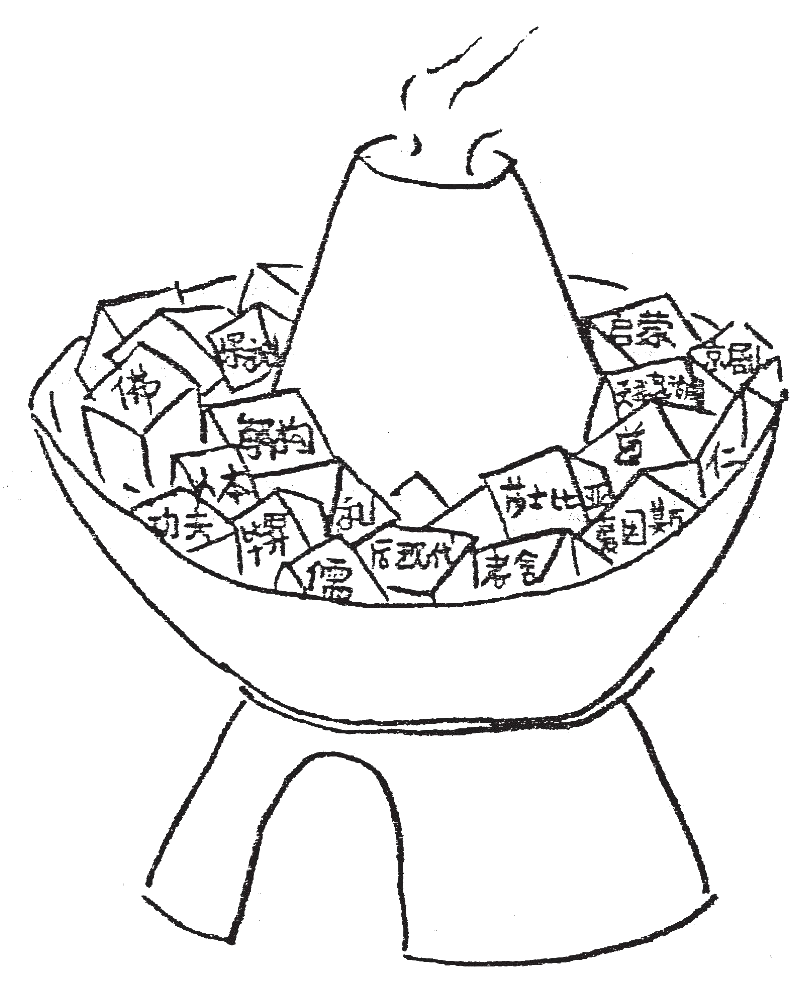
\includegraphics[width=0.36\linewidth]{picture/2010.png}
	\caption*{文化“火锅”,既美味又营养}
\end{figure}

%

\bta{2011}


\section{Use of English}

\noindent
\textbf{Directions:}\\
Read the following text. Choose the best word (s) for each
	numbered blank and mark A, B, C or D on \textbf{ANSWER SHEET 1}. (10 points)



\TiGanSpace

Ancient Greek philosopher Aristotle viewed laughter as ``a bodily
exercise precious to health.'' But \cloze some claims to the
contrary, laughing probably has little influence on physical fitness.
Laughter does \cloze short-term changes in the function of the
heart and its blood vessels, \cloze heart rate and oxygen
consumption. But because hard laughter is difficult to \cloze , a
good laugh is unlikely to have \cloze benefits the way, say,
walking or jogging does.

\cloze , instead of straining muscles to build them, as exercise
does, laughter apparently accomplishes the \cloze. Studies dating
back to the 1930s indicate that laughter \cloze muscles,
decreasing muscle tone for up to 45 minutes after the laugh dies down.

Such bodily reaction might conceivably help \cloze the effects of
psychological stress. Anyway, the act of laughing probably does produce
other types of \cloze feedback that improve an individual's
emotional state. \cloze one classical theory of emotion, our
feelings are partially rooted \cloze physical reactions. It was
argued at the end of the 19\textsuperscript{th} century that humans do
not cry \cloze they are sad but that they become sad when the
tears begin to flow.

Although sadness also \cloze tears, evidence suggests that
emotions can flow \cloze muscular responses. In an experiment
published in 1988, social psychologist Fritz Strack of the University of
Würzburg in Germany asked volunteers to \cloze a pen either with
their teeth -- thereby creating an artificial smile -- or with their
lips, which would produce a(n) \cloze expression. Those forced
to exercise their smiling muscles \cloze more enthusiastically
to funny cartoons than did those whose mouths were contracted in a
frown, \cloze that expressions may influence emotions rather
than just the other way around. \cloze , the physical act of
laughter could improve mood.



\newpage

\begin{enumerate}
	%\renewcommand{\labelenumi}{\arabic{enumi}.}
	% A(\Alph) a(\alph) I(\Roman) i(\roman) 1(\arabic)
	%设定全局标号series=example	%引用全局变量resume=example
	%[topsep=-0.3em,parsep=-0.3em,itemsep=-0.3em,partopsep=-0.3em]
	%可使用leftmargin调整列表环境左边的空白长度 [leftmargin=0em]
	\item


\fourchoices
{among}
{except}
{despite}
{like}




\item


\fourchoices
{reflect}
{demand}
{indicate}
{produce}




\item

\fourchoices
{stabilizing}
{boosting}
{impairing}
{determining}




\item


\fourchoices
{transmit}
{sustain}
{evaluate}
{observe}




\item

\fourchoices
{measurable}
{manageable}
{affordable}
{renewable}




\item


\fourchoices
{In turn}
{In fact}
{In addition}
{In brief}




\item


\fourchoices
{opposite}
{impossible}
{average}
{expected}




\item


\fourchoices
{hardens}
{weakens}
{tightens}
{relaxes}




\item


\fourchoices
{aggravate}
{generate}
{moderate}
{enhance}




\item


\fourchoices
{physical}
{mental}
{subconscious}
{internal}




\item


\fourchoices
{Except for}
{According to}
{Due to}
{As for}




\item


\fourchoices
{with}
{on}
{in}
{at}




\item


\fourchoices
{unless}
{until}
{if}
{because}




\item


\fourchoices
{exhausts}
{follows}
{precedes}
{suppresses}




\item


\fourchoices
{into}
{from}
{towards}
{beyond}




\item

	
\fourchoices
{fetch}
{bite}
{pick}
{hold}




\item

\fourchoices
{disappointed}
{excited}
{joyful}
{indifferent}




\item


\fourchoices
{adapted}
{catered}
{turned}
{reacted}




\item

\fourchoices
{suggesting}
{requiring}
{mentioning}
{supposing}




\item

\fourchoices
{Eventually}
{Consequently}
{Similarly}
{Conversely}

\end{enumerate}


\vfil


\section{Reading Comprehension}


\noindent
\textbf{Part A}\\
\textbf{Directions:}\\
Read the following four texts. Answer the questions below each
	text by choosing A, B, C or
	D. Mark your answers on \textbf{ANSWER SHEET 1}. (40
	points)

\newpage
\subsection{Text 1}


The decision of the New York Philharmonic to hire Alan Gilbert as its
next music director has been the talk of the classical-music world ever
since the sudden announcement of his appointment in 2009. For the most
part, the response has been favorable, to say the least. ``Hooray! At
last!'' wrote Anthony Tommasini, a sober-sided classical-music critic.

One of the reasons why the appointment came as such a surprise, however,
is that Gilbert is comparatively little known. Even Tommasini, who had
advocated Gilbert's appointment in the \emph{Times}, calls him ``an
unpretentious musician with no air of the formidable conductor about
him.'' As a description of the next music director of an orchestra that
has hitherto been led by musicians like Gustav Mahler and Pierre Boulez,
that seems likely to have struck at least some \emph{Times} readers as
faint praise.

For my part, I have no idea whether Gilbert is a great conductor or even
a good one. To be sure, he performs an impressive variety of interesting
compositions, but it is not necessary for me to visit Avery Fisher Hall,
or anywhere else, to hear interesting orchestral music. All I have to do
is to go to my CD shelf, or boot up my computer and download still more
recorded music from iTunes.

Devoted concertgoers who reply that recordings are no substitute for
live performance are missing the point. For the time, attention, and
money of the art-loving public, classical instrumentalists must compete
not only with opera houses, dance troupes, theater companies, and
museums, but also with the recorded performances of the great classical
musicians of the 20th century. These recordings are
cheap, available everywhere, and very often much higher in artistic
quality than today's live performances; moreover, they can be
``consumed'' at a time and place of the listener's choosing. The
widespread availability of such recordings has thus brought about a
crisis in the institution of the traditional classical concert.

One possible response is for classical performers to program attractive
new music that is not yet available on record. Gilbert's own interest in
new music has been widely noted: Alex Ross, a classical-music critic,
has described him as a man who is capable of turning the Philharmonic
into ``a markedly different, more vibrant organization.'' But what will
be the nature of that difference? Merely expanding the orchestra's
repertoire will not be enough. If Gilbert and the Philharmonic are to
succeed, they must first change the relationship between America's
oldest orchestra and the new audience it hopes to attract.


\begin{enumerate}[resume]
	%\renewcommand{\labelenumi}{\arabic{enumi}.}
	% A(\Alph) a(\alph) I(\Roman) i(\roman) 1(\arabic)
	%设定全局标号series=example	%引用全局变量resume=example
	%[topsep=-0.3em,parsep=-0.3em,itemsep=-0.3em,partopsep=-0.3em]
	%可使用leftmargin调整列表环境左边的空白长度 [leftmargin=0em]
	\item
 We learn from Paragraph 1 that Gilbert's appointment has \lineread.


\fourchoices
{incurred criticism}
{raised suspicion}
{received acclaim}
{aroused curiosity}



\item
Tommasini regards Gilbert as an artist who is \lineread.


\fourchoices
{influential}
{modest}
{respectable}
{talented}




\item
The author believes that the devoted concertgoers \lineread.


\fourchoices
{ignore the expenses of live performances.}
{reject most kinds of recorded performances.}
{exaggerate the variety of live performances.}
{overestimate the value of live performances.}


\item
 According to the text, which of the following is
true of recordings?


\fourchoices
{They are often inferior to live concerts in quality.}
{They are easily accessible to the general public.}
{They help improve the quality of music.}
{They have only covered masterpieces.}



\item
Regarding Gilbert's role in revitalizing the
Philharmonic, the author feels \lineread.


\fourchoices
{doubtful}
{enthusiastic}
{confident}
{puzzled}




\end{enumerate}



\newpage
\subsection{Text 2}


When Liam McGee departed as president of Bank of America in August, his
explanation was surprisingly straight up. Rather than cloaking his exit
in the usual vague excuses, he came right out and said he was leaving
``to pursue my goal of running a company.'' Broadcasting his ambition
was ``very much my decision,'' McGee says. Within two weeks, he was
talking for the first time with the board of Hartford Financial Services
Group, which named him CEO and chairman on September 29.

McGee says leaving without a position lined up gave him time to reflect
on what kind of company he wanted to run. It also sent a clear message
to the outside world about his aspirations. And McGee isn't alone. In
recent weeks the No. 2 executives at Avon and American Express quit with
the explanation that they were looking for a CEO post. As boards
scrutinize succession plans in response to shareholder pressure,
executives who don't get the nod also may wish to move on. A turbulent
business environment also has senior managers cautious of letting vague
pronouncements cloud their reputations.

As the first signs of recovery begin to take hold, deputy chiefs may be
more willing to make the jump without a net. In the third quarter, CEO
turnover was down 23\% from a year ago as nervous boards stuck with the
leaders they had, according to Liberum Research. As the economy picks
up, opportunities will abound for aspiring leaders.

The decision to quit a senior position to look for a better one is
unconventional. For years executives and headhunters have adhered to the
rule that the most attractive CEO candidates are the ones who must
be \uline{poached}. Says Korn/Ferry senior partner Dennis Carey: ``I
can't think of a single search I've done where a board has not
instructed me to look at sitting CEOs first.''

Those who jumped without a job haven't always landed in top positions
quickly. Ellen Marram quit as chief of Tropicana a decade ago, saying
she wanted to be a CEO. It was a year before she became head of a tiny
Internet-based commodities exchange. Robert Willumstad left Citigroup in
2005 with ambitions to be a CEO. He finally took that post at a major
financial institution three years later.

Many recruiters say the old disgrace is fading for top performers. The
financial crisis has made it more acceptable to be between jobs or to
leave a bad one. ``The traditional rule was it's safer to stay where you
are, but that's been fundamentally inverted,'' says one headhunter.
``The people who've been hurt the worst are those who've stayed too
long.''


\begin{enumerate}[resume]
	%\renewcommand{\labelenumi}{\arabic{enumi}.}
	% A(\Alph) a(\alph) I(\Roman) i(\roman) 1(\arabic)
	%设定全局标号series=example	%引用全局变量resume=example
	%[topsep=-0.3em,parsep=-0.3em,itemsep=-0.3em,partopsep=-0.3em]
	%可使用leftmargin调整列表环境左边的空白长度 [leftmargin=0em]
	\item
 When McGee announced his departure, his manner can
best be described as being \lineread.


\fourchoices
{arrogant}
{frank}
{self-centered}
{impulsive}



\item
According to Paragraph 2, senior executives'
quitting may be spurred by \lineread.


\fourchoices
{their expectation of better financial status}
{their need to reflect on their private life}
{their strained relations with the boards}
{their pursuit of new career goals}



\item
The word ``poached'' (Line 3, Paragraph 4) most
probably means\lineread.


\fourchoices
{approved of}
{attended to}
{hunted for}
{guarded against}


\item
 It can be inferred from the last paragraph that \lineread.

\fourchoices
{top performers used to cling to their posts}
{loyalty of top performers is getting out-dated}
{top performers care more about reputations}
{it's safer to stick to the traditional rules}


\item
Which of the following is the best title for the
text?


\fourchoices
{CEOs: Where to Go?}
{CEOs: All the Way Up?}
{Top Managers Jump without a Net}
{The Only Way Out for Top Performers}


\end{enumerate}


\newpage
\subsection{Text 3}


The rough guide to marketing success used to be that you got what you
paid for. No longer. While traditional ``paid'' media---such as
television commercials and print advertisements---still play a major
role, companies today can exploit many alternative forms of media.
Consumers passionate about a product may create ``earned'' media by
willingly promoting it to friends, and a company may leverage ``owned''
media by sending e-mail alerts about products and sales to customers
registered with its Web site. The way consumers now approach the process
of making purchase decisions means that marketing's impact stems from a
broad range of factors beyond conventional paid media.

Paid and owned media are controlled by marketers promoting their own
products. For earned media, such marketers act as the initiator for
users' responses. But in some cases, one marketer's owned media become
another marketer's paid media---for instance, when an e-commerce
retailer sells ad space on its Web site. We define such sold media as
owned media whose traffic is so strong that other organizations place
their content or e-commerce engines within that environment. This trend,
which we believe is still in its infancy, effectively began with
retailers and travel providers such as airlines and hotels and will no
doubt go further. Johnson \& Johnson, for example, has created
BabyCenter, a stand-alone media property that promotes complementary and
even competitive products. Besides generating income, the presence of
other marketers makes the site seem objective, gives companies
opportunities to learn valuable information about the appeal of other
companies' marketing, and may help expand user traffic for all companies
concerned.

The same dramatic technological changes that have provided marketers
with more (and more diverse) communications choices have also increased
the risk that passionate consumers will voice their opinions in quicker,
more visible, and much more damaging ways. Such hijacked media are the
opposite of earned media: an asset or campaign becomes hostage to
consumers, other stakeholders, or activists who make negative
allegations about a brand or product. Members of social networks, for
instance, are learning that they can hijack media to apply pressure on
the businesses that originally created them.

If that happens, passionate consumers would try to persuade others to
boycott products, putting the reputation of the target company at risk.
In such a case, the company's response may not be sufficiently quick or
thoughtful, and the learning curve has been steep. Toyota Motor, for
example, alleviated some of the damage from its recall crisis earlier
this year with a relatively quick and well-orchestrated social-media
response campaign, which included efforts to engage with consumers
directly on sites such as Twitter and the social-news site Digg.


\begin{enumerate}[resume]
	%\renewcommand{\labelenumi}{\arabic{enumi}.}
	% A(\Alph) a(\alph) I(\Roman) i(\roman) 1(\arabic)
	%设定全局标号series=example	%引用全局变量resume=example
	%[topsep=-0.3em,parsep=-0.3em,itemsep=-0.3em,partopsep=-0.3em]
	%可使用leftmargin调整列表环境左边的空白长度 [leftmargin=0em]
	\item
 Consumers may create ``earned'' media when they are \lineread.


\fourchoices
{obsessed with online shopping at certain Web sites}
{inspired by product-promoting e-mails sent to them}
{eager to help their friends promote quality products}
{enthusiastic about recommending their favorite products}


\item
 According to Paragraph 2, sold media feature \lineread.


\fourchoices
{a safe business environment}
{random competition}
{strong user traffic}
{flexibility in organization}



\item
The author indicates in Paragraph 3 that earned media \lineread.


\fourchoices
{invite constant conflicts with passionate consumers}
{can be used to produce negative effects in marketing}
{may be responsible for fiercer competition}
{deserve all the negative comments about them}


\item
Toyota Motor's experience is cited as an example of \lineread.


\fourchoices
{responding effectively to hijacked media}
{persuading customers into boycotting products}
{cooperating with supportive consumers}
{taking advantage of hijacked media}


\item
Which of the following is the text mainly about?


\fourchoices
{Alternatives to conventional paid media.}
{Conflict between hijacked and earned media.}
{Dominance of hijacked media.}
{Popularity of owned media.}

\end{enumerate}



\newpage
\subsection{Text 4}


It's no surprise that Jennifer Senior's insightful, provocative magazine
cover story, ``I Love My Children, I Hate My Life,'' is arousing much
chatter---nothing gets people talking like the suggestion that child
rearing is anything less than a completely fulfilling, life-enriching
experience. Rather than concluding that children make parents either
happy or miserable, Senior suggests we need to redefine happiness:
instead of thinking of it as something that can be measured by
moment-to-moment joy, we should consider being happy as a past-tense
condition. Even though the day-to-day experience of raising kids can be
soul-crushingly hard, Senior writes that ``the very things that in the
moment dampen our moods can later be sources of intense gratification
and delight.''

The magazine cover showing an attractive mother holding a cute baby is
hardly the only Madonna-and-child image on newsstands this week. There
are also stories about newly adoptive---and newly single---mom Sandra
Bullock, as well as the usual ``Jennifer Aniston is pregnant'' news.
Practically every week features at least one celebrity mom, or
mom-to-be, smiling on the newsstands.

In a society that so persistently celebrates procreation, is it any
wonder that admitting you regret having children is equivalent to
admitting you support kitten-killing? It doesn't seem quite fair, then,
to compare the regrets of parents to the regrets of the childless.
Unhappy parents rarely are provoked to wonder if they shouldn't have had
kids, but unhappy childless folks are bothered with the message that
children are the single most important thing in the world: obviously
their misery must be a direct result of the gaping baby-size holes in
their lives.

Of course, the image of parenthood that celebrity magazines
like \emph{Us Weekly} and \emph{People} present is hugely unrealistic,
especially when the parents are single mothers like Bullock. According
to several studies concluding that parents are less happy than childless
couples, single parents are the least happy of all. No shock there,
considering how much work it is to raise a kid without a partner to lean
on; yet to hear Sandra and Britney tell it, raising a kid on their
``own'' (read: with round-the-clock help) is a piece of cake.

It's hard to imagine that many people are dumb enough to want children
just because Reese and Angelina make it look so glamorous: most adults
understand that a baby is not a haircut. But it's interesting to wonder
if the images we see every week of stress-free, happiness-enhancing
parenthood aren't in some small, subconscious way contributing to our
own dissatisfactions with the actual experience, in the same way that a
small part of us hoped getting ``the Rachel'' might make us look just a
little bit like Jennifer Aniston.

\begin{enumerate}[resume]
	%\renewcommand{\labelenumi}{\arabic{enumi}.}
	% A(\Alph) a(\alph) I(\Roman) i(\roman) 1(\arabic)
	%设定全局标号series=example	%引用全局变量resume=example
	%[topsep=-0.3em,parsep=-0.3em,itemsep=-0.3em,partopsep=-0.3em]
	%可使用leftmargin调整列表环境左边的空白长度 [leftmargin=0em]
	\item
 Jennifer Senior suggests in her article that
raising a child can bring \lineread.


\fourchoices
{temporary delight}
{enjoyment in progress}
{happiness in retrospect}
{lasting reward}



\item 
We learn from Paragraph 2 that \lineread.


\fourchoices
{celebrity moms are a permanent source for gossip}
{single mothers with babies deserve greater attention}
{news about pregnant celebrities is entertaining}
{having children is highly valued by the public}




\item
 It is suggested in Paragraph 3 that childless folks \lineread.


\fourchoices
{are constantly exposed to criticism}
{are largely ignored by the media}
{fail to fulfill their social responsibilities}
{are less likely to be satisfied with their life}




\item
According to Paragraph 4, the message conveyed by celebrity
magazines is \lineread.


\fourchoices
{soothing}
{ambiguous}
{compensatory}
{misleading}




\item
Which of the following can be inferred from the last
paragraph?


\fourchoices
{Having children contributes little to the glamour of celebrity moms.}
{Celebrity moms have influenced our attitude towards child rearing.}
{Having children intensifies our dissatisfaction with life.}
{We sometimes neglect the happiness from child rearing.}



	
\end{enumerate}


\newpage
\noindent
\textbf{Part B}\\
\textbf{Directions:}\\
The following paragraphs are given in a wrong order. For
	questions 41-45, you are required to reorganize these paragraphs into a
	coherent text by choosing from the list A-G and filling them into the
	numbered boxes. Paragraphs E and G have been correctly placed. Mark your
	answers on \textbf{ANSWER SHEET 1}. (10 points)


\begin{listmatch}
	%\renewcommand{\labelenumi}{\arabic{enumi}.}
	% A(\Alph) a(\alph) I(\Roman) i(\roman) 1(\arabic)
	%设定全局标号series=example	%引用全局变量resume=example
	%[topsep=-0.3em,parsep=-0.3em,itemsep=-0.3em,partopsep=-0.3em]
	%可使用leftmargin调整列表环境左边的空白长度 [leftmargin=0em]
	\item
No disciplines have seized on professionalism with as much
enthusiasm as the humanities. You can, Mr Menand points out, become a
lawyer in three years and a medical doctor in four. But the regular time
it takes to get a doctoral degree in the humanities is nine years. Not
surprisingly, up to half of all doctoral students in English drop out
before getting their degrees.


\item 
His concern is mainly with the humanities: literature,
languages, philosophy and so on. These are disciplines that are going
out of style: 22\% of American college graduates now major in business
compared with only 2\% in history and 4\% in English. However, many
leading American universities want their undergraduates to have a
grounding in the basic canon of ideas that every educated person should
possess. But most find it difficult to agree on what a ``general
education'' should look like. At Harvard, Mr Menand notes, ``the great
books are read because they have been read'' -- they form a sort of
social glue.


\item 
Equally unsurprisingly, only about half end up with
professorships for which they entered graduate school. There are simply
too few posts. This is partly because universities continue to produce
ever more PhDs. But fewer students want to study humanities subjects:
English departments awarded more bachelor's degrees in 1970-71 than they
did 20 years later. Fewer students require fewer teachers. So, at the
end of a decade of thesis-writing, many humanities students leave the
profession to do something for which they have not been trained.


\item 
One reason why it is hard to design and teach such courses is
that they cut across the insistence by top American universities that
liberal-arts education and professional education should be kept
separate, taught in different schools. Many students experience both
varieties. Although more than half of Harvard undergraduates end up in
law, medicine or business, future doctors and lawyers must study a
non-specialist liberal-arts degree before embarking on a professional
qualification.


\item 
Besides professionalising the professions by this separation,
top American universities have professionalised the professor. The
growth in public money for academic research has speeded the process:
federal research grants rose fourfold between 1960 and 1990, but faculty
teaching hours fell by half as research took its toll. Professionalism
has turned the acquisition of a doctoral degree into a prerequisite for
a successful academic career: as late as 1969 a third of American
professors did not possess one. But the key idea behind
professionalisation, argues Mr Menand, is that ``the knowledge and
skills needed for a particular specialisation are transmissible but not
transferable.'' So disciplines acquire a monopoly not just over the
production of knowledge, but also over the production of the producers
of knowledge.


\item 
The key to reforming higher education, concludes Mr Menand, is
to alter the way in which ``the producers of knowledge are produced.''
Otherwise, academics will continue to think dangerously alike,
increasingly detached from the societies which they study, investigate
and criticise. ``Academic inquiry, at least in some fields, may need to
become less exclusionary and more holistic.'' Yet quite how that
happens, Mr Menand does not say.


\item 
The subtle and intelligent little book \emph{The Marketplace of
	Ideas: Reform and Resistance in the American University} should be read
by every student thinking of applying to take a doctoral degree. They
may then decide to go elsewhere. For something curious has been
happening in American universities, and Louis Menand, a professor of
English at Harvard University, captured it skillfully.

\end{listmatch}


\[ 
\begin{tabular}{|c|}
	\hline
	G \\
	\hline
\end{tabular}
\rightarrow
\begin{tabular}{|c|c|}
	\hline
	41. &  \hspace{1.5em} \\
	\hline
\end{tabular}
\rightarrow
\begin{tabular}{|c|c|}
	\hline
	42. &  \hspace{1.5em} \\
	\hline
\end{tabular}
\rightarrow
\begin{tabular}{|c|}
	\hline
	E \\
	\hline
\end{tabular}
\rightarrow
\begin{tabular}{|c|c|}
	\hline
	43. &  \hspace{1.5em} \\
	\hline
\end{tabular}
\rightarrow
\begin{tabular}{|c|c|}
	\hline
	44. &  \hspace{1.5em} \\
	\hline
\end{tabular}
\rightarrow
\begin{tabular}{|c|c|}
	\hline
	45. &  \hspace{1.5em} \\
	\hline
\end{tabular}
\]


\phantom{ \linefill \linefill \linefill \linefill \linefill}



\newpage
\noindent
\textbf{Part C}\\
\textbf{Directions:}\\
Read the following text carefully and then translate the
	underlined segments into Chinese. Your translation should be written
	clearly on \textbf{ANSWER SHEET 2}. (10 points)

\TiGanSpace


With its theme that ``Mind is the master weaver,'' creating our inner
character and outer circumstances, the book \emph{As a Man Thinketh} by
James Allen is an in-depth exploration of the central idea of self-help
writing.

\transnum \uline{Allen's contribution was to take an assumption we all
	share -- that because we are not robots we therefore control our
	thoughts -- and reveal its erroneous nature.} Because most of us believe
that mind is separate from matter, we think that thoughts can be hidden
and made powerless; this allows us to think one way and act another.
However, Allen believed that the unconscious mind generates as much
action as the conscious mind, and \transnum \uline{while we may be able to
	sustain the illusion of control through the conscious mind alone, in
	reality we are continually faced with a question: ``Why cannot I make
	myself do this or achieve that?\,''}

Since desire and will are damaged by the presence of thoughts that do
not accord with desire, Allen concluded: ``We do not attract what we
want, but what we are.'' Achievement happens because you as a person
embody the external achievement; you don't ``get'' success but become it.
There is no gap between mind and matter.

Part of the fame of Allen's book is its contention that ``Circumstances
do not make a person, they reveal him.'' \transnum \uline{This seems a
	justification for neglect of those in need, and a rationalization of
	exploitation, of the superiority of those at the top and the inferiority
	of those at the bottom.}

This, however, would be a knee-jerk reaction to a subtle argument. Each
set of circumstances, however bad, offers a unique opportunity for
growth. If circumstances always determined the life and prospects of
people, then humanity would never have progressed. In fact,
\transnum \uline{circumstances seem to be designed to bring out the best
	in us, and if we feel that we have been ``wronged'' then we are unlikely
	to begin a conscious effort to escape from our situation.} Nevertheless,
as any biographer knows, a person's early life and its conditions are
often the greatest gift to an individual.

The sobering aspect of Allen's book is that we have no one else to blame
for our present condition except ourselves. \transnum \uline{The upside
	is the possibilities contained in knowing that everything is up to us;
	where before we were experts in the array of limitations, now we become
	authorities of what is possible.}



\newpage

\section{Writing}


\noindent
\textbf{Part A}\\
\textbf{51. Directions:}

Write a letter to a friend of yours to
\begin{listwrite}
	%\renewcommand{\labelenumi}{\arabic{enumi}.}
	% A(\Alph) a(\alph) I(\Roman) i(\roman) 1(\arabic)
	%设定全局标号series=example	%引用全局变量resume=example
	%[topsep=-0.3em,parsep=-0.3em,itemsep=-0.3em,partopsep=-0.3em]
	%可使用leftmargin调整列表环境左边的空白长度 [leftmargin=0em]
	\item
recommend one of your favorite movies and

\item 
 give reasons for your recommendation.
\end{listwrite}

You should write about 100 words on ANSWER SHEET 2.

\textbf{Do not} sign your own name at the end of the letter. Use ``Li
Ming'' instead.

\textbf{Do not} write the address. (10 points)



\vspace{2em}

\noindent
\textbf{Part B}\\
\textbf{52. Directions:}

Write an essay of 160-200 words based on the following drawing. In your
essay, you should
\begin{listwrite}
	%\renewcommand{\labelenumi}{\arabic{enumi}.}
	% A(\Alph) a(\alph) I(\Roman) i(\roman) 1(\arabic)
	%设定全局标号series=example	%引用全局变量resume=example
	%[topsep=-0.3em,parsep=-0.3em,itemsep=-0.3em,partopsep=-0.3em]
	%可使用leftmargin调整列表环境左边的空白长度 [leftmargin=0em]
	\item
 describe the drawing briefly,

\item 
 explain its intended meaning, and

\item 
 give your comments.
\end{listwrite}

You should write neatly on ANSWER SHEET 2. (20 points)

\begin{figure}[h!]
	\centering
	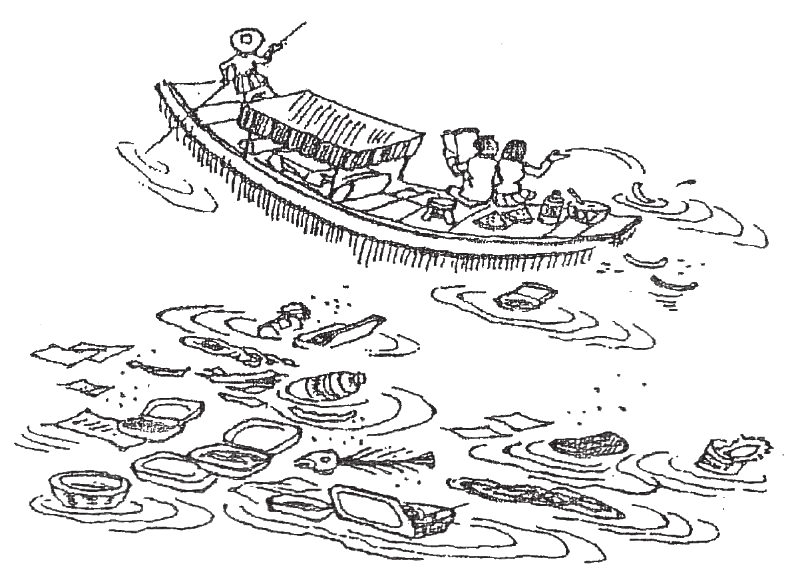
\includegraphics[width=0.54\linewidth]{picture/2011.png}
	\caption*{旅程之“余”}
\end{figure}

\checkpagenumber%

\bta{2012}



\section{Use of English}

\noindent
\textbf{Directions:}\\
Read the following text. Choose the best word (s) for each
	numbered blank and mark A, B, C or D on \textbf{ANSWER SHEET 1}.  (10 points)



\TiGanSpace


The ethical judgments of the Supreme Court justices have become an
important issue recently. The court cannot \cloze its
legitimacy as guardian of the rule of law \cloze justices
behave like politicians. Yet, in several instances, justices acted in
ways that \cloze the court's reputation for being independent
and impartial.

Justice Antonin Scalia, for example, appeared at political events. That
kind of activity makes it less likely that the court's decisions will
be \cloze as impartial judgments. Part of the problem is that
the justices are not \cloze by an ethics code. At the very
least, the court should make itself \cloze to the code of
conduct that \cloze to the rest of the federal judiciary.

This and other similar cases \cloze the question of whether
there is still a \cloze between the court and politics.

The framers of the Constitution envisioned law \cloze having
authority apart from politics. They gave justices permanent positions
\cloze they would be free to \cloze those in power
and have no need to \cloze political support. Our legal system
was designed to set law apart from politics precisely because they are
so closely \cloze.

Constitutional law is political because it results from choices rooted
in fundamental social \cloze like liberty and property. When
the court deals with social policy decisions, the law it \cloze
is inescapably political---which is why decisions split along
ideological lines are so easily \cloze as unjust.

The justices must \cloze doubts about the court's legitimacy
by making themselves \cloze to the code of conduct. That would
make their rulings more likely to be seen as separate from politics and,
\cloze , convincing as law.


\newpage

\begin{enumerate}
	%\renewcommand{\labelenumi}{\arabic{enumi}.}
	% A(\Alph) a(\alph) I(\Roman) i(\roman) 1(\arabic)
	%设定全局标号series=example	%引用全局变量resume=example
	%[topsep=-0.3em,parsep=-0.3em,itemsep=-0.3em,partopsep=-0.3em]
	%可使用leftmargin调整列表环境左边的空白长度 [leftmargin=0em]
	\item


\fourchoices
{emphasize}
{maintain}
{modify}
{recognize}




\item


\fourchoices
{when}
{lest}
{before}
{unless}




\item


\fourchoices
{restored}
{weakened}
{established}
{eliminated}




\item


\fourchoices
{challenged}
{compromised}
{suspected}
{accepted}




\item


\fourchoices
{advanced}
{caught}
{bound}
{founded}




\item


\fourchoices
{resistant}
{subject}
{immune}
{prone}




\item


\fourchoices
{resorts}
{sticks}
{leads}
{applies}




\item


\fourchoices
{evade}
{raise}
{deny}
{settle}




\item


\fourchoices
{line}
{barrier}
{similarity}
{conflict}




\item


\fourchoices
{by}
{as}
{through}
{towards}




\item


\fourchoices
{so}
{since}
{provided}
{though}




\item


\fourchoices
{serve}
{satisfy}
{upset}
{replace}




\item


\fourchoices
{confirm}
{express}
{cultivate}
{offer}




\item


\fourchoices
{guarded}
{followed}
{studied}
{tied}




\item


\fourchoices
{concepts}
{theories}
{divisions}
{conventions}




\item


\fourchoices
{excludes}
{questions}
{shapes}
{controls}




\item


\fourchoices
{dismissed}
{released}
{ranked}
{distorted}




\item


\fourchoices
{suppress}
{exploit}
{address}
{ignore}




\item


\fourchoices
{accessible}
{amiable}
{agreeable}
{accountable}




\item


\fourchoices
{by all means}
{at all costs}
{in a word}
{as a result}


\end{enumerate}


\vfil

\section{Reading Comprehension}


\noindent
\textbf{Part A}\\
\textbf{Directions:}\\
Read the following four texts. Answer the questions below each
	text by choosing A, B, C or
	D. Mark your answers on \textbf{ANSWER SHEET 1}. (40
	points)

\newpage
\subsection{Text 1}


Come on---Everybody's doing it. That whispered message, half
invitation and half forcing, is what most of us think of when we hear
the words \emph{peer pressure.} It usually leads to no good---drinking, drugs and casual sex.
But in her new book \emph{Join the Club}, Tina Rosenberg contends that peer pressure can also be a positive
force through what she calls the social cure, in which organizations and
officials use the power of group dynamics to help individuals improve
their lives and possibly the world.

Rosenberg, the recipient of a Pulitzer Prize, offers a host of examples
of the social cure in action: In South Carolina, a state-sponsored
antismoking program called Rage Against the Haze sets out to make
cigarettes uncool. In South Africa, an HIV-prevention initiative known
as loveLife recruits young people to promote safe sex among their peers.

The idea seems promising, and Rosenberg is a perceptive observer. Her
critique of the lameness of many public-health campaigns is
spot-on: they fail to mobilize peer pressure for healthy habits, and
they demonstrate a seriously flawed understanding of psychology. ``Dare
to be different, please don't smoke!'' pleads one billboard campaign
aimed at reducing smoking among teenagers---teenagers, who desire
nothing more than fitting in. Rosenberg argues convincingly that
public-health advocates ought to take a page from advertisers, so
skilled at applying peer pressure.

But on the general effectiveness of the social cure, Rosenberg is less
persuasive. \emph{Join the Club} is filled with too much irrelevant
detail and not enough exploration of the social and biological factors
that make peer pressure so powerful. The most glaring flaw of the social
cure as it's presented here is that it doesn't work very well for very
long. Rage Against the Haze failed once state funding was cut. Evidence
that the loveLife program produces lasting changes is limited and mixed.

There's no doubt that our peer groups exert enormous influence on our
behavior. An emerging body of research shows that positive health habits---as well as negative ones---spread through networks of friends via
social communication. This is a subtle form of peer pressure: we
unconsciously imitate the behavior we see every day.

Far less certain, however, is how successfully experts and bureaucrats
can select our peer groups and steer their activities in virtuous
directions. It's like the teacher who breaks up the troublemakers in the
back row by pairing them with better-behaved classmates. The tactic
never really works. And that's the problem with a social cure engineered
from the outside: in the real world, as in school, we insist on choosing
our own friends.

\begin{enumerate}[resume]
	%\renewcommand{\labelenumi}{\arabic{enumi}.}
	% A(\Alph) a(\alph) I(\Roman) i(\roman) 1(\arabic)
	%设定全局标号series=example	%引用全局变量resume=example
	%[topsep=-0.3em,parsep=-0.3em,itemsep=-0.3em,partopsep=-0.3em]
	%可使用leftmargin调整列表环境左边的空白长度 [leftmargin=0em]
	\item
According to the first
paragraph, peer pressure often emerges as \lineread.


\fourchoices
{a supplement to the social cure}
{a stimulus to group dynamics}
{an obstacle to social progress}
{a cause of undesirable behaviors}


\item
Rosenberg holds that public advocates should \lineread.


\fourchoices
{recruit professional advertisers}
{learn from advertisers' experience}
{stay away from commercial advertisers}
{recognize the limitations of advertisements}



\item
 In the author's view, Rosenberg's book fails to \lineread.


\fourchoices
{adequately probe social and biological factors}
{effectively evade the flaws of the social cure}
{illustrate the functions of state funding}
{produce a long-lasting social effect}


\item
Paragraph 5 shows that our imitation of behaviors \lineread.


\fourchoices
{is harmful to our networks of friends}
{will mislead behavioral studies}
{occurs without our realizing it}
{can produce negative health habits}


\item
 The author suggests in the last paragraph that the effect
ofpeer pressure is \lineread.



\fourchoices
{harmful}
{desirable}
{profound}
{questionable}

\end{enumerate}



\newpage
\subsection{Text 2}


A deal is a deal---except, apparently, when Entergy is involved. The
company, a major energy supplier in New England, provoked justified
outrage in Vermont last week when it announced it was
\uline{reneging on} a longstanding commitment to abide by the strict
nuclear regulations.

Instead, the company has done precisely what it had long promised it
would not: challenge the constitutionality of Vermont's rules in the
federal court, as part of a desperate effort to keep its Vermont Yankee
nuclear power plant running. It's a stunning move.

The conflict has been surfacing since 2002, when the corporation bought
Vermont's only nuclear power plant, an aging reactor in Vernon. As a
condition of receiving state approval for the sale, the company agreed
to seek permission from state regulators to operate past 2012. In 2006,
the state went a step further, requiring that any extension of the
plant's license be subject to Vermont legislature's approval. Then, too,
the company went along.

Either Entergy never really intended to live by those commitments, or it
simply didn't foresee what would happen next. A string of accidents,
including the partial collapse of a cooling tower in 2007 and the
discovery of an underground pipe system leakage, raised serious
questions about both Vermont Yankee's safety and Entergy's management---especially after the company made misleading statements about the
pipe. Enraged by Entergy's behavior, the Vermont Senate voted 26 to 4
last year against allowing an extension.

Now the company is suddenly claiming that the 2002 agreement is invalid
because of the 2006 legislation, and that only the federal government
has regulatory power over nuclear issues. The legal issues in the case
are obscure: whereas the Supreme Court has ruled that states do have
some regulatory authority over nuclear power, legal scholars say that
Vermont case will offer a precedent-setting test of how far those powers
extend. Certainly, there are valid concerns about the patchwork
regulations that could result if every state sets its own rules. But had
Entergy kept its word, that debate would be beside the point.

The company seems to have concluded that its reputation in Vermont is
already so damaged that it has nothing left to lose by going to war with
the state. But there should be consequences. Permission to run a nuclear
plant is a public trust. Entergy runs 11 other reactors in the United
States, including Pilgrim Nuclear station in Plymouth. Pledging to run
Pilgrim safely, the company has applied for federal permission to keep
it open for another 20 years. But as the Nuclear Regulatory Commission
(NRC) reviews the company's application, it should keep it mind what
promises from Entergy are worth.

\begin{enumerate}[resume]
	%\renewcommand{\labelenumi}{\arabic{enumi}.}
	% A(\Alph) a(\alph) I(\Roman) i(\roman) 1(\arabic)
	%设定全局标号series=example	%引用全局变量resume=example
	%[topsep=-0.3em,parsep=-0.3em,itemsep=-0.3em,partopsep=-0.3em]
	%可使用leftmargin调整列表环境左边的空白长度 [leftmargin=0em]
	\item
The phrase ``reneging on'' (Line 3. para. 1) is closest in
meaning to \lineread.


\fourchoices
{condemning}
{reaffirming}
{dishonoring}
{securing}



\item
By entering into the 2002 agreement, Entergy intended to \lineread.


\fourchoices
{obtain protection from Vermont regulators}
{seek favor from the federal legislature}
{acquire an extension of its business license}
{get permission to purchase a power plant}


\item
According to Paragraph 4, Entergy seems to have problems
with its \lineread.


\fourchoices
{managerial practices}
{technical innovativeness}
{financial goals}
{business vision}



\item
 In the author's view, the Vermont case will test \lineread.


\fourchoices
{Entergy's capacity to fulfill all its promises}
{the mature of states' patchwork regulations}
{the federal authority over nuclear issues}
{the limits of states' power over nuclear issues}



\item
It can be inferred from the last paragraph that \lineread.


\fourchoices
{Entergy's business elsewhere might be affected}
{the authority of the NRC will be defied}
{Entergy will withdraw its Plymouth application}
{Vermont's reputation might be damaged}

	
\end{enumerate}



\newpage
\subsection{Text 3}


In the idealized version of how science is done, facts about the world
are waiting to be observed and collected by objective researchers who
use the scientific method to carry out their work. But in the everyday
practice of science, discovery frequently follows an ambiguous and
complicated route. We aim to be objective, but we cannot escape the
context of our unique life experiences. Prior knowledge and interests
influence what we experience, what we think our experiences mean, and
the subsequent actions we take. Opportunities for misinterpretation,
error, and self-deception abound.

Consequently, discovery claims should be thought of as protoscience.
Similar to newly staked mining claims, they are full of potential. But
it takes collective scrutiny and acceptance to transform a discovery
claim into a mature discovery. This is the credibility process, through
which the individual researcher's \emph{me}, \emph{here}, \emph{now} becomes the community's
\emph{anyone}, \emph{anywhere}, \emph{anytime}. Objective knowledge is the goal, not the
starting point.

Once a discovery claim becomes public, the discoverer receives
intellectual credit. But, unlike with mining claims, the community takes
control of what happens next. Within the complex social structure of the
scientific community, researchers make discoveries; editors and
reviewers act as gatekeepers by controlling the publication process;
other scientists use the new finding to suit their own purposes; and
finally, the public (including other scientists) receives the new
discovery and possibly accompanying technology. As a discovery claim
works its way through the community, the interaction and confrontation
between shared and competing beliefs about the science and the
technology involved transforms an individual's discovery claim into the
community's credible discovery.

Two paradoxes exist throughout this credibility process. First,
scientific work tends to focus on some aspect of prevailing knowledge
that is viewed as incomplete or incorrect. Little reward accompanies
duplication and confirmation of what is already known and believed. The
goal is \emph{new-search}, not \emph{re-search.} Not surprisingly, newly
published discovery claims and credible discoveries that appear to be
important and convincing will always be open to challenge and potential
modification or refutation by future researchers. Second, novelty itself
frequently provokes disbelief. Nobel Laureate and physiologist Albert
Szent-Györgyi once described discovery as ``seeing what everybody has
seen and thinking what nobody has thought.'' But thinking what nobody
else has thought and telling others what they have missed may not change
their views. Sometimes years are required for truly novel discovery
claims to be accepted and appreciated.

In the end, credibility ``happens'' to a discovery claim---a process
that corresponds to what philosopher Annette Baier has described as
the \emph{commons of the mind}. ``We reason together, challenge, revise, and
complete each other's reasoning and each other's conceptions of
reason.''

\begin{enumerate}[resume]
	%\renewcommand{\labelenumi}{\arabic{enumi}.}
	% A(\Alph) a(\alph) I(\Roman) i(\roman) 1(\arabic)
	%设定全局标号series=example	%引用全局变量resume=example
	%[topsep=-0.3em,parsep=-0.3em,itemsep=-0.3em,partopsep=-0.3em]
	%可使用leftmargin调整列表环境左边的空白长度 [leftmargin=0em]
	\item
According to the first paragraph, the process of discovery
is characterized by its \lineread.


\fourchoices
{uncertainty and complexity}
{misconception and deceptiveness}
{logicality and objectivity}
{systematicness and regularity}


\item
It can be inferred from Paragraph 2 that credibility process
requires \lineread.


\fourchoices
{strict inspection}
{shared efforts}
{individual wisdom}
{persistent innovation}



\item
Paragraph 3 shows that a discovery claim becomes credible
after it \lineread.


\fourchoices
{has attracted the attention of the general public}
{has been examined by the scientific community}
{has received recognition from editors and reviewers}
{has been frequently quoted by peer scientists}


\item
Albert Szent-Györgyi would most likely agree that \lineread.


\fourchoices
{scientific claims will survive challenges}
{discoveries today inspire future research}
{efforts to make discoveries are justified}
{scientific work calls for a critical mind}


\item
Which of the following would be the best title of the text?


\fourchoices
{Novelty as an Engine of Scientific Development}
{Collective Scrutiny in Scientific Discovery}
{Evolution of Credibility in Doing Science}
{Challenge to Credibility at the Gate to Science}

\end{enumerate}


\newpage
\subsection{Text 4}


If the trade unionist Jimmy Hoffa were alive today, he would probably
represent civil servants. When Hoffa's Teamsters were in their prime in
1960, only one in ten American government workers belonged to a union;
now 36\% do. In 2009 the number of unionists in America's public sector
passed that of their fellow members in the private sector. In Britain,
more than half of public-sector workers but only about 15\% of
private-sector ones are unionized.

There are three reasons for the public-sector unions' thriving. First,
they can shut things down without suffering much in the way of
consequences. Second, they are mostly bright and well-educated. A
quarter of America's public-sector workers have a university degree.
Third, they now dominate left--of--centre politics. Some of their ties go
back a long way. Britain's Labor Party, as its name implies, has long
been associated with trade unionism. Its current leader, Ed Miliband,
owes his position to votes from public--sector unions.

At the state level their influence can be even more fearsome. Mark
Baldassare of the Public Policy Institute of California points out that
much of the state's budget is patrolled by unions. The teachers' unions
keep an eye on schools, the CCPOA on prisons and a variety of labor
groups on health care.

In many rich countries average wages in the state sector are higher than
in the private one. But the real gains come in benefits and work
practices. Politicians have repeatedly ``backloaded'' public-sector pay
deals, keeping the pay increases modest but adding to holidays and
especially pensions that are already generous.

Reform has been vigorously opposed, perhaps most egregiously in
education, where charter schools, academies and merit pay all faced
drawn-out battles. Even though there is plenty of evidence that the
quality of the teachers is the most important variable, teachers' unions
have fought against getting rid of bad ones and promoting good ones.

As the cost to everyone else has become clearer, politicians have begun
to clamp down. In Wisconsin the unions have rallied thousands of
supporters against Scott Walker, the hardline Republican governor. But
many within the public sector suffer under the current system, too.

John Donahue at Harvard's Kennedy School points out that the norms of
culture in Western civil services suit those who want to stay put but is
bad for high achievers. The only American public-sector workers who earn
well above \$250, 000 a year are university sports coaches and the
president of the United States. Bankers' fat pay packets have attracted
much criticism, but a public-sector system that does not reward high
achievers may be a much bigger problem for America.

\begin{enumerate}[resume]
	%\renewcommand{\labelenumi}{\arabic{enumi}.}
	% A(\Alph) a(\alph) I(\Roman) i(\roman) 1(\arabic)
	%设定全局标号series=example	%引用全局变量resume=example
	%[topsep=-0.3em,parsep=-0.3em,itemsep=-0.3em,partopsep=-0.3em]
	%可使用leftmargin调整列表环境左边的空白长度 [leftmargin=0em]
	\item
 It can be learned from the first paragraph that \lineread.


\fourchoices
{Teamsters still have a large body of members}
{Jimmy Hoffa used to work as a civil servant}
{unions have enlarged their public-sector membership}
{the government has improved its relationship with unionists}



\item
Which of the following is true of Paragraph 2?


\fourchoices
{Public-sector unions are prudent in taking actions.}
{Education is required for public-sector union membership.}
{Labor Party has long been fighting against public-sector unions.}
{Public-sector unions seldom get in trouble for their actions.}



\item
It can be learned from Paragraph 4 that the income in the
state sector is \lineread.


\fourchoices
{illegally secured}
{indirectly augmented}
{excessively increased}
{fairly adjusted}



\item
The example of the unions in Wisconsin shows that unions \lineread.


\fourchoices
{often run against the current political system}
{can change people's political attitudes}
{may be a barrier to public-sector reforms}
{are dominant in the government}


\item
John Donahue's attitude towards the public-sector system is
one of \lineread.


\fourchoices
{disapproval}
{appreciation}
{tolerance}
{indifference}


	
\end{enumerate}


\newpage
\noindent
\textbf{Part B}\\
\textbf{Directions:}\\
In the following text, some sentences have been removed. For
	Questions 41-45, choose the most suitable one from the list A-G to fit
	into each of the numbered blanks. There are two extra choices, which do
	not fit in any of the blanks. Mark your answers on \textbf{ANSWER SHEET 1}. (10
	points)



\TiGanSpace

Think of those fleeting moments when you look out of an aeroplane window
and realise that you are flying, higher than a bird. Now think of your
laptop, thinner than a brown-paper envelope, or your cellphone in the
palm of your hand. Take a moment or two to wonder at those marvels. You
are the lucky inheritor of a dream come true.

The second half of the 20th century saw a collection of geniuses,
warriors, entrepreneurs and visionaries labour to create a fabulous
machine that could function as a typewriter and printing press, studio
and theatre, paintbrush and gallery, piano and radio, the mail as well
as the mail carrier. \linefill.

The networked computer is an amazing device, the first media machine
that serves as the mode of production, means of distribution, site of
reception, and place of praise and critique. The computer is the 21 st
century's culture machine.

But for all the reasons there are to celebrate the computer, we must
also act with caution. \linefill. I call it a secret
war for two reasons. First, most people do not realise that there are
strong commercial agendas at work to keep them in passive consumption
mode. Second, the majority of people who use networked computers to
upload are not even aware of the significance of what they are doing.

All animals download, but only a few upload. Beavers build dams and
birds make nests. Yet for the most part, the animal kingdom moves
through the world downloading. Humans are unique in their capacity to
not only make tools but then turn around and use them to create
superfluous material goods--- paintings, sculpture and
architecture --- and superfluous experiences ---music, literature,
religion and philosophy. \linefill.

For all the possibilities of our new culture machines, most people are
still stuck in download mode. Even after the advent of widespread social
media, a pyramid of production remains, with a small number of people
uploading material, a slightly larger group commenting on or modifying
that content, and a huge percentage remaining content to just consume.
\linefill.

Television is a one-way tap flowing into our homes. The hardest task
that television asks of anyone is to turn the power off after he has
turned it on. \linefill.

What counts as meaningful uploading? My definition revolves around the
concept of  ``stickiness''---creations and experiences to which others
adhere.

\begin{listmatch}
	%\renewcommand{\labelenumi}{\arabic{enumi}.}
	% A(\Alph) a(\alph) I(\Roman) i(\roman) 1(\arabic)
	%设定全局标号series=example	%引用全局变量resume=example
	%[topsep=-0.3em,parsep=-0.3em,itemsep=-0.3em,partopsep=-0.3em]
	%可使用leftmargin调整列表环境左边的空白长度 [leftmargin=0em]
	\item
 Of course, it is precisely these superfluous things that define
human culture and ultimately what it is to be human. Downloading and
consuming culture requires great skills, but failing to move beyond
downloading is to strip oneself of a defining constituent of humanity.


\item 
Applications like tumblr. com, which allow users to combine
pictures, words and other media in creative ways and then share them,
have the potential to add stickiness by amusing, entertaining and
enlightening others.


\item 
Not only did they develop such a device but by the turn of the
millennium they had also managed to embed it in a worldwide system
accessed by billions of people every day.


\item 
This is because the networked computer has sparked a secretwar
between downloading and uploading---between passive consumption and
active creation---whose outcome will shape our collective future in
ways we can only begin to imagine.


\item 
The challenge the computer mounts to television thus bears
little similarity to one format being replaced by another in the manner
of record players being replaced by CD players.


\item 
One reason for the persistence of this pyramid of production is
that for the past half-century, much of the world's media culture has
been defined by a single medium---television---and television is
defined by downloading.


\item 
The networked computer offers the first chance in 50 years to
reverse the flow, to encourage thoughtful downloading and, even more
importantly, meaningful uploading.
\end{listmatch}


\newpage
\noindent
\textbf{Part C}\\
\textbf{Directions:}\\
Read the following text carefully and then translate the
	underlined segments into Chinese. Your translation should be written
	clearlyon \textbf{ANSWER SHEET 2}. (10 points)



\TiGanSpace


Since the days of Aristotle, a search for universal principles has
characterized the scientific enterprise. In some ways, this quest for
commonalities defines science. Newton's laws of motion and Darwinian
evolution each bind a host of different phenomena into a single
explicatory framework.

\transnum \uline{In physics, one approach takes this impulse for
	unification to its extreme, and seeks a theory of everything---a
	single generative equation for all we see.} It is becoming less clear,
however, that such a theory would be a simplification, given the
dimensions and universes that it might entail. Nonetheless, unification
of sorts remains a major goal.

This tendency in the natural sciences has long been evident in the
social sciences too. \transnum \uline{Here, Darwinism seems to offer
	justification, for if all humans share common origins, it seems
	reasonable to suppose that cultural diversity could also be traced to
	more constrained beginnings}. Just as the bewildering variety of human
courtship rituals might all be considered forms of sexual selection,
perhaps the world's languages, music, social and religious customs and
even history are governed by universal features. \transnum \uline{To
	filter out what is unique from what is shared might enable us to
	understand how complex cultural behavior arose and what guides it in
	evolutionary or cognitive terms}.

That, at least, is the hope. But a comparative study of linguistic
traits published online today supplies a reality check. Russell Gray at
the University of Auckland and his colleagues consider the evolution of
grammars in the light of two previous attempts to find universality in
language.

The most famous of these efforts was initiated by Noam Chomsky, who
suggested that humans are born with an innate language---acquisition
capacity that dictates a universal grammar. A few generative rules are
then sufficient to unfold the entire fundamental structure of a
language, which is why children can learn it so quickly.

\transnum \uline{The second, by Joshua Greenberg, takes a more empirical
	approach to universality, identifying traits (particularly in word
	order) shared by many language which are considered to represent biases
	that result from cognitive constraints}.

Gray and his colleagues have put them to the test by examining four
family trees that between them represent more than 2, 000 languages.
\transnum \uline{Chomsky's grammar should show patterns of language change
	that are independent of the family tree or the pathway tracked through
	it, whereas Greenbergian universality predicts strong co-dependencies
	between particular types of word-order relations.} Neither of these
patterns is borne out by the analysis, suggesting that the structures of
the languages are lineage-specific and not governed by universals.




\newpage


\section{Writing}


\noindent
\textbf{Part A}\\
\textbf{51. Directions:}

Some international students are coming to your university. Write them an
email in the name of the Students' Union to
\begin{listwrite}
	%\renewcommand{\labelenumi}{\arabic{enumi}.}
	% A(\Alph) a(\alph) I(\Roman) i(\roman) 1(\arabic)
	%设定全局标号series=example	%引用全局变量resume=example
	%[topsep=-0.3em,parsep=-0.3em,itemsep=-0.3em,partopsep=-0.3em]
	%可使用leftmargin调整列表环境左边的空白长度 [leftmargin=0em]
	\item
 extend your welcome and

\item 
provide some suggestions for their campus life here.
\end{listwrite}


You should write about 100 words on ANSWER SHEET 2.

\textbf{Do not} sign your own name at the end of the letter. Use ``Li
Ming'' instead.

\textbf{Do not} write the address. (10 points)


\vspace{2em}

\noindent
\textbf{Part B}\\
\textbf{52. Directions:}

Write an essay of 160-200 words based on the following drawing. In your
essay, you should
\begin{listwrite}
	%\renewcommand{\labelenumi}{\arabic{enumi}.}
	% A(\Alph) a(\alph) I(\Roman) i(\roman) 1(\arabic)
	%设定全局标号series=example	%引用全局变量resume=example
	%[topsep=-0.3em,parsep=-0.3em,itemsep=-0.3em,partopsep=-0.3em]
	%可使用leftmargin调整列表环境左边的空白长度 [leftmargin=0em]
	\item
describe the drawing briefly,

\item 
explain its intended meaning, and

\item 
 give your comments.
\end{listwrite}

You should write neatly on ANSWER SHEET 2. (20 points)



\begin{figure}[h!]
	\centering
	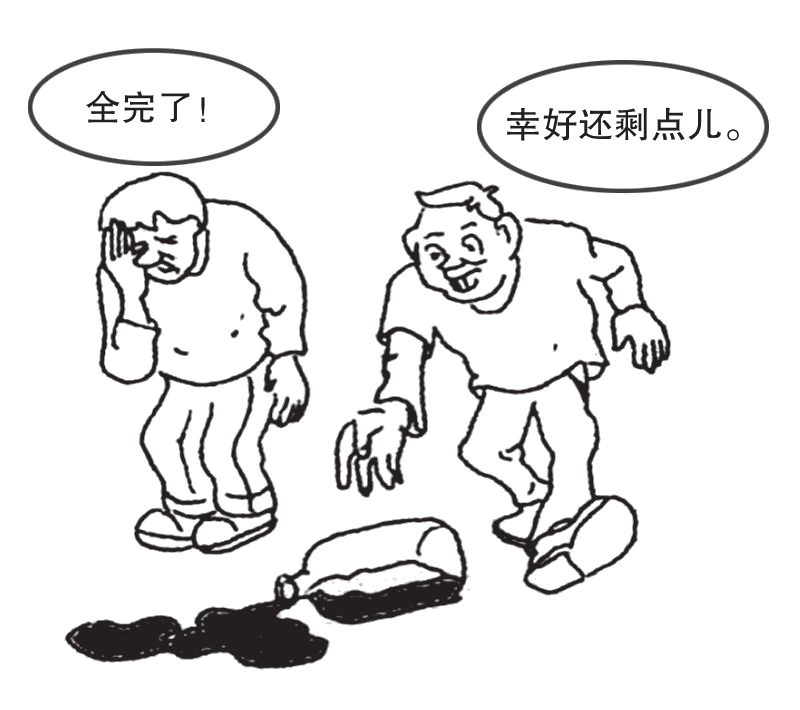
\includegraphics[width=0.45\linewidth]{picture/2012.png}
\end{figure}



\checkpagenumber%

\bta{2013}



\section{Use of English}

\noindent
\textbf{Directions:}\\
Read the following text. Choose the best word (s) for each
	numbered blank and mark A, B, C or D on \textbf{ANSWER SHEET 1}. (10 points)



\TiGanSpace


People are, on the whole, poor at considering background information
when making individual decisions. At first glance this might seem like a
strength that \cloze the ability to make judgments which are
unbiased by \cloze factors. But Dr. Uri Simonsohn speculated that
an inability to consider the big \cloze was leading
decision-makers to be biased by the daily samples of information they
were working with. \cloze , he theorised that a
judge \cloze of appearing too soft \cloze crime might be
more likely to send someone to prison \cloze he had already
sentenced five or six other defendants only to forced community service
on that day.

To \cloze this idea, he turned to the university-admissions
process. In theory, the \cloze of an applicant should not depend
on the few others \cloze randomly for interview during the same
day, but Dr. Simonsoho suspected the truth was \cloze.

He studied the results of 9, 323 MBA interviews \cloze by 31
admissions officers. The interviewers had \cloze applicants on a
scale of one to five. This scale \cloze numerous factors into
consideration. The scores were \cloze used in conjunction with
an applicant's score on the Graduate Management Admission Test, or GMAT,
a standardized exam which is \cloze out of 800 points, to make a
decision on whether to accept him or her.

Dr. Simonsohn found if the score of the previous candidate in a daily
series of interviewees was 0.75 points or more higher than that of the
one \cloze that, then the score for the next applicant
would \cloze by an average of 0.075 points. This might sound
small, but to \cloze the effects of such a decrease a candidate
would need 30 more GMAT points than would otherwise have
been \cloze.



\newpage

\begin{enumerate}
	%\renewcommand{\labelenumi}{\arabic{enumi}.}
	% A(\Alph) a(\alph) I(\Roman) i(\roman) 1(\arabic)
	%设定全局标号series=example	%引用全局变量resume=example
	%[topsep=-0.3em,parsep=-0.3em,itemsep=-0.3em,partopsep=-0.3em]
	%可使用leftmargin调整列表环境左边的空白长度 [leftmargin=0em]
	\item


\fourchoices
{grants}
{submits}
{transmits}
{delivers}




\item


\fourchoices
{minor}
{objective}
{crucial}
{external}




\item


\fourchoices
{issue}
{vision}
{picture}
{moment}




\item


\fourchoices
{For example}
{On average}
{In principle}
{Above all}





\item


\fourchoices
{fond}
{fearful}
{capable}
{thoughtless}




\item


\fourchoices
{in}
{on}
{to}
{for}






\item


\fourchoices
{if}
{until}
{though}
{unless}




\item


\fourchoices
{promote}
{emphasize}
{share}
{test}




\item


\fourchoices
{decision}
{quality}
{status}
{success}




\item


\fourchoices
{chosen}
{studied}
{found}
{identified}




\item

\fourchoices
{exceptional}
{defensible}
{replaceable}
{otherwise}


\item


\fourchoices
{inspired}
{expressed}
{conducted}
{secured}




\item


\fourchoices
{assigned}
{rated}
{matched}
{arranged}




\item


\fourchoices
{put}
{got}
{gave}
{took}





\item


\fourchoices
{instead}
{then}
{ever}
{rather}




\item


\fourchoices
{selected}
{passed}
{marked}
{introduced}




\item


\fourchoices
{before}
{after}
{above}
{below}







\item


\fourchoices
{jump}
{float}
{drop}
{fluctuate}



\item


\fourchoices
{achieve}
{undo}
{maintain}
{disregard}




\item


\fourchoices
{promising}
{possible}
{necessary}
{helpful}

\end{enumerate}


\vfil

\section{Reading Comprehension}


\noindent
\textbf{Part A}\\
\textbf{Directions:}\\
Read the following four texts. Answer the questions below each
	text by choosing A, B, C or
	D. Mark your answers on \textbf{ANSWER SHEET 1}. (40
	points)

\newpage
\subsection{Text 1}


In the 2006 film version of \emph{The Devil Wears Prada}, Miranda
Priestly, played by Meryl Streep, scolds her unattractive assistant for
imagining that high fashion doesn't affect her. Priestly explains how
the deep blue color of the assistant's sweater descended over the years
from fashion shows to department stores and to the bargain bin in which
the poor girl doubtless found her garment.

This top-down conception of the fashion business couldn't be more out of
date or at odds with the feverish world described
in \emph{Overdressed,} Elizabeth Cline's
three-year \uline{indictment} of ``fast fashion''. In the last
decade or so, advances in technology have allowed mass-market labels
such as Zara, H\&M, and Uniqlo to react to trends more quickly and
anticipate demand more precisely. Quicker turnarounds mean less wasted
inventory, more frequent releases, and more profit. These labels
encourage style-conscious consumers to see clothes as disposable---meant
to last only a wash or two, although they don't advertise that---and to
renew their wardrobe every few weeks. By offering on-trend items at
dirt-cheap prices, Cline argues, these brands have hijacked fashion
cycles, shaking an industry long accustomed to a seasonal pace.

The victims of this revolution, of course, are not limited to designers.
For H\&M to offer a \$5.95 knit miniskirt in all its 2, 300-plus stores
around the world, it must rely on low-wage overseas labor, order in
volumes that strain natural resources, and use massive amounts of
harmful chemicals.

\emph{Overdressed} is the fashion world's answer to consumer-activist
bestsellers like Michael Pollan's \emph{The Omnivore's Dilemma}.
``Mass-produced clothing, like fast food, fills a hunger and need, yet
is non-durable and wasteful,'' Cline argues. Americans, she finds, buy
roughly 20 billion garments a year---about 64 items per person---and no
matter how much they give away, this excess leads to waste.

Towards the end of \emph{Overdressed}, Cline introduced her ideal, a
Brooklyn woman named Sarah Kate Beaumont, who since 2008 has made all of
her own clothes---and beautifully. But as Cline is the first to note, it
took Beaumont decades to perfect her craft; her example can't be knocked
off.

Though several fast-fashion companies have made efforts to curb their
impact on labor and the environment---including H\&M, with its green
Conscious Collection line---Cline believes lasting change can only be
effected by the customer. She exhibits the idealism common to many
advocates of sustainability, be it in food or in energy. Vanity is a
constant; people will only start shopping more sustainably when they
can't afford not to.



\begin{enumerate}[resume]
	%\renewcommand{\labelenumi}{\arabic{enumi}.}
	% A(\Alph) a(\alph) I(\Roman) i(\roman) 1(\arabic)
	%设定全局标号series=example	%引用全局变量resume=example
	%[topsep=-0.3em,parsep=-0.3em,itemsep=-0.3em,partopsep=-0.3em]
	%可使用leftmargin调整列表环境左边的空白长度 [leftmargin=0em]
	\item
Priestly criticizes her assistant for her \lineread.


\fourchoices
{poor bargaining skill}
{insensitivity to fashion}
{obsession with high fashion}
{lack of imagination}


\item
According to Cline, mass-market labels urge consumers to \lineread.


\fourchoices
{combat unnecessary waste}
{shut out the feverish fashion world}
{resist the influence of advertisements}
{shop for their garments more frequently}





\item
The word ``indictment'' (Line 3, Para. 2) is closest in
meaning to \lineread.


\fourchoices
{accusation}
{enthusiasm}
{indifference}
{tolerance}


\item
Which of the following can be inferred from the last
paragraph?


\fourchoices
{Vanity has more often been found in idealists.}
{The fast-fashion industry ignores sustainability.}
{People are more interested in unaffordable garments.}
{Pricing is vital to environment-friendly purchasing.}



\item
What is the subject of the text?


\fourchoices
{Satire on an extravagant lifestyle.}
{Challenge to a high-fashion myth.}
{Criticism of the fast-fashion industry.}
{Exposure of a mass-market secret}

\end{enumerate}

\newpage
\subsection{Text 2}


An old saying has it that half of all advertising budgets are
wasted---the trouble is, no one knows which half. In the internet age,
at least in theory, this fraction can be much reduced. By watching what
people search for, click on and say online, companies can aim
``behavioral'' ads at those most likely to buy.

In the past couple of weeks a quarrel has illustrated the value to
advertisers of such fine-grained information: Should advertisers assume
that people are happy to be tracked and sent behavioral ads? Or should
they have explicit permission?

In December 2010 America's Federal Trade Commission (FTC) proposed
adding a ``do not track'' (DNT) option to internet browsers, so that
users could tell advertisers that they did not want to be followed.
Microsoft's Internet Explorer and Apple's Safari both offer DNT;
Google's Chrome is due to do so this year. In February the FTC and
Digital Advertising Alliance (DAA) agreed that \uline{the
	industry} would get cracking on responding to DNT requests.

On May 31st Microsoft set off the row. It said that InternetExplorer 10,
the version due to appear with Windows 8, would have DNT as a default.

Advertisers are horrified. Human nature being what it is, most people
stick with default settings. Few switch DNT on now, but if tracking is
off it will stay off. Bob Liodice, the chief executive of the
Association of National Advertisers, says consumers will be worse off if
the industry cannot collect information about their preferences. People
will not get fewer ads, he says, ``they'll get less meaningful, less
targeted ads.''

It is not yet clear how advertisers will respond. Getting a DNT signal
does not oblige anyone to stop tracking, although some companies have
promised to do so. Unable to tell whether someone really objects to
behavioral ads or whether they are sticking with Microsoft's default,
some may ignore a DNT signal and press on anyway.

Also unclear is why Microsoft has gone it alone. After all, it has an ad
business too, which it says will comply with DNT requests, though it is
still working out how. If it is trying to upset Google, which relies
almost wholly on advertising, it has chosen an indirect method: There is
no guarantee that DNT by default will become the norm. DNT does not seem
an obviously huge selling point for Windows 8---though the firm has
compared some of its other products favorably with Google's on that
count before. Brendon Lynch, Microsoft's chief privacy officer, blogged:
``we believe consumers should have more control.'' Could it really be
that simple?



\begin{enumerate}[resume]
	%\renewcommand{\labelenumi}{\arabic{enumi}.}
	% A(\Alph) a(\alph) I(\Roman) i(\roman) 1(\arabic)
	%设定全局标号series=example	%引用全局变量resume=example
	%[topsep=-0.3em,parsep=-0.3em,itemsep=-0.3em,partopsep=-0.3em]
	%可使用leftmargin调整列表环境左边的空白长度 [leftmargin=0em]
	\item
 It is suggested in paragraph 1 that ``behavioral'' ads help
advertisers to \lineread.


\fourchoices
{ease competition among themselves}
{lower their operational costs}
{avoid complaints from consumers}
{provide better online services}


\item
``The industry'' (Line 5, Para. 3) refers to \lineread.


\fourchoices
{online advertisers}
{e-commerce conductors}
{digital information analysts}
{internet browser developers}



\item
Bob Liodice holds that setting DNT as a default \lineread.


\fourchoices
{may cut the number of junk ads}
{fails to affect the ad industry}
{will not benefit consumers}
{goes against human nature}


\item
 Which of the following is true according to Paragraph 6?


\fourchoices
{DNT may not serve its intended purpose}
{Advertisers are willing to implement DNT}
{DNT is losing its popularity among consumers}
{Advertisers are obliged to offer behavioral ads}





\item
The author's attitude towards what Brendon Lynch said in his
blog is one of \lineread.


\fourchoices
{indulgence}
{understanding}
{appreciation}
{skepticism}


\end{enumerate}


\newpage
\subsection{Text 3}


Up until a few decades ago, our visions of the future were
largely---though by no means uniformly---glowingly positive. Science and
technology would cure all the ills of humanity, leading to lives of
fulfillment and opportunity for all.

Now utopia has grown unfashionable, as we have gained a deeper
appreciation of the range of threats facing us, from asteroid strike to
epidemic flu to climate change. You might even be tempted to assume that
humanity has little future to look forward to.

But such gloominess is misplaced. The fossil record shows that many
species have endured for millions of years---so why shouldn't we? Take a
broader look at our species' place in the universe, and it becomes clear
that we have an excellent chance of surviving for tens, if not hundreds,
of thousands of years. Look up \emph{Homo sapiens} in the ``Red List''
of threatened species of the international Union for the Concentration
of Nature (IUCN), and you will read: ``Listed as Least Concern as the
species is very widely distributed, adaptable, currently increasing, and
there are no major threats resulting in an overall population decline.''

So what does our deep future hold? A growing number of researchers and
organizations are now thinking seriously about that question. For
example, the Long Now Foundation has as its flagship project a
mechanical clock that is designed to still be marking time thousands of
years hence.

Perhaps willfully, it may be easier to think about such lengthy
timescales than about the more immediate future. The potential evolution
of today's technology, and its social consequences, is dazzlingly
complicated, and it's perhaps best left to science fiction writers and
futurologists to explore the many possibilities we can envisage. That's
one reason why we have
launched \emph{Arc}, a new publication
dedicated to the near future.

But take a longer view and there is a surprising amount that we can say
with considerable assurance. As so often, the past holds the key to the
future: we have now identified enough of the long-term patterns shaping
the history of the planet, and our species, to make evidence-based
forecasts about the situations in which our descendants will find
themselves.

This long perspective makes the pessimistic view of our prospects seem
more likely to be a passing fad. To be sure, the future is not all rosy.
But we are now knowledgeable enough to reduce many of the risks that
threatened the existence of earlier humans, and to improve the lot of
those to come.

\begin{enumerate}[resume]
	%\renewcommand{\labelenumi}{\arabic{enumi}.}
	% A(\Alph) a(\alph) I(\Roman) i(\roman) 1(\arabic)
	%设定全局标号series=example	%引用全局变量resume=example
	%[topsep=-0.3em,parsep=-0.3em,itemsep=-0.3em,partopsep=-0.3em]
	%可使用leftmargin调整列表环境左边的空白长度 [leftmargin=0em]
	\item
Our vision of the future used to be inspired by \lineread.


\fourchoices
{our desire for lives of fulfillment}
{our faith in science and technology}
{our awareness of potential risks}
{our belief in equal opportunity}


\item
The IUCN's ``Red List'' suggests that human beings are \lineread.


\fourchoices
{a sustained species}
{a threat to the environment}
{the world's dominant power}
{a misplaced race}



\item
Which of the following is true according to Paragraph 5?


\fourchoices
{\emph{Arc} helps limit the scope of futurological studies.}
{Technology offers solutions to social problems.}
{The interest in science fiction is on the rise.}
{Our immediate future is hard to conceive.}



\item
To ensure the future of mankind, it is crucial to \lineread.


\fourchoices
{explore our planet's abundant resources}
{adopt an optimistic view of the world}
{draw on our experience from the past}
{curb our ambition to reshape history}


\item
Which of the following would be the best title for the
text?


\fourchoices
{Uncertainty about Our Future}
{Evolution of the Human Species}
{The Ever-bright Prospects of Mankind.}
{Science, Technology and Humanity.}

\end{enumerate}



\newpage
\subsection{Text 4}


On a five to three vote, the Supreme Court knocked out much of Arizona's
immigration law Monday---a modest policy victory for the Obama
Administration. But on the more important matter of the Constitution,
the decision was an 8-0 defeat for the Administration's effort to upset
the balance of power between the federal government and the states.

In Arizona v. United States, the majority overturned three of the
four contested provisions of Arizona's controversial plan to have state
and local police enforce federal immigration law. The Constitutional
principles that Washington alone has the power to ``establish a uniform
Rule of Naturalization'' and that federal laws precede state laws are
noncontroversial. Arizona had attempted to fashion state policies that
ran parallel to the existing federal ones.

Justice Anthony Kennedy, joined by Chief Justice John Roberts and the
Court's liberals, ruled that the state flew too close to the federal
sun. On the overturned provisions the majority held that Congress had
deliberately ``occupied the field'' and Arizona has thus intruded on the
federal's privileged powers.

However, the Justices said that Arizona police would be allowed to
verify the legal status of people who come in contact with law
enforcement. That's because Congress has always envisioned joint
federal-state immigration enforcement and explicitly encourages state
officers to share information and cooperate with federal colleagues.

Two of the three objecting Justices---Samuel Alito and Clarence
Thomas---agreed with this Constitutional logic but disagreed about which
Arizona rules conflicted with the federal statute. The only major
objection came from Justice Antonin Scalia, who offered an even more
robust defense of state privileges going back to the Alien and Sedition
Acts.

The 8-0 objection to President Obama turns on what Justice Samuel Alito
describes in his objection as ``a shocking assertion of federal
executive power''. The White House argued that Arizona's laws conflicted
with its enforcement priorities, even if state laws complied with
federal statutes to the letter. In effect, the White House claimed that
it could invalidate any otherwise legitimate state law that it disagrees
with.

Some powers do belong exclusively to the federal government, and control
of citizenship and the borders is among them. But if Congress wanted to
prevent states from using their own resources to check immigration
status, it could. It never did so. The Administration was in essence
asserting that because it didn't want to carry out Congress's
immigration wishes, no state should be allowed to do so either. Every
Justice rightly rejected this remarkable claim.


\begin{enumerate}[resume]
	%\renewcommand{\labelenumi}{\arabic{enumi}.}
	% A(\Alph) a(\alph) I(\Roman) i(\roman) 1(\arabic)
	%设定全局标号series=example	%引用全局变量resume=example
	%[topsep=-0.3em,parsep=-0.3em,itemsep=-0.3em,partopsep=-0.3em]
	%可使用leftmargin调整列表环境左边的空白长度 [leftmargin=0em]
	\item
Three provisions of Arizona's plan were overturned because
they \lineread.


\fourchoices
{deprived the federal police of Constitutional powers}
{disturbed the power balance between different states}
{overstepped the authority of federal immigration law}
{contradicted both the federal and state policies}



\item
On which of the following did the Justices agree, according
to Paragraph 4?


\fourchoices
{Federal officers' duty to withhold immigrants' information.}
{States' independence from federal immigration law.}
{States' legitimate role in immigration enforcement.}
{Congress's intervention in immigration enforcement.}



\item
It can be inferred from Paragraph 5 that the Alien and
Sedition Acts \lineread.


\fourchoices
{violated the Constitution}
{undermined the states' interests}
{supported the federal statute}
{stood in favor of the states}


\item
The White House claims that its power of enforcement \lineread.


\fourchoices
{outweighs that held by the states}
{is dependent on the states' support}
{is established by federal statutes}
{rarely goes against state laws}


\item
What can be learned from the last paragraph?


\fourchoices
{Immigration issues are usually decided by Congress.}
{The Administration is dominant over immigration issues.}
{Justices wanted to strengthen its coordination with Congress.}
{Justices intended to check the power of the Administration.}



	
\end{enumerate}


\newpage

\noindent
\textbf{Part B}\\
\textbf{Directions:}\\
In the following article, some sentences have been removed. For
	Questions 41-45, choose the most suitable one from the list A-G to fit
	into each of the numbered blank. There are two extra choices, which do
	not fit in any of the gaps. Mark your answers on \textbf{ANSWER SHEET 1}. (10 points)


\TiGanSpace


The social sciences are flourishing. As of 2005, there were almost half
a million professional social scientists from all fields in the world,
working both inside and outside academia. According to the \emph{World
	Social Science Report 2010}, the number of social-science students
worldwide has swollen by about 11\% every year since 2000.

Yet this enormous resource is not contributing enough to today's global
challenges, including climate change, security, sustainable development
and health.  
\linefill.
Humanity has
the necessary agro-technological tools to eradicate hunger, from
genetically engineered crops to artificial fertilizers. Here, too, the
problems are social: the organization and distribution of food, wealth
and prosperity.




\linefill. This is a shame---the
community should be grasping the opportunity to raise its influence in
the real world. To paraphrase the great social scientist Joseph
Schumpeter: there is no radical innovation without creative destruction.

Today, the social sciences are largely focused on disciplinary problems
and internal scholarly debates, rather than on topics with external
impact. Analyses reveal that the number of papers including the keywords
``environmental change'' or ``climate change'' have increased rapidly
since 2004. \linefill.

When social scientists do tackle practical issues, their scope is often
local: Belgium is interested mainly in the effects of poverty on
Belgium, for example. And whether the community's work contributes much
to an overall accumulation of knowledge is doubtful.

The problem is not necessarily the amount of available funding. \linefill. This is an adequate amount so
long as it is aimed in the right direction. Social scientists who
complain about a lack of funding should not expect more in today's
economic climate.

The trick is to direct these funds better. The European Union Framework
funding programs have long had a category specifically targeted at
social scientists. This year, it was proposed that the system be
changed: Horizon 2020, a new program to be enacted in 2014, would not
have such a category. This has resulted in protests from social
scientists. But the intention is not to neglect social science; rather,
the complete opposite. \linefill.
That should create more collaborative endeavors and help to develop
projects aimed directly at solving global problems.

\begin{listmatch}
	%\renewcommand{\labelenumi}{\arabic{enumi}.}
	% A(\Alph) a(\alph) I(\Roman) i(\roman) 1(\arabic)
	%设定全局标号series=example	%引用全局变量resume=example
	%[topsep=-0.3em,parsep=-0.3em,itemsep=-0.3em,partopsep=-0.3em]
	%可使用leftmargin调整列表环境左边的空白长度 [leftmargin=0em]
	\item
 It could be that we are evolving two communities of social
scientists: one that is discipline-oriented and publishing in highly
specialized journals, and one that is problem-oriented and publishing
elsewhere, such as policy briefs.


\item 
 However, the numbers are still small: in 2010, about 1, 600 of
the 100, 000 social-sciences papers published globally included one of
these keywords.

\item 
The idea is to force social scientists to integrate their work
with other categories, including health and demographic change; food
security; marine research and the bio-economy, clean, efficient energy;
and inclusive, innovative and secure societies.





\item 
The solution is to change the mindset of the academic community,
and what it considers to be its main goal. Global challenges and social
innovation ought to receive much more attention from scientists,
especially the young ones.

\item 
These issues all have root causes in human behavior: all require
behavioral change and social innovations, as well as technological
development. Stemming climate change, for example, is as much about
changing consumption patterns and promoting tax acceptance as it is
about developing clean energy.


\item 
Despite these factors, many social scientists seem reluctant to
tackle such problems. And in Europe, some are up in arms over a proposal
to drop a specific funding category for social-science research and to
integrate it within cross-cutting topics of sustainable development.




\item 
During the late 1990s , national spending on social sciences and
the humanities as a percentage of all research and development
funds---including government, higher education, non-profit and
corporate---varied from around 4\% to 25\%; in most European nations, it
is about 15\%.








\end{listmatch}



\newpage
\noindent
\textbf{Part C}\\
\textbf{Directions:}\\
Read the following text carefully and then translate the
	underlined segments into Chinese. Your translation should be written
	clearly on \textbf{ANSWER SHEET 2}. (10 points)



\TiGanSpace



It is speculated that gardens arise from a basic human need in the
individuals who made them: the need for creative expression. There is no
doubt that gardens evidence an irrepressible urge to create, express,
fashion, and beautify and that self-expression is a basic human urge;
\transnum \uline{yet when one looks at the photographs of the garden
	created by the homeless, it strikes one that , for all their diversity of
	styles, these gardens speak of various other fundamental urges, beyond
	that of decoration and creative expression.}

One of these urges has to do with creating a state of peace in the midst
of turbulence, a ``still point of the turning world,'' to borrow a
phrase from T. S. Eliot. \transnum \uline{A sacred place of peace,
	however crude it may be, is a distinctly human need, as opposed to
	shelter, which is a distinctly animal need.} This distinction is so much
so that where the latter is lacking, as it is for these unlikely
gardens, the former becomes all the more urgent. Composure is a state of
mind made possible by the structuring of one's relation to one's
environment. \transnum \uline{The gardens of the homeless, which are in
	effect homeless gardens, introduce form into an
	urban environment where it either didn't exist or was not discernible as
	such.} In so doing they give composure to a segment of the inarticulate
environment in which they take their stand.

Another urge or need that these gardens appear to respond to, or to
arise from, is so intrinsic that we are barely ever conscious of its
abiding claims on us. When we are deprived of green, of plants, of
trees, \transnum \uline{ most of us give in to a demoralization of spirit
	which we usually blame on some psychological conditions, until one day
	we find ourselves in a garden and feel the oppression vanish as if by
	magic.} In most of the homeless gardens of New York City the actual
cultivation of plants is unfeasible, yet even so the compositions often
seem to represent attempts to call forth the spirit of plant and animal
life, if only symbolically, through a clumplike arrangement of
materials, an introduction of colors, small pools of water, and a
frequent presence of petals or leaves as well as of stuffed animals. On
display here are various fantasy elements whose reference, at some basic
level, seems to be the natural world. \transnum \uline{It is this
	implicit or explicit reference to nature that fully justifies the use of
	the word garden, though in a ``liberated''
	sense, to describe these synthetic constructions.} In them we can see
biophilia---a yearning for contact with nonhuman life---assuming uncanny
representational forms.

\newpage

\section{Writing}


\noindent
\textbf{Part A}\\
\textbf{51. Directions:}

Write an e-mail of about 100 words to a foreign teacher in your college,
inviting him/her to be a judge for the upcoming English speech contest.

You should include the details you think necessary.

You should write neatly on the ANSWER SHEET 2.

\textbf{Do not} sign your own name at the end of the e-mail. Use ``Li Ming''
instead.

\textbf{Do not} write the address. (10 points)



\vspace{3em}

\noindent
\textbf{Part B}\\
\textbf{52. Directions:}

Write an essay of 160-200 words based on the following drawing. In your
essay you should
\begin{listwrite}
	%\renewcommand{\labelenumi}{\arabic{enumi}.}
	% A(\Alph) a(\alph) I(\Roman) i(\roman) 1(\arabic)
	%设定全局标号series=example	%引用全局变量resume=example
	%[topsep=-0.3em,parsep=-0.3em,itemsep=-0.3em,partopsep=-0.3em]
	%可使用leftmargin调整列表环境左边的空白长度 [leftmargin=0em]
	\item
	describe the drawing briefly

\item 
 explain its intended meaning, and

\item 
 give your comments.
\end{listwrite}

You should write neatly on the ANSWER SHEET 2. (20 points)


\begin{figure}[h!]
	\centering
	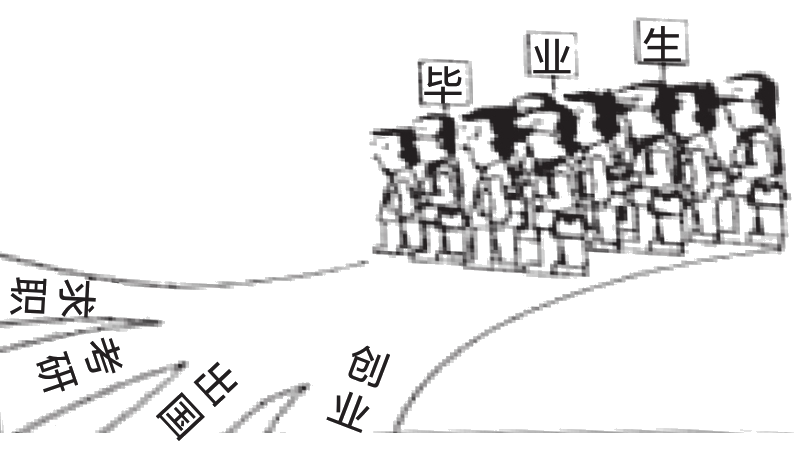
\includegraphics[width=0.56\linewidth]{picture/2013.png}
	\caption*{选择}
\end{figure}

\checkpagenumber%

\bta{2014}


\section{ Use of English}

\textbf{Directions:}\\
 Read the following text. Choose the best word (s) for
	each numbered blank and mark A, B, C or D on \textbf{ANSWER SHEET 1}. (10
	points)



\TiGanSpace



As many people hit middle age, they often start to notice that their
memory and mental clarity are not what they used to be. We suddenly
can't remember \cloze we put the keys just a moment ago, or an
old acquaintance's name, or the name of an old band we used to love. As
the brain \cloze , we refer to these occurrences as " senior
moments." \cloze seemingly innocent, this loss of mental focus
can potentially have a(an) \cloze impact on our professional,
social, and personal \cloze.

Neuroscientists, experts who study the nervous system, are increasingly
showing that there's actually a lot that can be done. It \cloze
out that the brain needs exercise in much the same way our muscles do,
and the right mental \cloze can significantly improve our basic
cognitive \cloze. Thinking is essentially a \cloze of
making connections in the brain. To a certain extent, our ability to
\cloze in making the connections that drive intelligence is
inherited. \cloze , because these connections are made through
effort and practice, scientists believe that intelligence can expand and
fluctuate \cloze mental effort.

Now, a new Web-based company has taken it a step \cloze and
developed the first ``brain training program'' designed to actually help
people improve and regain their mental \cloze.

The Web-based program \cloze you to systematically improve your
memory and attention skills. The program keeps \cloze of your
progress and provides detailed feedback \cloze your performance
and improvement. Most importantly, it \cloze modifies and
enhances the games you play to \cloze on the strengths you are
developing--much like a(n) \cloze exercise routine requires
you to increase resistance and vary your muscle use.


\newpage

\begin{enumerate}
	%\renewcommand{\labelenumi}{\arabic{enumi}.}
	% A(\Alph) a(\alph) I(\Roman) i(\roman) 1(\arabic)
	%设定全局标号series=example	%引用全局变量resume=example
	%[topsep=-0.3em,parsep=-0.3em,itemsep=-0.3em,partopsep=-0.3em]
	%可使用leftmargin调整列表环境左边的空白长度 [leftmargin=0em]
	\item


\fourchoices
{why}
{when}
{that}
{where}




\item


\fourchoices
{improves}
{fades}
{collapses}
{recovers}




\item


\fourchoices
{While}
{Unless}
{Once}
{If}




\item


\fourchoices
{uneven}
{limited}
{damaging}
{obscure}




\item

\fourchoices
{relationship}
{environment}
{wellbeing}
{outlook}



\item


\fourchoices
{turns}
{finds}
{points}
{figures}




\item

\fourchoices
{responses}
{roundabouts}
{workouts}
{associations}



\item

\fourchoices
{genre}
{criterion}
{circumstances}
{functions}



\item


\fourchoices
{channel}
{process}
{sequence}
{condition}




\item


\fourchoices
{excel}
{feature}
{persist}
{believe}




\item


\fourchoices
{However}
{Moreover}
{Otherwise}
{Therefore}




\item

\fourchoices
{instead of}
{regardless of}
{apart from}
{according to}


\item


\fourchoices
{back}
{further}
{aside}
{around}




\item

\fourchoices
{framework}
{stability}
{sharpness}
{flexibility}


\item


\fourchoices
{hurries}
{reminds}
{forces}
{allows}




\item


\fourchoices
{order}
{track}
{hold}
{pace}




\item


\fourchoices
{to}
{on}
{for}
{with}




\item

\fourchoices
{constantly}
{habitually}
{irregularly}
{unusually}



\item


\fourchoices
{carry}
{put}
{build}
{take}




\item


\fourchoices
{risky}
{familiar}
{idle}
{effective}

\end{enumerate}


\vfil

\section{Reading Comprehension}


\noindent
\textbf{Part A}\\
\textbf{Directions:}\\
 Read the following four texts. Answer the questions
	after each text by choosing A, B, C or
	D. Mark your answers on \textbf{ANSWER SHEET 1}. (40 points)

\newpage
\subsection{Text 1}


In order to ``change lives for the better'' and reduce ``dependency,''
George Osbome, Chancellor of the Exchequer, introduced the ``upfront
work search'' scheme. Only if the jobless arrive at the jobcentre with
a CV, register for online job search, and start looking for work will
they be eligible for benefit---and then they should report weekly rather
than fortnightly. What could be more reasonable?

More apparent reasonableness followed. There will now be a seven-day
wait for the jobseeker's allowance. ``Those first few days should be
spent looking for work, not looking  \uline{to sign on},'' he
claimed. ``We're doing these things because we know they help people stay
off benefits and help those on benefits get into work faster.'' Help?
Really? On first hearing, this was the socially concerned chancellor,
trying to change lives for the better, complete with ``reforms'' to an
obviously indulgent system that demands too little effort from the newly
unemployed to find work, and subsidises laziness. What motivated him, we
were to understand, was his zeal for ``fundamental fairness''---protecting
the taxpayer, controlling spending and ensuring that only the most
deserving claimants received their benefits.

Losing a job is hurting: you don't skip down to the jobcentre with a
song in your heart, delighted at the prospect of doubling your income
from the generous state. It is financially terrifying, psychologically
embarrassing and you know that support is minimal and extraordinarily
hard to get. You are now not wanted; you support is minimal and
extraordinarily hard to get. You are now not wanted; you are now
excluded from the work environment that offers purpose and structure in
your life. Worse, the crucial income to feed yourself and your family
and pay the bills has disappeared. Ask anyone newly unemployed what they
want and the answer is always: a job.

But in Osborneland, your first instinct is to fall into dependency---permanent dependency if you can get it---supported by a state only too
ready to indulge your falsehood. It is as though 20 years of ever-tougher reforms of the job search and benefit administration system
never happened. The principle of British welfare is no longer that you
can insure yourself against the risk of unemployment and receive
unconditional payments if the disaster happens. Even the very phrase
``jobseeker's allowance'' is about redefining the
unemployed as a ``jobseeker'' who had no fundamental right to a benefit he
or she has earned through making national insurance contributions.
Instead, the claimant receives a time-limited ``allowance,'' conditional
on actively seeking a job; no entitlement and no insurance, at £71.70 a
week, one of the least generous in the EU.


\begin{enumerate}[resume]
	%\renewcommand{\labelenumi}{\arabic{enumi}.}
	% A(\Alph) a(\alph) I(\Roman) i(\roman) 1(\arabic)
	%设定全局标号series=example	%引用全局变量resume=example
	%[topsep=-0.3em,parsep=-0.3em,itemsep=-0.3em,partopsep=-0.3em]
	%可使用leftmargin调整列表环境左边的空白长度 [leftmargin=0em]
	\item
George Osborne's scheme was intended to \lineread.


\fourchoices
{provide the unemployed with easier access to benefits}
{encourage jobseekers' active engagement in job seeking}
{motivate the unemployed to report voluntarily}
{guarantee jobseekers' legitimate right to benefits}


\item
 The phrase ``to sign on'' (Line 3, Para. 2) most probably
means \lineread.


\fourchoices
{to check on the availability of jobs at the jobcentre}
{to accept the government's restrictions on the allowance}
{to register for an allowance from the government}
{to attend a governmental job-training program}



\item
What prompted the chancellor to develop his scheme?


\fourchoices
{A desire to secure a better life for all.}
{An eagerness to protect the unemployed.}
{An urge to be generous to the claimants.}
{A passion to ensure fairness for taxpayers.}


\item
According to Paragraph 3, being unemployed makes one feel \lineread.



\fourchoices
{uneasy}
{enraged}
{insulted}
{guilty}




\item
To which of the following would the author most probably
agree?


\fourchoices
{The British welfare system indulges jobseekers' laziness.}
{Osborne's reforms will reduce the risk of unemployment.}
{The jobseekers' allowance has met their actual needs.}
{Unemployment benefits should not be made conditional.}


\end{enumerate}



\newpage
\subsection{Text 2}


All around the world, lawyers generate more hostility than the members
of any other profession---with the possible exception of journalism.
But there are few places where clients have more grounds for complaint
than America.

During the decade before the economic crisis, spending on legal services
in America grew twice as fast as inflation. The best lawyers made
skyscrapers-full of money, tempting ever more students to pile into law
schools. But most law graduates never get a big-firm job. Many of them
instead become the kind of nuisance-lawsuit filer that makes the tort
system a costly nightmare.

There are many reasons for this. One is the excessive costs of a legal
education. There is just one path for a lawyer in most American states:
a four-year undergraduate degree in some unrelated subjects, then a
three-year law degree at one of 200 law schools authorized by the
American Bar Association and an expensive preparation for the bar exam.
This leaves today's average law-school graduate with \$100, 000 of debt
on top of undergraduate debts. Law-school debt means that they have to
work fearsomely hard.

Reforming the system would help both lawyers and their customers.
Sensible ideas have been around for a long time, but the state-level
bodies that govern the profession have been too conservative to
implement them. One idea is to allow people to study law as an
undergraduate degree. Another is to let students sit for the bar after
only two years of law school. If the bar exam is truly a stern enough
test for a would-be lawyer, those who can sit it earlier should be
allowed to do so. Students who do not need the extra training could cut
their debt mountain by a third.

The other reason why costs are so high is the restrictive guild-like
ownership structure of the business. Except in the District of Columbia,
non-lawyers may not own any share of a law firm. This keeps fees high
and innovation slow. There is pressure for change from within the
profession, but opponents of change among the regulators insist that
keeping outsiders out of a law firm isolates lawyers from the pressure
to make money rather than serve clients ethically.

In fact, allowing non-lawyers to own shares in law firms would reduce
costs and improve services to customers, by encouraging law firms to use
technology and to employ professional managers to focus on improving
firms' efficiency. After all, other countries, such as Australia and
Britain, have started liberalizing their legal professions. America
should follow.


\begin{enumerate}[resume]
	%\renewcommand{\labelenumi}{\arabic{enumi}.}
	% A(\Alph) a(\alph) I(\Roman) i(\roman) 1(\arabic)
	%设定全局标号series=example	%引用全局变量resume=example
	%[topsep=-0.3em,parsep=-0.3em,itemsep=-0.3em,partopsep=-0.3em]
	%可使用leftmargin调整列表环境左边的空白长度 [leftmargin=0em]
	\item
 A lot of students take up law as their profession due to \lineread.


\fourchoices
{the growing demand from clients}
{the increasing pressure of inflation}
{the prospect of working in big firms}
{the attraction of financial rewards}



\item
Which of the following adds to the costs of legal education
in most American states?


\fourchoices
{Higher tuition fees for undergraduate studies.}
{Admissions approval from the bar association.}
{Pursuing a bachelor's degree in another major.}
{Receiving training by professional associations.}


\item
Hindrance to the reform of the legal system originates from \lineread.


\fourchoices
{lawyers' and clients' strong resistance}
{the rigid bodies governing the profession}
{the stern exam for would-be lawyers}
{non-professionals' sharp criticism}

\item
The guild-like ownership structure is considered
	``restrictive'' partly because it \lineread.


\fourchoices
{bans outsiders' involvement in the profession}
{keeps lawyers from holding law-firm shares}
{aggravates the ethical situation in the trade}
{prevents lawyers from gaining due profits}



\item
In this text, the author mainly discusses \lineread.


\fourchoices
{flawed ownership of America's law firms and its causes}
{the factors that help make a successful lawyer in America}
{a problem in America's legal profession and solutions to it}
{the role of undergraduate studies in America's legal education}

	
\end{enumerate}


\newpage
\subsection{Text 3}


The US \$3--million Fundamental Physics Prize is indeed an interesting
experiment, as Alexander Polyakov said when he accepted this year's
award in March. And it is far from the only one of its type. As a News
Feature article in \emph{Nature} discusses, a string of lucrative awards
for researchers have joined the Nobel Prizes in recent years. Many, like
the Fundamental Physics Prize, are funded from the
telephone-number-sized bank accounts of Internet entrepreneurs. These
benefactors have succeeded in their chosen fields, they say, and they
want to use their wealth to draw attention to those who have succeeded
in science.

What's not to like? Quite a lot, according to a handful of scientists
quoted in the News Feature. You cannot buy class, as the old saying
goes, and these upstart entrepreneurs cannot buy their prizes the
prestige of the Nobels. The new awards are an exercise in self-promotion
for those behind them, say scientists. They could distort the
achievement-based system of peer-review-led research. They could cement
the status quo of peer-reviewed research. They do not fund peer-reviewed
research. They perpetuate the myth of the lone genius.

The goals of the prize-givers seem as scattered as the criticism. Some
want to shock, others to draw people into science, or to better reward
those who have made their careers in research.

As \emph{Nature} has pointed out before, there are some legitimate concerns
about how science prizes---both new and old---are distributed. The
Breakthrough Prize in Life Sciences, launched this year, takes an
unrepresentative view of what the life sciences include. But the Nobel
Foundation's limit of three recipients per prize, each of whom must
still be living, has long been outgrown by the collaborative nature of
modern research---as will be demonstrated by the inevitable row over who
is ignored when it comes to acknowledging the discovery of the Higgs
boson. The Nobels were, of course, themselves set up by a very rich
individual who had decided what he wanted to do with his own money.
Time, rather than intention, has given them legitimacy.

As much as some scientists may complain about the new awards, two things
seem clear. First, most researchers would accept such a prize if they
were offered one. Second, it is surely a good thing that the money and
attention come to science rather than go elsewhere, It is fair to
criticize and question the mechanism---that is the culture of research,
after all---but it is the prize-givers' money to do with as they please.
It is wise to take such gifts with gratitude and grace.

\begin{enumerate}[resume]
	%\renewcommand{\labelenumi}{\arabic{enumi}.}
	% A(\Alph) a(\alph) I(\Roman) i(\roman) 1(\arabic)
	%设定全局标号series=example	%引用全局变量resume=example
	%[topsep=-0.3em,parsep=-0.3em,itemsep=-0.3em,partopsep=-0.3em]
	%可使用leftmargin调整列表环境左边的空白长度 [leftmargin=0em]
	\item
The Fundamental Physics Prize is seen as \lineread.


\fourchoices
{a symbol of the entrepreneurs' wealth}
{a possible replacement of the Nobel Prizes}
{an example of bankers' investments}
{a handsome reward for researchers}




\item
The critics think that the new awards will most benefit \lineread.


\fourchoices
{the profit-oriented scientists}
{the founders of the awards}
{the achievement-based system}
{peer-review-led research}


\item
The discovery of the Higgs boson is a typical case which
involves \lineread.


\fourchoices
{controversies over the recipients' status}
{the joint effort of modern researchers}
{legitimate concerns over the new prizes}
{the demonstration of research findings}




\item
According to Paragraph 4, which of the following is true of
the Nobels?


\fourchoices
{Their endurance has done justice to them.}
{Their legitimacy has long been in dispute.}
{They are the most representative honor.}
{History has never cast doubt on them.}






\item
The author believes that the new awards are \lineread.


\fourchoices
{acceptable despite the criticism}
{harmful to the culture of research}
{subject to undesirable changes}
{unworthy of public attention}

\end{enumerate}


\newpage
\subsection{Text 4}


``The Heart of the Matter,'' the just-released report by the American
Academy of Arts and Sciences (AAAS), deserves praise for affirming the
importance of the humanities and social sciences to the prosperity and
security of liberal democracy in America. Regrettably, however, the
report's failure to address the true nature of the crisis facing liberal
education may cause more harm than good.

In 2010, leading congressional Democrats and Republicans sent
letters to the AAAS asking that it identify actions that could be taken
by ``federal, state and local governments, universities, foundations,
educators, individual benefactors and others'' to ``maintain national
excellence in humanities and social scientific scholarship and
education.'' In response, the American Academy formed the Commission on
the Humanities and Social Sciences. Among the commission's 51 members
are top-tier-university presidents, scholars, lawyers, judges, and
business executives, as well as prominent figures from diplomacy,
filmmaking, music and journalism.

The goals identified in the report are generally admirable. Because
representative government presupposes an informed citizenry, the report
supports full literacy; stresses the study of history and government,
particularly American history and American government; and encourages
the use of new digital technologies. To encourage innovation and
competition, the report calls for increased investment in research, the
crafting of coherent curricula that improve students' ability to solve
problems and communicate effectively in the 21st century, increased
funding for teachers and the encouragement of scholars to bring their
learning to bear on the great challenges of the day. The report also
advocates greater study of foreign languages, international affairs and
the expansion of study abroad programs.

Unfortunately, despite 2½ years in the making, ``The Heart of the
Matter'' never gets to the heart of the matter: the illiberal nature of
liberal education at our leading colleges and universities. The
commission ignores that for several decades America's colleges and
universities have produced graduates who don't know the content and
character of liberal education and are thus deprived of its benefits.
Sadly, the spirit of inquiry once at home on campus has been replaced by
the use of the humanities and social sciences as vehicles for
publicizing ``progressive,'' or left-liberal propaganda.

Today, professors routinely treat the progressive interpretation of
history and progressive public policy as the proper subject of study
while portraying conservative or classical liberal ideas---such as free
markets or self-reliance ---as falling outside the boundaries of
routine, and sometimes legitimate, intellectual investigation.

The AAAS displays great enthusiasm for liberal education. Yet its
report may well set back reform by obscuring the depth and breadth of
the challenge that Congress asked it to illuminate.

\begin{enumerate}[resume]
	\item
According to Paragraph 1, what is the author's attitude toward the AAAS's report?



\fourchoices
{Critical}
{Appreciative}
{Contemptuous}
{Tolerant}



\item
Influential figures in the Congress required that the AAAS
report on how to \lineread.


\fourchoices
{retain people's interest in liberal education}
{define the government's role in education}
{keep a leading position in liberal education}
{safeguard individuals' rights to education}

\item
 According to Paragraph 3, the report suggests \lineread.


\fourchoices
{an exclusive study of American history}
{a greater emphasis on theoretical subjects}
{the application of emerging technologies}
{funding for the study of foreign languages}



\item
 The author implies in Paragraph 5 that professors are \lineread.


\fourchoices
{supportive of free markets}
{cautious about intellectual investigation}
{conservative about public policy}
{biased against classical liberal ideas}




\item
 Which of the following would be the best title for the
text?


\fourchoices
{Ways to Grasp ``The Heart of the Matter''}
{Illiberal Education and ``The Heart of the Matter''}
{The AAAS's Contribution to Liberal Education}
{Progressive Policy vs. Liberal Education}



\end{enumerate}


\newpage
\noindent
\textbf{Part B}\\
\textbf{Directions:}\\
The following paragraphs are given in a wrong order. For
	Questions 41-45, you are required to reorganize into a coherent text by
	choosing from the list A-G and filling them into the numbered boxes. Paragraphs A and E have been correctly placed. Mark your answers on the \textbf{ANSWER SHEET}. (10 points)

\begin{listmatch}
	%\renewcommand{\labelenumi}{\arabic{enumi}.}
	% A(\Alph) a(\alph) I(\Roman) i(\roman) 1(\arabic)
	%设定全局标号series=example	%引用全局变量resume=example
	%[topsep=-0.3em,parsep=-0.3em,itemsep=-0.3em,partopsep=-0.3em]
	%可使用leftmargin调整列表环境左边的空白长度 [leftmargin=0em]
	\item
Some archaeological sites have always been easily
observable---for example, the Parthenon in Athens, Greece; the pyramids
of Giza in Egypt; and the megaliths of Stonehenge in southern England.
But these sites are exceptions to the norm. Most archaeological sites
have been located by means of careful searching, while many others have
been discovered by accident. Olduvai Gorge, fell into its deep valley in
1911. Thousands of Aztec artifacts came to light during the digging of
the Mexico City subway in the 1970 s.


\item 
In another case, American archaeologists Rene million and George
Cowgill spent years systematically mapping the entire city of
Teotihuacan in the valley of Mexico near what is now Mexico City. at its
peak around AD 600, this city was one of the largest human settlements
in the word. The researchers mapped not only the city's vast and ornate
ceremonial areas, but also hundreds of simpler apartment complexes where
common people lived.


\item 
How do archaeologists know where to find what they are looking
for when there is nothing visible on the surface of the ground?
Typically, they survey and sample (make test excavations on) large areas
of terrain to determine where excavation will yield useful information.
Surveys and test samples have also become important for understanding
the larger landscapes that contain archaeological sites.


\item 
Surveys can cover a single large settlement or entire
landscapes. In one case, many researchers working around the ancient
Maya city of Copán, Honduras, have located hundreds of small rural
village and individual dwellings by using aerial photographs and by
making surveys on foot. The resulting settlement maps show how the
distribution and density of the rural population around the city changed
dramatically between AD 500 and 850, when Copán collapsed.


\item 
 To find their sites, archaeologists today rely heavily on
systematic survey methods and a variety of high-technology tools and
techniques. Airborne technologies, such as different types of radar and
photographic equipment carried by airplanes or spacecraft, allow
archaeologists to learn about what lies beneath the ground without
digging. Aerial surveys locate general areas of interest or larger
buried features, such as ancient buildings or fields.


\item 
 Most archaeological sites, however, are discovered by
archaeologists who have set out to look for them. Such searches can take
years. British archaeologist Howard Carter knew that the tomb of the
Egyptian pharaoh Tutankhamen existed from information found in other
sites. Carter sifted through rubble in the Valley of the King for seven
years before he located the tomb in 1922. In the late 1800s British
archaeologist Sir Arthur Eyan combed antique dealers' stores in Athens,
Greece. He was searching for thing engraved seals attributed to the
ancient Mycenaean culture that dominated Greece from the 1400s to 1200s
BC. Evas's interpretations of those engravings eventually led them to
find the Minoan palace at Knossos (Knos\'os) on the island of Crete, in 1900.


\item 
 Ground surveys allow archaeologists to pinpoint the places where
digs will be successful. Most ground surveys involve a lot of walking,
looking for surface clues such as small fragments of pottery. They often
include a certain amounts of digging to test for buried materials at
selected points across a landscape. Archaeologists also may locate
buried remains by using such technologies as ground radar,
magnetic-field recording, and metal detector. Archaeologists commonly
use computers to map sites and the landscapes around sites. Two and
three-dimensional maps are helpful tools in planning excavations,
illustrating how sites look, and presenting the results of
archaeological research.


\end{listmatch}


\[ 
\begin{tabular}{|c|c|}
	\hline
	41. &  \hspace{1.5em} \\
	\hline
\end{tabular}
\rightarrow
\begin{tabular}{|c|}
	\hline
	A \\
	\hline
\end{tabular}
\rightarrow
\begin{tabular}{|c|c|}
	\hline
	42. &  \hspace{1.5em} \\
	\hline
\end{tabular}
\rightarrow
\begin{tabular}{|c|}
	\hline
	E \\
	\hline
\end{tabular}
\rightarrow
\begin{tabular}{|c|c|}
	\hline
	43. &  \hspace{1.5em} \\
	\hline
\end{tabular}
\rightarrow
\begin{tabular}{|c|c|}
	\hline
	44. &  \hspace{1.5em} \\
	\hline
\end{tabular}
\rightarrow
\begin{tabular}{|c|c|}
	\hline
	45. &  \hspace{1.5em} \\
	\hline
\end{tabular}
\]


\phantom{ \linefill \linefill \linefill \linefill \linefill}



\newpage

\noindent
\textbf{Part C}\\
\textbf{Directions:}\\
Read the following text carefully and then translate the
	underlined segments into Chinese. Your translation should be written on
	the \textbf{ANSWER SHEET}. (10 points)


\TiGanSpace


Music means different things to different people and sometimes even
different things to the same person at different moments of his life. It
might be poetic, philosophical, sensual, or mathematical, but in any
case it must, in my view, have something to do with the soul of the
human being. Hence it is metaphysical; but the means of expression is
purely and exclusively physical: sound. I believe it is precisely this
permanent coexistence of metaphysical message through physical means
that is the strength of music. \transnum \uline{It is also the reason why
	when we try to describe music with words, all we can do is articulate
	our reactions to it, and not grasp music itself.}

Beethoven's importance in music has been principally defined by the
revolutionary nature of his compositions. He freed music from hitherto
prevailing conventions of harmony and structure. Sometimes I feel in his
late works a will to break all signs of continuity. The music is abrupt
and seemingly disconnected, as in the last piano sonata. In musical
expression, he did not feel restrained by the weight of convention. 
\transnum \uline{By all accounts he was a freethinking person, and a
	courageous one, and I find courage an essential quality for the
	understanding, let alone the performance, of his works.}

This courageous attitude in fact becomes a requirement for the
performers of Beethoven's music. His compositions demand the performer
to show courage, for example in the use of dynamics.
\transnum \uline{Beethoven's habit of increasing the volume with an extreme
	intensity and then abruptly following it with a sudden soft passage was
	only rarely used by composers before him.}

Beethoven was a deeply political man in the broadest sense of the word.
He was not interested in daily politics, but concerned with questions of
moral behavior and the larger questions of right and wrong affecting the
entire society. \transnum  \uline{Especially significant was his view of
	freedom, which, for him, was associated with the rights and
	responsibilities of the individual: he advocated freedom of thought and
	of personal expression.}

Beethoven's music tends to move from chaos to order as if order were an
imperative of human existence. For him, order does not result from
forgetting or ignoring the disorders that plague our existence; order is
a necessary development, an improvement that may lead to the Greek ideal
of spiritual elevation. It is not by chance that the Funeral March is
not the last movement of the Eroica Symphony, but the second, so that
suffering does not have the last word. \transnum \uline{One could
	interpret much of the work of Beethoven by saying that suffering is
	inevitable, but the courage to fight it renders life worth living.}




\newpage
\section{Writing}


\noindent
\textbf{Part A}\\
\textbf{51. Directions:}

Write a letter of about 100 words to the president of your university,
suggesting how to improve students' physical condition.

You should include the details you think necessary.

You should write neatly on the ANSWER SHEET.

\textbf{Do not} sign your own name at the end of the letter. Use ``Li
Ming'' instead.

\textbf{Do not} write the address.(10 points)


\vspace{2em}


\noindent
\textbf{Part B}\\
\textbf{52. Directions:}

Write an essay of 160-200 words based on the following drawing. In your
essay, you should
\begin{listwrite}
	%\renewcommand{\labelenumi}{\arabic{enumi}.}
	% A(\Alph) a(\alph) I(\Roman) i(\roman) 1(\arabic)
	%设定全局标号series=example	%引用全局变量resume=example
	%[topsep=-0.3em,parsep=-0.3em,itemsep=-0.3em,partopsep=-0.3em]
	%可使用leftmargin调整列表环境左边的空白长度 [leftmargin=0em]
	\item
describe the drawing briefly,

\item 
interpret its intended meaning, and

\item 
give your comments.
\end{listwrite}

You should write neatly on the ANSWER SHEET. (20 points)



\begin{figure}[h!]
	\centering
	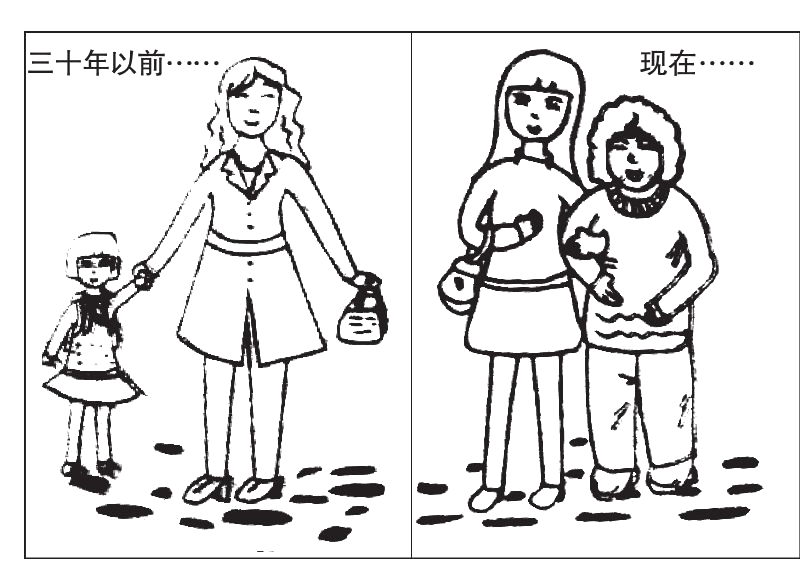
\includegraphics[width=0.56\linewidth]{picture/2014.png}
	\caption*{相携}
\end{figure}


%

\bta{2015}



\section{Use of English}

\noindent
\textbf{Directions:}\\
{Read the following text. Choose the best word (s) for each
	numbered blank and mark A, B, C or D on \textbf{ANSWER SHEET 1}. (10 points)}


\TiGanSpace


Though not biologically related, friends are as ``related'' as fourth
cousins, sharing about 1\% of genes. That is \cloze a
study, published from the University of California and Yale University in
the Proceedings of the National Academy of Sciences, has \cloze .

The study is a genome-wide analysis conducted \cloze 1932 unique
subjects which \cloze pairs of unrelated friends and unrelated
strangers. The same people were used in both \cloze.

While 1\% may seem \cloze , it is not so to a geneticist. As
co-author of the study James Fowler, professor of medical genetics at UC
San Diego, says, " Most people do not even \cloze their fourth
cousins but somehow manage to select as friends the people who
\cloze our kin."

The study \cloze found that the genes for smell were something
shared in friends but not genes for immunity. Why this similarity exists
in smell genes is difficult to explain, for now. \cloze , as the
team suggests, it draws us to similar environments but there is more
\cloze it. There could be many mechanisms working together that
\cloze us in choosing genetically similar friends \cloze
``functional kinship'' of being friends with \cloze !

One of the remarkable findings of the study was that the similar genes
seem to be evolving \cloze than other genes. Studying this could
help \cloze why human evolution picked pace in the last 30, 000
years, with social environment being a major \cloze factor.

The findings do not simply explain people's \cloze to befriend
those of similar \cloze backgrounds, say the researchers. Though
all the subjects were drawn from a population of European extraction,
care was taken to \cloze that all subjects, friends and strangers
were taken from the same population.


\newpage
\begin{enumerate}
	%\renewcommand{\labelenumi}{\arabic{enumi}.}
	% A(\Alph) a(\alph) I(\Roman) i(\roman) 1(\arabic)
	%设定全局标号series=example	%引用全局变量resume=example
	%[topsep=-0.3em,parsep=-0.3em,itemsep=-0.3em,partopsep=-0.3em]
	%可使用leftmargin调整列表环境左边的空白长度 [leftmargin=0em]
	\item

\fourchoices
{when}
{why}
{how}
{what}




\item


\fourchoices
{defended}
{concluded}
{withdrawn}
{advised}




\item


\fourchoices
{for}
{with}
{on}
{by}




\item


\fourchoices
{compared}
{sought}
{separated}
{connected}




\item


\fourchoices
{tests}
{objects}
{samples}
{examples}




\item

\fourchoices
{insignificant}
{unexpected}
{unreliable}
{incredible}



\item


\fourchoices
{visit}
{miss}
{seek}
{know}




\item


\fourchoices
{resemble}
{influence}
{favor}
{surpass}




\item


\fourchoices
{again}
{also}
{instead}
{thus}




\item

\fourchoices
{Meanwhile}
{Furthermore}
{Likewise}
{Perhaps}



\item


\fourchoices
{about}
{to}
{from}
{like}




\item


\fourchoices
{drive}
{observe}
{confuse}
{limit}




\item

\fourchoices
{according to}
{rather than}
{regardless of}
{along with}


\item


\fourchoices
{chances}
{responses}
{missions}
{benefits}




\item


\fourchoices
{later}
{slower}
{faster}
{earlier}




\item


\fourchoices
{forecast}
{remember}
{understand}
{express}




\item

\fourchoices
{unpredictable}
{contributory}
{controllable}
{disruptive}


\item

\fourchoices
{endeavor}
{decision}
{arrangement}
{tendency}



\item


\fourchoices
{political}
{religious}
{ethnic}
{economic}




\item


\fourchoices
{see}
{show}
{prove}
{tell}

\end{enumerate}

\vfil

\section{Reading Comprehension}


\noindent
\textbf{Part A}\\
\textbf{Directions:}\\
Read the following four texts. Answer the questions below each
	text by choosing A, B, C or
	D. Mark your answers on the \textbf{ANSWER SHEET 1}.
	(40 points)

\newpage
\subsection{Text 1}


King Juan Carlos of Spain once insisted ``kings don't abdicate, they die
in their sleep.'' But embarrassing scandals and the popularity of the
republican left in the recent Euro-elections have forced him to eat his
words and stand down. So, does the Spanish crisis suggest that monarchy
is seeing its last days? Does that mean the writing is on the wall for
all European royals, with their magnificent uniforms and majestic
lifestyles?

The Spanish case provides arguments both for and against monarchy. When
public opinion is particularly polarised, as it was following the end of
the Franco regime, monarchs can rise above ``mere'' politics and
``embody'' a spirit of national unity.

It is this apparent transcendence of politics that explains monarchs'
continuing popularity as heads of state. And so, the Middle East
excepted, Europe is the most monarch-infested region in the world, with
10 kingdoms (not counting Vatican City and Andorra). But unlike their
absolutist counterparts in the Gulf and Asia, most royal families have
survived because they allow voters to avoid the difficult search for a
non-controversial but respected public figure.

Even so, kings and queens undoubtedly have a downside. Symbolic of
national unity as they claim to be, their very history---and sometimes
the way they behave today---embodies outdated and indefensible
privileges and inequalities. At a time when Thomas Piketty and other
economists are warning of rising inequality and the increasing power of
inherited wealth, it is bizarre that wealthy aristocratic families
should still be the symbolic heart of modern democratic states.

The most successful monarchies strive to abandon or hide their old
aristocratic ways. Princes and princesses have day-jobs and ride
bicycles, not horses (or helicopters). Even so, these are wealthy
families who party with the international 1\%, and media intrusiveness
makes it increasingly difficult to maintain the right image.

While Europe's monarchies will no doubt be smart enough to survive for
some time to come, it is the British royals who have most to fear from
the Spanish example.

It is only the Queen who has preserved the monarchy's reputation with
her rather ordinary (if well-heeled) granny style. The danger will come
with Charles, who has both an expensive taste of lifestyle and a pretty
hierarchical view of the world. He has failed to understand that
monarchies have largely survived because they provide a service---as
non-controversial and non-political heads of state. Charles ought to
know that as English history shows, it is kings, not republicans, who
are the monarchy's worst enemies.


\begin{enumerate}[resume]
	%\renewcommand{\labelenumi}{\arabic{enumi}.}
	% A(\Alph) a(\alph) I(\Roman) i(\roman) 1(\arabic)
	%设定全局标号series=example	%引用全局变量resume=example
	%[topsep=-0.3em,parsep=-0.3em,itemsep=-0.3em,partopsep=-0.3em]
	%可使用leftmargin调整列表环境左边的空白长度 [leftmargin=0em]
	\item
 According to the first two Paragraphs, King Juan
	Carlosof Spain \lineread.


\fourchoices
{used to enjoy high public support}
{was unpopular among European royals}
{eased his relationship with his rivals}
{ended his reign in embarrassment}


\item
 Monarchs are kept as heads of state in Europe
mostly \lineread.


\fourchoices
{owing to their undoubted and respectable status}
{to achieve a balance between tradition and reality}
{to give voters more public figures to look up to}
{due to their everlasting political embodiment}



\item
Which of the following is shown to be odd, according to
Paragraph 4?


\fourchoices
{Aristocrats' excessive reliance on inherited wealth.}
{The role of the nobility in modern democracies.}
{The simple lifestyle of the aristocratic families.}
{The nobility's adherence to their privileges.}


\item
The British royals ``have most to fear'' because
Charles \lineread.


\fourchoices
{takes a tough line on political issues}
{fails to change his lifestyle as advised}
{takes republicans as his potential allies}
{fails to adapt himself to his future role}



\item
Which of the following is the best title of the text?


\fourchoices
{Carlos, Glory and Disgrace Combined}
{Charles, Anxious to Succeed to the Throne}
{Carlos, a Lesson for All European Monarchs}
{Charles, Slow to React to the Coming Threats}


\end{enumerate}


\newpage
\subsection{Text 2}


Just how much does the Constitution protect your digital data? The
Supreme Court will now consider whether police can search the contents
of a mobile phone without a warrant if the phone is on or around a
person during an arrest.

California has asked the justices to refrain from a sweeping ruling,
particularly one that upsets the old assumption that authorities may
search through the possessions of suspects at the time of their arrest.
It is hard, the state argues, for judges to assess the implications of
new and rapidly changing technologies.

The court would be recklessly modest if it followed California's advice.
Enough of the implications are discernable, even obvious, so that the
justices can and should provide updated guidelines to police, lawyers and
defendants.

They should start by discarding California's lame argument that
exploring the contents of a smartphone---a vast storehouse of digital
information---is similar to, say, going through a suspect's purse. The
court has ruled that police don't violate the Fourth Amendment when they
go through the wallet or pocketbook of an arrestee without a warrant.
But exploring one's smartphone is more like entering his or her home. A
smartphone may contain an arrestee's reading history, financial history,
medical history and comprehensive records of recent correspondence. The
development of ``cloud computing,'' meanwhile, has made that exploration
so much the easier.

Americans should take steps to protect their digital privacy. But
keeping sensitive information on these devices is increasingly a
requirement of normal life. Citizens still have a right to expect
private documents to remain private and protected by the Constitution's
prohibition on unreasonable searches.

As so often is the case, stating that principle doesn't ease the
challenge of line-drawing. In many cases, it would not be overly
burdensome for authorities to obtain a warrant to search through phone
contents. They could still invalidate Fourth Amendment protections when
facing severe, urgent circumstances, and they could take reasonable
measures to ensure that phone data are not erased or altered while
waiting for a warrant. The court, though, may want to allow room for
police to cite situations where they are entitled to more freedom.

But the justices should not swallow California's argument whole. New,
disruptive technology sometimes demands novel applications of the
Constitution's protections. Orin Kerr, a law professor, compares the
explosion and accessibility of digital information in the 21st century
with the establishment of automobile use as a virtual necessity of life
in the 20th: The justices had to specify novel rules for the new
personal domain of the passenger car then; they must sort out how the
Fourth Amendment applies to digital information now.


\begin{enumerate}[resume]
	%\renewcommand{\labelenumi}{\arabic{enumi}.}
	% A(\Alph) a(\alph) I(\Roman) i(\roman) 1(\arabic)
	%设定全局标号series=example	%引用全局变量resume=example
	%[topsep=-0.3em,parsep=-0.3em,itemsep=-0.3em,partopsep=-0.3em]
	%可使用leftmargin调整列表环境左边的空白长度 [leftmargin=0em]
	\item
The Supreme Court will work out whether, during an arrest,
it is legitimate to \lineread.


\fourchoices
{prevent suspects from deleting their phone contents}
{search for suspects' mobile phones without a warrant}
{check suspects' phone contents without being authorized}
{prohibit suspects from using their mobile phones}


\item
The author's attitude toward California's argument is one
of \lineread.


\fourchoices
{disapproval}
{indifference}
{tolerance}
{cautiousness}



\item
The author believes that exploring one's phone contents is
comparable to \lineread.


\fourchoices
{getting into one's residence}
{handling one's historical records}
{scanning one's correspondences}
{going through one's wallet}



\item
 In Paragraph 5 and 6, the author shows his concern
that \lineread.


\fourchoices
{principles are hard to be clearly expressed}
{the court is giving police less room for action}
{citizens' privacy is not effectively protected}
{phones are used to store sensitive information}


\item
Orin Kerr's comparison is quoted to indicate
that \lineread.


\fourchoices
{the Constitution should be implemented flexibly}
{new technology requires reinterpretation of the Constitution}
{California's argument violates principles of the Constitution}
{principles of the Constitution should never be altered}


\end{enumerate}



\newpage
\subsection{Text 3}


The journal Science is adding an extra round of statistical checks to
its peer-review process, editor-in-chief Marcia McNutt announced today.
The policy follows similar efforts from other journals, after widespread
concern that basic mistakes in data analysis are contributing to the
irreproducibility of many published research findings.

``Readers must have confidence in the conclusions published in our
journal,'' writes McNutt in an editorial. Working with the American
Statistical Association, the journal has appointed seven experts to a
statistic board of reviewing editors (SBoRE). Manuscript will be
\uline{flagged up} for additional scrutiny by the journal's internal
editors, or by its existing Board of Reviewing Editors or by outside
peer reviewers. The SBoRE panel will then find external statisticians to
review these manuscripts.

Asked whether any particular papers had impelled the change, McNutt
said: ``The creation of the `statistics board' was motivated by concerns
broadly with the application of statistics and data analysis in
scientific research and is part of Science's overall drive to increase
reproducibility in the research we publish.''

Giovanni Parmigiani, a biostatistician at the Harvard School of Public
Health, a member of the SBoRE group, says he expects the board to ``play
primarily an advisory role.'' He agreed to join because he ``found the
foresight behind the establishment of the SBoRE to be novel, unique and
likely to have a lasting impact. This impact will not only be through
the publications in Science itself, but hopefully through a larger group
of publishing places that may want to model their approach
after \emph{Science}.''

John Ioannidis, a physician who studies research methodology, says that
the policy is ``a most welcome step forward'' and ``long overdue.''
``Most journals are weak in statistical review, and this damages the
quality of what they publish. I think that, for the majority of
scientific papers nowadays, statistical review is more essential than
expert review,'' he says. But he noted that biomedical journals such as
\emph{Annals of Internal Medicine, the Journal of the American Medical
Association} and \emph{The Lancet} pay strong attention to statistical review.

Professional scientists are expected to know how to analyze data, but
statistical errors are alarmingly common in published research,
according to David Vaux, a cell biologist. Researchers should improve
their standards, he wrote in 2012, but journals should also take a
tougher line, ``engaging reviewers who are statistically literate and
editors who can verify the process.'' Vaux says that Science's idea to
pass some papers to statisticians ``has some merit, but a weakness is
that it relies on the board of reviewing editors to identify `the papers
that need scrutiny' in the first place''.


\begin{enumerate}[resume]
	%\renewcommand{\labelenumi}{\arabic{enumi}.}
	% A(\Alph) a(\alph) I(\Roman) i(\roman) 1(\arabic)
	%设定全局标号series=example	%引用全局变量resume=example
	%[topsep=-0.3em,parsep=-0.3em,itemsep=-0.3em,partopsep=-0.3em]
	%可使用leftmargin调整列表环境左边的空白长度 [leftmargin=0em]
	\item
It can be learned from Paragraph 1 that \lineread.


\fourchoices
{\emph{Science} intends to simplify its peer-review process}
{journals are strengthening their statistical checks}
{few journals are blamed for mistakes in data analysis}
{lack of data analysis is common in research projects}


\item
The phrase ``flagged up'' (Para. 2) is the closest in
meaning to \lineread.



\fourchoices
{found}
{marked}
{revised}
{stored}




\item
Giovanni Parmigiani believes that the establishment of the
SBoRE may \lineread.


\fourchoices
{pose a threat to all its peers}
{meet with strong opposition}
{increase \emph{Science}'s circulation}
{set an example for other journals}



\item
 David Vaux holds that what \emph{Science} is doing
	now \lineread.


\fourchoices
{adds to researchers' workload}
{diminishes the role of reviewers}
{has room for further improvement}
{is to fail in the foreseeable future}



\item
Which of the following is the best title of the text?


\fourchoices
{\emph{Science} Joins Push to Screen Statistics in Papers}
{Professional Statisticians Deserve More Respect}
{Data Analysis Finds Its Way onto Editors' Desks}
{Statisticians Are Coming Back with \emph{Science}}


\end{enumerate}


\newpage
\subsection{Text 4}


Two years ago, Rupert Murdoch's daughter, Elisabeth, spoke of the
``unsettling dearth of integrity across so many of our institutions.''
Integrity had collapsed, she argued, because of a collective acceptance
that the only ``sorting mechanism'' in society should be profit and the
market. But ``it's us, human beings, we the people who create the
society we want, not profit''.

Driving her point home, she continued: ``It's increasingly apparent that
the absence of purpose, of a moral language within government, media or
business could become one of the most dangerous goals for capitalism and
freedom.'' This same absence of moral purpose was wounding companies
such as News International, she thought, making it more likely that it
would lose its way as it had with widespread illegal telephone hacking.

As the hacking trial concludes---finding guilty one ex-editor of
the \emph{News of the World}, Andy Coulson, for conspiring to hack
phones, and finding his predecessor, Rebekah Brooks, innocent of the
same charge---the wider issue of dearth of integrity still
stands. Journalists are known to have hacked the phones of up to 5, 500
people. This is hacking on an industrial scale, as was acknowledged by
Glenn Mulcaire, the man hired by the \emph{News of the World} in 2001 to
be the point person for phone hacking. Others await trial. This long
story still unfolds.

In many respects, the dearth of moral purpose frames not only the fact
of such widespread phone hacking but the terms on which the trial took
place. One of the astonishing revelations was how little Rebekah Brooks
knew of what went on in her newsroom, how little she thought to ask and
the fact that she never inquired how the stories arrived. The core of
her successful defence was that she knew nothing.

In today's world, it has become normal that well-paid executives should
not be accountable for what happens in the organizations that they run.
Perhaps we should not be so surprised. For a generation, the collective
doctrine has been that the sorting mechanism of society should be
profit. The words that have mattered are efficiency, flexibility,
shareholder value, business--friendly, wealth generation, sales, impact
and, in newspapers, circulation. Words degraded to the margin have been
justice, fairness, tolerance, proportionality and accountability.

The purpose of editing the \emph{News of the World} was not to promote reader
understanding, to be fair in what was written or to betray any common
humanity. It was to ruin lives in the quest for circulation and impact.
Ms Brooks may or may not have had suspicions about how her journalists
got their stories, but she asked no questions, gave no
instructions---nor received traceable, recorded answers.


\begin{enumerate}[resume]
	%\renewcommand{\labelenumi}{\arabic{enumi}.}
	% A(\Alph) a(\alph) I(\Roman) i(\roman) 1(\arabic)
	%设定全局标号series=example	%引用全局变量resume=example
	%[topsep=-0.3em,parsep=-0.3em,itemsep=-0.3em,partopsep=-0.3em]
	%可使用leftmargin调整列表环境左边的空白长度 [leftmargin=0em]
	\item
According to the first two paragraphs, Elisabeth was upset
by \lineread.


\fourchoices
{the consequences of the current sorting mechanism}
{companies' financial loss due to immoral practices}
{governmental ineffectiveness on moral issues}
{the wide misuse of integrity among institutions}


\item
It can be inferred from Paragraph 3 that \lineread.

\fourchoices
{Glem Mulcaire may deny phone hacking as a crime}
{more journalists may be found guilty of phone hacking}
{Andy Coulson should be held innocent of the charge}
{phone hacking will be accepted on certain occasions}


\item
The author believes the Rebekah Books's
defence \lineread.


\fourchoices
{revealed a cunning personality}
{centered on trivial issues}
{was hardly convincing}
{was part of a conspiracy}



\item
The author holds that the current collective doctrine
shows \lineread.


\fourchoices
{generally distorted values}
{unfair wealth distribution}
{a marginalized lifestyle}
{a rigid moral code}



\item
Which of the following is suggested in the last paragraph?


\fourchoices
{The quality of writing is of primary importance.}
{Journalists need stricter industrial regulations.}
{Moral awareness matters in editing a newspaper.}
{Common humanity is central to news reporting.}



\end{enumerate}

\newpage
\noindent
\textbf{Part B}\\
\textbf{Directions:}\\
In the following text, some sentences have been removed. For
	Questions 41-45, choose the most suitable one from the fist A-G to fit
	into each of the numbered blanks. There are two extra choices, which do
	not fit in any of the gaps. Mark your answers on \textbf{ANSWER SHEET}. (10 points)


\TiGanSpace

How does your reading proceed? Clearly you try to comprehend, in the
sense of identifying meanings for individual words and working out
relationships between them, drawing on your implicit knowledge of
English grammar. \linefill. You begin to infer a context for
the text, for instance, by making decisions about what kind of speech
event is involved. Who is making the utterance, to whom, when and where.

The ways of reading indicated here are without doubt kinds of
comprehension. But they show comprehension to consist not just of
passive assimilation but of active engagement in inference and
problem-solving. You infer information you feel the writer has invited
you to grasp by presenting you with specific evidence and clues. \linefill.

Conceived in this way, comprehension will not follow exactly the same
track for each reader. What is in question is not the retrieval of an
absolute, fixed or ``true'' meaning that can be read off and checked for
accuracy, or some timeless relation of the text to the world. \linefill.

Such background material inevitably reflects who we are. \linefill. This doesn't, however, make interpretation merely
relative or even pointless. Precisely because readers from different
historical periods, places and social experiences produce different but
overlapping readings of the same words on the page---including for
texts that engage with fundamental human concerns---debates about
texts can play an important role in social discussion of beliefs and
values.

How we read a given text also depends to some extent on our particular
interest in reading it. \linefill. Such dimensions of reading
suggest---as others introduced later in the book will also
do---that we bring an implicit (often unacknowledged) agenda to any
act of reading. It doesn't then necessarily follow that one kind of
reading is fuller, more advanced or more worthwhile than another.
Ideally, different kinds of reading inform each other, and act as useful
reference points for and counterbalances to one another. Together, they
make up the reading component of your overall literacy, or relationship
to your surrounding textual environment.

\begin{listmatch}
	%\renewcommand{\labelenumi}{\arabic{enumi}.}
	% A(\Alph) a(\alph) I(\Roman) i(\roman) 1(\arabic)
	%设定全局标号series=example	%引用全局变量resume=example
	%[topsep=-0.3em,parsep=-0.3em,itemsep=-0.3em,partopsep=-0.3em]
	%可使用leftmargin调整列表环境左边的空白长度 [leftmargin=0em]
	\item
 Are we studying that text and trying to respond in a
way that fulfils the requirement of a given course? Reading it simply
for pleasure? Skimming it for information? Ways of reading on a train or
in bed are likely to differ considerably from reading in a seminar
room.

\item 
Factors such as the place and period in which we are
reading, our gender, ethnicity, age and social class will encourage us
towards certain interpretations but at the same time obscure or even
close off others.

\item 
 If you are unfamiliar with words or idioms, you guess
at their meaning, using clues presented in the context. On the
assumption that they will become relevant later, you make a mental note
of discourse entities as well as possible links between them.


\item 
In effect, you try to reconstruct the likely meanings or
effects that any given sentence, image or reference might have had:
These might be the ones the author intended.


\item 
You make further inferences, for instance, about how the
text may be significant to you, or about its validity---inferences that
form the basis of a personal response for which the author will
inevitably be far less responsible.

\item 
In plays, novels and narrative poems, characters speak
as constructs created by the author, not necessarily as mouthpieces for
the author's own thoughts.


\item 
Rather, we ascribe meanings to texts on the basis of
interaction between what we might call textual and contextual material:
between kinds of organization or patterning we perceive in a text's
formal structures (so especially its language structures) and various
kinds of background, social knowledge, belief and attitude that we bring
to the text.

\end{listmatch}


\newpage

\noindent
\textbf{Part C}\\
\textbf{Directions:}\\
Read the following text carefully and then translate the
	underlined segments into Chinese. Your translation should be written
	neatly on the \textbf{ANSWER SHEET}. (10 points)


\TiGanSpace

Within the span of a hundred years, in the seventeenth and early
eighteenth centuries, a tide of emigration---one of the great folk
wanderings of history---swept from Europe to America.
\transnum \uline{This movement, driven by powerful and diverse
	motivations, built a nation out of a wilderness and, by its nature,
	shaped the character and destiny of an uncharted continent}.

\transnum \uline{The United States is the product of two principal
	forces---the immigration of European peoples with their varied ideas,
	customs, and national characteristics and the impact of a new country
	which modified these traits}. Of necessity, colonial America was a
projection of Europe. Across the Atlantic came successive groups of
Englishmen, Frenchmen, Germans, Scots, Irishmen, Dutchmen, Swedes, and
many others who attempted to transplant their habits and traditions to
the new world. \transnum \uline{But, the force of geographic conditions
	peculiar to America, the interplay of the varied national groups upon
	one another, and the sheer difficulty of maintaining old-world ways in a
	raw, new continent caused significant changes}. These changes were
gradual and at first scarcely visible. But the result was a new social
pattern which, although it resembled European society in many ways, had
a character that was distinctly American.

\transnum \uline{The first shiploads of immigrants bound for the
	territory which is now the United States crossed the Atlantic more than
	a hundred years after the 15 th-and-16 th-century explorations of North
	America}. In the meantime, thriving Spanish colonies had been established
in

Mexico, the West Indies, and South America. These travelers to North
America came in small, unmercifully overcrowded craft. During their six-
to twelve-week voyage, they survived on barely enough food allotted to
them. Many of the ships were lost in storms, many passengers died of
disease, and infants rarely survived the journey. Sometimes storms blew
the vessels far off their course, and often calm brought unbearably long
delay.

To the anxious travelers the sight of the American shore brought almost
inexpressible relief. Said one recorder of events, ``The air at twelve
leagues' distance smelt as sweet as a new-blown garden.'' The colonists'
first glimpse of the new land was a sight of dense woods.
\transnum \uline{The virgin forest with its richness and variety of trees
	was a real treasure-house which extended from Maine all the way down to
	Georgia}. Here was abundant fuel and lumber. Here was the raw material
of houses and furniture, ships and potash, dyes and naval stores.



\newpage

\section{Writing}


\noindent
\textbf{Part A}\\
\textbf{51. Directions:}

You are going to host a club reading session. Write an email of about
100 words recommending a book to the club members.

You should state reasons for your recommendation.

You should write neatly on the ANSWER SHEET.

\textbf{Do not} sign your own name at the end of the letter. Use Li Ming
instead.

\textbf{Do not} write the address. (10 points)


\vspace{2em}

\noindent
\textbf{Part B}\\
\textbf{52. Directions:}

Write an essay of 160-200 words based on the following drawing. In your
essay, you should
\begin{listwrite}
	%\renewcommand{\labelenumi}{\arabic{enumi}.}
	% A(\Alph) a(\alph) I(\Roman) i(\roman) 1(\arabic)
	%设定全局标号series=example	%引用全局变量resume=example
	%[topsep=-0.3em,parsep=-0.3em,itemsep=-0.3em,partopsep=-0.3em]
	%可使用leftmargin调整列表环境左边的空白长度 [leftmargin=0em]
	\item
 describe the drawing briefly
\item 
 explain its intended meaning, and
\item 
 give your comments.
	
\end{listwrite}

You should write neatly on the ANSWER SHEET. (20 points)

\begin{figure}[h!]
	\centering
	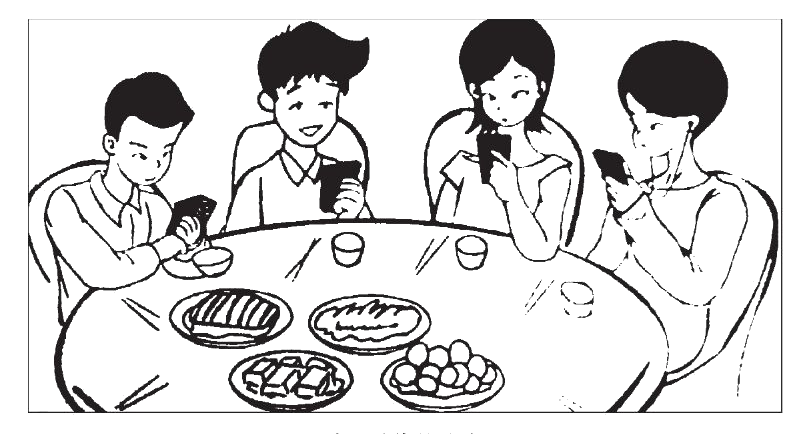
\includegraphics[width=0.58\linewidth]{picture/2015.png}
	\caption*{手机时代的聚会}
\end{figure}

%
\bta{2016}



\section{Use of English}

\noindent
\textbf{ Directions:}\\
Read the following text. Choose the best word (s) for each
	numbered blank and mark A, B, C or D on the \textbf{ANSWER SHEET}. (10 points)


\TiGanSpace

In Cambodia, the choice of a spouse is a complex one for the young
male. It may involve not only his parents and his
friends, \cloze those of the young women, but also a
matchmaker. A young man can \cloze a likely spouse on his own
and them ask his parents to \cloze the marriage negotiations, or
the young man's parents may make the choice of a spouse, giving the
child little to say in the selection. \cloze , a girl may veto
the spouse her parents have chosen. \cloze a spouse has been
selected, each family investigates the other to make sure its child is
marrying \cloze a good family.

The traditional wedding is a long and colorful affair. Formerly it
lasted three days, \cloze by the 1980s it more commonly lasted a
day and a half. Buddhist priests offer a short sermon and \cloze
prayers of blessing. Parts of the ceremony involve ritual hair
cutting, \cloze cotton threads soaked in holy water around the
bride's and groom's wrists , and \cloze a candle around a circle
of happily married and respected couples to bless the \cloze
. Newlyweds traditionally move in with the wife's parents and may
\cloze with them up to a year, \cloze they can build a
flew house nearby.

Divorce is legal and easy to \cloze , but not common. Divorced
persons are \cloze with some disapproval. Each spouse retains
\cloze property he or she \cloze into the marriage, and
jointly acquired property is \cloze equally. Divorced persons
may remarry, but a gender prejudice \cloze up. The divorced
male doesn't have a waiting period before he can remarry \cloze
the woman must wait the months.


\newpage

\begin{enumerate}
	%\renewcommand{\labelenumi}{\arabic{enumi}.}
	% A(\Alph) a(\alph) I(\Roman) i(\roman) 1(\arabic)
	%设定全局标号series=example	%引用全局变量resume=example
	%[topsep=-0.3em,parsep=-0.3em,itemsep=-0.3em,partopsep=-0.3em]
	%可使用leftmargin调整列表环境左边的空白长度 [leftmargin=0em]
	\item

\fourchoices
{by way of}
{as well as}
{on behalf of}
{with regard to}


\item

\fourchoices
{adapt to}
{provide for}
{compete with}
{decide on}



\item


\fourchoices
{close}
{renew}
{arrange}
{postpone}




\item


\fourchoices
{In theory}
{Above all}
{In time}
{For example}





\item


\fourchoices
{Although}
{Lest}
{After}
{Unless}




\item


\fourchoices
{into}
{within}
{from}
{through}




\item

\fourchoices
{since}
{or}
{but}
{so}



\item


\fourchoices
{test}
{copy}
{recite}
{create}




\item


\fourchoices
{folding}
{piling}
{wrapping}
{tying}




\item


\fourchoices
{lighting}
{passing}
{hiding}
{serving}




\item

\fourchoices
{meeting}
{association}
{collection}
{union}




\item


\fourchoices
{grow}
{part}
{deal}
{live}




\item


\fourchoices
{whereas}
{until}
{for}
{if}




\item


\fourchoices
{obtain}
{follow}
{challenge}
{avoid}




\item

\fourchoices
{isolated}
{persuaded}
{viewed}
{exposed}



\item

\fourchoices
{wherever}
{however}
{whenever}
{whatever}


\item


\fourchoices
{changed}
{brought}
{shaped}
{pushed}




\item

\fourchoices
{divided}
{invested}
{donated}
{withdrawn}


\item


\fourchoices
{clears}
{warms}
{shows}
{breaks}




\item


\fourchoices
{while}
{so what}
{once}
{in that}


\end{enumerate}

\vfil

\section{Reading Comprehension}


\noindent
\textbf{Part A}\\
\textbf{ Directions:}\\
 Read the following four texts. Answer the questions below
	each text by choosing A, B, C or
	D. Mark your answers on the \textbf{ANSWER SHEET}. (40 points)

\newpage
\subsection{Text 1}


France, which prides itself as the global innovator of fashion,
has decided its fashion industry has lost an absolute right to define
physical beauty for woman. Its lawmakers gave preliminary approval last
week to a law that would make it a crime to employ ultra-thin models on
runways. The parliament also agreed to ban websites that ``incite
excessive thinness'' by promoting extreme dieting.

Such measures have a couple of uplifting motives. They suggest
beauty should not be defined by looks that end up \uline{impinging on} health.
That's a start. And the ban on ultra-thin models seems to go beyond
protecting models from starving themselves to death---as some have
done. It tells the fashion industry that it must take responsibility for
the signal it sends women, especially teenage girls, about the social
tape--measure they must use to determine their individual worth.

The bans, if fully enforced , would suggest to woman (and many men) that they should not let others be arbiters of their beauty. And
perhaps faintly, they hint that people should look to intangible
qualities like character and intellect rather than dieting their way to
size zero or wasp-waist physiques.

The French measures, however, rely too much on severe punishment to
change a culture that still regards beauty as skin-deep---and
bone-showing. Under the law, using a fashion model that does not meet
a government-defined index of body mass could result in a \$85, 000 fine
and six months in prison.

The fashion industry knows it has an inherent problem in focusing on
material adornment and idealized body types. In Denmark, the United
States, and a few other countries, it is trying to set voluntary
standard for models and fashion images that rely more on peer pressure
for enforcement.

In contrast to France's actions, Denmark's fashion industry agreed last
month on rules and sanctions regarding the age, health, and other
characteristics of models. The newly revised Danish Fashion Ethical
Charter clearly states: ``We are aware of and take responsibility for
the impact the fashion industry has on body ideals, especially on young
people.'' The charter's main tool of enforcement is to deny access for
designers and modeling agencies to Copenhagen Fashion Week (CFW), which is
run by the Danish Fashion Institute. But in general it relies on a
name-and-shame method of compliance.

Relying on ethical persuasion rather than law to address the misuse of
body ideals may be the best step. Even better would be to help elevate
notions of beauty beyond the material standards of a particular
industry.


\begin{enumerate}[resume]
	%\renewcommand{\labelenumi}{\arabic{enumi}.}
	% A(\Alph) a(\alph) I(\Roman) i(\roman) 1(\arabic)
	%设定全局标号series=example	%引用全局变量resume=example
	%[topsep=-0.3em,parsep=-0.3em,itemsep=-0.3em,partopsep=-0.3em]
	%可使用leftmargin调整列表环境左边的空白长度 [leftmargin=0em]
	\item
According to the first paragraph, what would happen in
France?


\fourchoices
{New runways would be constructed}
{Physical beauty would be redefined}
{Websites about dieting would thrive}
{The fashion industry would decline}



\item
The phrase ``impinging on'' (Line 2 Para. 2) is closest in
meaning to \lineread.


\fourchoices
{heightening the value of}
{indicating the state of}
{losing faith in}
{doing harm to}


\item
Which of the following is true of the fashion
industry?


\fourchoices
{New standards are being set in Denmark}
{The French measures have already failed}
{Models are no longer under peer pressure}
{Its inherent problems are getting worse}



\item
A designer is most likely to be rejected by CFW for \lineread.


\fourchoices
{pursuing perfect physical conditions}
{caring too much about models' character}
{showing little concern for health factors}
{setting a high age threshold for models}


\item
Which of the following may be the best title of the
text?


\fourchoices
{A Challenge to the Fashion Industry's Body Ideals}
{A Dilemma for the Starving Models in France}
{Just Another Round of Struggle for Beauty}
{The Great Threats to the Fashion Industry}


\end{enumerate}


\newpage
\subsection{Text 2}


For the first time in the history more people live in towns than in the
country. In Britain this has had a curious result. While polls show
Britons rate ``the countryside'' alongside the royal family.
Shakespeare and the National Health Service (NHS) as what makes them
proudest of their country, this has limited political support.

A century ago Octavia Hill launched the National Trust not to rescue
stylish houses but to save ``the beauty of natural places for everyone
forever''. It was specifically to provide city dwellers with spaces for
leisure where they could experience ``a refreshing air''. Hill's
pressure later led to the creation of national parks and green belts.
They don't make countryside any more, and every year concrete consumes
more of it. It needs constant guardianship.

At the next election none of the big parties seem likely to endorse
this sentiment. The Conservatives' planning reform explicitly gives
rural development priority over conservation, even authorizing
``off--plan'' building where local people might object. The concept of
sustainable development has been defined as profitable. Labour likewise
wants to discontinue local planning where councils oppose development.
The Liberal Democrats are silent. Only Ukip, sensing its chance, has
sided with those pleading for a more considered approach to using green
land. Its Campaign to Protect Rural England struck terror into many
local Conservative parties.

The sensible place to build new houses, factories and offices is
where people are, in cities and towns where infrastructure is in
place. The London agents Stirling Ackroyd recently identified enough
sites for half a million houses in the London area alone, with no
intrusion on green belts. What is true of London is even truer of the
provinces.

The idea that ``housing crisis'' equals ``concreted meadows'' is pure
lobby talk. The issue is not the need for more houses but, as always,
where to put them. Under lobby pressure, George Osborne favours rural
new-build against urban renovation and renewal. He favours out-of-town
shopping sites against high streets. This is not a free market but a
biased one. Rural towns and villages have grown and will always grow.
They do so best where building sticks to their edges and respects their
character. We do not ruin urban conservation areas. Why ruin rural
ones?

Development should be planned, not let rip, After the
Netherlands, Britain is Europe's most crowded country. Half a century
of town and country planning has enabled it to retain an enviable rural
coherence, while still permitting low-density urban living. There is
no doubt of the alternative---the corrupted landscapes of southern
Portugal, Spain or Ireland. Avoiding this rather than promoting it
should unite the left and right of the political spectrum.


\begin{enumerate}[resume]
	%\renewcommand{\labelenumi}{\arabic{enumi}.}
	% A(\Alph) a(\alph) I(\Roman) i(\roman) 1(\arabic)
	%设定全局标号series=example	%引用全局变量resume=example
	%[topsep=-0.3em,parsep=-0.3em,itemsep=-0.3em,partopsep=-0.3em]
	%可使用leftmargin调整列表环境左边的空白长度 [leftmargin=0em]
	\item
 Britain's public sentiment about the countryside \lineread.


\fourchoices
{didn't start till the Shakespearean age}
{has brought much benefit to the NHS}
{is fully backed by the royal family}
{is not well reflected in politics}




\item
According to Paragraph 2, the achievements of the National
Trust are now being \lineread.


\fourchoices
{gradually destroyed}
{effectively reinforced}
{largely overshadowed}
{properly protected}



\item
Which of the following can be inferred from Paragraph 3?


\fourchoices
{Labour is under attack for opposing development}
{The Conservatives may abandon ``off-plan'' building}
{The Liberal Democrats are losing political influence}
{Ukip may gain from its support for rural conservation}


\item
The author holds that George Osbornes's preference \lineread.


\fourchoices
{highlights his firm stand against lobby pressure}
{shows his disregard for the character of rural areas}
{stresses the necessity of easing the housing crisis}
{reveals a strong prejudice against urban areas}



\item
 In the last paragraph the author shows his appreciation of \lineread.


\fourchoices
{the size of population in Britain}
{the political life in today's Britain}
{the enviable urban lifestyle in Britain}
{the town-and-country planning in Britain}



\end{enumerate}


\newpage
\subsection{Text 3}


``There is one and only one social responsibility of business,''
Wrote Milton Friedman, a Nobel Prize-winning economist, ``That is, to
use its resources and engage in activities designed to increase its
profits.'' But even if you accept Friedman's premise and regard
corporate social responsibility (CSR) policies as a waste of
shareholders's money, things may not be absolutely clear-cut. New
research suggests that CSR may create monetary value for companies---at least when they are prosecuted for corruption.

The largest firms in America and Britain together spend more than
\$15 billion a year on CSR, according to an estimate by EPG, a
consulting firm. This could add value to their businesses in three
ways. First, consumers may take CSR spending as a ``signal'' that a
company's products are of high quality. Second, customers may be
willing to buy a company's products as an indirect may to donate to the
good causes it helps. And third, through a more diffuse ``halo
effect'' whereby its good deeds earn it greater consideration from
consumers and others.

Previous studies on CSR have had trouble differentiating these effects
because consumers can be affected by all three. A recent study attempts
to separate them by looking at bribery prosecutions under American's
Foreign Corrupt Practices Act (FCPA). It argues that since prosecutors
do not consume a company's products as part of their
investigations, they could be influenced only by the halo effect.

The study found that, among prosecuted firms, those with the most
comprehensive CSR programmes tended to get \uline{more lenient} penalties.
Their analysis ruled out the possibility that it was firm's political
influence, rather than their CSR stand, that accounted for the
leniency: Companies that contributed more to political campaigns did not
receive lower fines.

In all, the study concludes that whereas prosecutors should only
evaluate a case based on its merits, they do seem to be influenced by a
company's record in CSR. ``We estimate that either eliminating a
substantial labour-rights concern, such as child labour, or increasing
corporate giving by about 20\% result in fines that generally are 40\%
lower than the typical punishment for bribing foreign officials,'' says
one researcher.

Researchers admit that their study does not answer the question of
how much businesses ought to spend on CSR. Nor does it reveal how much
companies are banking on the halo effect, rather than the other
possible benefits, when they decide their do-gooding policies. But at
least they have demonstrated that when companies get into trouble with
the law, evidence of good character can win them a less costly
punishment.


\begin{enumerate}[resume]
	%\renewcommand{\labelenumi}{\arabic{enumi}.}
	% A(\Alph) a(\alph) I(\Roman) i(\roman) 1(\arabic)
	%设定全局标号series=example	%引用全局变量resume=example
	%[topsep=-0.3em,parsep=-0.3em,itemsep=-0.3em,partopsep=-0.3em]
	%可使用leftmargin调整列表环境左边的空白长度 [leftmargin=0em]
	\item
The author views Milton Friedman's statement about CSR
with \lineread.


\fourchoices
{tolerance}
{skepticism}
{uncertainty}
{approval}



\item
According to Paragraph 2, CSR helps a company by \lineread.


\fourchoices
{winning trust from consumers}
{guarding it against malpractices}
{protecting it from being defamed}
{raising the quality of its products}


\item
The expression ``more lenient'' (line 2, Para. 4) is
closest in meaning to \lineread.


\fourchoices
{more effective}
{less controversial}
{less severe}
{more lasting}


\item
 When prosecutors evaluate a case, a company's CSR
record \lineread.


\fourchoices
{has an impact on their decision}
{comes across as reliable evidence}
{increases the chance of being penalized}
{constitutes part of the investigation}


\item
Which of the following is true of CSR according to the
last paragraph?


\fourchoices
{Its negative effects on businesses are often overlooked}
{The necessary amount of companies spending on it is unknown}
{Companies' financial capacity for it has been overestimated}
{It has brought much benefit to the banking industry}


\end{enumerate}



\newpage
\subsection{Text 4}


There will eventually come a day when \emph{The New York Times} ceases to
publish stories on newsprint. Exactly when that day will be is a matter
of debate. ''Sometime in the future,'' the paper's publisher said back
in 2010.

Nostalgia for ink on paper and the rustle of pages aside, there's
plenty of incentive to ditch print. The infrastructure required to make
a physical newspaper---printing presses, delivery trucks---isn't just
expensive; it's excessive at a time when online-only competitors
don't have the same set of financial constraints. Readers are migrating
away from print anyway. And though print ad sales still dwarf their
online and mobile counterparts, revenue from print is still declining.

Overhead may be high and circulation lower, but rushing to
eliminate its print edition would be a mistake, says BuzzFeed CEO Jonah
Peretti.

Peretti says the \emph{Times} shouldn't waste time getting out of the
print business, but only if they go about doing it the right way.
``Figuring out a way to accelerate that transition would make sense for
them,'' he said, ``but if you discontinue it, you're going to have
your most loyal customers really upset with you.''

Sometimes that's worth making a change anyway. Peretti gives the
example of Netflix discontinuing its DVD--mailing service to focus on
streaming. ``It was seen as blunder,'' he said. The move turned out
to be foresighted. And if Peretti were in charge at the \emph{Times}? ``I
wouldn't pick a year to end print,'' he said. ``I would raise prices
and make it into more of a legacy product.''

The most loyal customers would still get the product they favor, the
idea goes, and they'd feel like they were helping sustain the quality
of something they believe in. ``So if you're overpaying for print, you
could feel like you were helping,'' Peretti said. ``Then increase it
at a higher rate each year and essentially try to generate additional
revenue.'' In other words, if you're going to make a print product,
make it for the people who are already obsessed with it. Which may be
what the Times is doing already. Getting the print edition seven days a
week costs nearly \$500 a year---more than twice as much as a digital--only subscription.

``It's a really hard thing to do and it's a tremendous luxury that
BuzzFeed doesn't have a legacy business,'' Peretti remarked. ``But
we're going to have questions like that where we have things we're doing
that don't make sense when the market changes and the world changes. In
those situations, it's better to be more aggressive than less
aggressive.''


\begin{enumerate}[resume]
	%\renewcommand{\labelenumi}{\arabic{enumi}.}
	% A(\Alph) a(\alph) I(\Roman) i(\roman) 1(\arabic)
	%设定全局标号series=example	%引用全局变量resume=example
	%[topsep=-0.3em,parsep=-0.3em,itemsep=-0.3em,partopsep=-0.3em]
	%可使用leftmargin调整列表环境左边的空白长度 [leftmargin=0em]
	\item
\emph{The New York Times} is considering ending its print
edition partly due to \lineread.


\fourchoices
{the high cost of operation}
{the pressure from its investors}
{the complaints from its readers}
{the increasing online ad sales}


\item
Peretti suggests that , in face of the present
situation, the \emph{Times} should \lineread.


\fourchoices
{seek new sources of readership}
{end the print edition for good}
{aim for efficient management}
{make strategic adjustments}

\item
 It can be inferred from Paragraphs 5 and 6 that a ``legacy
product'' \lineread.


\fourchoices
{helps restore the glory of former times}
{is meant for the most loyal customers}
{will have the cost of printing reduced}
{expands the popularity of the paper}



\item
Peretti believes that, in a changing world, \lineread.


\fourchoices
{legacy businesses are becoming outdated}
{cautiousness facilitates problem-solving}
{aggressiveness better meets challenges}
{traditional luxuries can stay unaffected}



\item
which of the following would be the best title of the
text?


\fourchoices
{Shift to Online Newspapers All at Once}
{Cherish the Newspapers Still in Your Hand}
{Make Your Print Newspapers a Luxury Good}
{Keep Your Newspapers Forever in Fashion}




\end{enumerate}

\newpage
\noindent
\textbf{Part B}\\
\textbf{ Directions:}\\
 Read the following text and answer the questions by choosing
	the most suitable subheading from the list A-G for each of the numbered
	paragraphs (41-45). There are two extra subheadings. Mark your answers
	on the \textbf{ANSER SHEET}. (10 point)

\begin{listmatch}
	%\renewcommand{\labelenumi}{\arabic{enumi}.}
	% A(\Alph) a(\alph) I(\Roman) i(\roman) 1(\arabic)
	%设定全局标号series=example	%引用全局变量resume=example
	%[topsep=-0.3em,parsep=-0.3em,itemsep=-0.3em,partopsep=-0.3em]
	%可使用leftmargin调整列表环境左边的空白长度 [leftmargin=0em]
	\item
Create a new image of yourself


\item 
 Decide if the time is right


\item 
 Have confidence in yourself


\item 
 Understand the context


\item 
 Work with professionals


\item 
 Make it efficient


\item 
 Know your goals
\end{listmatch}

No matter how formal or informal the work environment, the way you
present yourself has an impact. This is especially true in the first
impressions. According to research from Princeton University , people
assess your competence, trustworthiness, and likeability in just a
tenth of a second, solely based on the way you look.

The difference between today's workplace and the ``dress for
success'' era is that the range of options is so much broader. Norms
have evolved and fragmented. In some settings, red sneakers or dress
T-shirts can convey status; in others not so much. Plus, whatever
image we present is magnified by social-media services like LinkedIn.
Chances are, your headshots are seen much more often now than a decade
or two ago. Millennials, it seems, face the paradox of being the
least formal generation yet the most conscious of style and personal
branding. It can be confusing.

So how do we navigate this? How do we know when to invest in an
upgrade? And what's the best way to pull off one than enhances our
goals? Here are some tips:

\linefill.

As an executive coach, I've seen image upgrades be particularly
helpful during transitions-when looking for a new job, stepping into a
new or more public role, or changing work environments. If you're in a
period of change or just feeling stuck and in a rut, now may be a good
time. If you're not sure, ask for honest feedback from trusted
friends, colleagues and professionals. Look for cues about how others
perceive you. Maybe there's no need for an upgrade and that's OK.

\linefill.

Get clear on what impact you're hoping to have. Are you looking to
refresh your image or pivot it? For one person, the goal may be to be
taken more seriously and enhance their professional image. For
another, it may be to be perceived as more approachable, or more
modern and stylish. For someone moving from finance to advertising,
maybe they want to look more ``SoHo.'' (It's OK to use
characterizations like that.)

\linefill.

Look at your work environment like an anthropologist. What are the
norms of your environment? What conveys status? Who are your most
important audiences? How do the people you respect and look up to
present themselves? The better you understand the cultural context, the
more control you can have over your impact.

\linefill.

Enlist the support of professionals and share with them your goals
and context. Hire a personal stylist, or use the free styling service
of a store like J. Crew. Try a hair stylist instead of a barber. Work
with a professional photographer instead of your spouse or friend. It's
not as expensive as you might think.

\linefill.

The point of a style upgrade isn't to become more vain or to spend
more time fussing over what to wear. Instead, use it as an opportunity
to reduce decision fatigue. Pick a standard work uniform or a few go-to
options. Buy all your clothes at once with a stylist instead of
shopping alone, one article of clothing at a time.

\newpage
\noindent
\textbf{Part C}\\
\textbf{ Directions:}\\
Read the following text carefully and then translate the
	underlined segments into Chinese. Your translation should be written
	neatly on the \textbf{ANSWER SHEET}. (10 points)

\TiGanSpace


Mental health is our birthright. \transnum \uline{We don't have to learn
	how to be mentally healthy; it is built into us in the same way
	that our bodies know how to heal a cut or mend a broken bone.} Mental
health can't be learned, only reawakened. It is like the immune system
of the body, which under stress or through lack of nutrition or
exercise can be weakened, but which never leaves us. When we don't
understand the value of mental health and we don't know how to gain
access to it, mental health will remain hidden from us. 
\transnum \uline{Our mental health doesn't really go anywhere; like the sun
	behind a cloud, it can be temporarily hidden from view, but it is
	fully capable of being restored in an instant.}

Mental health is the seed that contains self-esteem---confidence in
ourselves and an ability to trust in our common sense. It allows us to
have perspective on our lives-the ability to not take ourselves too
seriously, to laugh at ourselves, to see the bigger picture, and to
see that things will work out. It's a form of innate or unlearned
optimism. \transnum \uline{Mental health allows us to view others with
	sympathy if they are having troubles, with kindness if they are in
	pain, and with unconditional love no matter who they are.} Mental
health is the source of creativity for solving problems, resolving
conflict, making our surroundings more beautiful, managing our home
life, or coming up with a creative business idea or invention to make
our lives easier. It gives us patience for ourselves. and toward
others as well as patience while driving, catching a fish, working on
our car, or raising a child. It allows us to see the beauty that
surrounds us each moment in nature, in culture, in the flow of our
daily lives.

\transnum \uline{Although mental health is the cure-all for living our
	lives, it is perfectly ordinary as you will see that it has been there
	to direct you through all your difficult decisions.} It has been
available even in the most mundane of life situations to show you right
from wrong, good from bad, friend from foe. Mental health has
commonly been called conscience, instinct, wisdom, common sense, or
the inner voice, We think of it simply as a health and helpful flow of
intelligent thought. \transnum \uline{As you will come to see, knowing
	that mental health is always available and knowing to trust it allow us
	to slow down to the moment and live life happily.}


\section{Writing}


\noindent
\textbf{Part A}\\
\textbf{ 51. Directions:}

Suppose you are a librarian in your university. Write a notice of
about 100 words. providing the newly-enrolled international students
with relevant information about the library.

You should write neatly on the ANSWER SHEET.

\textbf{Do not} sign your own name at the end of the notice. Use Li
Ming instead.

\textbf{Do not} write the address. (10 points)

\vspace{2em}

\noindent
\textbf{Part B}\\
\textbf{ 52. Directions:}

Write an essay of 160-200 words based on the following pictures. In
your essay, you should
\begin{listwrite}
	%\renewcommand{\labelenumi}{\arabic{enumi}.}
	% A(\Alph) a(\alph) I(\Roman) i(\roman) 1(\arabic)
	%设定全局标号series=example	%引用全局变量resume=example
	%[topsep=-0.3em,parsep=-0.3em,itemsep=-0.3em,partopsep=-0.3em]
	%可使用leftmargin调整列表环境左边的空白长度 [leftmargin=0em]
	\item
 describe the pictures briefly

\item 
 interpret the meaning , and

\item 
 give your comments
\end{listwrite}

You should write neatly on the ANSWER SHEET. (20 points)


\begin{figure}[h!]
	\centering
	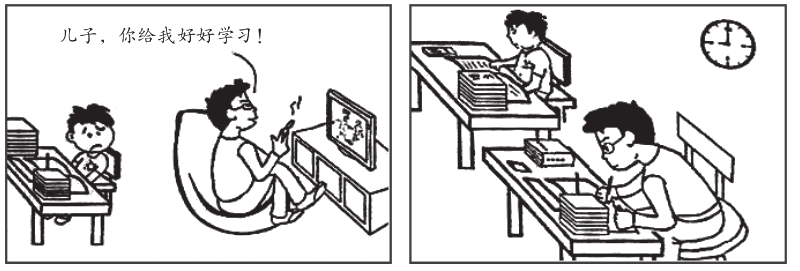
\includegraphics[width=0.87\linewidth]{picture/2016.png}
	\caption*{与其只提要求,不如做个榜样}
\end{figure}


\checkpagenumber%

\bta{2017}


\section{Use of English}

\noindent
\textbf{Directions:}
Read the following text. Choose the best word (s) for each numbered blank
and mark A, B, C or D on the ANSWER SHEET. (10 points)


\TiGanSpace


Could a hug a day keep the doctor away? The answer may be a resounding
``yes!'' \cloze helping you feel close and \cloze to
people you care about, it turns out that hugs can bring a \cloze
of health benefits to your body and mind. Believe it or not, a warm
embrace might even help you \cloze getting sick this winter.

In a recent study \cloze over 400 healthy adults, researchers
from Carnegie Mellon University in Pennsylvania examined the effects of
perceived social support and the receipt of hugs \cloze the
participants' susceptibility to developing the common cold after being
\cloze to the virus. People who perceived greater social support
were less likely to come \cloze with a cold, and the researchers
\cloze that the stress-reducing effects of hugging \cloze
about 32 percent of that beneficial effect. \cloze among those
who got a cold, the ones who felt greater social support and received
more frequent hugs had less severe \cloze.

``Hugging protects people who are under stress from the \cloze
risk for colds that's usually \cloze with stress,'' notes
Sheldon Cohen, a professor of psychology at Carnegie. Hugging ``is a
marker of intimacy and helps \cloze the feeling that others are
there to help \cloze difficulty.''

Some experts \cloze the stress-reducing, health-related
benefits of hugging to the release of oxytocin, often called ``the
bonding hormone'' \cloze it promotes attachment in
relationships, including that between mothers and their newborn babies.
Oxytocin is made primarily in the central lower part of the brain, and
some of it is released into the bloodstream. But some of it
\cloze in the brain, where it \cloze mood, behavior and
physiology.


\newpage

\begin{enumerate}
	%\renewcommand{\labelenumi}{\arabic{enumi}.}
	% A(\Alph) a(\alph) I(\Roman) i(\roman) 1(\arabic)
	%设定全局标号series=example	%引用全局变量resume=example
	%[topsep=-0.3em,parsep=-0.3em,itemsep=-0.3em,partopsep=-0.3em]
	%可使用leftmargin调整列表环境左边的空白长度 [leftmargin=0em]
	\item


\fourchoices
{Unlike}
{Besides}
{Throughout}
{Despite}




\item


\fourchoices
{equal}
{restricted}
{connected}
{inferior}




\item


\fourchoices
{host}
{view}
{lesson}
{choice}




\item


\fourchoices
{recall}
{forget}
{avoid}
{keep}




\item

\fourchoices
{collecting}
{affecting}
{guiding}
{involving}


\item


\fourchoices
{on}
{in}
{at}
{of}




\item


\fourchoices
{devoted}
{exposed}
{lost}
{attracted}




\item


\fourchoices
{along}
{across}
{down}
{out}




\item


\fourchoices
{imagined}
{denied}
{doubted}
{calculated}




\item


\fourchoices
{served}
{explained}
{restored}
{required}




\item


\fourchoices
{Thus}
{Still}
{Rather}
{Even}




\item


\fourchoices
{defeats}
{symptoms}
{errors}
{tests}




\item

\fourchoices
{highlighted}
{minimized}
{controlled}
{increased}



\item

\fourchoices
{associated}
{equipped}
{presented}
{compared}


\item


\fourchoices
{assess}
{moderate}
{generate}
{record}




\item

\fourchoices
{in the face of}
{in the form of}
{in the name of}
{in the way of}


\item


\fourchoices
{attribute}
{commit}
{transfer}
{return}




\item


\fourchoices
{unless}
{because}
{though}
{until}




\item


\fourchoices
{vanishes}
{emerges}
{remains}
{decreases}




\item

\fourchoices
{experiences}
{combines}
{justifies}
{influences}



\end{enumerate}


\hfill

\section{Reading Comprehension}


\noindent
\textbf{Part A}\\
\textbf{Directions:}\\
Read the following four texts. Answer the questions below each text by
choosing A, B, C or
D. Mark your answers on the ANSWER SHEET. (40 points)

\newpage
\subsection{Text 1}


First two hours, now three hours---this is how far in advance
authorities are recommending people show up to catch a domestic flight,
at least at some major U.S. airports with increasingly massive security
lines.

Americans are willing to tolerate time-consuming security procedures in
return for increased safety. The crash of EgyptAir Flight 804, which
terrorists may have downed over the Mediterranean Sea, provides another
tragic reminder of why. But demanding too much of air travelers or
providing too little security in return undermines public support for
the process. And it should: Wasted time is a drag on Americans'
economic and private lives, not to mention infuriating.

Last year, the Transportation Security Administration (TSA) found in a
secret check that undercover investigators were able to sneak
weapons---both fake and real---past airport security nearly every time
they tried. Enhanced security measures since then, combined with a rise
in airline travel due to the improving economy and low oil prices, have
resulted in long waits at major airports such as Chicago's O'Hare
International. It is not yet clear how much more effective airline
security has become---but the lines are obvious.

Part of the issue is that the government did not anticipate the steep
increase in airline travel, so the TSA is now rushing to get new
screeners on the line. Part of the issue is that airports have only so
much room for screening lanes. Another factor may be that more people
are trying to overpack their carry-on bags to avoid checked-baggage
fees, though the airlines strongly dispute this.

There is one step the TSA could take that would not require remodeling
airports or rushing to hire: Enroll more people in the PreCheck program.
PreCheck is supposed to be a win-win for travelers and the TS
A.
Passengers who pass a background check are eligible to use
\uline{expedited} screening lanes. This allows the TSA to focus on
travelers who are higher risk, saving time for everyone involved. The
TSA wants to enroll 25 million people in PreCheck.

It has not gotten anywhere close to that, and one big reason is sticker
shock: Passengers must pay \$85 every five years to process their
background checks. Since the beginning, this price tag has been
PreCheck's fatal flaw. Upcoming reforms might bring the price to a more
reasonable level. But Congress should look into doing so directly, by
helping to finance PreCheck enrollment or to cut costs in other ways.

The TSA cannot continue diverting resources into underused PreCheck
lanes while most of the traveling public suffers in unnecessary lines.
It is long past time to make the program work.

\begin{enumerate}[resume]
	%\renewcommand{\labelenumi}{\arabic{enumi}.}
	% A(\Alph) a(\alph) I(\Roman) i(\roman) 1(\arabic)
	%设定全局标号series=example	%引用全局变量resume=example
	%[topsep=-0.3em,parsep=-0.3em,itemsep=-0.3em,partopsep=-0.3em]
	%可使用leftmargin调整列表环境左边的空白长度 [leftmargin=0em]
	\item
The crash of EgyptAir Flight 804 is mentioned to \lineread.


\fourchoices
{explain Americans' tolerance of current security checks}
{stress the urgency to strengthen security worldwide}
{highlight the necessity of upgrading major U.S. airports}
{emphasize the importance of privacy protection}



\item
Which of the following contributes to long waits at major airports?


\fourchoices
{New restrictions on carry-on bags.}
{The declining efficiency of the TSA.}
{An increase in the number of travelers.}
{Frequent unexpected secret checks.}



\item
The word ``expedited'' (Line 4, Para. 5) is closest in meaning to \lineread.


\fourchoices
{quieter}
{cheaper}
{wider}
{faster}





\item
One problem with the PreCheck program is  \lineread.


\fourchoices
{a dramatic reduction of its scale}
{its wrongly-directed implementation}
{the government's reluctance to back it}
{an unreasonable price for enrollment}


\item
Which of the following would be the best title for the text?


\fourchoices
{Less Screening for More Safety}
{PreCheck---a Belated Solution}
{Getting Stuck in Security Lines}
{Underused PreCheck Lanes}


\end{enumerate}


\newpage
\subsection{Text 2}


``The ancient Hawaiians were astronomers,'' wrote Queen Liliuokalani,
Hawaii's last reigning monarch, in 1897. Star watchers were among the
most esteemed members of Hawaiian society. Sadly, all is not well with
astronomy in Hawaii today. Protests have erupted over construction of
the Thirty Meter Telescope (TMT), a giant observatory that promises to
revolutionize humanity's view of the cosmos.

At issue is the TMT's planned location on Mauna Kea, a dormant volcano
worshiped by some Hawaiians as the \emph{piko}, that connects the
Hawaiian Islands to the heavens. But Mauna Kea is also home to some of
the world's most powerful telescopes. Rested in the Pacific Ocean,
Mauna Kea's peak rises above the bulk of our planet's dense atmosphere,
where conditions allow telescopes to obtain images of unsurpassed
clarity.

Opposition to telescopes on Mauna Kea is nothing new. A small but
vocal group of Hawaiians and environmentalists have long viewed their
presence as disrespect for sacred land and a painful reminder of the
occupation of what was once a sovereign nation.

Some blame for the current controversy belongs to astronomers. In
their eagerness to build bigger telescopes, they forgot that science is
not the only way of understanding the world. They did not always
prioritize the protection of Mauna Kea's fragile ecosystems or its
holiness to the islands' inhabitants. Hawaiian culture is not a relic
of the past; it is a living culture undergoing a renaissance today.

Yet science has a cultural history, too, with roots going back to the
dawn of civilization. The same curiosity to find what lies beyond the
horizon that first brought early Polynesians to Hawaii's shores inspires
astronomers today to explore the heavens. Calls to disassemble all
telescopes on Mauna Kea or to ban future development there ignore the
reality that astronomy and Hawaiian culture both seek to answer big
questions about who we are, where we come from and where we are going.
Perhaps that is why we explore the starry skies, as if answering a
primal calling to know ourselves and our true ancestral homes.

The astronomy community is making compromises to change its use of
Mauna Kea. The TMT site was chosen to minimize the telescope's
visibility around the island and to avoid archaeological and
environmental impact. To limit the number of telescopes on Mauna Kea,
old ones will be removed at the end of their lifetimes and their sites
returned to a natural state. There is no reason why everyone cannot be
welcomed on Mauna Kea to embrace their cultural heritage and to study
the stars.

\begin{enumerate}[resume]
	%\renewcommand{\labelenumi}{\arabic{enumi}.}
	% A(\Alph) a(\alph) I(\Roman) i(\roman) 1(\arabic)
	%设定全局标号series=example	%引用全局变量resume=example
	%[topsep=-0.3em,parsep=-0.3em,itemsep=-0.3em,partopsep=-0.3em]
	%可使用leftmargin调整列表环境左边的空白长度 [leftmargin=0em]
	\item
Queen Liliuokalani's remark in Paragraph 1 indicates \lineread.


\fourchoices
{her conservative view on the historical role of astronomy}
{the importance of astronomy in ancient Hawaiian society}
{the regrettable decline of astronomy in ancient times}
{her appreciation of star watchers' feats in her time}




\item
Mauna Kea is deemed as an ideal astronomical site due to \lineread.


\fourchoices
{its geographical features}
{its protective surroundings}
{its religious implications}
{its existing infrastructure}


\item
The construction of the TMT is opposed by some locals partly because \lineread.


\fourchoices
{it may risk ruining their intellectual life}
{it reminds them of a humiliating history}
{their culture will lose a chance of revival}
{they fear losing control of Mauna Kea}




\item
It can be inferred from Paragraph 5 that progress in today's
astronomy \lineread.

\fourchoices
{is fulfilling the dreams of ancient Hawaiians}
{helps spread Hawaiian culture across the world}
{may uncover the origin of Hawaiian culture}
{will eventually soften Hawaiians' hostility}


\item
The author's attitude toward choosing Mauna Kea as the TMT site is
one of \lineread.


\fourchoices
{severe criticism}
{passive acceptance}
{slight hesitancy}
{full approval}



\end{enumerate}


\newpage
\subsection{Text 3}


Robert F. Kennedy once said that a country's GDP measures ``everything
except that which makes life worthwhile.'' With Britain voting to leave
the European Union, and GDP already predicted to slow as a result, it is
now a timely moment to assess what he was referring to.

The question of GDP and its usefulness has annoyed policymakers for
over half a century. Many argue that it is a flawed concept. It
measures things that do not matter and misses things that do. By most
recent measures, the UK's GDP has been the envy of the Western world,
with record low unemployment and high growth figures. If everything was
going so well, then why did over 17 million people vote for Brexit,
despite the warnings about what it could do to their country's economic
prospects?

A recent annual study of countries and their ability to convert growth
into well-being sheds some light on that question. Across the 163
countries measured, the UK is one of the poorest performers in ensuring
that economic growth is translated into meaningful improvements for its
citizens. Rather than just focusing on GDP, over 40 different sets of
criteria from health, education and civil society engagement have been
measured to get a more rounded assessment of how countries are
performing.

While all of these countries face their own challenges, there are a
number of consistent themes. Yes, there has been a budding economic
recovery since the 2008 global crash, but in key indicators in areas
such as health and education, major economies have continued to decline.
Yet this isn't the case with all countries. Some relatively poor
European countries have seen huge improvements across measures including
civil society, income equality and the environment.

This is a lesson that rich countries can learn: When GDP is no longer
regarded as the sole measure of a country's success, the world looks
very different.

So, what Kennedy was referring to was that while GDP has been the most
common method for measuring the economic activity of nations, as a
measure, it is no longer enough. It does not include important factors
such as environmental quality or education outcomes---all things that
contribute to a person's sense of well-being.

The sharp hit to growth predicted around the world and in the UK could
lead to a decline in the everyday services we depend on for our
well-being and for growth. But policymakers who refocus efforts on
improving well-being rather than simply worrying about GDP figures could
avoid the forecasted doom and may even see progress.


\begin{enumerate}[resume]
	%\renewcommand{\labelenumi}{\arabic{enumi}.}
	% A(\Alph) a(\alph) I(\Roman) i(\roman) 1(\arabic)
	%设定全局标号series=example	%引用全局变量resume=example
	%[topsep=-0.3em,parsep=-0.3em,itemsep=-0.3em,partopsep=-0.3em]
	%可使用leftmargin调整列表环境左边的空白长度 [leftmargin=0em]
	\item
Robert F. Kennedy is cited because he  \lineread.


\fourchoices
{praised the UK for its GDP}
{identified GDP with happiness}
{misinterpreted the role of GDP}
{had a low opinion of GDP}



\item
It can be inferred from Paragraph 2 that  \lineread.


\fourchoices
{the UK is reluctant to remold its economic pattern}
{the UK will contribute less to the world economy}
{GDP as the measure of success is widely defied in the UK}
{policymakers in the UK are paying less attention to GDP}


\item
Which of the following is true about the recent annual study?


\fourchoices
{It excludes GDP as an indicator.}
{It is sponsored by 163 countries.}
{Its criteria are questionable.}
{Its results are enlightening.}


\item
 In the last two paragraphs, the author suggests that \lineread.


\fourchoices
{the UK is preparing for an economic boom}
{high GDP foreshadows an economic decline}
{it is essential to consider factors beyond GDP}
{it requires caution to handle economic issues}



\item
Which of the following is the best title for the text?


\fourchoices
{High GDP But Inadequate Well-being, a UK Lesson}
{GDP Figures, a Window on Global Economic Health}
{Robert F. Kennedy, a Terminator of GDP}
{Brexit, the UK's Gateway to Well-being}
	
\end{enumerate}


\newpage
\subsection{Text 4}


In a rare unanimous ruling, the US Supreme Court has overturned the
corruption conviction of a former Virginia governor, Robert McDonnell.
\uline{But it did so while holding its nose at the ethics of his
	conduct}, which included accepting gifts such as a Rolex watch and a
Ferrari automobile from a company seeking access to government.

The high court's decision said the judge in Mr. McDonnell's trial
failed to tell a jury that it must look only at his ``official acts,''
or the former governor's decisions on ``specific'' and ``unsettled''
issues related to his duties.

Merely helping a gift-giver gain access to other officials, unless done
with clear intent to pressure those officials, is not corruption, the
justices found.

The court did suggest that accepting favors in return for opening doors
is ``distasteful'' and ``nasty.'' But under anti-bribery laws, proof
must be made of concrete benefits, such as approval of a contract or
regulation. Simply arranging a meeting, making a phone call, or hosting
an event is not an ``official act.''

The court's ruling is legally sound in defining a kind of favoritism
that is not criminal. Elected leaders must be allowed to help
supporters deal with bureaucratic problems without fear of prosecution
of bribery. ``The basic compact underlying representative government,''
wrote Chief Justice John Roberts for the court, ``assumes that public
officials will hear from their constituents and act on their concerns.''

But the ruling reinforces the need for citizens and their elected
representatives, not the courts, to ensure equality of access to
government. Officials must not be allowed to play favorites in
providing information or in arranging meetings simply because an
individual or group provides a campaign donation or a personal gift.
This type of integrity requires well-enforced laws in government
transparency, such as records of official meetings, rules on lobbying,
and information about each elected leader's source of wealth.

Favoritism in official access can fan public perceptions of corruption.
But it is not always corruption. Rather officials must avoid double
standards, or different types of access for average people and the
wealthy. If connections can be bought, a basic premise of democratic
society---that all are equal in treatment by government---is
undermined. Good governance rests on an understanding of the inherent
worth of each individual.

The court's ruling is a step forward in the struggle against both
corruption and official favoritism.

\begin{enumerate}[resume]
	%\renewcommand{\labelenumi}{\arabic{enumi}.}
	% A(\Alph) a(\alph) I(\Roman) i(\roman) 1(\arabic)
	%设定全局标号series=example	%引用全局变量resume=example
	%[topsep=-0.3em,parsep=-0.3em,itemsep=-0.3em,partopsep=-0.3em]
	%可使用leftmargin调整列表环境左边的空白长度 [leftmargin=0em]
	\item
The underlined sentence (Para. 1) most probably shows that the court \lineread.

\fourchoices
{avoided defining the extent of McDonnell's duties}
{made no compromise in convicting McDonnell}
{was contemptuous of McDonnell's conduct}
{refused to comment on McDonnell's ethics}



\item
 According to Paragraph 4, an official act is deemed corruptive only
if it involves \lineread.


\fourchoices
{concrete returns for gift-givers}
{sizable gains in the form of gifts}
{leaking secrets intentionally}
{breaking contracts officially}



\item
The court's ruling is based on the assumption that public officials
are \lineread.


\fourchoices
{allowed to focus on the concerns of their supporters}
{qualified to deal independently with bureaucratic issues}
{justified in addressing the needs of their constituents}
{exempt from conviction on the charge of favoritism}


\item
Well-enforced laws in government transparency are needed to \lineread.


\fourchoices
{awaken the conscience of officials}
{guarantee fair play in official access}
{allow for certain kinds of lobbying}
{inspire hopes in average people}



\item
The author's attitude toward the court's ruling is \lineread.


\fourchoices
{sarcastic}
{tolerant}
{skeptical}
{supportive}





\end{enumerate}

\newpage

\noindent
\textbf{Part B}\\
\textbf{Directions:}\\
The following paragraphs are given in a wrong order. For questions
41-45, you are required to reorganize these paragraphs into a coherent
text by choosing from the list A-G and filling them into the numbered
boxes. Paragraphs B and D have been correctly placed. Mark your
answers on the ANSWER SHEET. (10 points)


\begin{listmatch}


\item 
The first published sketch, ``A Dinner at Poplar Walk'' brought tears
to Dickens's eyes when he discovered it in the pages of \emph{The Monthly Magazine}. From then on his sketches, which appeared under the
pen name ``Boz'' in \emph{The Evening Chronicle}, earned him a modest
reputation.


\item 
The runaway success of \emph{The Pickwick Papers}, as it is generally
known today, secured Dickens's fame. There were Pickwick coats and
Pickwick cigars, and the plump, spectacled hero, Samuel Pickwick, became
a national figure.


\item 
Soon after \emph{Sketches by Boz} appeared, a publishing firm
approached Dickens to write a story in monthly installments, as a
backdrop for a series of woodcuts by the then-famous artist Robert
Seymour, who had originated the idea for the story. With characteristic
confidence, Dickens successfully insisted that Seymour's pictures
illustrate his own story instead. After the first installment, Dickens
wrote to the artist and asked him to correct a drawing Dickens felt was
not faithful enough to his prose. Seymour made the change, went into his
backyard, and expressed his displeasure by committing suicide. Dickens
and his publishers simply pressed on with a new artist. The comic novel,
\emph{The Posthumous Papers of the Pickwick Club}, appeared serially in
1836 and 1837 and was first published in book form in 1837.


\item 
Charles Dickens is probably the best-known and, to many people, the
greatest English novelist of the 19th century. A moralist, satirist, and
social reformer, Dickens crafted complex plots and striking characters
that capture the panorama of English society.


\item 
Soon after his father's release from prison, Dickens got a better job
as errand boy in law offices. He taught himself shorthand to get an even
better job later as a court stenographer and as a reporter in
Parliament. At the same time, Dickens, who had a reporter's eye for
transcribing the life around him, especially anything comic or odd,
submitted short sketches to obscure magazines.


\item 
Dickens was born in Portsmouth, on England's southern coast. His
father was a clerk in the British Navy pay office---a respectable
position, but with little social status. His paternal grandparents, a
steward and a housekeeper, possessed even less status, having been
servants, and Dickens later concealed their background. Dicken's mother
supposedly came from a more respectable family. Yet two years before
Dicken's birth, his mother's father was caught stealing and fled to
Europe, never to return. The family's increasing poverty forced Dickens
out of school at age 12 to work in Warren's Blacking Warehouse, a
shoe-polish factory, where the other working boys mocked him as ``the
young gentleman.'' His father was then imprisoned for debt. The
humiliations of his father's imprisonment and his labor in the blacking
factory formed Dickens's greatest wound and became his deepest secret.
He could not confide them even to his wife, although they provide the
unacknowledged foundation of his fiction.


\item 
After \emph{Pickwick}, Dickens plunged into a bleaker world. In
\emph{Oliver Twist}, he traces an orphan's progress from the workhouse
to the criminal slums of London. \emph{Nicholas Nickleby}, his next
novel, combines the darkness of \emph{Oliver Twist} with the sunlight of
\emph{Pickwick}. The popularity of these novels consolidated Dickens' as
a nationally and internationally celebrated man of letters.



\end{listmatch}


\[ 
\begin{tabular}{|c|}
	\hline
	D \\
	\hline
\end{tabular}
\rightarrow
\begin{tabular}{|c|c|}
	\hline
	41. &  \hspace{1.5em} \\
	\hline
\end{tabular}
\rightarrow
\begin{tabular}{|c|c|}
	\hline
	42. &  \hspace{1.5em} \\
	\hline
\end{tabular}
\rightarrow
\begin{tabular}{|c|c|}
	\hline
	43. &  \hspace{1.5em} \\
	\hline
\end{tabular}
\rightarrow
\begin{tabular}{|c|c|}
	\hline
	44. &  \hspace{1.5em} \\
	\hline
\end{tabular}
\rightarrow
\begin{tabular}{|c|}
	\hline
	E \\
	\hline
\end{tabular}
\rightarrow
\begin{tabular}{|c|c|}
	\hline
	45. &  \hspace{1.5em} \\
	\hline
\end{tabular}
\]


\phantom{ \linefill \linefill \linefill \linefill \linefill}



\newpage
\noindent
\textbf{Part C}\\
\textbf{Directions:}\\
Read the following text carefully and then translate the underlined
segments into Chinese. Your translation should be written neatly on the
ANSWER SHEET. (10 points)


\TiGanSpace

The growth of the use of English as the world's primary language for
international communication has obviously been continuing for several
decades. \transnum \uline{But even as the number of English speakers
	expands further there are signs that the global predominance of the
	language may fade within the foreseeable future}.

Complex international, economic, technological and cultural changes
could start to diminish the leading position of English as the language
of the world market, and UK interests which enjoy advantage from the
breadth of English usage would consequently face new pressures. Those
realistic possibilities are highlighted in the study presented by David
Graddol. \transnum \uline{His analysis should therefore end any
	self-contentedness among those who may believe that the global position
	of English is so stable that the young generations of the United Kingdom
	do not need additional language capabilities}.

David Graddol concludes that monoglot English graduates face a bleak
economic future as qualified multilingual youngsters from other
countries are proving to have a competitive advantage over their British
counterparts in global companies and organisations. Alongside that,
\transnum \uline{many countries are introducing English into the
	primary-school curriculum but British schoolchildren and students do not
	appear to be gaining greater encouragement to achieve fluency in other
	languages}.

If left to themselves, such trends will diminish the relative strength
of the English language in international education markets as the demand
for educational resources in languages, such as Spanish, Arabic or
Mandarin grows and international business process outsourcing in other
languages such as Japanese, French and German, spreads.

\transnum \uline{The changes identified by David Graddol all present
	clear and major challenges to the UK's providers of English language
	teaching to people of other countries and to broader education business
	sectors.} The English language teaching sector directly earns nearly
£1.3 billion for the UK in invisible exports and our other education
related exports earn up to £10 billion a year more. As the international
education market expands, the recent slowdown in the numbers of
international students studying in the main English-speaking countries
is likely to continue, especially if there are no effective strategic
policies to prevent such slippage.

The anticipation of possible shifts in demand provided by this study is
significant: \transnum \uline{It gives a basis for all organisations
	which seek to promote the learning and use of English, a basis for
	planning to meet the possibilities of what could be a very different
	operating environment}. That is a necessary and practical approach. In
this as in much else, those who wish to influence the future must
prepare for it.


\newpage

\section{Writing}


\noindent
\textbf{Part A}\\
\textbf{51. Directions:}

You are to write an email to James Cook, a newly-arrived Australian
professor, recommending some tourist attractions in your city. Please
give reasons for your recommendation.

You should write neatly on the ANSWER SHEET.

\textbf{Do not} sign your own name at the end of the email. Use ``Li
Ming'' instead.

\textbf{Do not} write the address. (10 points)

\vspace{2em}

\noindent
\textbf{Part B}\\
\textbf{52. Directions:}

Write an essay of 160---200 words based on the following pictures. In
your essay, you should
\begin{listwrite}
	%\renewcommand{\labelenumi}{\arabic{enumi}.}
	% A(\Alph) a(\alph) I(\Roman) i(\roman) 1(\arabic)
	%设定全局标号series=example	%引用全局变量resume=example
	%[topsep=-0.3em,parsep=-0.3em,itemsep=-0.3em,partopsep=-0.3em]
	%可使用leftmargin调整列表环境左边的空白长度 [leftmargin=0em]
	\item
describe the pictures briefly,

\item 
 interpret the meaning, and

\item 
 give your comments.
\end{listwrite}

You should write neatly on the ANSWER SHEET. (20 points)


\begin{figure}[h!]
	\centering
	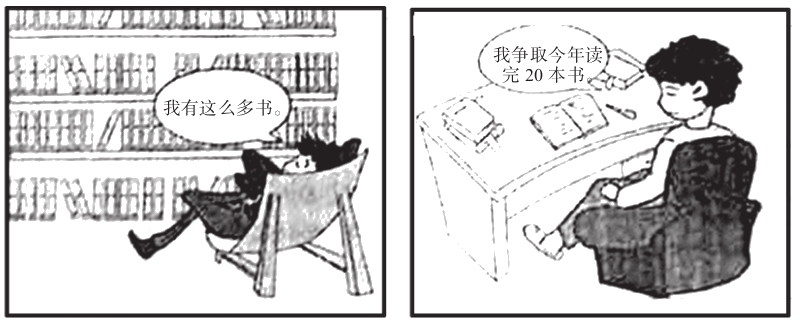
\includegraphics[width=0.87\linewidth]{picture/2017.png}
	\caption*{“有书”与“读书”}
\end{figure}



%


\bta{2018}



\section{Use of English}

\noindent
\textbf{Directions:}\\
Read the following text. Choose the best word (s) for each numbered blank
and mark A, B, C or D on the ANSWER SHEET. (10 points)



\TiGanSpace

Trust is a tricky business. On the one hand, it's a necessary
condition \cloze many worthwhile things: child care, friendships,
etc. On the other hand, putting your \cloze in the wrong place
often carries a high \cloze.

\cloze , why do we trust at all? Well, because it feels good.
\cloze people place their trust in an individual or an
institution, their brains release oxytocin, a hormone that \cloze
pleasurable feelings and triggers the herding instinct that prompts
humans to \cloze with one another. Scientists have found that
exposure \cloze this hormone puts us in a trusting \cloze
: In a Swiss study, researchers sprayed oxytocin into the noses of half
the subjects; those subjects were ready to lend significantly higher
amounts of money to strangers than were their \cloze who inhaled
something else.

\cloze for us, we also have a sixth sense for dishonesty that
may \cloze us. A Canadian study found that children as young as
14 months can differentiate \cloze a credible person and a
dishonest one. Sixty toddlers were each \cloze to an adult
tester holding a plastic container. The tester would ask, " What's in
here?" before looking into the container, smiling, and exclaiming,
" Wow!" Each subject was then invited to look \cloze. Half of
them found a toy; the other half \cloze the container was
empty---and realized the tester had \cloze them.

Among the children who had not been tricked, the majority were
\cloze to cooperate with the tester in learning a new skill,
demonstrating that they trusted his leadership. \cloze , only
five of the 30 children paired with the " \cloze " tester
participated in a follow-up activity.



\newpage

\begin{enumerate}
	%\renewcommand{\labelenumi}{\arabic{enumi}.}
	% A(\Alph) a(\alph) I(\Roman) i(\roman) 1(\arabic)
	%设定全局标号series=example	%引用全局变量resume=example
	%[topsep=-0.3em,parsep=-0.3em,itemsep=-0.3em,partopsep=-0.3em]
	%可使用leftmargin调整列表环境左边的空白长度 [leftmargin=0em]
	\item

\fourchoices
{from}
{for}
{like}
{on}



\item

\fourchoices
{attention}
{concern}
{faith}
{interest}



\item

\fourchoices
{benefit}
{price}
{debt}
{hope}


\item

\fourchoices
{Again}
{Instead}
{Therefore}
{Then}



\item

\fourchoices
{When}
{Unless}
{Although}
{Until}


\item

\fourchoices
{selects}
{applies}
{produces}
{maintains}



\item

\fourchoices
{connect}
{compete}
{consult}
{compare}



\item

\fourchoices
{by}
{to}
{of}
{at}


\item

\fourchoices
{context}
{circle}
{period}
{mood}



\item

\fourchoices
{counterparts}
{colleagues}
{substitutes}
{supporters}



\item

\fourchoices
{Odd}
{Funny}
{Lucky}
{Ironic}


\item

\fourchoices
{protect}
{delight}
{surprise}
{monitor}


\item

\fourchoices
{over}
{within}
{toward}
{between}


\item

\fourchoices
{added}
{transferred}
{introduced}
{entrusted}



\item

\fourchoices
{out}
{inside}
{back}
{around}


\item

\fourchoices
{proved}
{remembered}
{insisted}
{discovered}


\item

\fourchoices
{fooled}
{mocked}
{betrayed}
{wronged}



\item

\fourchoices
{forced}
{willing}
{hesitant}
{entitled}


\item

\fourchoices
{On the whole}
{As a result}
{For instance}
{In contrast}


\item

\fourchoices
{incapable}
{inflexible}
{unreliable}
{unsuitable}

\end{enumerate}

\vfil

\section{Reading Comprehension}


\noindent
\textbf{Part A}\\
\textbf{Directions:}\\
Read the following four texts. Answer the questions after each text by
choosing A, B, C or
D. Mark your answers on the ANSWER SHEET. (40
points)

\newpage
\subsection{Text 1}


Among the annoying challenges facing the middle class is one that will
probably go unmentioned in the next presidential campaign: What happens
when the robots come for their jobs?

Don't dismiss that possibility entirely. About half of U.S. jobs are
at high risk of being automated, according to a University of Oxford
study, with the middle class disproportionately squeezed. Lower-income
jobs like gardening or day care don't appeal to robots. But many
middle-class occupations---trucking, financial advice, software
engineering---have aroused their interest, or soon will. The rich own
the robots, so they will be fine.

This isn't to be alarmist. Optimists point out that technological
upheaval has benefited workers in the past. The Industrial Revolution
didn't go so well for Luddites whose jobs were displaced by mechanized
looms, but it eventually raised living standards and created more jobs
than it destroyed. Likewise, automation should eventually boost
productivity, stimulate demand by driving down prices, and free workers
from hard, boring work. But in the medium term, middle-class workers
may need a lot of help adjusting.

The first step, as Erik Brynjolfsson and Andrew McAfee argue in
\emph{The Second Machine Age}, should be rethinking education and job
training. Curriculums---from grammar school to college---should evolve
to focus less on memorizing facts and more on creativity and complex
communication. Vocational schools should do a better job of fostering
problem-solving skills and helping students work alongside robots.
Online education can supplement the traditional kind. It could make
extra training and instruction affordable. Professionals trying to
acquire new skills will be able to do so without going into debt.

The challenge of coping with automation underlines the need for the
U.S. to revive its fading business dynamism: Starting new companies must
be made easier. In previous eras of drastic technological change,
entrepreneurs smoothed the transition by dreaming up ways to combine
labor and machines. The best uses of 3 D printers and virtual reality
haven't been invented yet. The U.S. needs the new companies that will
invent them.

Finally, because automation threatens to widen the gap between capital
income and labor income, taxes and the safety net will have to be
rethought. Taxes on low-wage labor need to be cut, and wage subsidies
such as the earned income tax credit should be expanded: This would
boost incomes, encourage work, reward companies for job creation, and
reduce inequality.

Technology will improve society in ways big and small over the next few
years, yet this will be little comfort to those who find their lives and
careers upended by automation. Destroying the machines that are coming
for our jobs would be nuts. But policies to help workers adapt will be
indispensable.

\begin{enumerate}[resume]
	%\renewcommand{\labelenumi}{\arabic{enumi}.}
	% A(\Alph) a(\alph) I(\Roman) i(\roman) 1(\arabic)
	%设定全局标号series=example	%引用全局变量resume=example
	%[topsep=-0.3em,parsep=-0.3em,itemsep=-0.3em,partopsep=-0.3em]
	%可使用leftmargin调整列表环境左边的空白长度 [leftmargin=0em]
	\item
Who will be most threatened by automation?


\fourchoices
{Leading politicians.}
{Low-wage laborers.}
{Robot owners.}
{Middle-class workers.}


\item
Which of the following best represents the author's view?


\fourchoices
{Worries about automation are in fact groundless.}
{Optimists' opinions on new tech find little support.}
{Issues arising from automation need to be tackled.}
{Negative consequences of new tech can be avoided.}


\item
Education in the age of automation should put more emphasis on \lineread.


\fourchoices
{creative potential}
{job-hunting skills}
{individual needs}
{cooperative spirit}


\item
The author suggests that tax policies be aimed at \lineread.


\fourchoices
{encouraging the development of automation}
{increasing the return on capital investment}
{easing the hostility between rich and poor}
{preventing the income gap from widening}

\item
In this text, the author presents a problem with \lineread.


\fourchoices
{opposing views on it}
{possible solutions to it}
{its alarming impacts}
{its major variations}

\end{enumerate}


\newpage
\subsection{Text 2}


A new survey by Harvard University finds more than two-thirds of young
Americans disapprove of President Trump's use of Twitter. The
implication is that Millennials prefer news from the White House to be
filtered through other sources, not a president's social media platform.

Most Americans rely on social media to check daily headlines. Yet as
distrust has risen toward all media, people may be starting to
\uline{beef up} their media literacy skills. Such a trend is badly
needed. During the 2016 presidential campaign, nearly a quarter of web
content shared by Twitter users in the politically critical state of
Michigan was fake news, according to the University of Oxford. And a
survey conducted for BuzzFeed News found 44 percent of Facebook users
rarely or never trust news from the media giant.

Young people who are digital natives are indeed becoming more skillful
at separating fact from fiction in cyberspace. A Knight Foundation
focus-group survey of young people between ages 14 and 24 found they use
``distributed trust'' to verify stories. They cross-check sources and
prefer news from different perspectives---especially those that are open
about any bias. ``Many young people assume a great deal of personal
responsibility for educating themselves and actively seeking out
opposing viewpoints,'' the survey concluded.

Such active research can have another effect. A 2014 survey conducted
in Australia, Britain, and the United States by the University of
Wisconsin-Madison found that young people's reliance on social media led
to greater political engagement.

Social media allows users to experience news events more intimately and
immediately while also permitting them to re-share news as a projection
of their values and interests. This forces users to be more conscious
of their role in passing along information. A survey by Barna research
group found the top reason given by Americans for the fake news
phenomenon is ``reader error,'' more so than made-up stories or factual
mistakes in reporting. About a third say the problem of fake news lies
in ``misinterpretation or exaggeration of actual news'' via social
media. In other words, the choice to share news on social media may be
the heart of the issue. ``This indicates there is a real personal
responsibility in counteracting this problem,'' says Roxanne Stone,
editor in chief at Barna Group.

So when young people are critical of an over-tweeting president, they
reveal a mental discipline in thinking skills---and in their choices on
when to share on social media.


\begin{enumerate}[resume]
	%\renewcommand{\labelenumi}{\arabic{enumi}.}
	% A(\Alph) a(\alph) I(\Roman) i(\roman) 1(\arabic)
	%设定全局标号series=example	%引用全局变量resume=example
	%[topsep=-0.3em,parsep=-0.3em,itemsep=-0.3em,partopsep=-0.3em]
	%可使用leftmargin调整列表环境左边的空白长度 [leftmargin=0em]
	\item
According to Paragraphs 1 and 2, many young Americans cast doubt on \lineread.


\fourchoices
{the justification of the news-filtering practice}
{people's preference for social media platforms}
{the administration's ability to handle information}
{social media as a reliable source of news}


\item
The phrase " beef up'' (Para. 2) is closest in meaning to \lineread.


\fourchoices
{sharpen}
{define}
{boast}
{share}



\item
According to the Knight Foundation survey, young people \lineread.


\fourchoices
{tend to voice their opinions in cyberspace}
{verify news by referring to diverse sources}
{have a strong sense of social responsibility}
{like to exchange views on ``distributed trust''}


\item
The Barna survey found that a main cause for the fake news problem
is \lineread.


\fourchoices
{readers' outdated values}
{journalists' biased reporting}
{readers' misinterpretation}
{journalists' made-up stories}


\item
Which of the following would be the best title for the text?


\fourchoices
{A Rise in Critical Skills for Sharing News Online}
{A Counteraction Against the Over-tweeting Trend}
{The Accumulation of Mutual Trust on Social Media}
{The Platforms for Projection of Personal Interests}


\end{enumerate}


\newpage
\subsection{Text 3}


Any fair-minded assessment of the dangers of the deal between Britain's
National Health Service (NHS) and DeepMind must start by acknowledging
that both sides mean well. DeepMind is one of the leading artificial
intelligence (AI) companies in the world. The potential of this work
applied to healthcare is very great, but it could also lead to further
concentration of power in the tech giants. It is against that
background that the information commissioner, Elizabeth Denham, has
issued her damning verdict against the Royal Free Hospital trust under
the NHS, which handed over to DeepMind the records of 1.6 million
patients in 2015 on the basis of a vague agreement which took far too
little account of the patients' rights and their expectations of
privacy.

DeepMind has almost apologized. The NHS trust has mended its ways.
Further arrangements---and there may be many---between the NHS and
DeepMind will be carefully scrutinised to ensure that all necessary
permissions have been asked of patients and all unnecessary data has
been cleaned. There are lessons about informed patient consent to
learn. But privacy is not the only angle in this case and not even the
most important. Ms Denham chose to concentrate the blame on the NHS
trust, since under existing law it ``controlled'' the data and DeepMind
merely ``processed'' it. But this distinction misses the point that it
is processing and aggregation, not the mere possession of bits, that
gives the data value.

The great question is who should benefit from the analysis of all the
data that our lives now generate. Privacy law builds on the concept of
damage to an individual from identifiable knowledge about them. That
misses the way the surveillance economy works. The data of an
individual there gains its value only when it is compared with the data
of countless millions more.

The use of privacy law to curb the tech giants in this instance feels
slightly maladapted. This practice does not address the real worry. It
is not enough to say that the algorithms DeepMind develops will benefit
patients and save lives. What matters is that they will belong to a
private monopoly which developed them using public resources. If
software promises to save lives on the scale that drugs now can, big
data may be expected to behave as big pharma has done. We are still at
the beginning of this revolution and small choices now may turn out to
have gigantic consequences later. A long struggle will be needed to
avoid a future of digital feudalism. Ms Denham's report is a welcome
start.

\begin{enumerate}[resume]
	%\renewcommand{\labelenumi}{\arabic{enumi}.}
	% A(\Alph) a(\alph) I(\Roman) i(\roman) 1(\arabic)
	%设定全局标号series=example	%引用全局变量resume=example
	%[topsep=-0.3em,parsep=-0.3em,itemsep=-0.3em,partopsep=-0.3em]
	%可使用leftmargin调整列表环境左边的空白长度 [leftmargin=0em]
	\item
 What is true of the agreement between the NHS and DeepMind?


\fourchoices
{It caused conflicts among tech giants.}
{It failed to pay due attention to patients' rights.}
{It fell short of the latter's expectations.}
{It put both sides into a dangerous situation.}





\item
The NHS trust responded to Denham's verdict with \lineread.


\fourchoices
{empty promises}
{tough resistance}
{necessary adjustments}
{sincere apologies}



\item
The author argues in Paragraph 2 that \lineread.


\fourchoices
{privacy protection must be secured at all costs}
{leaking patients' data is worse than selling it}
{making profits from patients' data is illegal}
{the value of data comes from the processing of it}





\item
 According to the last paragraph, the real worry arising from this
deal is \lineread.


\fourchoices
{the vicious rivalry among big pharmas}
{the ineffective enforcement of privacy law}
{the uncontrolled use of new software}
{the monopoly of big data by tech giants}


\item
The author's attitude toward the application of AI to healthcare is \lineread.


\fourchoices
{ambiguous}
{cautious}
{appreciative}
{contemptuous}

	
\end{enumerate}


\newpage
\subsection{Text 4}


The U.S. Postal Service (USPS) continues to bleed red ink. It reported
a net loss of \$5.6 billion for fiscal 2016, the 10th
straight year its expenses have exceeded revenue. Meanwhile, it has
more than \$120 billion in unfunded liabilities, mostly for employee
health and retirement costs. There are many reasons this formerly
stable federal institution finds itself on the verge of bankruptcy.
Fundamentally, the USPS is in a historic squeeze between technological
change that has permanently decreased demand for its bread-and-butter
product, first-class mail, and a regulatory structure that denies
management the flexibility to adjust its operations to the new reality.

And interest groups ranging from postal unions to greeting-card makers
exert self-interested pressure on the USPS's ultimate
overseer---Congress---insisting that whatever else happens to the Postal
Service, aspects of the status quo they depend on get protected. This
is why repeated attempts at reform legislation have failed in recent
years, leaving the Postal Service unable to pay its bills except by
deferring vital modernization.

Now comes word that everyone involved---Democrats, Republicans, the
Postal Service, the unions and the system's heaviest users---has finally
agreed on a plan to fix the system. Legislation is moving through the
House that would save USPS an estimated \$28.6 billion over five years,
which could help pay for new vehicles, among other survival measures.
Most of the money would come from a penny-per-letter permanent rate
increase and from shifting postal retirees into Medicare. The latter
step would largely offset the financial burden of annually pre-funding
retiree health care, thus addressing a long-standing complaint by the
USPS and its unions.

If it clears the House, this measure would still have to get through
the Senate---where someone is bound to point out that it amounts to the
bare, bare minimum necessary to keep the Postal Service afloat, not
comprehensive reform. There's no change to collective bargaining at the
USPS, a major omission considering that personnel accounts for 80
percent of the agency's costs. Also missing is any discussion of
eliminating Saturday letter delivery. That common-sense change enjoys
wide public support and would save the USPS \$2 billion per year. But
postal special-interest groups seem to have killed it, at least in the
House. The emerging consensus around the bill is a sign that
legislators are getting frightened about a politically embarrassing
short-term collapse at the USPS. It is not, however, a sign that
they're getting serious about transforming the postal system for the
21st century.

\begin{enumerate}[resume]
	%\renewcommand{\labelenumi}{\arabic{enumi}.}
	% A(\Alph) a(\alph) I(\Roman) i(\roman) 1(\arabic)
	%设定全局标号series=example	%引用全局变量resume=example
	%[topsep=-0.3em,parsep=-0.3em,itemsep=-0.3em,partopsep=-0.3em]
	%可使用leftmargin调整列表环境左边的空白长度 [leftmargin=0em]
	\item
The financial problem with the USPS is caused partly by \lineread.


\fourchoices
{its unbalanced budget}
{its rigid management}
{the cost for technical upgrading}
{the withdrawal of bank support}


\item
According to Paragraph 2, the USPS fails to modernize itself due to \lineread.


\fourchoices
{the interference from interest groups}
{the inadequate funding from Congress}
{the shrinking demand for postal service}
{the incompetence of postal unions}



\item
The long-standing complaint by the USPS and its unions can be
addressed by \lineread.


\fourchoices
{removing its burden of retiree health care}
{making more investment in new vehicles}
{adopting a new rate-increase mechanism}
{attracting more first-class mail users}

\item
In the last paragraph, the author seems to view legislators with \lineread.


\fourchoices
{respect}
{tolerance}
{discontent}
{gratitude}


\item
Which of the following would be the best title for the text?


\fourchoices
{The USPS Starts to Miss Its Good Old Days}
{The Postal Service: Keep Away from My Cheese}
{The USPS: Chronic Illness Requires a Quick Cure}
{The Postal Service Needs More than a Band-Aid}

	
\end{enumerate}


\newpage

\noindent
\textbf{Part B}\\
\textbf{Directions:}\\
The following paragraphs are given in a wrong order. For questions
41-45, you are required to reorganize these paragraphs into a coherent
text by choosing from the list A-G and filling them into the numbered
boxes. Paragraphs C and F have been correctly placed. Mark your
answers on the ANSWER SHEET. (10 points)


\begin{listmatch}

\item 
 In December of 1869, Congress appointed a commission to select a site
and prepare plans and cost estimates for a new State Department
Building. The commission was also to consider possible arrangements for
the War and Navy Departments. To the horror of some who expected a Greek
Revival twin of the Treasury Building to be erected on the other side of
the White House, the elaborate French Second Empire style design by
Alfred Mullett was selected, and construction of a building to house all
three departments began in June of 1871.


\item 
Completed in 1875, the State Department's south wing was the first to
be occupied, with its elegant four-story library (completed in 1876),
Diplomatic Reception Room, and Secretary's office decorated with carved
wood, Oriental rugs, and stenciled wall patterns. The Navy Department
moved into the east wing in 1879, where elaborate wall and ceiling
stenciling and marquetry floors decorated the office of the Secretary.


\item 
The State, War, and Navy Building, as it was originally known, housed
the three Executive Branch Departments most intimately associated with
formulating and conducting the nation's foreign policy in the last
quarter of the nineteenth century and the first quarter of the twentieth
century---the period when the United States emerged as an international
power. The building has housed some of the nation's most significant
diplomats and politicians and has been the scene of many historic
events.


\item 
Many of the most celebrated national figures have participated in
historical events that have taken place within the EEOB's granite walls.
Theodore and Franklin D. Roosevelt, William Howard Taft, Dwight D. Eisenhower, Lyndon
B. Johnson, Gerald Ford, and George H. W. Bush all
had offices in this building before becoming President. It has housed 16
Secretaries of the Navy, 21 Secretaries of War, and 24 Secretaries of
State. Winston Churchill once walked its corridors and Japanese
emissaries met here with Secretary of State Cordell Hull after the
bombing of Pearl Harbor.


\item 
The Eisenhower Executive Office Building (EEOB) commands a unique
position in both the national history and the architectural heritage of
the United States. Designed by Supervising Architect of the Treasury,
Alfred B. Mullett, it was built from 1871 to 1888 to house the growing
staffs of the State, War, and Navy Departments, and is considered one of
the best examples of French Second Empire architecture in the country.


\item 
Construction took 17 years as the building slowly rose wing by wing.
When the EEOB was finished, it was the largest office building in
Washington, with nearly 2 miles of black and white tiled corridors.
Almost all of the interior detail is of cast iron or plaster; the use of
wood was minimized to insure fire safety. Eight monumental curving
staircases of granite with over 4,000 individually cast bronze balusters
are capped by four skylight domes and two stained glass rotundas.


\item 
The history of the EEOB began long before its foundations were laid.
The first executive offices were constructed between 1799 and 1820. A
series of fires (including those set by the British in 1814) and
overcrowded conditions led to the construction of the existing Treasury
Building. In 1866, the construction of the North Wing of the Treasury
Building necessitated the demolition of the State Department building.

\end{listmatch}

\[ 
\begin{tabular}{|c|c|}
	\hline
	41. &  \hspace{1.5em} \\
	\hline
\end{tabular}
\rightarrow
\begin{tabular}{|c|}
	\hline
	C \\
	\hline
\end{tabular}
\rightarrow
\begin{tabular}{|c|c|}
	\hline
	42. &  \hspace{1.5em} \\
	\hline
\end{tabular}
\rightarrow
\begin{tabular}{|c|c|}
	\hline
	43. &  \hspace{1.5em} \\
	\hline
\end{tabular}
\rightarrow
\begin{tabular}{|c|}
	\hline
	E \\
	\hline
\end{tabular}
\rightarrow
\begin{tabular}{|c|c|}
	\hline
	44. &  \hspace{1.5em} \\
	\hline
\end{tabular}
\rightarrow
\begin{tabular}{|c|c|}
	\hline
	45. &  \hspace{1.5em} \\
	\hline
\end{tabular}
\]


\phantom{ \linefill \linefill \linefill \linefill \linefill}


\newpage

\noindent
\textbf{Part C}\\
\textbf{Directions:}\\
Read the following text carefully and then translate the underlined
segments into Chinese. Write your answers on the ANSWER SHEET. (10
points)


\TiGanSpace

Shakespeare's lifetime was coincident with a period of extraordinary
activity and achievement in the drama. \transnum \uline{By the date of
	his birth Europe was witnessing the passing of the religious drama, and
	the creation of new forms under the incentive of classical tragedy and
	comedy.} These new forms were at first mainly written by scholars and
performed by amateurs, but in England, as everywhere else in western
Europe, the growth of a class of professional actors was threatening to
make the drama popular, whether it should be new or old, classical or
medieval, literary or farcical. Court, school, organizations of
amateurs, and the traveling actors were all rivals in supplying a
widespread desire for dramatic entertainment; and \transnum \uline{no boy
	who went to a grammar school could be ignorant that the drama was a form
	of literature which gave glory to Greece and Rome and might yet bring
	honor to England.}

When Shakespeare was twelve years old the first public playhouse was
built in London. For a time literature showed no interest in this public
stage. Plays aiming at literary distinction were written for schools or
court, or for the choir boys of St. Paul's and the royal chapel, who,
however, gave plays in public as well as at court. \transnum \uline{But
	the professional companies prospered in their permanent theaters, and
	university men with literary ambitions were quick to turn to these
	theaters as offering a means of livelihood.} By the time that
Shakespeare was twenty-five, Lyly, Peele, and Greene had made comedies
that were at once popular and literary; Kyd had written a tragedy that
crowded the pit; and Marlowe had brought poetry and genius to triumph on
the common stage---where they had played no part since the death of
Euripides. \transnum \uline{A native literary drama had been created, its
	alliance with the public playhouses established, and at least some of
	its great traditions had been begun.}

The development of the Elizabethan drama for the next twenty-five years
is of exceptional interest to students of literary history, for in this
brief period we may trace the beginning, growth, blossoming, and decay
of many kinds of plays, and of many great careers. We are amazed today
at the mere number of plays produced, as well as by the number of
dramatists writing at the same time for this London of two hundred
thousand inhabitants. \transnum \uline{To realize how great was the
	dramatic activity, we must remember further that hosts of plays have
	been lost, and that probably there is no author of note whose entire
	work has survived.}


\newpage
\section{Writing}


\noindent
\textbf{Part A}\\
51. \textbf{Directions:}

Write an email to all international experts on campus, inviting them to
attend the graduation ceremony. In your email, you should include the
time, place and other relevant information about the ceremony.

You should write about 100 words on the ANSEWER SHEET

\textbf{Do not} use your own name at the end of the email. Use ``Li
Ming'' instead. (10 points)

\vspace{2em}

\noindent
\textbf{Part B}\\
52. \textbf{Directions:}

Write an essay of 160-200 words based on the picture below. In your
essay, you should
\begin{listwrite}
	%\renewcommand{\labelenumi}{\arabic{enumi}.}
	% A(\Alph) a(\alph) I(\Roman) i(\roman) 1(\arabic)
	%设定全局标号series=example	%引用全局变量resume=example
	%[topsep=-0.3em,parsep=-0.3em,itemsep=-0.3em,partopsep=-0.3em]
	%可使用leftmargin调整列表环境左边的空白长度 [leftmargin=0em]
	\item
describe the picture briefly,

\item 
 interpret the meaning, and

\item 
 give your comments.
\end{listwrite}


Write your answer on the ANSWER SHEET. (20 points)


\begin{figure}[h!]
	\centering
	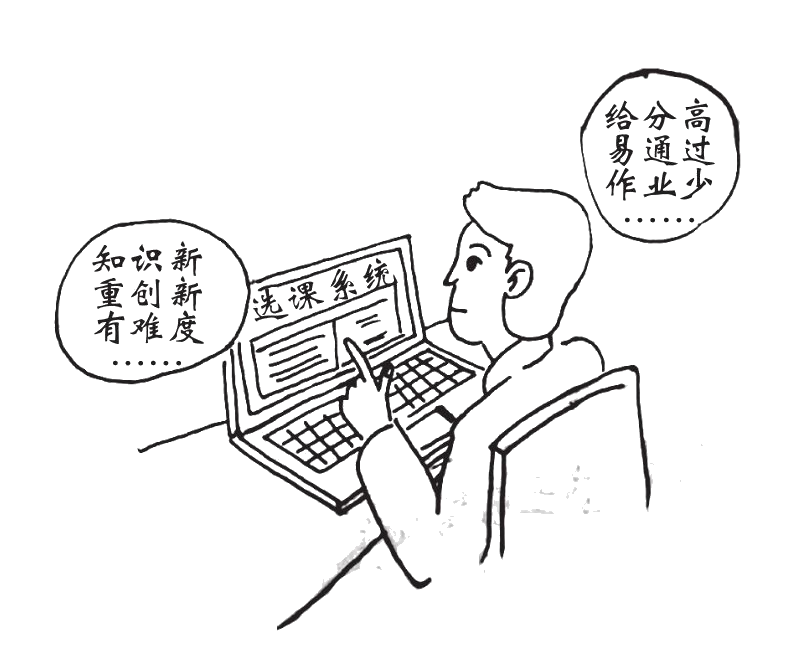
\includegraphics[width=0.53\linewidth]{picture/2018.png}
	\caption*{选课进行时}
\end{figure}



\checkpagenumber%
\bta{2019}

\section{Use of English}

\noindent
\textbf{Directions:}\\
Read the following text. Choose the best word(s) for each
numbered blank and mark A, B, C or D on the ANSWER SHEET. (10 points)



\TiGanSpace

Today we live in a world where GPS systems, digital maps, and
other navigation apps are available on our smartphones. \cloze of us just
walk straight into the woods without a phone. But phones  \cloze  on batteries,
and batteries can die faster than we realize.  \cloze  you get lost without a
phone or a compass, and you  \cloze  can't find north, we have a few tricks to
help you navigate  \cloze  to civilization, one of which is to follow the land.


When you find yourself  \cloze  a trail, but not in a completely  \cloze  area of land,
you have to answer two questions: Which  \cloze  is downhill, in this
particular area? And where is the nearest water source? Humans
overwhelmingly live in valleys, and on supplies of fresh water.  \cloze , if
you head downhill, and follow any H\textsubscript{2}O you find, you should  \cloze  see signs
of people. 

If you've explored the area before, keep an eye out for
familiar sights---you may be  \cloze  how quickly identifying a distinctive
rock or tree can restore your bearings.

 Another  \cloze  : Climb high
and look for signs of human habitation.  \cloze  , even in dense forest, you
should be able to  \cloze  gaps in the tree line due to roads, train tracks,
and other paths people carve  \cloze  the woods. Head toward these  \cloze  to find
a way out. At night, scan the horizon for  \cloze  light sources, such as
fires and streetlights, then walk toward the glow of light pollution.

 \cloze  , assuming you're lost in an area humans tend to frequent,
look for the  \cloze  we leave on the landscape. Trail blazes, tire tracks,
and other features can  \cloze  you to civilization.

\newpage

\begin{enumerate}
	%\renewcommand{\labelenumi}{\arabic{enumi}.}
	% A(\Alph) a(\alph) I(\Roman) i(\roman) 1(\arabic)
	%设定全局标号series=example	%引用全局变量resume=example
	%[topsep=-0.3em,parsep=-0.3em,itemsep=-0.3em,partopsep=-0.3em]
	%可使用leftmargin调整列表环境左边的空白长度 [leftmargin=0em]
	\item
\fourchoices
{Some}
{Most}
{Few}
{All}



\item

\fourchoices
{put}
{take}
{run}
{come}



\item

\fourchoices
{Since}
{If}
{Though}
{Until}




\item

\fourchoices
{formally}
{relatively}
{gradually}
{literally}



\item

\fourchoices
{back}
{next}
{around}
{away}



\item

\fourchoices
{onto}
{off}
{across}
{along}



\item

\fourchoices
{unattractive}
{uncrowded}
{unchanged}
{unfamiliar}


\item

\fourchoices
{site}
{point}
{way}
{place}



\item

\fourchoices
{So}
{Yet}
{Instead}
{Besides}




\item

\fourchoices
{immediately}
{intentionally}
{unexpectedly}
{eventually}




\item

\fourchoices
{surprised}
{annoyed}
{frightened}
{confused}



\item

\fourchoices
{problem}
{option}
{view}
{result}



\item

\fourchoices
{Above all}
{In contrast}
{On average}
{For example}



\item

\fourchoices
{bridge}
{avoid}
{spot}
{separate}



\item

\fourchoices
{from}
{through}
{beyond}
{under}


\item

\fourchoices
{posts}
{links}
{shades}
{breaks}


\item
\fourchoices
{artificial}
{mysterious}
{hidden}
{limited}


\item
\fourchoices
{Finally}
{Consequently}
{Incidentally}
{Generally}


\item

\fourchoices
{memories}
{marks}
{notes}
{belongings}


\item

\fourchoices
{restrict}
{adapt}
{lead}
{expose}

\end{enumerate}


\vfil

\section{Reading Comprehension}

\noindent
\textbf{Part A}\\
\textbf{Directions:}\\
 Read the following four texts. Answer the questions
after each text by choosing A, B, C or
D. Mark your answers on the
ANSWER SHEET. (40 points)

\newpage

\subsection{Text 1}

Financial regulators in Britain have imposed a rather unusual rule
on the bosses of big banks. Starting next year, any guaranteed bonus of
top executives could be delayed 10 years if their banks are under
investigation for wrongdoing. The main purpose of this ``clawback'' rule
is to hold bankers accountable for harmful risk-taking and to restore
public trust in financial institutions. Yet officials also hope for a
much larger benefit: more long-term decision-making, not only by banks
but by all corporations, to build a stronger economy for future
generations. 

``Short-termism,'' or the desire for quick profits,
has worsened in publicly traded companies, says the Bank of England's
top economist, Andrew Haldane. He quotes a giant of classical economics,
Alfred Marshall, in describing this financial impatience as acting like
``children who pick the plums out of their pudding to eat them at once''
rather than putting them aside to be eaten last. 



The average time
for holding a stock in both the United States and Britain, he notes, has
dropped from seven years to seven months in recent decades. Transient
investors, who demand high quarterly profits from companies, can hinder
a firm's efforts to invest in long-term research or to build up customer
loyalty. This has been dubbed ``quarterly capitalism.'' 


In addition, new digital technologies have allowed more rapid trading of
equities, quicker use of information, and thus shorter attention spans
in financial markets. ``There seems to be a predominance of short-term
thinking at the expense of long-term investing,'' said Commissioner
Daniel Gallagher of the US Securities and Exchange Commission in a
speech this week. 


In the US, \emph{the Sarbanes-Oxley Act of 2002} has
pushed most public companies to defer performance bonuses for senior
executives by about a year, slightly helping reduce ``short-termism.''
In its latest survey of CEO pay, \emph{The Wall Street Journal} finds that ``a
substantial part'' of executive pay is now tied to performance.




Much more could be done to encourage ``long-termism,'' such as
changes in the tax code and quicker disclosure of stock acquisitions. In
France, shareholders who hold onto a company investment for at least two
years can sometimes earn more voting rights in a company. 


Within companies, the right compensation design can provide incentives for
executives to think beyond their own time at the company and on behalf
of all stakeholders. Britain's new rule is a reminder to bankers that
society has an interest in their performance, not just for the short
term but for the long term.

\begin{enumerate}[resume]
	%\renewcommand{\labelenumi}{\arabic{enumi}.}
	% A(\Alph) a(\alph) I(\Roman) i(\roman) 1(\arabic)
	%设定全局标号series=example	%引用全局变量resume=example
	%[topsep=-0.3em,parsep=-0.3em,itemsep=-0.3em,partopsep=-0.3em]
	%可使用leftmargin调整列表环境左边的空白长度 [leftmargin=0em]
	\item
According to Paragraph 1, one motive in imposing the new rule is to \lineread.

\fourchoices
{enhance bankers' sense of responsibility}
{help corporations achieve larger profits}
{build a new system of financial regulation}
{guarantee the bonuses of top executives}


\item
Alfred Marshall is quoted to indicate \lineread.

\fourchoices
{the conditions for generating quick profits}
{governments' impatience in decision-making}
{the solid structure of publicly traded companies}
{``short-termism'' in economic activities}


\item
 It is argued that the influence of transient investment on public
companies can be \lineread.


\fourchoices
{indirect}
{adverse}
{minimal}
{temporary}



\item
The US and France examples are used to illustrate \lineread.


\fourchoices
{the obstacles to preventing ``short-termism''}
{the significance of long-term thinking}
{the approaches to promoting ``long-termism''}
{the prevalence of short-term thinking}


\item
Which of the following would be the best title for the text?

\fourchoices
{Failure of Quarterly Capitalism}
{Patience as a Corporate Virtue}
{Decisiveness Required of Top Executives}
{Frustration of Risk-taking Bankers}


\end{enumerate}



\newpage


\subsection{Text 2}

Grade inflation---the gradual increase in average GPAs
(grade-point averages) over the past few decades---is often considered
a product of a consumer era in higher education, in which students are
treated like customers to be pleased. But another, related force---a
policy often buried deep in course catalogs called ``grade forgiveness''---is helping raise GPAs. 


Grade forgiveness allows students to
retake a course in which they received a low grade, and the most recent
grade or the highest grade is the only one that counts in calculating a
student's overall GPA. 



The use of this little-known practice has
accelerated in recent years, as colleges continue to do their utmost to
keep students in school (and paying tuition) and improve their
graduation rates. When this practice first started decades ago, it was
usually limited to freshmen, to give them a second chance to take a
class in their first year if they struggled in their transition to
college-level courses. But now most colleges, save for many selective
campuses, allow all undergraduates, and even graduate students, to get
their low grades forgiven. 


College officials tend to emphasize
that the goal of grade forgiveness is less about the grade itself and
more about encouraging students to retake courses critical to their
degree program and graduation without incurring a big penalty.
``Ultimately,'' said Jack Miner, Ohio State University's registrar, ``we
see students achieve more success because they retake a course and do
better in subsequent courses or master the content that allows them to
graduate on time.'' 



That said, there is a way in which grade
forgiveness satisfies colleges' own needs as well. For public
institutions, state funds are sometimes tied partly to their success on
metrics such as graduation rates and student retention---so better
grades can, by boosting figures like those, mean more money. And
anything that raises GPAs will likely make students -- who, at the end
of the day, are paying the bill---feel they've gotten a better value
for their tuition dollars, which is another big concern for colleges.



Indeed, grade forgiveness is just another way that universities
are responding to consumers' expectations for higher education. Since
students and parents expect a college degree to lead to a job, it is in
the best interest of a school to turn out graduates who are as qualified
as possible---or at least appear to be. On this, students' and
colleges' incentives seem  \uline{to be aligned}.


\begin{enumerate}[resume]
	%\renewcommand{\labelenumi}{\arabic{enumi}.}
	% A(\Alph) a(\alph) I(\Roman) i(\roman) 1(\arabic)
	%设定全局标号series=example	%引用全局变量resume=example
	%[topsep=-0.3em,parsep=-0.3em,itemsep=-0.3em,partopsep=-0.3em]
	%可使用leftmargin调整列表环境左边的空白长度 [leftmargin=0em]
	\item
 What is commonly regarded as the cause of grade inflation?
\fourchoices
{The change of course catalogs.}
{Students' indifference to GPAs.}
{Colleges' neglect of GPAs.}
{The influence of consumer culture.}



\item
What was the original purpose of grade forgiveness?
\fourchoices
{To help freshmen adapt to college learning.}
{To maintain colleges' graduation rates.}
{To prepare graduates for a challenging future.}
{To increase universities' income from tuition.}


\item
 According to Paragraph 5, grade forgiveness enables colleges to \lineread.

\fourchoices
{obtain more financial support}
{boost their student enrollments}
{improve their teaching quality}
{meet local governments' needs}



\item
What does the phrase ``to be aligned'' (Line 5, Para. 6) most
probably mean?


\fourchoices
{To counterbalance each other.}
{To complement each other.}
{To be identical with each other.}
{To be contradictory to each other.}



\item
The author examines the practice of grade forgiveness by \lineread.

\fourchoices
{assessing its feasibility}
{analyzing the causes behind it}
{comparing different views on it}
{listing its long-run effects}

\end{enumerate}

\newpage

\subsection{Text 3}

This year marks exactly two centuries since the publication of
\emph{Frankenstein; or, The Modern Prometheus}, by Mary Shelley. Even
before the invention of the electric light bulb, the author produced a
remarkable work of speculative fiction that would foreshadow many
ethical questions to be raised by technologies yet to come. 


Today the rapid growth of artificial intelligence (AI) raises fundamental
questions: ``What is intelligence, identity, or consciousness? What
makes humans humans?'' 


What is being called artificial general
intelligence, machines that would imitate the way humans think,
continues to evade scientists. Yet humans remain fascinated by the idea
of robots that would look, move, and respond like humans, similar to
those recently depicted on popular sci-fi TV series such as
``Westworld'' and ``Humans''. 



Just how people think is still far too
complex to be understood, let alone reproduced, says David Eagleman, a
Stanford University neuroscientist. ``We are just in a situation where
there are no good theories explaining what consciousness actually is and
how you could ever build a machine to get there.'' 


But that doesn't
mean crucial ethical issues involving AI aren't at hand. The coming use
of autonomous vehicles, for example, poses thorny ethical questions.
Human drivers sometimes must make split-second decisions. Their
reactions may be a complex combination of instant reflexes, input from
past driving experiences, and what their eyes and ears tell them in that
moment. AI ``vision'' today is not nearly as sophisticated as that of
humans. And to anticipate every imaginable driving situation is a
difficult programming problem. 


Whenever decisions are based on
masses of data, ``you quickly get into a lot of ethical questions,''
notes Tan Kiat How, chief executive of a Singapore-based agency that is
helping the government develop a voluntary code for the ethical use of
AI. Along with Singapore, other governments and mega-corporations are
beginning to establish their own guidelines. Britain is setting up a
data ethics center. India released its AI ethics strategy this spring.



On June 7 Google pledged not to ``design or deploy AI'' that would
cause ``overall harm,'' or to develop AI-directed weapons or use AI for
surveillance that would violate international norms. It also pledged not
to deploy AI whose use would violate international laws or human rights.



While the statement is vague, it represents one starting point. So
does the idea that decisions made by AI systems should be explainable,
transparent, and fair. 


To put it another way: How can we make sure
that the thinking of intelligent machines reflects humanity's highest
values? Only then will they be useful servants and not Frankenstein's
out-of-control monster.


\begin{enumerate}[resume]
	%\renewcommand{\labelenumi}{\arabic{enumi}.}
	% A(\Alph) a(\alph) I(\Roman) i(\roman) 1(\arabic)
	%设定全局标号series=example	%引用全局变量resume=example
	%[topsep=-0.3em,parsep=-0.3em,itemsep=-0.3em,partopsep=-0.3em]
	%可使用leftmargin调整列表环境左边的空白长度 [leftmargin=0em]
	\item
Mary Shelley's novel \emph{Frankenstein} is mentioned because it \lineread.

\fourchoices
{fascinates AI scientists all over the world}
{has remained popular for as long as 200 years}
{involves some concerns raised by AI today}
{has sparked serious ethical controversies}



\item
In David Eagleman's opinion, our current knowledge of consciousness \lineread.

\fourchoices
{helps explain artificial intelligence}
{can be misleading to robot making}
{inspires popular sci-fi TV series}
{is too limited for us to reproduce it}


\item
The solution to the ethical issues brought by autonomous vehicles \lineread.

\fourchoices
{can hardly ever be found}
{is still beyond our capacity}
{causes little public concern}
{has aroused much curiosity}


\item
The author's attitude toward Google's pledges is one of \lineread.


\fourchoices
{affirmation}
{skepticism}
{contempt}
{respect}




\item
Which of the following would be the best title for the text?

\fourchoices
{AI's Future: In the Hands of Tech Giants}
{\emph{Frankenstein}, the Novel Predicting the Age of AI}
{The Conscience of AI: Complex But Inevitable}
{AI Shall Be Killers Once Out of Control}

\end{enumerate}


\newpage

\subsection{Text 4}





States will be able to force more people to pay sales tax when
they make online purchases under a Supreme Court decision Thursday that
will leave shoppers with lighter wallets but is a big financial win for
states. 


The Supreme Court's opinion Thursday overruled a pair of
decades-old decisions that states said cost them billions of dollars in
lost revenue annually. The decisions made it more difficult for states
to collect sales tax on certain online purchases. 


The cases the
court overturned said that if a business was shipping a customer's
purchase to a state where the business didn't have a physical presence
such as a warehouse or office, the business didn't have to collect sales
tax for the state. Customers were generally responsible for paying the
sales tax to the state themselves if they weren't charged it, but most
didn't realize they owed it and few paid. 


Justice Anthony Kennedy
wrote that the previous decisions were flawed. ``Each year the physical
presence rule becomes further removed from economic reality and results
in significant revenue losses to the States,'' he wrote in an opinion
joined by four other justices. Kennedy wrote that the rule ``limited
states' ability to seek long-term prosperity and has prevented market
participants from competing on an even playing field.'' 


The ruling
is a victory for big chains with a presence in many states, since they
usually collect sales tax on online purchases already. Now, rivals will
be charging sales tax where they hadn't before. Big chains have been
collecting sales tax nationwide because they typically have physical
stores in whatever state a purchase is being shipped to. Amazon.com,
with its network of warehouses, also collects sales tax in every state
that charges it, though third-party sellers who use the site don't have
to. 



Until now, many sellers that have a physical presence in only
a single state or a few states have been able to avoid charging sales
taxes when they ship to addresses outside those states. Sellers that use
eBay and Etsy, which provide platforms for smaller sellers, also haven't
been collecting sales tax nationwide. Under the ruling Thursday, states
can pass laws requiring out-of-state sellers to collect the state's
sales tax from customers and send it to the state.


 Retail trade
groups praised the ruling, saying it levels the playing field for local
and online businesses. The losers, said retail analyst Neil Saunders,
are online-only retailers, especially smaller ones. Those retailers may
face headaches complying with various state sales tax laws. The Small
Business \& Entrepreneurship Council advocacy group said in a statement,
``Small businesses and internet entrepreneurs are not well served at all
by this decision.''

\begin{enumerate}[resume]
	%\renewcommand{\labelenumi}{\arabic{enumi}.}
	% A(\Alph) a(\alph) I(\Roman) i(\roman) 1(\arabic)
	%设定全局标号series=example	%引用全局变量resume=example
	%[topsep=-0.3em,parsep=-0.3em,itemsep=-0.3em,partopsep=-0.3em]
	%可使用leftmargin调整列表环境左边的空白长度 [leftmargin=0em]
	\item
The Supreme Court decision Thursday will \lineread.


\fourchoices
{better businesses' relations with states}
{put most online businesses in a dilemma}
{make more online shoppers pay sales tax}
{force some states to cut sales tax}

\item
It can be learned from paragraphs 2 and 3 that the overruled
decisions \lineread.


\fourchoices
{have led to the dominance of e-commerce}
{have cost consumers a lot over the years}
{were widely criticized by online purchasers}
{were considered unfavorable by states}


\item
According to Justice Anthony Kennedy, the physical presence rule has \lineread.



\fourchoices
{hindered economic development}
{brought prosperity to the country}
{harmed fair market competition}
{boosted growth in states' revenue}



\item
Who are most likely to welcome the Supreme Court ruling?

\fourchoices
{Internet entrepreneurs.}
{Big-chain owners.}
{Third-party sellers.}
{Small retailers.}



\item
In dealing with the Supreme Court decision Thursday, the author \lineread.

\fourchoices
{gives a factual account of it and discusses its consequences}
{describes the long and complicated process of its making}
{presents its main points with conflicting views on them}
{cites some cases related to it and analyzes their implications}

\end{enumerate}



\newpage

\noindent
\textbf{Part B}\\
\textbf{Directions:}\\
 The following paragraphs are given in a wrong order.
For Questions 41-45, you are required to reorganize these paragraphs
into a coherent text by choosing from the list A-G and filling them into
the numbered boxes. Paragraphs C and F have been correctly placed. Mark
your answers on the ANSWER SHEET. (10 points)


\begin{listmatch}
\item 
These tools can help you win every argument---not in the
unhelpful sense of beating your opponents but in the better sense of
learning about the issues that divide people. Learning why they disagree
with us and learning to talk and work together with them. If we readjust
our view of arguments---from a verbal fight or tennis game to a
reasoned exchange through which we all gain mutual respect, and
understanding---then we change the very nature of what it means to
``win'' an argument.


\item 
 Of course, many discussions are not so successful. Still, we need
to be careful not to accuse opponents of bad arguments too quickly. We
need to learn how to evaluate them properly. A large part of evaluation
is calling out bad arguments, but we also need to admit good arguments
by opponents and to apply the same critical standards to ourselves.
Humility requires you to recognize weakness in your own arguments and
sometimes also to accept reasons on the opposite side.


\item 
None of these will be easy but you can start even if others
refuse to. Next time you state your position, formulate an argument for
what you claim and honestly ask yourself whether your argument is any
good. Next time you talk with someone who takes a stand, ask them to
give you a reason for their view. Spell out their argument fully and
charitably. Assess its strength impartially. Raise objections and listen
carefully to their replies.


\item 
Carnegie would be right if arguments were fights, which is how we
often think of them. Like physical fights, verbal fights can leave both
sides bloodied. Even when you win, you end up no better off. Your
prospects would be almost as dismal if arguments were even just
competitions---like, say, tennis games. Pairs of opponents hit the ball back and forth until one winner emerges from
all who entered. Everybody else loses. This kind of thinking is why so
many people try to avoid arguments, especially about politics and
religion.


\item 
 In his 1936 work \emph{How to Win Friends and Influence People}, Dale
Carnegie wrote: ``There is only one way\ldots to get the best of an
argument---and that is to avoid it.'' This aversion to arguments is
common, but it depends on a mistaken view of arguments that causes
profound problems for our personal and social lives---and in many ways
misses the point of arguing in the first place.


\item 
These views of arguments also undermine reason. If you see a
conversation as a fight or competition, you can win by cheating as long
as you don't get caught. You will be happy to convince people with bad
arguments. You can call their views stupid, or joke about how ignorant
they are. None of these tricks will help you understand them, their
positions or the issues that divide you, but they can help you win---in
one way.


\item 
There is a better way to win arguments. Imagine that you favor
increasing the minimum wage in our state, and I do not. If you yell,
``Yes,'' and I yell, ``No,'' neither of us learns anything. We neither
understand nor respect each other, and we have no basis for compromise
or cooperation. In contrast, suppose you give a reasonable argument:
that full-time workers should not have to live in poverty. Then I
counter with another reasonable argument: that a higher minimum wage
will force businesses to employ fewer people for less time. Now we can
understand each other's positions and recognize our shared values, since
we both care about needy workers.

\end{listmatch}



\[ 
\begin{tabular}{|c|c|}
	\hline
	41. &  \hspace{1.5em} \\
	\hline
\end{tabular}
\rightarrow
\begin{tabular}{|c|c|}
	\hline
	42. &  \hspace{1.5em} \\
	\hline
\end{tabular}
\rightarrow
\begin{tabular}{|c|}
	\hline
	F \\
	\hline
\end{tabular}
\rightarrow
\begin{tabular}{|c|c|}
	\hline
	43. &  \hspace{1.5em} \\
	\hline
\end{tabular}
\rightarrow
\begin{tabular}{|c|c|}
	\hline
	44. &  \hspace{1.5em} \\
	\hline
\end{tabular}
\rightarrow
\begin{tabular}{|c|}
	\hline
	C \\
	\hline
\end{tabular}
\rightarrow
\begin{tabular}{|c|c|}
	\hline
	45. &  \hspace{1.5em} \\
	\hline
\end{tabular}
\]


\phantom{ \linefill \linefill \linefill \linefill \linefill}


\newpage

\noindent
\textbf{Part C}\\
\textbf{Directions:}\\
 Read the following text carefully and then translate
the underlined segments into Chinese. Write your answers on the ANSWER SHEET. (10 points)


\TiGanSpace


It was only after I started to write a weekly column about the
medical journals, and began to read scientific papers from beginning to
end, that I realised just how bad much of the medical literature
frequently was. I came to recognise various signs of a bad paper: the
kind of paper that purports to show that people who eat more than one
kilo of broccoli a week were 1.17 times more likely than those who eat
less to suffer late in life from pernicious anaemia. \transnum \uline{There is a
great deal of this kind of nonsense in the medical journals which, when
taken up by broadcasters and the lay press, generates both health scares
and short-lived dietary enthusiasms. }



Why is so much bad science
published? A recent paper, titled ``The Natural Selection of Bad
Science'', published on the Royal Society's open science website,
attempts to answer this intriguing and important question. It says that
the problem is not merely that people do bad science, but that our
current system of career advancement positively encourages it. What is
important is not truth, but publication, which has become almost an end
in itself. There has been a kind of inflationary process at work: \transnum \uline{nowadays anyone applying for a research post has to have published twice
the number of papers that would have been required for the same post
only 10 years ago. Never mind the quality, then, count the number.}



\transnum \uline{Attempts have been made to curb this tendency, for example,
by trying to incorporate some measure of quality as well as quantity
into the assessment of an applicant's papers.} This is the famed citation
index, that is to say the number of times a paper has been quoted
elsewhere in the scientific literature, the assumption being that an
important paper will be cited more often than one of small account. \transnum \uline{This would be reasonable if it were not for the fact that scientists can
easily arrange to cite themselves in their future publications, or get
associates to do so for them in return for similar favours.}



Boiling down an individual's output to simple metrics, such as
number of publications or journal impacts, entails considerable savings
in time, energy and ambiguity. Unfortunately, the long-term costs of
using simple quantitative metrics to assess researcher merit are likely
to be quite great. \transnum \uline{If we are serious about ensuring that our
science is both meaningful and reproducible, we must ensure that our
institutions encourage that kind of science.}



\newpage

\section{Writing}

\noindent
\textbf{Part A}\\
\textbf{51. Directions:} 
 
 Suppose you are working for the ``Aiding
Rural Primary School'' project of your university. Write an email to
answer the inquiry from an international student volunteer, specifying
the details of the project. 

You should write about 100 words on the
ANSWER SHEET. 

\textbf{Do not} use your own name in the email. Use ``Li Ming''
instead. (10 points)


\vspace{2em}

\noindent
\textbf{Part B}\\
\textbf{52. Directions:} 

Write an essay of 160-200 words based on the
picture below. In your essay, you should
\begin{listwrite}
	\item 
 describe the picture briefly,
\item 
interpret the implied meaning, and 
\item 
give your comments. 
\end{listwrite}

You should write neatly on the ANSWER SHEET. (20 points)


\begin{figure}[h!]
	\centering
	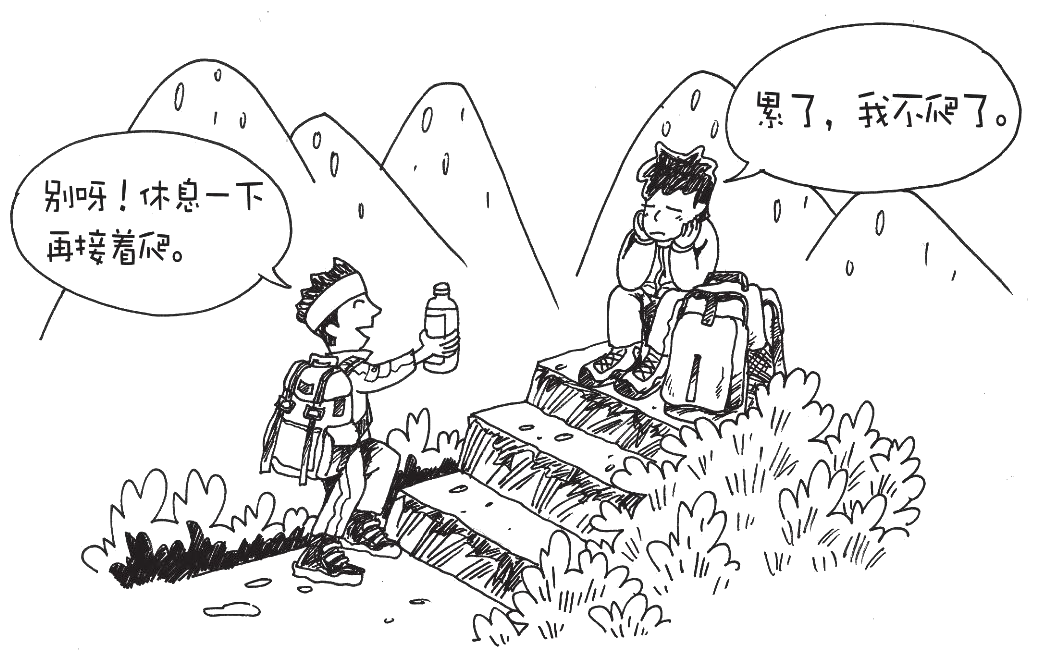
\includegraphics[width=0.58\linewidth]{picture/2019.png}
	\caption*{途中}
\end{figure}




%


\bta{2020}



\section{Use of English}

\noindent
\textbf{Directions:}\\
Read the following text. Choose the best word(s) for each numbered blank
and mark A, B, C or D on the ANSWER SHEET. (10 points)



\TiGanSpace


Even if families don't sit down to eat together as frequently as before,
millions of Britons will nonetheless have got a share this weekend of
one of that nation's great traditions: the Sunday roast. \cloze a
cold winter's day, few culinary pleasures can \cloze it. Yet as
we report now, the food police are determined that this \cloze
should be rendered yet another guilty pleasure \cloze to damage
our health.

The Food Standards Authority (FSA) has \cloze a public warning
about the risks of a compound called acrylamide that forms in some foods
cooked \cloze high temperatures. This means that people should
\cloze crisping their roast potatoes, reject thin-crust pizzas
and only \cloze toast their bread. But where is the evidence to
support such alarmist advice? \cloze studies have shown that
acrylamide can cause neurological damage in mice, there is no
\cloze evidence that it causes cancer in humans.

Scientists say the compound is \cloze to cause cancer but have
no hard scientific proof. \cloze the precautionary principle, it
could be argued that it is \cloze to follow the FSA advice.
\cloze , it was rumoured that smoking caused cancer for years
before the evidence was found to prove a \cloze.

Doubtless a piece of boiled beef can always be \cloze up on
Sunday alongside some steamed vegetables, without the Yorkshire pudding
and no wine. But would life be worth living? \cloze , the FSA
says it is not telling people to cut out roast foods \cloze , but
to reduce their lifetime intake. However, their \cloze risks
coming across as being pushy and overprotective. Constant health scares
just \cloze with no one listening.

\newpage
\begin{enumerate}
\item


\fourchoices
{In}
{On}
{Till}
{Towards}

\item


\fourchoices
{match}
{express}
{satisfy}
{influence}

\item


\fourchoices
{patience}
{concern}
{surprise}
{enjoyment}

\item

\fourchoices
{intensified}
{guaranteed}
{compelled}
{privileged}

\item


\fourchoices
{ignored}
{received}
{issued}
{cancelled}


\item


\fourchoices
{under}
{by}
{for}
{at}

\item


\fourchoices
{forget}
{avoid}
{finish}
{regret}

\item


\fourchoices
{easily}
{regularly}
{partially}
{initially}

\item


\fourchoices
{If}
{Since}
{While}
{Unless}



\item

\fourchoices
{conclusive}
{external}
{secondary}
{negative}



\item


\fourchoices
{likely}
{bound}
{insufficient}
{slow}




\item

\fourchoices
{In addition to}
{At the cost of}
{On the basis of}
{In contrast to}



\item

\fourchoices
{interesting}
{fortunate}
{urgent}
{advisable}



\item

\fourchoices
{As usual}
{After all}
{By definition}
{In particular}





\item

\fourchoices
{connection}
{combination}
{resemblance}
{pattern}



\item


\fourchoices
{made}
{used}
{saved}
{served}






\item

\fourchoices
{To be brief}
{For instance}
{To be fair}
{In general}


\item

\fourchoices
{entirely}
{gradually}
{reluctantly}
{carefully}



\item

\fourchoices
{promise}
{competition}
{experience}
{campaign}




\item


\fourchoices
{follow up}
{end up}
{open up}
{pick up}

\end{enumerate}

\vfil

\section{Reading Comprehension}




\noindent
\textbf{Part A}\\
\textbf{Directions:}\\
Read the following four texts. Answer the questions after each text by
choosing A, B, C or
D. Mark your answers on the ANSWER SHEET. (40
points)



\newpage
\subsection{Text 1}


A group of Labour MPs, among them Yvette Cooper, are bringing in the new
year with a call to institute a UK ``town of culture'' award. The
proposal is that it should sit alongside the existing city of culture
title, which was held by Hull in 2017, and has been awarded to Coventry
for 2021. Cooper and her colleagues argue that the success of the crown
for Hull, where it brought in £220m of investment and an avalanche of
arts, ought not to be confined to cities. Britain's towns, it is true,
are not prevented from applying, but they generally lack the resources
to put together a bid to beat their bigger competitors. A town of
culture award could, it is argued, become an annual event, attracting
funding and creating jobs.

Some might see the proposal as a booby prize for the fact that Britain
is no longer able to apply for the much more prestigious title of
European capital of culture, a sought-after award bagged by Glasgow in
1990 and Liverpool in 2008. A cynic might speculate that the UK is on
the verge of disappearing into an endless fever of self-celebration in
its desperation to reinvent itself for the post-Brexit world: after town
of culture, who knows what will follow---village of culture? Suburb of
culture? Hamlet of culture?


It is also wise to recall that such titles are not a cure-all. A badly
run ``year of culture'' washes in and washes out of a place like the
tide, bringing prominence for a spell but leaving no lasting benefits to
the community. The really successful holders of such titles are those
that do a great deal more than fill hotel bedrooms and bring in
high-profile arts events and good press for a year. They transform the
aspirations of the people who live there; they nudge the self-image of
the city into a bolder and more optimistic light. It is hard to get
right, and requires a remarkable degree of vision, as well as
cooperation between city authorities, the private sector, community
groups and cultural organisations. But it can be done: Glasgow's year as
European capital of culture can certainly be seen as one of a complex
series of factors that have turned the city into the powerhouse of art,
music and theatre that it remains today.

A ``town of culture'' could be not just about the arts but about
honouring a town's peculiarities---helping sustain its high street,
supporting local facilities and above all celebrating its people. Jeremy
Wright, the culture secretary, should welcome this positive, hope-filled
proposal, and turn it into action.


\begin{enumerate}[resume]
\item
Cooper and her colleagues argue that a ``town of culture'' award could  \lineread.




\fourchoices
{consolidate the town-city ties in Britain}
{promote cooperation-among Britain's towns}
{increase the economic strength of Britain's towns}
{focus Britain's limited resources on cultural events}



\item
 According to Paragraph 2, the proposal might be regarded by some as \lineread.


\fourchoices
{a sensible compromise}
{a self-deceiving attempt}
{an eye-catching bonus}
{an inaccessible target}



\item
The author suggests that a title holder is successful only if it \lineread.


\fourchoices
{endeavours to maintain its image}
{meets the aspiration of its people}
{brings its local arts to prominence}
{commits to its long-term growth}


\item
 Glasgow is mentioned in Paragraph 3 to present \lineread.


\fourchoices
{a contrasting case}
{a supporting example}
{a background story}
{a related topic}


\item
What is the author's attitude towards the proposal?


\fourchoices
{Skeptical.}
{Objective.}
{Favourable.}
{Critical.}


\end{enumerate}


\newpage
\subsection{Text 2}



Scientific publishing has long been a licence to print money. Scientists
need journals in which to publish their research, so they will supply
the articles without monetary reward. Other scientists perform the
specialised work of peer review also for free, because it is a central
element in the acquisition of status and the production of scientific
knowledge.

With the content of papers secured for free, the publisher needs only
find a market for its journal. Until this century, university libraries
were not very price sensitive. Scientific publishers routinely report
profit margins approaching 40\% on their operations, at a time when the
rest of the publishing industry is in an existential crisis.

The Dutch giant Elsevier, which claims to publish 25\% of the scientific
papers produced in the world, made profits of more than £900m last year,
while UK universities alone spent more than £210 m in 2016 to enable
researchers to access their own publicly funded research; both figures
seem to rise unstoppably despite increasingly desperate efforts to
change them.

The most drastic, an thoroughly illegal, reaction has been the emergence
of Sci-Hub, a kind of global photocopier for scientific papers, set up
in 2012, which now claims to offer access to every paywalled article
published since 2015. The success of Sci-Hub, which relies on
researchers passing on copies they have themselves legally accessed,
shows the legal ecosystem has lost legitimacy among its users and must
be transformed so that it works for all participants.

In Britain the move towards open access publishing has been driven by
funding bodies. In some ways it has been very successful. More than half
of all British scientific research is now published under open access
terms: either freely available from the moment of publication, or
paywalled for a year or more so that the publishers can make a profit
before being placed on general release.

Yet the new system has not yet worked out any cheaper for the
universities. Publishers have responded to the demand that they make
their product free to readers by charging their writers fees to cover
the costs of preparing an article. These range from around £500 to
\$5,000.  A report last year pointed out that the costs both of
subscriptions and of these ``article preparation costs'' had been
steadily rising at a rate above inflation.
In some ways the scientific publishing model resembles the economy of
the social internet: labour is provided free in exchange for the hope of
status, while huge profits are made by a few big firms who run the
market places. In both cases, we need a rebalancing of power.

\begin{enumerate}[resume]
	%\renewcommand{\labelenumi}{\arabic{enumi}.}
	% A(\Alph) a(\alph) I(\Roman) i(\roman) 1(\arabic)
	%设定全局标号series=example	%引用全局变量resume=example
	%[topsep=-0.3em,parsep=-0.3em,itemsep=-0.3em,partopsep=-0.3em]
	%可使用leftmargin调整列表环境左边的空白长度 [leftmargin=0em]
	\item
Scientific publishing is seen as ``a licence to print money'' partly
because \lineread.


\fourchoices
{its funding has enjoyed a steady increase}
{its marketing strategy has been successful}
{its payment for peer review is reduced}
{its content acquisition costs nothing}


\item
According to Paragraphs 2 and 3, scientific publishers Elsevier have \lineread.


\fourchoices
{thrived mainly on university libraries}
{gone through an existential crisis}
{revived the publishing industry}
{financed researchers generously}


\item
How does the author feel about the success of Sci-Hub?


\fourchoices
{Relieved.}
{Puzzled.}
{Concerned.}
{Encouraged.}


\item
 It can be learned from Paragraphs 5 and 6 that open access terms \lineread.


\fourchoices
{allow publishers some room to make money}
{render publishing much easier for scientists}
{reduce the cost of publication substantially}
{free universities from financial burdens}


\item
Which of the following characterizes the scientific publishing
model?


\fourchoices
{Trial subscription is offered.}
{Labour triumphs over status.}
{Costs are well controlled.}
{The few feed on the many.}


\end{enumerate}


\newpage
\subsection{Text 3}


Progressives often support diversity mandates as a path to equality and
a way to level the playing field. But all too often such policies are an
insincere form of virtue-signaling that benefits only the most
privileged and does little to help average people.

A pair of bills sponsored by Massachusetts state Senator Jason Lewis and
House Speaker Pro Tempore Patricia Haddad, to ensure ``gender parity''
on boards and commissions, provide a case in point.


Haddad and Lewis are concerned that more than half the state-government
boards are less than 40 percent female. In order to ensure that elite
women have more such opportunities, they have proposed imposing
government quotas. If the bills become law, state boards and commissions
will be required to set aside 50 percent of board seats for women by 2022.

The bills are similar to a measure recently adopted in Califomia, which
last year became the first state to require gender quotas for private
companies. In signing the measure, California Governor Jerry Brown
admitted that the law, which expressly classifies people on the basis of
sex, is probably unconstitutional.

The US Supreme Court frowns on sex-based classifications unless they are
designed to address an ``important'' policy interest, Because the
California law applies to all boards, even where there is no history of
prior discrimination, courts are likely to rule that the law violates
the constitutional guarantee of ``equal protection''.

But are such government mandates even necessary? Female participation on
corporate boards may not currently mirror the percentage of women in the
general population, but so what?

The number of women on corporate boards has been steadily increasing
without government interference. According to a study by Catalyst,
between 2010 and 2015 the share of women on the boards of global
corporations increased by 54 percent.

Requiring companies to make gender the primary qualification for board
membership will inevitably lead to less experienced private sector
boards. That is exactly what happened when Norway adopted a nationwide
corporate gender quota.

Writing in \emph{The New Republic}, Alice Lee notes that increasing the
number of opportunities for board membership without increasing the pool
of qualified women to serve on such boards has led to a ``golden skirt''
phenomenon, where the same elite women scoop up multiple seats on a
variety of boards.

Next time somebody pushes corporate quotas as a way to promote gender
equity, remember that such policies are largely self-serving measures
that make their sponsors feelgood but do little to help average women.


\begin{enumerate}[resume]
	%\renewcommand{\labelenumi}{\arabic{enumi}.}
	% A(\Alph) a(\alph) I(\Roman) i(\roman) 1(\arabic)
	%设定全局标号series=example	%引用全局变量resume=example
	%[topsep=-0.3em,parsep=-0.3em,itemsep=-0.3em,partopsep=-0.3em]
	%可使用leftmargin调整列表环境左边的空白长度 [leftmargin=0em]
	\item
The author believes that the bills sponsored by Lewis and Haddad will \lineread.


\fourchoices
{help little to reduce gender bias}
{pose a threat to the state government}
{raise women's position in politics}
{greatly broaden career options}


\item
 Which of the following is true of the Califormia measure?


\fourchoices
{It has irritated private business owners.}
{It is welcomed by the Supreme Court.}
{It may go against the Constitution.}
{It will settle the prior controversies.}


\item
 The author mentions the study by Catalyst to illustrate \lineread.


\fourchoices
{the harm from arbitrary board decision}
{the importance of constitutional guarantees}
{the pressure on women in global corporations}
{the needlessness of government interventions}


\item
Norway's adoption of a nationwide corporate gender quota has led to \lineread.


\fourchoices
{the underestimation of elite women's role}
{the objection to female participation on boards}
{the entry of unqualified candidates into the board}
{the growing tension between labor and management}



\item
 Which of the following can be inferred from the text?


\fourchoices
{Women's need in employment should be considered.}
{Feasibility should be a prime concern in policymaking.}
{Everyone should try hard to promote social justice.}
{Major social issues should be the focus of legislation.}

\end{enumerate}



\newpage
\subsection{Text 4}


Last Thursday, the French Senate passed a digital services tax, which
would impose an entirely new tax on large multinationals that provide
digital services to consumers or users in France. Digital services
include everything from providing a platform for selling goods and
services online to targeting advertising based on user data, and the tax
applies to gross revenue from such services. Many French politicians and
media outlets have referred to this as a `` GAFA tax,'' meaning that it
is designed to apply primarily to companies such as Google, Apple,
Facebook and Amazon---in other words, multinational tech companies based
in the United States.

The digital services tax now awaits the signature of President Emmanuel
Macron, who has expressed support for the measure, and it could go into
effect within the next few weeks. But it has already sparked significant
controversy, with the United States trade representative opening an
investigation into whether the tax discriminates against American
companies, which in tum could lead to trade sanctions against France.

The French tax is not just a unilateral move by one country in need of
revenue.
Instead, the digital services tax is part of a much larger trend, with
countries over the past few years proposing or putting in place an
alphabet soup of new international tax provisions. They have included
Britain's DPT. (diverted profits tax), Australia's MAAL (multinational
anti-avoidance law), and India's SEP (significant economic presence)
test, to name but a few. At the same time, the European Union, Spain,
Britain and several other countries have all seriously contemplated
digital services taxes.

These unilateral developments differ in their specifics, but they are
all designed to tax multinationals on income and revenue that countries
believe they should have a right to tax, even if international tax rules
do not grant them that right. In other words, they all share a view that
the international tax system has failed to keep up with the current
economy.

In response to these many unilateral measures, the Organization for
Economic Cooperation and Development (OECD) is currently working with
131 countries to reach a consensus by the end of 2020 on an
international solution. Both France and the United States are involved
in the organization's work, but France's digital services tax and the
American response raise questions about what the future holds for the
international tax system.

France's planned tax is a clear warning: Unless a broad consensus can be
reached on reforming the international tax system, other nations are
likely to follow suit, and American companies will face a cascade of
different taxes from dozens of nations that will prove burdensome and
costly.

\begin{enumerate}[resume]
	%\renewcommand{\labelenumi}{\arabic{enumi}.}
	% A(\Alph) a(\alph) I(\Roman) i(\roman) 1(\arabic)
	%设定全局标号series=example	%引用全局变量resume=example
	%[topsep=-0.3em,parsep=-0.3em,itemsep=-0.3em,partopsep=-0.3em]
	%可使用leftmargin调整列表环境左边的空白长度 [leftmargin=0em]
	\item
The French Senate has passed a bill to \lineread.


\fourchoices
{regulate digital services platforms}
{protect French companies'' interests}
{impose a levy on tech multinationals}
{curb the influence of advertising}


\item
It can be learned from Paragraph 2 that the digital services tax \lineread.


\fourchoices
{may trigger countermeasures against France}
{is apt to arouse criticism at home and abroad}
{aims to ease international trade tensions}
{will prompt the tech giants to quit France}


\item
The countries adopting the unilateral measures share the opinion
that \lineread.


\fourchoices
{redistribution of tech giants' revenue must be ensured}
{the current international tax system needs upgrading}
{tech multinationals' monopoly should be prevented}
{all countries ought to enjoy equal taxing rights}


\item
It can be learned from Paragraph 5 that the OECD's current work \lineread.


\fourchoices
{is being resisted by US companies}
{needs to be readjusted immediately}
{is faced with uncertain prospects}
{needs to in involve more countries}


\item
Which of the following might be the best title for this text?


\fourchoices
{France Is Confronted with Trade Sanctions}
{France leads the charge on Digital Tax}
{France Says ``NO'' to Tech Multinationals}
{France Demands a Role in the Digital Economy}


\end{enumerate}

\newpage
\noindent
\textbf{Part B}\\
\textbf{Directions:}\\
Read the following text and answer the questions by choosing the most
suitable subheading from the list A-G for each of the numbered
paragraphs (41-45). There are two extra subheadings. Mark your answers
on the ANSWER SHEET. (10 points)


\begin{listmatch}
\item 
Eye fixations are brief


\item 
Too much eye contact is instinctively felt to be rude


\item 
Eye contact can be a friendly social signal


\item 
Personality can affect how a person reacts to eye contact


\item 
Biological factors behind eye contact are being investigated


\item 
Most people are not comfortable holding eye contact with
strangers


\item 
Eye contact can also be aggressive.
\end{listmatch}




In a social situation, eye contact with another person can show that you
are paying attention in a friendly way. But it can also be antagonistic
such as when a political candidate turns toward their competitor during
a debate and makes eye contact that signals hostility. Here's what hard
science reveals about eye contact:

\linefill.

We know that a typical infant will instinctively gaze into its mother's
eyes, and she will look back. This mutual gaze is a major part of the
attachment between mother and child. In adulthood, looking someone else
in a pleasant way can be a complimentary sign of paying attention. It
can catch someone's attention in a crowded room, ``Eye contact and
smile'' can signal availability and confidence, a common-sense notion
supported in studies by psychologist Monica Moore.

\linefill.

Neuroscientist Bonnie Auyeung found that the hormone oxytocin increased
the amount of eye contact from men toward the interviewer during a brief
interview when the direction of their gaze was recorded. This was also
found in high-functioning men with some autistic spectrum symptoms, who
may tend to avoid eye contact. Specific brain regions that respond
during direct gaze are being explored by other researches, using
advanced methods of brain scanning.


\linefill.

With the use of eye-tracking technology, Julia Minson of the Harvard
Kennedy School of Government concluded that eye contact can signal very
different kinds of messages, depending on the situation. While eye
contact may be a sign of connection or trust in friendly situations,
it's more likely to be associated with dominance or intimidation in
adversarial situations. ``Whether you're a politician or a parent, it
might be helpful to keep in mind that trying to maintain eye contact may
backfire if you're trying to convince someone who has a different set of
beliefs than you,''said Minson.


\linefill.

When we look at a face or a picture, our eyes pause on one spot at a
time, often on the eyes or mouth. These pauses typically occur at about
three per second, and the eyes then jump to another spot, until several
important points in the image are registered like a series of snapshots.
How the whole image is then assembled and perceived is still a mystery
although it is the subject of current research.


\linefill.

In people who score high in a test of neuroticism, a personality
dimension associated with self-consciousness and anxiety, eye contact
triggered more activity associated with avoidance, according to the
Finnish researcher Jari Hietanen and colleagues ``Our findings indicate
that people do not only feel different when they are the centre of
attention but that their brain reactions also differ.'' A more direct
finding is that people who scored highly for negative emotions like
anxiety looked at others for shorter periods of time and reported more
comfortable feelings when others did not look directly at them.


\newpage
\noindent
\textbf{Part C}\\
\textbf{Directions:}\\
Read the following text carefully and then translate the underlined
segments into Chinese.   Written your answer on the
ANSWER SHEET. (10 points)


\TiGanSpace

Following the explosion of creativity in Florence during the 14th
century known as the Renaissance, the modern world saw a departure from
what it had once known. It turned from God and the authority of the
Roman Catholic Church and instead favoured a more humanistic approach to
being. Renaissance ideas had spread throughout Europe well into the 17th
century, with the arts and sciences flourishing extraordinarily among
those with a more logical disposition. \transnum \uline{with the Church's
teachings and ways of thinking eclipsed by the Renaissance, the gap
between the Medieval and modern periods had been bridged leading to new
and unexplored intellectual territories.}

During the Renaissance, the great minds of Nicolaus Copernicus, Johannes
Kepler and Galileo Galilei demonstrated the power of scientific study
and discovery. \transnum \uline{Before each of their revelations many
thinkers at the time had sustained more ancient ways of thinking,
including the geocentric view that the Earth was at the centre of our
universe.} Copernicus theorized in 1543 that all of the planets that we
knew of revolved not around the Earth, but the Sun, a system that was
later upheld by Galileo at his own expense. Offering up such a theory
during a time of high tension between scientific and religious minds was
branded as heresy and any such heretics that continued to spread these
lies were to be punished by imprisonment or even death.


\transnum \uline{Despite attempts by the Church to suppress. this new
generation of logicians and rationalists, more explanations for how the
universe functioned were being made at a rate that the people could no
longer ignore}. It was with these great revelations that a new kind of
philosophy founded in reason was born.

The Church's long-standing dogma was losing the great battle for truth
to rationalists and scientists. This very fact embodied the new ways of
thinking that swept through Europe during most of 17th century. (49)
\uline{As many took on the duty of trying to integrate reasoning and
scientific philosophies into the world, the Renaissance was over and it
was time for a new era - the Age of Reason.}

The 17th and 18th centuries were times of radical change and curiosity,
Scientific method, reductionism and the questioning of Church ideals was
to be encouraged, as were ideas of liberty, tolerance and progress. (50)
\uline{Such actions to seek knowledge and to understand what
information we already knew were captured by the Latin phrase `sapere
aude' or `dare to know',} after Immanuel Kant used it in his essay
\emph{An Answer to the Question}: \emph{What is Enlightenment?}. It was
the purpose and responsibility of great minds to go forth and seek out
the truth, which they believed to be founded in knowledge.


\newpage
\section{Writing}



\noindent
\textbf{Part A}\\
\textbf{51. Directions:}


The Students Union of your university has assigned you to inform the
international students about an upcoming singing contest. Write a notice
in about 100 words.

Write your answer on the ANSWER SHEET.

\textbf{Do not} use your own name in the notice. (10 points)


\vspace{2em}

\noindent
\textbf{Part B}\\
\textbf{52. Directions:}



Write an essay of 160-200 words based on the picture below. In your
essay, you should

\begin{listwrite}
	\item 
	 describe the picture briefly,
	
	\item 
	 interpret the implied meaning, and
	
	\item 
	 give your comments.
\end{listwrite}


You should write neatly on the ANSWER SHEET. (20 points)


\begin{figure}[h!]
	\centering
	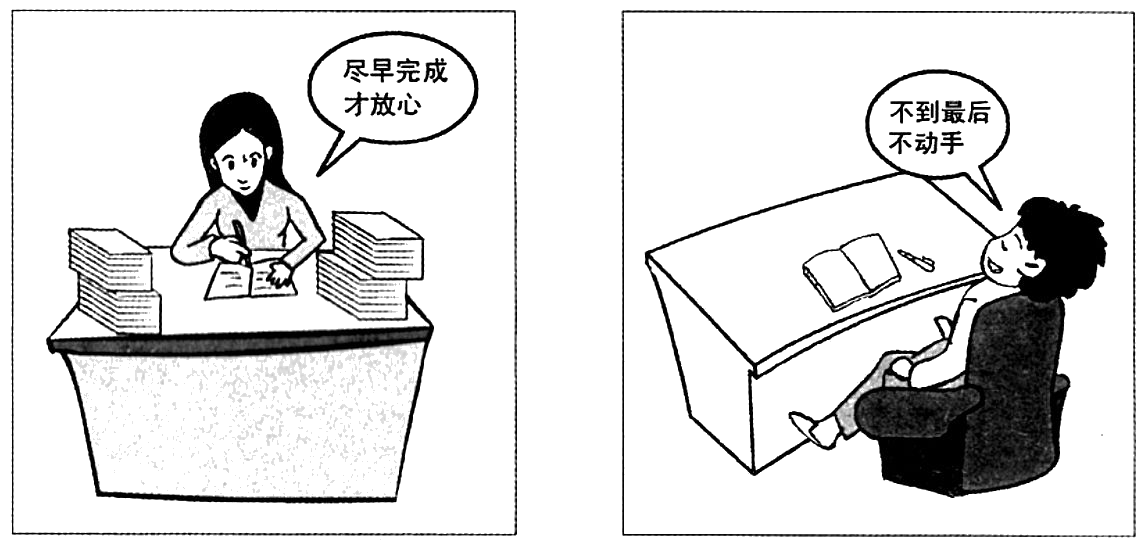
\includegraphics[width=0.76\linewidth]{picture/2020.png}
	\caption*{习惯}
\end{figure}




%

\bta{2021}


\section{Use of English}

\noindent
\textbf{Directions:}\\
Read the following text. Choose the best word (s) for each numbered
	blank and mark A, B, C or D on the ANSWER SHEET.
	(10 points)


\TiGanSpace



	Fluid intelligence is the type of intelligence that has to do with
	short-term memory and the ability to think quickly, logically, and
	abstractly in order to solve new problems. It \cloze in young
	adulthood, levels out for a period of time, and then \cloze starts to
	slowly decline as we age. But \cloze aging is inevitable, scientists
	are finding that certain changes in brain function may not be.
	
	One study found that muscle loss and the \cloze of body fat around the
	abdomen are associated with a decline in fluid intelligence. This
	suggests the \cloze that lifestyle factors might help prevent or
	\cloze this type of decline.
	
	The researchers looked at data that \cloze measurements of lean
	muscle and abdominal
	fat from more than 4, 000 middle-to-older-aged men and women and
	\cloze that data to reported changes in fluid intelligence over a
	six-year period. They found that middle-aged people
	\cloze higher measures of abdominal fat \cloze worse on
	measures of fluid intelligence as the years \cloze.
	
	For women, the association may be \cloze to changes in immunity
	that resulted from excess abdominal fat; in men, the immune system did
	not appear to be \cloze. It is hoped that future studies could
	\cloze these differences and perhaps lead to different
	\cloze for men and women.
	
	\cloze , there are steps you can \cloze to help reduce
	abdominal fat and maintain lean muscle mass as you age in order to
	protect both your physical and mental \cloze. The two highly
	recommended lifestyle approaches are maintaining or increasing your
	\cloze of aerobic exercise and following a Mediterranean-style
	\cloze that is high in fiber and eliminates highly processed
	foods.


\newpage

\begin{enumerate}
	%\renewcommand{\labelenumi}{\arabic{enumi}.}
	% A(\Alph) a(\alph) I(\Roman) i(\roman) 1(\arabic)
	%设定全局标号series=example	%引用全局变量resume=example
	%[topsep=-0.3em,parsep=-0.3em,itemsep=-0.3em,partopsep=-0.3em]
	%可使用leftmargin调整列表环境左边的空白长度 [leftmargin=0em]
	\item
\fourchoices
{pauses}
{returns}
{peaks}
{fades}

	

\item 			
\fourchoices
{alternatively}
{formally}
{accidentally}
{generally}


			
\item
			
\fourchoices
{while}
{since}
{once}
{until}

	
\item 
\fourchoices
{detection}
{accumulation}
{consumption}
{separation}


\item
			
\fourchoices
{possibility}
{decision}
{goal}
{requirement}

	
\item 
\fourchoices
{delay}
{ensure}
{seek}
{utilize}

	
\item 
\fourchoices
{modified}
{supported}
{included}
{predicted}

	
\item 
\fourchoices
{devoted}
{compared}
{converted}
{applied}

	
\item 
\fourchoices
{with}
{above}
{by}
{against}

	
\item 
\fourchoices
{lived}
{managed}
{scored}
{played}

	
\item 
\fourchoices
{ran out}
{set off}
{drew in}
{went by}

	
\item 
\fourchoices
{superior}
{attributable}
{parallel}
{resistant}

	
\item 
\fourchoices
{restored}
{isolated}
{involved}
{controlled}

	
\item 
\fourchoices
{alter}
{spread}
{remove}
{explain}

	
\item 
\fourchoices
{compensations}
{symptoms}
{demands}
{treatments}

	
\item 
\fourchoices
{Likewise}
{Meanwhile}
{Therefore}
{Instead}

	
\item 
\fourchoices
{change}
{watch}
{count}
{take}

	
\item 
\fourchoices
{well-being}
{process}
{formation}
{coordination}

	
\item 
\fourchoices
{level}
{love}
{knowledge}
{space}

\item 
\fourchoices
{design}
{routine}
{diet}
{prescription}


\end{enumerate}


\vfil

\section{Reading Comprehension}



\noindent
\textbf{Part A}\\
\textbf{Directions:}\\
Read the following four texts. Answer the questions after each
text by choosing A, B, C or
D. Mark your answers
on the ANSWER SHEET. (40 points)


\newpage
\subsection{Text 1}



How can the train operators possibly justify yet another increase to
rail passenger fares? It has become a grimly reliable annual ritual:
every January the cost of travelling by train rises, imposing a
significant extra burden on those who have no option but to use the rail
network to get to work or otherwise. This year's rise, an average of 2.7
percent, may be a fraction lower than last year's, but it is still well
above the official Consumer Price Index (CPI) measure of inflation.

Successive governments have permitted such increases on the grounds that
the cost of investing in and running the rail network should be borne by
those who use it, rather than the general taxpayer. Why, the argument
goes, should a car-driving pensioner from Lincolnshire have to subsidise
the daily commute of a stockbroker from Surrey? Equally, there is a
sense that the travails of commuters in the South East, many of whom
will face among the biggest rises, have received too much attention
compared to those who must endure the relatively poor infrastructure of
the Midlands and the North.

However, over the past 12 months, those commuters have also experienced
some of the worst rail strikes in years. It is all very well train
operators trumpeting the improvements they are making to the network,
but passengers should be able to expect a basic level of service for the
substantial sums they are now paying to travel. The responsibility for
the latest wave of strikes rests on the unions. However, there is a
strong case that those who have been worst affected by industrial action
should receive compensation for the disruption they have suffered.

The Government has pledged to change the law to introduce a minimum
service requirement so that, even when strikes occur, services can
continue to operate. This should form part of a wider package of
measures to address the long-running problems on Britain's railways.
Yes, more investment is needed, but passengers will not be willing to
pay more indefinitely if they must also endure cramped, unreliable
services, punctuated by regular chaos when timetables are changed, or
planned maintenance is managed incompetently. The threat of
nationalisation may have been seen off for now, but it will return with
a vengeance if the justified anger of passengers is not addressed in
short order.

\vspace{1em}

\begin{enumerate}[resume]
	%\renewcommand{\labelenumi}{\arabic{enumi}.}
	% A(\Alph) a(\alph) I(\Roman) i(\roman) 1(\arabic)
	%设定全局标号series=example	%引用全局变量resume=example
	%[topsep=-0.3em,parsep=-0.3em,itemsep=-0.3em,partopsep=-0.3em]
	%可使用leftmargin调整列表环境左边的空白长度 [leftmargin=0em]
	\item
The author holds that this year's increase in rail passengers fares \lineread.


\fourchoices
{will ease train operation's burden}
{has kept pace with inflation}
{is a big surprise to commuters}
{remains an unreasonable measure}


\item
The stockbroker in Para. 2 is used to stand for \lineread.


\fourchoices
{car drivers}
{rail travellers}
{local investors}
{ordinary tax payers}


\item
 It is indicated in Para. 3 that train operators \lineread.


\fourchoices
{are offering compensations to commuters}
{are trying to repair ralations with the unions}
{have failed to provide an adequate source}
{have suffered huge losses owing to the strikes}


\item
If unable to calm down passengers, the railways may have to face \lineread.


\fourchoices
{the loss of investment}
{the collapse of operations}
{a reduction of revenue}
{a change of ownership}



\item
 Which of the following would be the best title for the text?


\fourchoices
{Who Are to Blame for the Strikes?}
{Constant Complaining Doesn't Worlk}
{Can Nationalization Bring Hope?}
{Ever-rising Fares Aren't Sustainable	}

	
\end{enumerate}





\newpage
\subsection{Text 2}



Last year marked the third year in a row of when Indonesia's bleak rate
of deforestation has slowed in pace. One reason for the turnaround may
be the country's antipoverty program.

In 2007, Indonesia started phasing in a program that gives money to its
poorest residents under certain conditions, such as requiring people to
keep kids in school or get regular medical care. Called conditional cash
transfers or CCTs, these social assistance programs are designed to
reduce inequality and break the cycle of poverty. They're already used
in dozens of countries worldwide. In Indonesia, the program has provided
enough food and medicine to substantially reduce severe growth problems
among children.

But CCT programs don't generally consider effects on the environment. In
fact, poverty alleviation and environmental protection are often viewed
as conflicting goals, says Paul Ferraro, an economist at Johns Hopkins
University.

That's because economic growth can be correlated with environmental
degradation, while protecting the environment is sometimes correlated
with greater poverty. However, those correlations don't prove cause and
effect. The only previous study analyzing causality, based on an area in
Mexico that had instituted CCTs, supported the traditional view. There,
as people got more money, some of them may have more cleared land for
cattle to raise for meat, Ferraro says.

Such programs do not have to negatively affect the environment, though.
Ferraro wanted to see if Indonesia's poverty-alleviation program was
affecting deforestation. Indonesia has the third-largest area of
tropical forest in the world and one of the highest deforestation rates.

Ferraro analyzed satellite data showing annual forest loss from 2008 to
2012---including during Indonesia's phase-in of the antipoverty
program---in 7, 468 forested villages across 15 provinces . 
 ``we see that the program is
associated with a 30 percent reduction in deforestation,'' Ferraro says.

That's likely because the rural poor are using the money as makeshift
insurance policies against inclement weather, Ferraro says. Typically,
if rains are delayed, people may clear land to plant more rice to
supplement their harvests. With the CCTs, individuals instead can use
the money to supplement their harvests.

Whether this research translates elsewhere is anybody's guess. Ferraro
suggests
the results may transfer to other parts of Asia, due to
commonalities such as the
 the importance of growing rice and market access. And
regardless of transferability, the study shows that what's good for
people may also be good for 
 the environment. Even if this program didn't
reduce poverty, Ferraro says, ``the value of the avoided deforestation just for
carbon dioxide emissions alone is more than the program costs.''


\begin{enumerate}[resume]
	%\renewcommand{\labelenumi}{\arabic{enumi}.}
	% A(\Alph) a(\alph) I(\Roman) i(\roman) 1(\arabic)
	%设定全局标号series=example	%引用全局变量resume=example
	%[topsep=-0.3em,parsep=-0.3em,itemsep=-0.3em,partopsep=-0.3em]
	%可使用leftmargin调整列表环境左边的空白长度 [leftmargin=0em]
	\item
According to the first two paragraphs, CCT programs aim to \lineread.


\fourchoices
{facilitate health care reform}
{help poor families get better off}
{improve local education systems}
{lower deforestation rates}


\item
 The study based on an area in Mexico is cited to show that \lineread.


\fourchoices
{cattle rearing has been a major means of livelihood for the poor}
{CCT programs have helped preserve traditional lifestyles}
{antipoverty efforts require the participation of local farmers}
{economic growth tends to cause environmental degradation}



\item
 In his study about Indonesia, Ferraro intends to find out \lineread.


\fourchoices
{its acceptance level of CCTs}
{its annual rate of poverty alleviation}
{the relation of CCTs to its forest loss}
{the role of its forests in climate change}



\item
According to Ferraro, the CCT program in Indonesia is most valuable
in that \lineread.


\fourchoices
{it will benefit other Asian countries}
{it will reduce regional inequality}
{it can protect the environment}
{it can boost grain production}


\item
What is the text centered on?


\fourchoices
{The effects of a program.}
{The debates over a program.}
{The process of a study.}
{The transferability of a study.	}

	
\end{enumerate}




\newpage
\subsection{Text 3}



As a historian, who's always searching for the text or the image that
makes us re-evaluate the past. I've become preoccupied with looking for
photographs that show our Victorian ancestors smiling (what better way
to shatter the image of 19th-century prudery?). I've found quite a few,
and---since I started posting them on Twitter---they have been causing
quite a stir. People have been surprised to see evidence that Victorians
had fun and could, and did, laugh. They are noting that the Victorians
suddenly seem to become more human as the hundred-or-so years that
separate us fade away through our common experience of laughter.

Of course, I need to concede that my collection of ``Smiling
Victorians'' makes up only a tiny percentage of the vast catalogue of
photographic portraiture created between 1840 and 1900, the majority of
which show sitters posing miserably and stiffly in front of painted
backdrops, or staring absently into the middle distance. How do we
explain this trend?

During the 1840s and 1850s, in the early days of photography, exposure
times were notoriously long: the daguerreotype photographic method
(producing an image on a silvered copper plate) could take several
minutes to complete, resulting in blurred images as sitters shifted
position or adjusted their limbs. The thought of holding a fixed grin as
the camera performed its magical duties was too much to contemplate, and
so a non-committal blank stare became the norm.

But exposure times were much quicker by the 1880 s, and the introduction
of the Box Brownie and other portable cameras meant that, though slow by
today's digital standards, the exposure was almost instantaneous.
Spontaneous smiles were relatively easy to capture by the 1890 s, so we
must look elsewhere for an explanation of why Victorians still hesitated
to smile.

One explanation might be the loss of dignity displayed through a cheesy
grin. ``Nature gave us lips to conceal our teeth,'' ran one popular
Victorian maxim, alluding to the fact that before the birth of proper
dentistry, mouths were often in a shocking state of hygiene. A flashing
set of healthy and clean, regular ``pearly whites'' was a rare sight in
Victorian society, the preserve of the super-rich (and even then, dental
hygiene was not guaranteed).

A toothy grin (especially when there were gaps or blackened gnashers)
lacked class: drunks, tramps, prostitutes and buffoonish music hall
performers might gurn and grin with a smile as wide as Lewis Carroll's
gum-exposing Cheshire Cat, but it was not a becoming look for properly
bred persons. Even Mark Twain, a man who enjoyed a hearty laugh, said
that when it came to photographic portraits there could be ``nothing
more damning than a silly, foolish smile fixed forever''.


\begin{enumerate}[resume]
	%\renewcommand{\labelenumi}{\arabic{enumi}.}
	% A(\Alph) a(\alph) I(\Roman) i(\roman) 1(\arabic)
	%设定全局标号series=example	%引用全局变量resume=example
	%[topsep=-0.3em,parsep=-0.3em,itemsep=-0.3em,partopsep=-0.3em]
	%可使用leftmargin调整列表环境左边的空白长度 [leftmargin=0em]
	\item
According to Paragraph 1, the author's posts on Twitter \lineread.


\fourchoices
{illustrated the development of Victorian photography}
{highlighted social media's role in Victorian studies}
{re-evaluated the Victorian's notion of public image}
{changed people's impression of the Victorians}


\item
What does the author say about the Victorian portraits he has
collected?


\fourchoices
{They are rare among photographs of that age.}
{They show effects of different exposure times.}
{They mirror 19th-century social conventions.}
{They are in popular use among historians.}



\item
 What might have kept the Victorians from smiling for pictures in the
1890s?


\fourchoices
{Their inherent social sensitiveness.}
{Their tension before the camera.}
{Their distrust of new inventions.}
{Their unhealthy dental condition.}



\item
Mark Twain is quoted to show that the disapproval of smiles in
pictures was \lineread.


\fourchoices
{a deep-root belief}
{a misguided attitude}
{a controversial view}
{a thought-provoking idea}


\item
Which of the following questions does the text answer?


\fourchoices
{Why did most Victorians look stern in photographs?}
{Why did the Victorians start to view photographs?}
{What made photography develop slowly in the Victorian period?}
{How did smiling in photographs become a post-Victorian norm?	}
	
	
\end{enumerate}



\newpage
\subsection{Text 4}



From the early days of broadband, advocates for consumers and web-based
companies worried that the cable and phone companies selling broadband
connections had the power and incentive to favor their own or their
partners' websites and services over those of their rivals. That's why
there has been such a strong demand for rules that would prevent
broadband providers from picking winners and losers online, preserving
the freedom and innovation that have been the lifeblood of the internet.

Yet that demand has been almost impossible to fill---in part because
of pushback from broadband providers, anti-regulatory conservatives and
the courts. A federal appeals court weighed in again Tuesday, but
instead of providing a badly needed resolution, it only prolonged the
fight. At issue before the U.S. Court of Appeals for the District of
Columbia Circuit was the latest take of the Federal Communications
Commission (FCC) on net neutrality, adopted on a party-line vote in 2017. The
Republican penned order not only eliminated the strict net neutrality
rules the FCC had adopted when it had a Democratic majority in 2015, but
rejected the commission's authority to require broadband providers to do
much of anything. The order also declared that state and local
governments couldn't regulate broadband providers either.

The commission argued that other agencies would protect against
anti-competitive behavior, such as a broadband-providing conglomerate
like AT\&T favoring its own video-streaming service at the expense of
Netflix and Apple TV. Yet the FCC also ended the investigations of
broadband providers that imposed data caps on their rivals' streaming
services but not their own.

On Tuesday, the appeals court unanimously upheld the 2017 order
deregulating broadband providers, citing a Supreme Court ruling from
2005 that upheld a similarly deregulatory move. But Judge Patricia
Millett rightly argued in a concurring opinion that ``the result is
unhinged from the realities of modern broadband service,'' and said
Congress or the Supreme Court could intervene to ``avoid trapping
Internet regulation in technological anachronism.''

In the meantime, the court threw out the FCC's attempt to block all
state rules on net neutrality, while preserving the commission's power
to pre-empt individual state laws that undermine its order. That means
more battles like the one now going on between the Justice Department
and California, which enacted a tough net neutrality law in the wake of
the FCC's abdication.

The endless legal battles and back-and-forth at the FCC cry out for
Congress to act. It needs to give the commission explicit authority once
and for all to bar broadband providers from meddling in the traffic on
their network and to create clear rules protecting openness and
innovation online.

\begin{enumerate}[resume]
	%\renewcommand{\labelenumi}{\arabic{enumi}.}
	% A(\Alph) a(\alph) I(\Roman) i(\roman) 1(\arabic)
	%设定全局标号series=example	%引用全局变量resume=example
	%[topsep=-0.3em,parsep=-0.3em,itemsep=-0.3em,partopsep=-0.3em]
	%可使用leftmargin调整列表环境左边的空白长度 [leftmargin=0em]
	\item
There has long been concern that broadband provides would \lineread.


\fourchoices
{bring web-based firms under control}
{slow down the traffic on their network}
{show partiality in treating clients}
{intensify competition with their rivals}


\item
Faced with the demand for net neutrality rules, the FCC \lineread.


\fourchoices
{sticks to an out-of-date order}
{takes an anti-regulatory stance}
{has issued a special resolution}
{has allowed the states to intervene}



\item
What can be learned about AT\&T from Paragraph 3?


\fourchoices
{It protects against unfair competition}
{It engages in anti-competitive practices.}
{It is under the FCC'S investigation.}
{It is in pursuit of quality service.}


\item
Judge Patricia Millett argues that the appeals court's decision \lineread.


\fourchoices
{focuses on trivialities}
{conveys an ambiguous message}
{is at odds with its earlier rulings}
{is out of touch with reality}


\item
What does the author argue in the last paragraph?


\fourchoices
{Congress needs to take action to ensure net neutrality.}
{The FCC should be put under strict supervision.}
{Rules need to be set to diversify online services.}
{Broadband providers' rights should be protected.}
	
	
	
\end{enumerate}



\newpage

\noindent
\textbf{Part B}\\
\textbf{Directions:}\\
In the following text, some sentences have been removed. For
questions 41--45, choose the most suitable one from the list A--G to fit
into each of numbered blanks. There are two extra choices, which do not
fit in any of the blanks. Mark your answers on the ANSWER SHEET. (10
points)


\TiGanSpace

In the movies and on television, artificial intelligence (AI) is
typically depicted as something sinister that will upend our way of
life. When it comes to AI in business, we often hear about it in
relation to automation and the impending loss of jobs, but in what ways
is AI changing companies and the larger economy that don't involve
doom-and-gloom mass unemployment predictions?

A recent survey of manufacturing and service industries from Tata
Consultancy Services found that companies currently use AI more often in
computer-to-computer activities than in automating human activities. 
Here are a few other ways AI is aiding companies without replacing
employees:



\textbf{Better hiring practices}


Companies are using artificial intelligence to remove some of the
unconscious bias from hiring decisions. ``There are experiments that
show that, naturally, the results of interviews are
much more biased than what AI does,'' 
says Pedro Domingos, author of \emph{The Master Algorithm: How the
	Qust for the Ultimate Learning Machine Will Remake Our World} and a
computer science professor at the University of Washington. In addition,
``  \linefill. '' One company that's doing this
is called Blendoor. It uses analytics to help identify where there may be bias
in the hiring process.



\textbf{More effective marketing}


Some AI software can analyze and optimize marketing email subject lines
to increase open rates. One company in the UK, Phrasee, claims their
software can outperform humans by up to 10 percent when it comes to
email open rates. This can mean millions more in revenue. 
\linefill.
These are ``tools that help people use data, not a replacement for
people,'' says Patrick
H. Winston, a professor of artificial
intelligence and computer science at MIT.



\textbf{Saving customers money}


Energy companies can use AI to help customers reduce their electricity
bills, saving them money while helping the environment. Companies can
also optimize their own energy use and cut down on the cost of
electricity. Insurance companies, meanwhile, can base their premiums on
AI models that more accurately access risk. Domingos says,  `` \linefill. ''




\textbf{Improved accuracy}


``Machine learning often provides a more reliable form of statistics,
which makes data more valuable,'' says Winston. It ``helps people make
smarter decisions.'' \\
\linefill.


\textbf{Protecting and Maintaining  infrastructure}


A number of companies, particularly in energy and transportation, use AI
image processing technology to inspect infrastructure and prevent
equipment failure or leaks before they happen. ``If they fail first and
then you fix them, it's very expensive,'' says Domingos. `` \linefill. ''



\begin{listmatch}
	%\renewcommand{\labelenumi}{\arabic{enumi}.}
	% A(\Alph) a(\alph) I(\Roman) i(\roman) 1(\arabic)
	%设定全局标号series=example	%引用全局变量resume=example
	%[topsep=-0.3em,parsep=-0.3em,itemsep=-0.3em,partopsep=-0.3em]
	%可使用leftmargin调整列表环境左边的空白长度 [leftmargin=0em]
	\item
I replace the boring parts of your job. If you're doing research, you
can have AI go out and look for relevant sources and information that
otherwise you just wouldn't have time for.

\item
There are also companies like Acquisio, which analyzes advertising
performance across multiple channels like Adwords, Bing and social
media and makes adjustments or suggestions about where advertising
funds will yield best results.


\item
One accounting firm, EY, uses an AI system that helps review contracts
during an audit. This process, along with employees reviewing the
contracts, is faster and more accurate.



\item
You want to predict if something needs attention now and point to
where it's useful for employees to go to.

\item
We're also giving our customers better channels versus picking up the
phone  to accomplish something beyond human scale.

\item
Before, they might not insure the ones who felt like a high risk or
charge them too much, or they would charge them too little and then it
would cost the company money.



\item
AI looks at résumés in greater numbers than humans would be able to,
and selects the more promising candidates.

\end{listmatch}


\newpage
\noindent
\textbf{Part C}\\
\textbf{Directions:}\\
Read the following text carefully and then translate the
underlined segments into Chinese. 
Write your answers on the ANSWER SHEET. (10 points)

\TiGanSpace

World War II was the watershed event for higher education in modern
western societies. \transnum \uline{Those societies came out of the war
with levels of enrollment that had been roughly constant at 3-5\% of the relevant age groups during the decades before
the war}. But after the war, great social and political changes arising
out of the successful war against Fascism created a growing demand in
European and American economies for increasing numbers of graduates with
more than a
secondary school education. \transnum \uline{And the demand that rose in
those societies for entry to higher education extended to groups and social classes that had not
thought of attending to a university before the war}. These demands resulted in a very rapid
expansion of the systems of higher education, beginning in the 1960s and
developing very rapidly (though unevenly) during the 1970s and 1980s.



The growth of higher education manifests itself in at least three quite
different ways, and these in turn have given rise to different sets of
problems. There was first  \emph{the rate of growth}: \transnum \uline{in many
countries of Western Europe the numbers of students in higher education
doubled within five-year periods during the decade of the 1960s and doubled
again in seven, eight, or 10 years by the middle of the 1970 s}. Second, growth obviously affected
the \emph{absolute size} both of systems and individual institutions.
And third, growth was reflected in changes in \emph{the proportion of
the relevant age group} enrolled in institutions of higher education.

Each of these manifestations of growth carried its own peculiar
problems in its wake. For example, a high growth rate placed great strains
on the existing structures of governance, of administration, and above all of
socialization. When a faculty or department grows from, say, five to 20
members within three or four years, \transnum \uline{and when the new staff are
predominantly young men and women fresh from postgraduate study, they
largely define the norms of academic life in that faculty.} And if the
postgraduate student population also grows rapidly and there is loss of a
close apprenticeship relationship between faculty members and students,
the student culture becomes the chief socializing force for new postgraduate
students, with consequences for the intellectual and academic life of the
institution---this was seen in America as well as in France, Italy, West
Germany, and Japan. \transnum  \uline{High growth rates increased the chances for
academic innovation; they also weakened the forms and processes by which
teachers and students are admitted into a community of scholars during
periods of stability or slow growth.} In the 1960s and 1970s, European
universities saw marked changes in their governance arrangements, with the
empowerment of junior faculty and to some degree of students as well.



\newpage

\section{Writing}



\noindent
\textbf{Part A}\\
\textbf{51. Directions:}


A foreign friend of yours has recently graduated from college and
intends to find a job in China. Write him/her an email to make some
suggestions.


You should write about 100 words on the ANSWER SHEET.



\textbf{Do not} use your own name in the email. Use `` Li Ming''
instead. (10 points)

\vspace{2em}

\noindent
\textbf{Part B}\\
\textbf{52. Directions:}



Write an essay of 160-200 words based on the pictures below. In
your essay, you should


\begin{listwrite}
	\item 
	describe the picture briefly,
	
	\item 
	interpret its intended meaning, and
	
	\item 
	give your comments.
\end{listwrite}

You should write neatly on the ANSWER SHEET. (20 points)


\begin{figure}[h!]
	\centering
	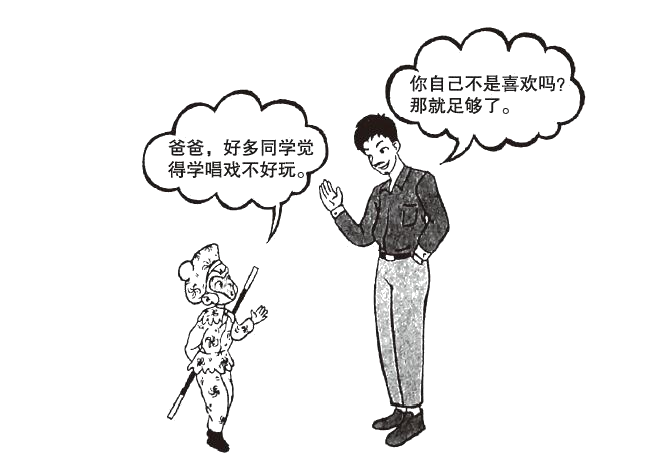
\includegraphics[width=0.64\linewidth]{picture/2021.png}
\end{figure}




\checkpagenumber%
\bta{2022}


\section{Use of English}

\noindent
\textbf{Directions:}\\
Read the following text. Choose the best word(s) for each numbered blank
and mark A, B, C or D on the
ANSWER SHEET. (10 points)

\TiGanSpace


The idea that plants have some degree of consciousness first took root
in the early 2000s; the term ``plant
neurobiology'' was  \cloze around the notion that some aspects of plant behavior could be
\cloze 
to intelligence in
animals.
 \cloze 
plants lack brains, the firing of electrical signals in their stems and
leaves nonetheless triggered
responses that  \cloze 
consciousness, researchers previously reported.


But such an idea is untrue, according to a new opinion article. Plant
biology is complex and fascinating, but it
 \cloze 
so greatly from that of animals that so-called
 \cloze 
 of plants' intelligence is inconclusive, the authors wrote.
 
 
Beginning in 2006, some scientists have
 \cloze 
 that plants possess neuron-like cells that interact with
hormones and neurotransmitters,
 \cloze 
``a plant nervous system,  \cloze 
to that in animals,'' said lead study author 
Lincoln Taiz, ``They  \cloze claimed that plants have `brain-like command centers' at their root
tips.''



This
 \cloze 
makes sense if you simplify the workings of a complex brain,
 \cloze 
it to an array of electrical pulses; cells in plants also communicate through electrical signals.
 \cloze , the signaling in a plant is only
 \cloze 
similar to the firing in a complex animal brain, which is more than ``a
mass of cells that communicate by
electricity,'' Taiz said.



``For consciousness to evolve, a brain with a threshold
 \cloze 
of complexity and capacity is required,'' he 
  \cloze . ``Since plants don't have nervous systems, the
 \cloze 
that they have consciousness are effectively zero.''


And what's so great about consciousness, anyway? Plants can't run away
from
 \cloze , so investing energy in
a body system which
 \cloze 
a threat and can feel pain would be a very
 \cloze 
evolutionary strategy, according to
the article.

\newpage

\begin{enumerate}
	%\renewcommand{\labelenumi}{\arabic{enumi}.}
	% A(\Alph) a(\alph) I(\Roman) i(\roman) 1(\arabic)
	%设定全局标号series=example	%引用全局变量resume=example
	%[topsep=-0.3em,parsep=-0.3em,itemsep=-0.3em,partopsep=-0.3em]
	%可使用leftmargin调整列表环境左边的空白长度 [leftmargin=0em]
	\item

\fourchoices
{coined}
{discovered}
{collected}
{issued}



\item

\fourchoices
{attributed}
{directed}
{compared}
{confined}

\item

\fourchoices
{Unless}
{When}
{Once}
{Though}


\item

\fourchoices
{cope with}
{consisted of}
{hinted at}
{extended in}


\item

\fourchoices
{suffers}
{benefits}
{develops}
{differs}


\item

\fourchoices
{acceptance}
{evidence}
{cultivation}
{creation}


\item
\fourchoices
{doubted}
{denied}
{argued}
{requested}


\item

\fourchoices
{adapting}
{forming}
{repairing}
{testing}

\item 
\fourchoices
{analogous}
{essential}
{suitable}
{sensitive}


\item

\fourchoices
{just}
{ever}
{still}
{even}



\item

\fourchoices
{restriction}
{experiment}
{perspective}
{demand}


\item

\fourchoices
{attaching}
{reducing}
{returning}
{exposing}



\item

\fourchoices
{However}
{Moreover}
{Therefore}
{Otherwise}


\item
\fourchoices
{temporarily}
{literally}
{superficially}
{imaginarily}


\item

\fourchoices
{list}
{level}
{label}
{local}


\item

\fourchoices
{recalled}
{agreed}
{questioned}
{added}


\item

\fourchoices
{chances}
{risks}
{excuses}
{assumptions}


\item

\fourchoices
{danger}
{failure}
{warning}
{control}



\item

\fourchoices
{represents}
{includes}
{reveals}
{recognizes}


\item

\fourchoices
{humble}
{poor}
{practical}
{easy}


\end{enumerate}


\vfil

\section{Reading Comprehension}


\noindent
\textbf{Part A}\\
\textbf{Directions:}\\
Read the following four texts. Answer the questions below each text by
choosing A, B, C or
D. Mark your
answers on the ANSWER SHEET. (40 points)





\newpage

\subsection{Text 1}

People often complain that plastics are too durable. Water
bottles, shopping bags, and other trash litter the
planet, from Mount Everest to the Mariana Trench, because plastics are
everywhere and don't break down easily.
But some plastic materials change over time. They crack and frizzle.
They ``weep'' out additives. They melt into
sludge. All of which creates huge headaches for institutions, such as
museums, trying to preserve culturally
important objects. The variety of plastic objects at risk is dizzying:
early radios, avant-garde sculptures, celluloid
animation stills from Disney films, the first artificial heart.


Certain artifacts are especially vulnerable because some pioneers in
plastic art didn't always know how to
mix ingredients properly, says Thea van Oosten, a polymer chemist who,
until retiring a few years ago, worked for
decades at the Cultural Heritage Agency of the Netherlands. ``It s like
baking a cake: If you don't have exact
amounts, it goes wrong.'' she says. ``The object you make is already a
time bomb.''



And sometimes, it's not the artist's fault. In the 1960 s, the Italian
artist Picro Gilardi began to create hundreds
of bright, colorful foam pieces. Those pieces included small beds of
roses and other items as well as a few dozen
``nature carpets''---large rectangles decorated with foam pumpkins,
cabbages, and watermelons. He wanted
viewers to walk around on the carpets---which meant they had to be
durable.



Unfortunately, the polyurethane foam he used is inherently unstable.
It's especially vulnerable to light
damage, and by the mid-1990s, Gilardi's pumpkins, roses, and other
figures were splitting and crumbling.
Museums locked some of them away in the dark.




So van Oosten and her colleagues worked to preserve Gilardi's
sculptures. They infused some with stabilizing
and consolidating chemicals. Van Oosten calls those chemicals
``sunscreens'' because their goal was to prevent
further light damage and rebuild worn polymer fibers. She is proud that
several sculptures have even gone on
display again, albeit sometimes beneath protective cases.




Despite success stories like van Oosten's, preservation of plastics will
likely get harder. Old objects continue
to deteriorate. Worse, biodegradable plastics designed to disintegrate,
are increasingly common.



And more is at stake here than individual objects. Joana Lia Ferreira, an
assistant professor of conservation
and restoration at the nova School of Science and Technology, notes that
archaeologists first defined the great
material ages of human history Stone Age, Iron Age, and so on after
examining artifacts in museums. We now live
in an age of plastic, she says, ``and what we decide to collect
today, what we decide to preserve\ldots will have a
strong impact on how in the future we'll be seen.''


\begin{enumerate}[resume]
	%\renewcommand{\labelenumi}{\arabic{enumi}.}
	% A(\Alph) a(\alph) I(\Roman) i(\roman) 1(\arabic)
	%设定全局标号series=example	%引用全局变量resume=example
	%[topsep=-0.3em,parsep=-0.3em,itemsep=-0.3em,partopsep=-0.3em]
	%可使用leftmargin调整列表环境左边的空白长度 [leftmargin=0em]
	\item
According to Paragraph 1, museums are faced with difficulties
in \lineread.


\fourchoices
{maintaining their plastic items}
{obtaining durable plastic artifacts}
{handling outdated plastic exhibits}
{classifying their plastic collections}



\item
Van Oosten believes that certain plastic objects are \lineread.


\fourchoices
{immune to decay}
{improperly shaped}
{inherently flawed}
{complex in structure}



\item
 Museums stopped exhibiting some of Gilardi's artworks to
\lineread.


\fourchoices
{keep them from hurting visitors}
{duplicate them for future display}
{have their ingredients analyzed}
{prevent them from further damage}



\item
The author thinks that preservation of plastics is \lineread.


\fourchoices
{costly}
{unworthy}
{unpopular}
{challenging}



\item
In Ferreira's opinion, preservation of plastic artifacts
\lineread.


\fourchoices
{will inspire future scientific research}
{has profound historical significance}
{will help us separate the material ages}
{has an impact on today's cultural life}

\end{enumerate}


\newpage
\subsection{Text 2}

As the latest crop of students pen their undergraduate application form
and weigh up their options, it may be
worth considering just how the point, purpose and value of a degree has
changed and what Generation Z need to
consider as they start the third stage of their educational journey.



Millennials were told that if you did well in school, got a decent
degree, you would be set up for life. But that
promise has been found wanting. As degrees became universal, they became
devalued. Education was no longer a
secure route of social mobility. Today, 28 per cent of graduates in the
UK are in non-graduate roles, a percentage
which is double the average among OECD countries.



This is not to say that there is no point in getting a degree, but
rather stress that a degree is not for everyone,
that the switch from classroom to lecture hall is not an inevitable one
and that other options are available.




Thankfully, there are signs that this is already happening, with
Generation Z seeking to learn from their
millennial predecessors, even if parents and teachers tend to be still
set in the degree mindset. Employers have
long seen the advantages of hiring school leavers who often prove
themselves to be more committed and loyal
employees than graduates. Many too are seeing the advantages of
scrapping a degree requirement for certain roles.




For those for whom a degree is the desired route, consider that this may
well be the first of many. In this age
of generalists, it pays to have specific knowledge or skills.
Postgraduates now earn 40 per cent more than
graduates. When more and more of us have a degree, it makes sense to
have two.




It is unlikely that Generation Z will be done with education at 18 or
21; they will need to be constantly
up-skilling throughout their career to stay employable. It has been
estimated that this generation, due to the
pressures of technology, the wish for personal fulfilment and desire for
diversity, will work for 17 different
employers over the course of their working life and have five different
careers. Education, and not just knowledge
gained on campus, will be a core part of Generation Z's career
trajectory.



Older generations often talk about their degree in the present and
personal tense: `I am a geographer.' or `I
am a classist.' Their sons or daughters would never say such a thing;
it's as if they already know that their degree
won't define them in the same way.

\begin{enumerate}[resume]
	%\renewcommand{\labelenumi}{\arabic{enumi}.}
	% A(\Alph) a(\alph) I(\Roman) i(\roman) 1(\arabic)
	%设定全局标号series=example	%引用全局变量resume=example
	%[topsep=-0.3em,parsep=-0.3em,itemsep=-0.3em,partopsep=-0.3em]
	%可使用leftmargin调整列表环境左边的空白长度 [leftmargin=0em]
	\item
 The author suggests that Generation Z should \lineread.


\fourchoices
{be careful in choosing a college}
{be diligent at each educational stage}
{reassess the necessity of college education}
{postpone their undergraduate application}


\item
The percentage of UK graduates in non-graduate roles
reflect \lineread.


\fourchoices
{Millennial's opinions about work}
{the shrinking value of a degree}
{public discontent with education}
{the desired route of social mobility}



\item
 The author considers it a good sign that \lineread.


\fourchoices
{Generation Z are seeking to earn a decent degree}
{School leavers are willing to be skilled workers}
{Employers are taking a realistic attitude to degrees}
{Parents are changing their minds about education}



\item
It is advised in Paragraph 5 that those with one degree
should \lineread.


\fourchoices
{make an early decision on their career}
{attend on the job training programs}
{team up with high-paid postgraduates}
{further their studies in a specific field}



\item
What can be concluded about Generation Z from the last two
paragraphs?


\fourchoices
{Lifelong learning will define them.}
{They will make qualified educators.}
{Degrees will no longer appeal them.}
{They will have a limited choice of jobs.}

\end{enumerate}


\newpage
\subsection{Text 3}


Enlightening, challenging, stimulating, fun. These were some of the words
that Nature readers used to
describe their experience of art-science collaborations in a series of
articles on partnerships between artists and
researchers. Nearly 40\% of the roughly 350 people who responded to an
accompanying poll said, they had
collaborated with artists, and almost all said they would consider doing
so in future.




Such an encouraging results is not surprising. Scientists are
increasingly seeking out visual artists to help
them communicate their work to new audiences. ``Artists help scientists
reach a broader audience and make
emotional connections that enhance learning.'' One respondent said.



One example of how artists and scientists have together rocked the
scenes came last month when the Sydney
Symphony Orchestra performed a reworked version of Antonio Vivaldi's The
Four Seasons. They reimagined the
300-year-old score by injecting the latest climate prediction data for
each season-provided by Monash University's
Climate Change Communication Research Hub. The performance was a
creative call to action ahead of
November's United Nations Climate Change Conference in Glasgow, UK.




But a genuine partnership must be a two-way street. Fewer artist than
scientists responded to the Nature poll,
however, several respondents noted that artists do not simply assist
scientists with their communication
requirements. Nor should their work be considered only as an object of
study. The alliances are most valuable
when scientists and artists have a shared stake in a project, are able
to jointly design it and can critique each
other's work. Such an approach can both prompt new research as well as
result in powerful art.




More than half a century ago, the Massachusetts Institute of Technology
opened its Center for Advanced
Visual Studies (CAVS) to explore the role of technology in culture. The
founders deliberately focused their
projects around light-hance the ``visual studies'' in the name. Light
was a something that both artists and scientists
had an interest in and therefore could form the basis of collaboration.
As science and technology progressed, and
divided into more sub-disciplines, the centre was simultaneously looking
to a time when leading researchers could
also be artists, writers and poets, and vice versa.



Nature's poll findings suggest that this trend is as strong as ever, but,
to make a collaboration work both sides
need to invest time and embrace surprise and challenge. The reach of
art-science tie-ups needs to go beyond the
necessary purpose of research communication, and participants. Artists
and scientists alike are immersed in
discovery and invention, and challenge and critique are core to
both, too.

\begin{enumerate}[resume]
	%\renewcommand{\labelenumi}{\arabic{enumi}.}
	% A(\Alph) a(\alph) I(\Roman) i(\roman) 1(\arabic)
	%设定全局标号series=example	%引用全局变量resume=example
	%[topsep=-0.3em,parsep=-0.3em,itemsep=-0.3em,partopsep=-0.3em]
	%可使用leftmargin调整列表环境左边的空白长度 [leftmargin=0em]
	\item
 According to paragraph 1, art-science collaborations have \lineread.


\fourchoices
{caught the attention of critics}
{received favorable responses}
{promoted academic publishing}
{sparked heated public disputes}



\item
The reworked version of The Four Seasons is mentioned to show
that \lineread.


\fourchoices
{art can offer audiences easy access to science}
{science can help with the expression of emotions}
{public participation in science has a promising future}
{art is effective in facilitating scientific innovations}



\item
 Some artists seem to worry about in the art-science
partnership \lineread.


\fourchoices
{their role may be underestimated}
{their reputation may be impaired}
{their creativity may be inhibited}
{their work may be misguided}



\item
 What does the author say about CAVS?

\fourchoices
{It was headed alternately by artists and scientists.}
{It exemplified valuable art-science alliances.}
{Its projects aimed at advancing visual studies.}
{Its founders sought to raise the status of artists.}


\item
In the last paragraph, the author holds that art-science
collaborations \lineread.

\fourchoices
{are likely to go beyond public expectations}
{will intensify interdisciplinary competition}
{should do more than communicating science}
{are becoming more popular than before}



\end{enumerate}


\newpage
\subsection{Text 4}


The personal grievance provisions of New Zealand's Employment Relations
Act 2000 (ERA) prevent an
employer from firing an employee without good cause. Instead, dismissals
must be justified. Employers must both
show cause and act in a procedurally fair way.



Personal grievance procedures were designed to guard the jobs of
ordinary workers from ``unjustified
dismissals'' The premise was that the common law of contract lacked
sufficient safeguards for workers against
arbitrary conduct by management. Long gone are the days when a boss
could simply give an employee contractual
notice.




But these provisions create difficulties for businesses when applied to
highly paid managers and executives.
As countless boards and business owners will attest, constraining firms
from firing poorly performing,
high-earning managers is a handbrake on boosting productivity and
overall performance. The difference between
C-grade and A-grade managers may very well be the difference between
business success or failure. Between
preserving the jobs of ordinary workers or losing them. Yet mediocrity
is no longer enough to justify a dismissal.
Consequently-and paradoxically - laws introduced to protect the jobs of
ordinary workers may be placing those
jobs at risk.




If not placing jobs at risk, to the extent employment protection laws
constrain business owners from
dismissing under-performing managers, those laws act as a constraint on
firm productivity and therefore on
workers' wages. Indeed, in ``An International Perspective on New
Zealand's Productivity Paradox'' (2014), the
Productivity Commission singled out the low quality of managerial
capabilities as a cause of the country's poor
productivity growth record.




Nor are highly paid managers themselves immune from the harm caused by
the ERA's unjustified dismissal
procedures. Because employment protection laws make it costlier to fire
an employee, employers are more
cautious about hiring new staff. This makes it harder for the marginal
manager to gain employment. And firms pay
staff less because firms carry the burden of the employment arrangement
going wrong.




Society also suffers from excessive employment protections. Stringent
job dismissal regulations adversely
affect productivity growth and hamper both prosperity and overall
well-being.




Across the Tasman Sea, Australia deals with the unjustified dismissal
paradox by excluding employees
earning above a specified ``high-income threshold'' from the protection
of its unfair dismissal laws. In New
Zealand, a 206 private members' Bill tried to permit firms and
high-income employees to contract out of the
unjustified dismissal regime. However, the mechanisms proposed were
unwieldy and the Bill was voted down
following the change in government later that year.



\begin{enumerate}[resume]
	%\renewcommand{\labelenumi}{\arabic{enumi}.}
	% A(\Alph) a(\alph) I(\Roman) i(\roman) 1(\arabic)
	%设定全局标号series=example	%引用全局变量resume=example
	%[topsep=-0.3em,parsep=-0.3em,itemsep=-0.3em,partopsep=-0.3em]
	%可使用leftmargin调整列表环境左边的空白长度 [leftmargin=0em]
	\item
 The personal grievance provisions of the ERA are intended to \lineread.


\fourchoices
{punish dubious corporate practices}
{improve traditional hiring procedures}
{exempt employers from certain duties}
{protect the rights of ordinary workers}



\item
 It can be learned from paragraph 3 that the provisions may \lineread.

\fourchoices
{hinder business development}
{undermine managers authority}
{affect the public image of the firms}
{worsen labor-management relations}


\item
 Which of the following measures would the Productivity Commission
support?


\fourchoices
{Imposing reasonable wage restraints.}
{Enforcing employment protection laws.}
{Limiting the powers of business owners.}
{Dismissing poorly performing managers.}


\item
 What might be an effect of ERA's unjustified dismissal procedures?


\fourchoices
{Highly paid managers lose their jobs.}
{Employees suffer from salary cuts.}
{Society sees a rise in overall well-being.}
{Employers need to hire new staff.}


\item
 It can be inferred that the ``high-income threshold'' in Australia \lineread.


\fourchoices
{has secured managers' earnings}
{has produced undesired results}
{is beneficial to business owners}
{is difficult to put into practice}


	
\end{enumerate}

\newpage

\noindent
\textbf{Part B}\\
\textbf{Directions:}\\
Read the following text and answer the questions by choosing the most
suitable subheading from the list
A-G for each numbered paragraphs (41-45). There are two extra subheadings
which you do not need to use.
Mark your answers on ANSWER SHEET. (10 points)

\TiGanSpace


\textbf{(41) Teri Byrd}

I was a zoo and wildlife park employee for years. Both the wildlife park
and zoo claimed to be operating for
the benefit of the animals and for conservation purposes. This claim was
false. Neither one of them actually
participated in any contributions whose bottom line is much more
important than the condition of the animals.
Animals despise being captives in zoos. No matter how you enhance
enclosures, they do not allow for freedom, a
natural diet or adequate time for transparency with these institutions,
and it's past time to eliminate zoos from our
culture.



\textbf{(42) Karen R. Sime}

As a zoology professor, I agree with Emma Marris that zoo displays can
be sad and cruel. But she
underestimates the educational value of zoos. The zoology program at my
university attracts students for whom
zoo visits were the crucial formative experience that led them to major
in biological sciences. These are mostly
students who had no opportunity as children to travel to wilderness
areas, wildlife refuges or national parks.
Although good TV shows can help stir children's interest in
conservation, they cannot replace the excitement of a
zoo visit as an intense, immersive and interactive experience. Surely
there must be some middle ground that
balances zoos treatment of animals with their educational potential.




\textbf{(43) Reg Newberry}


Emma Marris's article is an insult and a disservice to the thousands of
passionate who work tirelessly to
improve the lives of animals and protect our planet. She uses outdated
research and decades-old examples to
undermine the noble mission of organization committed to connecting
children to a world beyond their own. Zoos
are at the forefront of conservation and constantly evolving to improve
how thy care for animals and protect each
species in its natural habitat. Are there tragedies? Of course. But they
are the exception not the norm that Ms
Marris implies A distressed animal in a zoo will get as good or better
treatment than most of us at our local
hospital.




\textbf{(44) Dean Gallea}

As a fellow environmentalist animal-protection advocate and longtime
vegetarian. I could properly be in the
same camp as Emma Marris on the issue of zoos. But I believe that
well-run zoos and the heroic animals that
suffer their captivity so serve a higher purpose. Were it not for
opportunities to observe these beautiful wild
creatures close to home many more people would be driven by their
fascination to travel to wild areas to seek out
disturb and even hunt them down.
Zoos are in that sense similar to natural history and archeology museums
serving to satisfy our need for contact
with these living creatures while leaving the vast majority undisturbed
in their natural environments.



\textbf{(45) John Fraser}

Emma Marris selectively describes and misrepresents the findings of our
research. Our studies focused on
the impact of zoo experiences on how people think about themselves and
nature and the data points extracted from
our studies. Zoos are tools for thinking. Our research provides strong
support for the value of zoos in connecting
people with animals and with nature. Zoos provide a critical voice for
conservation and environmental protection.
They afford an opportunity for people from all backgrounds to encounter
a range of animals from drone bees to
springbok or salmon to better understand the natural world we live in.


\begin{listmatch}
\item 
Zoos, which spare no effort to take of animals, should not be
subjected to unfair criticism.


\item 
To pressure zoos to spend less on their animals would lead to
inhumane outcomes for the precious creatures in
their care.


\item 
 While animals in captivity deserve sympathy, zoos play a
significant role in starting young people down the
path of related sciences.


\item 
 Zoos save people trips to wilderness areas and thus contribute
to wildlife conservation.


\item 
For wild animals that cannot be returned to their natural
habitats, zoos offer the best alternative.


\item 
Zoos should have been closed down as they prioritize money
making over animals' wellbeing.


\item 
Marris distorts our findings which actually prove that zoos
serve as an indispensable link between man and
nature.


\end{listmatch}

\phantom{ \linefill \linefill \linefill \linefill \linefill}


\noindent
\textbf{Part C}\\
\textbf{Directions:}\\
Read the following text carefully and then translate the
underlined segments into Chinese. Your
translation should be written neatly on ANSWER SHEET. (10 points)

\TiGanSpace


\begin{center}
	\textbf{ 
	The Man Who Broke Napoleon's Codes-Mark Urban}
\end{center}


Between 1807 and 1814 the Iberian Peninsula (comprising Spain and
Portugal) was the scene of a titanic and
merciless struggle. It took place on many different planes: between
Napoleon's French army and the angry
inhabitants; between the British, ever keen to exacerbate the emperor's
difficulties, and the marshals sent from
Paris to try to keep them in check; between new forces of science and
meritocracy and old ones of conservatism
and birth. \transnum  \uline{It was also, and this is unknown even to many people
well read about the period, a battle between
those who made codes and those who broke them.}





I first discovered the Napoleonic cryptographic battle a few years ago
when I was reading Sir Charles
Oman's epic History of the Peninsular War. In volume V he had attached
an appendix, The Scovell Ciphers. \transnum  \uline{It
listed many documents in code that had been captured from the French
army of Spain, and whose secrets had been
revealed by the work of one George Scovell, an officer in British
headquarters.} Oman rated Scovell's significance
highly, but at the same time, the general nature of his History meant
that \transnum  \uline{he could not analyze carefully what
this obscure officer may or may not have contributed to that great
struggle between nations or indeed tell us
anything much about the man himself.} I was keen to read more, but was
surprised to find that Oman's appendix,
published in 1914, was the only considered thing that had been written
about this secret war.



I became convinced that this story was every bit as exciting and
significant as that of Enigma and the
breaking of German codes in the Second World War. The question was,
could it be told?




Studying Scovell's papers at the Public Record Office, London, I found
that he had left an extensive journal
and copious notes about his work in the Peninsula. What was more, many
original French dispatches had been
preserved in this collection, which I realized was priceless. \transnum  \uline{There
may have been many spies and intelligence
officers during the Napoleonic Wars, but it is usually extremely
difficult to find the material they actually
provided or worked on.}



Furthermore, Scovell's story involved much more than just intelligence
work. His status in Lord Wellington's
headquarters and the recognition given to him for his work were all
bound up with the class politics of the army at
the time. His tale of self-improvement and hard work would make a
fascinating biography in its own right, but
represents something more than that. \transnum  \uline{Just as the code breaking has
its wider relevance in the struggle for
Spain, so his attempts to make his way up the promotion ladder speak
volumes about British society.}




The story of Wellington himself also gripped me. Half a century ago his
campaigns were considered a central
part of the British historical mythology and spoon-fed to schoolboys.
More recently this has not been the case,
which is a great shame. A generation has grown up.



\newpage
\section{Writing}


\noindent
\textbf{Part A}\\
\textbf{51. Directions:}

Write an email to a professor at a British university, inviting him/her
to organize a team for the international
innovation contest to be held at your university.

You should write about 100 words on the ANSWER SHEET.

\textbf{Do not} use your own name in the email. Use ``Li Ming'' instead. (10
points)


\vspace{2em}

\noindent
\textbf{Part B}\\
\textbf{52. Directions:}

Write an essay of 160-200 words based on the following picture below. In
your essay, you should
\begin{listwrite}
\item 
 describe the picture briefly,

\item 
 explain its intended meaning and

\item 
 give your comments.
\end{listwrite}

You should write neatly on the ANSWER SHEET. (20 points)

\begin{figure}[h!]
	\centering
	\includesvg[width=0.55\linewidth]{picture/svg/picture-01}
\end{figure}



\checkpagenumber%
\bta{2023}


\section{Use of English}

\noindent
\textbf{Directions:}\\
Read the following text. Choose the best word(s) for each numbered blank
and mark A, B, C or D on the
ANSWER SHEET. (10 points)

\TiGanSpace

Caravanserais were roadside inns that were built along the Silk Road in areas including China, North Africa and the Middle East. They were typically  \cloze  outside the walls of a city or village and were usually funded by local governments or \cloze .


This word ``Caravanserais'' is a \cloze of the Persian words ``Karvan'', which means a group of travellers or a caravan, and ``saray'', a palace or enclosed building. The term caravan was used to \cloze groups of people who travelled together across the ancient network for safety reasons, \cloze merchants, travellers or pilgrims.


From the 10th century onwards, as merchant and travel routes became more developed, the \cloze of caravanserais increased and they served as a safe place for people to rest at night. Travellers on the Silk Road \cloze the possibility of being attacked by thieves or being \cloze to extreme weather conditions. For this reason, caravanserais were strategically placed \cloze they could be reached in a day's travel time.

Caravanserais served as an informal \cloze point for the various people who travelled the Silk Road. \cloze , these structures became important centers for cultural \cloze and interaction, with travellers sharing their cultures, ideas and beliefs, \cloze taking knowledge with them, greatly \cloze the development of several civilisations.


Caravanserais were also an important marketplace for commodities and \cloze in the trade of goods along the Silk Road. \cloze , it was frequently the first stop for merchants looking to sell their wares and \cloze supplies for their own journeys. It is \cloze that around 12,000 to 15,000 caravanserais were built along the Silk Road, \cloze only about 3,000 are known to remain today, many of which are in \cloze .

\newpage

\begin{enumerate}
	%\renewcommand{\labelenumi}{\arabic{enumi}.}
	% A(\Alph) a(\alph) I(\Roman) i(\roman) 1(\arabic)
	%设定全局标号series=example	%引用全局变量resume=example
	%[topsep=-0.3em,parsep=-0.3em,itemsep=-0.3em,partopsep=-0.3em]
	%可使用leftmargin调整列表环境左边的空白长度 [leftmargin=0em]
\item

\fourchoices
{displayed}
{occupied}
{located}
{equipped}

\item

\fourchoices
{privately}
{regularly}
{respectively}
{permanently}

\item

\fourchoices
{definition}
{transition}
{substitution}
{combination}

\item

\fourchoices
{classify}
{record}
{describe}
{connect}

\item

\fourchoices
{apart from}
{instead of}
{such as}
{along with}

\item

\fourchoices
{construction}
{restoration}
{impression}
{evaluation}

\item

\fourchoices
{doubted}
{faced}
{accepted}
{reduced}

\item

\fourchoices
{assigned}
{subjected}
{accustomed}
{opposed}

\item

\fourchoices
{so that}
{even if}
{now that}
{in case}

\item

\fourchoices
{talking}
{starting}
{breaking}
{meeting}

\item

\fourchoices
{By the way}
{On occasion}
{In comparison}
{As a result}

\item

\fourchoices
{heritage}
{revival}
{exchange}
{status}

\item

\fourchoices
{with regard to}
{in spite of}
{as well as}
{in line with}

\item

\fourchoices
{completing}
{influencing}
{resuming}
{pioneering}

\item

\fourchoices
{aided}
{invested}
{failed}
{competed}

\item

\fourchoices
{Rather}
{Indeed}
{Otherwise}
{However}

\item

\fourchoices
{go in for}
{stand up for}
{close in on}
{stock up on}

\item

\fourchoices
{believed}
{predicted}
{recalled}
{implied}

\item

\fourchoices
{until}
{because}
{unless}
{although}

\item

\fourchoices
{ruins}
{debt}
{fashion}
{series}


\end{enumerate}


\vfil

\section{Reading Comprehension}


\noindent
\textbf{Part A}\\
\textbf{Directions:}\\
Read the following four texts. Answer the questions below each text by
choosing A, B, C or
D. Mark your
answers on the ANSWER SHEET. (40 points)





\newpage

\subsection{Text 1}
The weather in Texas may have cooled since the recent extreme heat, but the temperature will be high at the State Board of Education meeting in Austin this month as officials debate how climate change is taught in Texas schools.

Pat Hardy, who sympathises with the views of the energy sector, is resisting proposed changes to science standards for pre-teen pupils. These would emphasise the primacy of human activity in recent climate change and encourage discussion of mitigation measures.

Most scientists and experts sharply dispute Hardy's views. ``They casually dismiss the career work of scholars and scientists as just another misguided opinion,'' says Dan Quinn, senior communications strategist at the Texas Freedom Network, a non-profit group that monitors public education. ``What millions of Texas kids learn in their public schools is determined too often by the political ideology of partisan board members, rather than facts and sound scholarship.''

Such debates reflect fierce discussions across the US and around the world, as researchers, policymakers, teachers and students step up demands for a greater focus on teaching about the facts of climate change in schools.

A study last year by the National Center for Science Education, a non-profit group of scientists and teachers, looking at how state public schools across the country address climate change in science classes, gave barely half of US states a grade B+ or higher. Among the 10 worst performers were some of the most populous states, including Texas, which was given the lowest grade (F) and has a disproportionate influence because its textbooks are widely sold elsewhere.

Glenn Branch, the center's deputy director, cautions that setting state-level science standards is only one limited benchmark in a country that decentralises decisions to local school boards. Even if a state is considered a high performer in its science standards, ``that does not mean it will be taught'', he says.

Another issue is that, while climate change is well integrated into some subjects and at some ages — such as earth and space sciences in high schools — it is not as well represented in curricula for younger children and in subjects that are more widely taught, such as biology and chemistry. It is also less prominent in many social studies courses.
Branch points out that, even if a growing number of official guidelines and textbooks reflect scientific consensus on climate change, unofficial educational materials that convey more slanted perspectives are being distributed to teachers. They include materials sponsored by libertarian think-tanks and energy industry associations.


\begin{enumerate}[resume]
	%\renewcommand{\labelenumi}{\arabic{enumi}.}
	% A(\Alph) a(\alph) I(\Roman) i(\roman) 1(\arabic)
	%设定全局标号series=example	%引用全局变量resume=example
	%[topsep=-0.3em,parsep=-0.3em,itemsep=-0.3em,partopsep=-0.3em]
	%可使用leftmargin调整列表环境左边的空白长度 [leftmargin=0em]

\item

In Paragraph 1, the weather in Texas is mentioned to \lineread.

\fourchoices
{forecast a policy shift in Texas schools}
{stress the consequences of climate change}
{indicate the atmosphere at the board meeting}
{draw the public's attention to energy shortages}


\item

What does Quinn think of Hardy?

\fourchoices
{She exaggerates the existing panic.}
{She denies the value of scientific work.}
{She shows no concern for pre-teens.}
{She expresses self-contradictory views}

\item

The study mentioned in Paragraph 5 shows that \lineread

\fourchoices
{climate education is insufficient at state public schools.}
{policymakers have little drive for science education.}
{Texas is reluctant to rewrite its science textbooks.}
{environmental teaching in some states lacks supervision.}

\item

According to Branch, state-level science standards in the US \lineread.

\fourchoices
{call for regular revision.}
{require urgent application.}
{have limited influence.}
{cater to local needs.}

\item

It is implied in the last paragraph that climate change teaching in some schools \lineread.

\fourchoices
{agrees to major public demands.}
{reflects teachers' personal biases.}
{may misrepresent the energy sector.}
{can be swayed by external forces.}

\end{enumerate}


\newpage
\subsection{Text 2}

Communities throughout New England have been attempting to regulate short-term rentals since sites like Airbnb took off in the 2010s. Now, with record-high home prices and historically low inventory, there's an increased urgency in such regulation, particularly among those who worry that developers will come in and buy up swaths of housing to flip for a fortune on the short-term rental market.

In New Hampshire, where the rental vacancy rate has dropped below 1 percent, housing advocates fear unchecked short-term rentals will put further pressure on an already strained market. The State Legislature recently voted against a bill that would've made it illegal for towns to create legislation restricting short-term rentals.

``We are at a crisis level on the supply of rental housing,'' said Nick Taylor, executive director of the Workforce Housing Coalition of the Greater Seacoast. Without enough affordable housing in southern New Hampshire towns, ``employers are having a hard time attracting employees, and workers are having a hard time finding a place to live,'' Taylor said.

However, short-term rentals also provide housing for tourists, pointed out Ryan Castle, CEO of a local association of realtors. ``A lot of workers are servicing the tourist industry, and the tourism industry is serviced by those people coming in short term,'' Castle said, ``and so it's a cyclical effect.''

Short-term rentals themselves are not the crux of the issue, said Keren Horn, an expert on affordable housing policy. ``I think individuals being able to rent out their second home is a good thing. If it's their vacation home anyway, and it's just empty, why can't you make money off it?'' Horn said. Issues arise, however, when developers attempt to create large-scale short-term rental facilities — de facto hotels — to bypass taxes and regulations. ``I think the question is, shouldn't a developer who's really building a hotel, but disguising it as not a hotel, be treated and taxed and regulated like a hotel?'' Horn said.

At the end of 2018, Governor Charlie Baker of Massachusetts signed a bill to rein in those potential investor-buyers. The bill requires every rental host to register with the state, mandates they carry insurance, and opens the potential for local taxes on top of a new state levy. Boston took things even further, requiring renters to register with the city's Inspectional Services Department.

\begin{enumerate}[resume]
	%\renewcommand{\labelenumi}{\arabic{enumi}.}
	% A(\Alph) a(\alph) I(\Roman) i(\roman) 1(\arabic)
	%设定全局标号series=example	%引用全局变量resume=example
	%[topsep=-0.3em,parsep=-0.3em,itemsep=-0.3em,partopsep=-0.3em]
	%可使用leftmargin调整列表环境左边的空白长度 [leftmargin=0em]

\item

Which of the following is true of New England? \lineread.

\fourchoices
{Its housing supply is at a very low level.}
{Its communities are in need of funding.}
{Its rental vacancy rate is going up slowly.}
{Its home prices are under strict control.}

\item

The bill mentioned in Paragraph 2 was intended to \lineread.

\fourchoices
{curb short-term rental speculation.}
{ensure the supply of cheap housing.}
{punish illegal dealings in housing.}
{allow a free short-term rental market.}

\item

Compared with Castle, Taylor is more likely to support \lineread.

\fourchoices
{further investment in local tourism.}
{an increase in affordable housing.}
{strict management of real estate agents.}
{a favorable policy for short-term workers.}

\item

What does Horn emphasize in Paragraph 5?

\fourchoices
{The urgency to upgrade short-term rental facilities.}
{The efficient operation of the local housing market.}
{The necessity to stop developers from evading taxes.}
{The proper procedures for renting out spare houses.}

\item

Horn holds that imposing registration requirements is \lineread.

\fourchoices
{an irrational decision.}
{an unfeasible proposal.}
{an unnecessary measure.}
{an inadequate solution.}

\end{enumerate}


\newpage
\subsection{Text 3}

If you're heading for your nearest branch of Waterstones, the biggest book retailer in the UK, in search of the Duchess of Sussex's new children's book The Bench, you might have to be prepared to hunt around a bit; the same may be true of The President's Daughter, the new thriller by Bill Clinton and James Patterson. Both of these books are published next week by Penguin Random House (PRH), a company currently involved in a stand-off with Waterstones.

The problem began late last year, when PRH confirmed that it had introduced a credit limit with Waterstones ``at a very significant level''. The trade magazine The Bookseller reported that Waterstones branch managers were being told to remove PRH books from prominent areas such as tables, display spaces and windows, and were ``quietly retiring them to their relevant sections''.

PRH declined to comment on the issue, but a spokesperson for Waterstones told me: ``Waterstones are currently operating with reduced credit terms from PRH, the only publisher in the UK to place any limitations on our ability to trade. We are not boycotting PRH titles but we are doing our utmost to ensure that availability for customers remains good despite the lower overall levels of stock.'' ``We are hopeful with our shops now open again that normality will return and that we will be allowed to buy appropriately. Certainly, our shops are exceptionally busy. The sales for our May Books of the Month surpassed any month since 2018.''

In the meantime, PRH authors have been the losers. Big-name PRH authors may suffer a bit, but it's those mid-list authors, who normally rely on Waterstones staff's passion for promoting books by lesser-known writers, who will be praying for an end to the dispute.

It comes at a time when authors are already worried about the consequences of the proposed merger between PRH and another big publisher, Simon \& Schuster — the reduction in the number of unaligned UK publishers is likely to lead to fewer bidding wars, lower advances, and more conformity in terms of what is published.

``This is all part of a wider change towards concentration of power,'' says literary agent Andrew Lownie. ``The publishing industry talks about diversity in terms of authors and staff but it also needs a plurality of ways of delivering intellectual contact, choice and different voices. After all, many of the most interesting books in recent years have come from small publishers.''

We shall see whether that plurality is a casualty of the current need among publishers to be big enough to take on all-comers.

\begin{enumerate}[resume]
	%\renewcommand{\labelenumi}{\arabic{enumi}.}
	% A(\Alph) a(\alph) I(\Roman) i(\roman) 1(\arabic)
	%设定全局标号series=example	%引用全局变量resume=example
	%[topsep=-0.3em,parsep=-0.3em,itemsep=-0.3em,partopsep=-0.3em]
	%可使用leftmargin调整列表环境左边的空白长度 [leftmargin=0em]

\item

The author mentions two books in Paragraph 1 to present \lineread.

\fourchoices
{an ongoing conflict.}
{an intellectual concept.}
{a prevailing sentiment.}
{a literary phenomenon.}

\item

Why did Waterstones shops retire PRH books to their relevant sections?

\fourchoices
{To make them easily noticeable.}
{To comply with PRH's requirement.}
{To respond to PRH's business move.}
{To arrange them in a systematic way.}

\item

What message does the spokesperson for Waterstones seem to convey?

\fourchoices
{Their customers remain loyal.}
{The credit limit will be removed.}
{Their stock is underestimated.}
{The book market is rather slack.}

\item

What can be one consequence of the current dispute?

\fourchoices
{Sales of books by mid-list PRH writers fall off considerably.}
{Lesser-known PRH writers become the target of criticism.}
{Waterstones staff hesitate to promote big-name authors' books.}
{Waterstones branches suffer a severe reduction in revenue.}

\item

Which of the following statements best represents Lownie's view?

\fourchoices
{Small publishers ought to stick together.}
{Big publishers will lose their dominance.}
{The publishing industry is having a hard time.}
{The merger of publishers is a worrying trend.}

\end{enumerate}


\newpage
\subsection{Text 4}

Scientific papers are the recordkeepers of progress in research. Each year researchers publish millions of papers in more than 30,000 journals. The scientific community measures the quality of those papers in a number of ways, including the perceived quality of the journal (as reflected by the title's impact factor) and the number of citations a specific paper accumulates. The careers of scientists and the reputation of their institutions depend on the number and prestige of the papers they produce, but even more so on the citations attracted by these papers.

Citation cartels, where journals, authors, and institutions conspire to inflate citation numbers, have existed for a long time. In 2016, researchers developed an algorithm to recognize suspicious citation patterns, including groups of authors that disproportionately cite one another and groups of journals that cite each other frequently to increase the impact factors of their publications. Recently, another expression of this predatory behavior has emerged: so-called support service consultancies that provide language and other editorial support to individual authors and to journals sometimes advise contributors to add a number of citations to their articles.

The advent of electronic publishing and authors' need to find outlets for their papers resulted in thousands of new journals. The birth of predatory journals wasn't far behind. These journals can act as milk cows where every single article in an issue may cite a specific paper or a series of papers. In some instances, there is absolutely no relationship between the content of the article and the citations. The peculiar part is that the journal that the editor is supposedly working for is not profiting at all — it is just providing citations to other journals. Such practices can lead an article to accrue more than 150 citations in the same year that it was published.

How insidious is this type of citation manipulation? In one example, an individual — acting as author, editor, and consultant — was able to use at least 15 journals as citation providers to articles published by five scientists at three universities. The problem is rampant in Scopus, a citation database, which includes a high number of the new ``international'' journals. In fact, a listing in Scopus seems to be a criterion to be targeted in this type of citation manipulation.

Scopus itself has all the data necessary to detect this malpractice. Red flags include a large number of citations to an article within the first year. And for authors who wish to steer clear of citation cartel activities: when an editor, a reviewer, or a support service asks you to add inappropriate references, do not oblige and do report the request to the journal.



\begin{enumerate}[resume]
	%\renewcommand{\labelenumi}{\arabic{enumi}.}
	% A(\Alph) a(\alph) I(\Roman) i(\roman) 1(\arabic)
	%设定全局标号series=example	%引用全局变量resume=example
	%[topsep=-0.3em,parsep=-0.3em,itemsep=-0.3em,partopsep=-0.3em]
	%可使用leftmargin调整列表环境左边的空白长度 [leftmargin=0em]
	
\item

According to Paragraph 1, the careers of scientists can be determined by \lineread.

\fourchoices
{how many citations their works contain}
{how many times their papers are cited}
{the prestige of the people they work with}
{the status they have in scientific circles}

\item

The support service consultancies tend to \lineread.

\fourchoices
{recommend journals to their clients}
{list citation patterns for their clients}
{ask authors to include extra citations}
{advise contributors to cite each other}

\item

The function of the ``milk cow'' journals is to \lineread.

\fourchoices
{boost citation counts for certain authors}
{help scholars publish articles at low cost}
{instruct first-time contributors in citation}
{increase the readership of new journals}

\item

What can be learned about Scopus from the last two paragraphs?

\fourchoices
{It fosters competition among citation providers}
{It has the capability to identify suspicious citations}
{It hinders the growth of ``international'' journals}
{It is established to prevent citation manipulation}

\item

What should an author do to deal with citation manipulators?

\fourchoices
{Take legal action}
{Demand an apology}
{Seek professional advice}
{Reveal their misconduct}
	
\end{enumerate}

\newpage

\noindent
\textbf{Part B}\\
\textbf{Directions:}\\
The following paragraphs are given in a wrong order. For Questions 41-45, you are required to reorganize these paragraphs into a coherent text by choosing from the list A-H and filling them into the numbered boxes. \textbf{Paragraphs A, E and H} have been correctly placed. Mark your answers on the ANSWER SHEET. (10 points)

\TiGanSpace


\begin{listmatch}
\item 
This year marks the 150th anniversary of a series of Yellowstone photographs by the renowned landscape photographer William Henry Jackson. He captured the first-ever shots of iconic landmarks such as the Tetons, Old Faithful and the Colorado Rockies. Jackson snapped them on a late 19th-century expedition through the Yellowstone Basin that was conducted by the head of the U.S. Geological and Geographical Survey of the Territories, Ferdinand V. Hayden. The team included a meteorologist, a zoologist, a mineralogist, and an agricultural statistician.


\item 
Two centuries ago, the idea of preserving nature, rather than exploiting it, was a novel one to many U.S. settlers. One of the turning points in public support for land conservation efforts—and recognizing the magnificence of the Yellowstone region in particular—came in the form of vivid photographs.

\item 
As an effective Washington operator, Hayden sensed that he could capitalize on the expedition's stunning visuals. He asked Jackson to print out large copies and distributed them, along with reproductions of Moran's paintings, to each member of Congress. ``The visualization, particularly those photographs, really hit home that this is something that has to be protected,'' says Murphy.


\item 
Through the trip, Jackson juggled multiple cameras and plate sizes using the ``collodion process'' that required him to coat the plates with a chemical mixture, then expose them and develop the resulting images with a portable darkroom. The crude technique required educated guesses on exposure times, and involved heavy, awkward equipment—several men had to assist in its transportation. Despite these challenges, Jackson captured dozens of striking photos, ranging from majestic images like his now-famous snapshot of Old Faithful, to casual portraits of expedition members at the camp.


\item 
The journey officially began in Ogden, Utah, on June 8, 1871. Over nearly four months, dozens of men made their way on horseback into Montana and traversed along the Yellowstone River and around Yellowstone Lake. That fall, they concluded the survey in Fort Bridger, Wyoming.


\item 
Though Native Americans (and later miners and fur trappers) had long recognized the area's riches, most Americans did not. That's why Hayden's expedition aimed to produce a fuller understanding of the Yellowstone River region, from its hot springs and waterfalls to its variety of flora and fauna. In addition to the entourage of scientists, the team also included artists: Painter Thomas Moran and photographer William Henry Jackson were charged with capturing this astounding natural beauty and sharing it with the world.

\item 
The bill proved largely popular and sailed through Congress with large majorities in favor. In quick succession, the Senate and House passed legislation protecting Yellowstone in early 1872. That March, President Ulysses S. Grant signed an act into law that established Yellowstone as the world's first national park. While some locals opposed to the designation, the decision was largely accepted—and Jackson's photos played a key role in the fight to protect the area. ``I don't believe that the legal protection would have happened in the timeframe that it did without those images.'' says Heather Hansen, journalist and author of Prophets and Moguls, Rangers and Rogues, Bison and Bears: 100 Years of the National Park Service.

\item 
Perhaps most importantly, the images provided documentary evidence of the park's sights that later made its way to government officials. Weeks after completing the expedition, Hayden collected his team's observations into an extensive report aimed at convincing senators and representatives, along with colleagues at government agencies like the Department of Interior, that Yellowstone ought to be preserved.


\end{listmatch}


\[ 
\begin{tabular}{|c|}
	\hline
	41 \\
	\hline
\end{tabular}
\rightarrow
\begin{tabular}{|c|}
	\hline
	A \\
	\hline
\end{tabular}
\rightarrow
\begin{tabular}{|c|}
	\hline
	42 \\
	\hline
\end{tabular}
\rightarrow
\begin{tabular}{|c|}
	\hline
	E \\
	\hline
\end{tabular}
\rightarrow
\begin{tabular}{|c|}
	\hline
	43 \\
	\hline
\end{tabular}
\rightarrow
\begin{tabular}{|c|}
	\hline
	H \\
	\hline
\end{tabular}
\rightarrow
\begin{tabular}{|c|}
	\hline
	44 \\
	\hline
\end{tabular}
\rightarrow
\begin{tabular}{|c|}
	\hline
	45 \\
	\hline
\end{tabular}
\]

\phantom{ \linefill \linefill \linefill \linefill \linefill}


\noindent
\textbf{Part C}\\
\textbf{Directions:}\\
Read the following text carefully and then translate the underlined segments into Chinese. Write your answers on the ANSWER SHEET. (10 points)

\TiGanSpace

There has been some exploration around the use of AI in digital marketing. For example, AI can be used to analyse what type of advertising content or copy would be appropriate to ‘speak’ to a specific target customer group by revealing information about trends and preferences through the analysis of big data. \transnum  \uline{ AI can also be used to identify the lifestyle choices of customers regarding their hobbies, favourite celebrities, music choices, and fashions to provide unique content in marketing messages put out through social media.} At the same time AI can also be used to generate content for social media posts and chat sites. AI can also provide a bridge between the need of the brand to communicate emotionally with the customer and identifying their rapidly changing needs.

The main disadvantage of using AI to respond to customers is that there are concerns about trusting personal interactions to machines, which could lead not only to the subsequent loss of interpersonal connections, but also to a decrease in marketing personnel. \transnum  \uline{  Some believe that AI is negatively impacting on the marketer's role by reducing creativity and removing jobs, but they are aware that it is a way of reducing costs and creating new information.} By allowing AI to develop content some brand marketers may find that they are losing control over the brand narrative. \transnum  \uline{ Algorithms that are used to simulate human interactions are creating many of these concerns, especially as no-one is quite sure what the outcomes of using AI to interact with customers will be.}

For AI to be successful, data needs to be accessible, but the use of personal data is becoming more regulated and the automated sharing of data is becoming more difficult. \transnum  \uline{  If customers are not willing to share data, AI will be starved of essential information and will not be able to function effectively or employ machine learning to improve its marketing content and communication.} Therefore, unless customers are prepared to sign release agreements, the use of AI may become somewhat restricted in the future. Not only can AI help to create the marketing content, but it can also provide a non-intrusive way of delivering the content to the target customers. Data can be gathered on where the customer can be engaged, such as location, devices used, website interactions, and sites visited, to display marketing messages in appropriate forms, including emails, social media posts, pop-up advertisements, and banners at an appropriate frequency. \transnum  \uline{The non-intrusive delivery of the marketing messages in a way that is sensitive to the needs of the target customer is one of the critical challenges to the digital marketer.}

Understanding humans may be complicated, but we reveal a considerable amount about what appeals to us through our browsing history.

Furthermore, Scovell's story involved much more than just intelligence
work. His status in Lord Wellington's
headquarters and the recognition given to him for his work were all
bound up with the class politics of the army at
the time. His tale of self-improvement and hard work would make a
fascinating biography in its own right, but
represents something more than that. \transnum  \uline{Just as the code breaking has
its wider relevance in the struggle for
Spain, so his attempts to make his way up the promotion ladder speak
volumes about British society.}


\newpage
\section{Writing}


\noindent
\textbf{Part A}\\
\textbf{51. Directions:}

Write a notice to recruit a student for Prof. Smith's research project on campus sports activities. Specify the duties and requirements of the job.

You should write about 100 words on the ANSWER SHEET.

\textbf{Do not} use your own name in the email. Use ``Li Ming'' instead. (10
points)


\vspace{2em}

\noindent
\textbf{Part B}\\
\textbf{52. Directions:}

Write an essay of 160-200 words based on the following picture below. In
your essay, you should
\begin{listwrite}
\item 
 describe the picture briefly,

\item 
 explain its intended meaning and

\item 
 give your comments.
\end{listwrite}

You should write neatly on the ANSWER SHEET. (20 points)

\begin{figure}[h!]
	\centering
	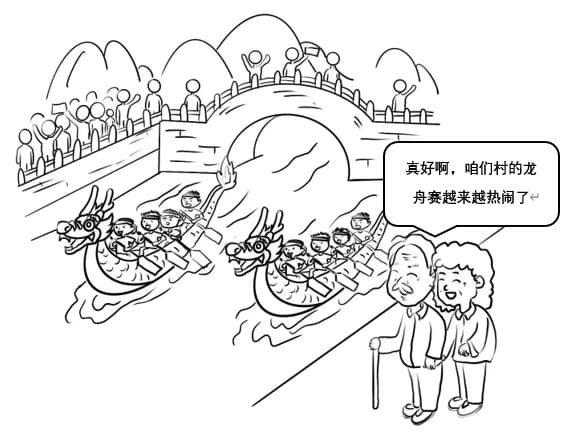
\includegraphics[width=0.55\linewidth]{picture/2023.png}
\end{figure}


%







\end{document}